\documentclass{scrartcl}

	\usepackage{jupyterlatex}

    \usepackage[breakable]{tcolorbox}
    

    % Basic figure setup, for now with no caption control since it's done
    % automatically by Pandoc (which extracts ![](path) syntax from Markdown).
    \usepackage{graphicx}
    % Maintain compatibility with old templates. Remove in nbconvert 6.0
    \let\Oldincludegraphics\includegraphics
    % Ensure that by default, figures have no caption (until we provide a
    % proper Figure object with a Caption API and a way to capture that
    % in the conversion process - todo).
    \usepackage{caption}
    \DeclareCaptionFormat{nocaption}{}
    \captionsetup{format=nocaption,aboveskip=0pt,belowskip=0pt}

    \usepackage{float}
    \floatplacement{figure}{H} % forces figures to be placed at the correct location
    \usepackage{xcolor} % Allow colors to be defined
    \usepackage{enumerate} % Needed for markdown enumerations to work
    \usepackage{geometry} % Used to adjust the document margins
    \usepackage{amsmath} % Equations
    \usepackage{amssymb} % Equations
    \usepackage{textcomp} % defines textquotesingle
    % Hack from http://tex.stackexchange.com/a/47451/13684:
    \AtBeginDocument{%
        \def\PYZsq{\textquotesingle}% Upright quotes in Pygmentized code
    }
    \usepackage{upquote} % Upright quotes for verbatim code
    \usepackage{eurosym} % defines \euro

    \usepackage{iftex}
    \ifPDFTeX
        \usepackage[T1]{fontenc}
        \IfFileExists{alphabeta.sty}{
              \usepackage{alphabeta}
          }{
              \usepackage[mathletters]{ucs}
              \usepackage[utf8]{inputenc}
          }
    \else
        \usepackage{fontspec}
        \usepackage{unicode-math}
    \fi

    \usepackage{fancyvrb} % verbatim replacement that allows latex
    \usepackage{grffile} % extends the file name processing of package graphics
                         % to support a larger range
    \makeatletter % fix for old versions of grffile with XeLaTeX
    \@ifpackagelater{grffile}{2019/11/01}
    {
      % Do nothing on new versions
    }
    {
      \def\Gread@@xetex#1{%
        \IfFileExists{"\Gin@base".bb}%
        {\Gread@eps{\Gin@base.bb}}%
        {\Gread@@xetex@aux#1}%
      }
    }
    \makeatother
    \usepackage[Export]{adjustbox} % Used to constrain images to a maximum size
    \adjustboxset{max size={0.9\linewidth}{0.9\paperheight}}

    % The hyperref package gives us a pdf with properly built
    % internal navigation ('pdf bookmarks' for the table of contents,
    % internal cross-reference links, web links for URLs, etc.)
    \usepackage{hyperref}
    % The default LaTeX title has an obnoxious amount of whitespace. By default,
    % titling removes some of it. It also provides customization options.
    \usepackage{longtable} % longtable support required by pandoc >1.10
    \usepackage{booktabs}  % table support for pandoc > 1.12.2
    \usepackage{array}     % table support for pandoc >= 2.11.3
    \usepackage{calc}      % table minipage width calculation for pandoc >= 2.11.1
    \usepackage[inline]{enumitem} % IRkernel/repr support (it uses the enumerate* environment)
    \usepackage[normalem]{ulem} % ulem is needed to support strikethroughs (\sout)
                                % normalem makes italics be italics, not underlines
    \usepackage{mathrsfs}
    

    
    % Colors for the hyperref package
    \definecolor{urlcolor}{rgb}{0,.145,.698}
    \definecolor{linkcolor}{rgb}{.71,0.21,0.01}
    \definecolor{citecolor}{rgb}{.12,.54,.11}

    % ANSI colors
    \definecolor{ansi-black}{HTML}{3E424D}
    \definecolor{ansi-black-intense}{HTML}{282C36}
    \definecolor{ansi-red}{HTML}{E75C58}
    \definecolor{ansi-red-intense}{HTML}{B22B31}
    \definecolor{ansi-green}{HTML}{00A250}
    \definecolor{ansi-green-intense}{HTML}{007427}
    \definecolor{ansi-yellow}{HTML}{DDB62B}
    \definecolor{ansi-yellow-intense}{HTML}{B27D12}
    \definecolor{ansi-blue}{HTML}{208FFB}
    \definecolor{ansi-blue-intense}{HTML}{0065CA}
    \definecolor{ansi-magenta}{HTML}{D160C4}
    \definecolor{ansi-magenta-intense}{HTML}{A03196}
    \definecolor{ansi-cyan}{HTML}{60C6C8}
    \definecolor{ansi-cyan-intense}{HTML}{258F8F}
    \definecolor{ansi-white}{HTML}{C5C1B4}
    \definecolor{ansi-white-intense}{HTML}{A1A6B2}
    \definecolor{ansi-default-inverse-fg}{HTML}{FFFFFF}
    \definecolor{ansi-default-inverse-bg}{HTML}{000000}

    % common color for the border for error outputs.
    \definecolor{outerrorbackground}{HTML}{FFDFDF}

    % commands and environments needed by pandoc snippets
    % extracted from the output of `pandoc -s`
    \providecommand{\tightlist}{%
      \setlength{\itemsep}{0pt}\setlength{\parskip}{0pt}}
    \DefineVerbatimEnvironment{Highlighting}{Verbatim}{commandchars=\\\{\}}
    % Add ',fontsize=\small' for more characters per line
    \newenvironment{Shaded}{}{}
    \newcommand{\KeywordTok}[1]{\textcolor[rgb]{0.00,0.44,0.13}{\textbf{{#1}}}}
    \newcommand{\DataTypeTok}[1]{\textcolor[rgb]{0.56,0.13,0.00}{{#1}}}
    \newcommand{\DecValTok}[1]{\textcolor[rgb]{0.25,0.63,0.44}{{#1}}}
    \newcommand{\BaseNTok}[1]{\textcolor[rgb]{0.25,0.63,0.44}{{#1}}}
    \newcommand{\FloatTok}[1]{\textcolor[rgb]{0.25,0.63,0.44}{{#1}}}
    \newcommand{\CharTok}[1]{\textcolor[rgb]{0.25,0.44,0.63}{{#1}}}
    \newcommand{\StringTok}[1]{\textcolor[rgb]{0.25,0.44,0.63}{{#1}}}
    \newcommand{\CommentTok}[1]{\textcolor[rgb]{0.38,0.63,0.69}{\textit{{#1}}}}
    \newcommand{\OtherTok}[1]{\textcolor[rgb]{0.00,0.44,0.13}{{#1}}}
    \newcommand{\AlertTok}[1]{\textcolor[rgb]{1.00,0.00,0.00}{\textbf{{#1}}}}
    \newcommand{\FunctionTok}[1]{\textcolor[rgb]{0.02,0.16,0.49}{{#1}}}
    \newcommand{\RegionMarkerTok}[1]{{#1}}
    \newcommand{\ErrorTok}[1]{\textcolor[rgb]{1.00,0.00,0.00}{\textbf{{#1}}}}
    \newcommand{\NormalTok}[1]{{#1}}

    % Additional commands for more recent versions of Pandoc
    \newcommand{\ConstantTok}[1]{\textcolor[rgb]{0.53,0.00,0.00}{{#1}}}
    \newcommand{\SpecialCharTok}[1]{\textcolor[rgb]{0.25,0.44,0.63}{{#1}}}
    \newcommand{\VerbatimStringTok}[1]{\textcolor[rgb]{0.25,0.44,0.63}{{#1}}}
    \newcommand{\SpecialStringTok}[1]{\textcolor[rgb]{0.73,0.40,0.53}{{#1}}}
    \newcommand{\ImportTok}[1]{{#1}}
    \newcommand{\DocumentationTok}[1]{\textcolor[rgb]{0.73,0.13,0.13}{\textit{{#1}}}}
    \newcommand{\AnnotationTok}[1]{\textcolor[rgb]{0.38,0.63,0.69}{\textbf{\textit{{#1}}}}}
    \newcommand{\CommentVarTok}[1]{\textcolor[rgb]{0.38,0.63,0.69}{\textbf{\textit{{#1}}}}}
    \newcommand{\VariableTok}[1]{\textcolor[rgb]{0.10,0.09,0.49}{{#1}}}
    \newcommand{\ControlFlowTok}[1]{\textcolor[rgb]{0.00,0.44,0.13}{\textbf{{#1}}}}
    \newcommand{\OperatorTok}[1]{\textcolor[rgb]{0.40,0.40,0.40}{{#1}}}
    \newcommand{\BuiltInTok}[1]{{#1}}
    \newcommand{\ExtensionTok}[1]{{#1}}
    \newcommand{\PreprocessorTok}[1]{\textcolor[rgb]{0.74,0.48,0.00}{{#1}}}
    \newcommand{\AttributeTok}[1]{\textcolor[rgb]{0.49,0.56,0.16}{{#1}}}
    \newcommand{\InformationTok}[1]{\textcolor[rgb]{0.38,0.63,0.69}{\textbf{\textit{{#1}}}}}
    \newcommand{\WarningTok}[1]{\textcolor[rgb]{0.38,0.63,0.69}{\textbf{\textit{{#1}}}}}


    % Define a nice break command that doesn't care if a line doesn't already
    % exist.
    \def\br{\hspace*{\fill} \\* }
    % Math Jax compatibility definitions
    \def\gt{>}
    \def\lt{<}
    \let\Oldtex\TeX
    \let\Oldlatex\LaTeX
    \renewcommand{\TeX}{\textrm{\Oldtex}}
    \renewcommand{\LaTeX}{\textrm{\Oldlatex}}
    % Document parameters
    % Document title
    \newcommand*{\unitcounter}{10}
    \addtocounter{section}{\unitcounter}
    \addtocounter{section}{-1}
    \newcommand*{\mytitle}{Unit \unitcounter: Introduction to supervised learning}

	% Included at the bottom of the preamble

\title{\mytitle}
\author{Richard Foltyn}
\institute{University of Glasgow}
\hypersetup{pdfauthor={Richard Foltyn}, pdftitle={\mytitle}}

% needed to access graphs in lectures/solutions folder
\graphicspath{{../lectures/}}


    
    
    
    
    
% Pygments definitions
\makeatletter
\def\PY@reset{\let\PY@it=\relax \let\PY@bf=\relax%
    \let\PY@ul=\relax \let\PY@tc=\relax%
    \let\PY@bc=\relax \let\PY@ff=\relax}
\def\PY@tok#1{\csname PY@tok@#1\endcsname}
\def\PY@toks#1+{\ifx\relax#1\empty\else%
    \PY@tok{#1}\expandafter\PY@toks\fi}
\def\PY@do#1{\PY@bc{\PY@tc{\PY@ul{%
    \PY@it{\PY@bf{\PY@ff{#1}}}}}}}
\def\PY#1#2{\PY@reset\PY@toks#1+\relax+\PY@do{#2}}

\@namedef{PY@tok@w}{\def\PY@tc##1{\textcolor[rgb]{0.73,0.73,0.73}{##1}}}
\@namedef{PY@tok@c}{\let\PY@it=\textit\def\PY@tc##1{\textcolor[rgb]{0.24,0.48,0.48}{##1}}}
\@namedef{PY@tok@cp}{\def\PY@tc##1{\textcolor[rgb]{0.61,0.40,0.00}{##1}}}
\@namedef{PY@tok@k}{\let\PY@bf=\textbf\def\PY@tc##1{\textcolor[rgb]{0.00,0.50,0.00}{##1}}}
\@namedef{PY@tok@kp}{\def\PY@tc##1{\textcolor[rgb]{0.00,0.50,0.00}{##1}}}
\@namedef{PY@tok@kt}{\def\PY@tc##1{\textcolor[rgb]{0.69,0.00,0.25}{##1}}}
\@namedef{PY@tok@o}{\def\PY@tc##1{\textcolor[rgb]{0.40,0.40,0.40}{##1}}}
\@namedef{PY@tok@ow}{\let\PY@bf=\textbf\def\PY@tc##1{\textcolor[rgb]{0.67,0.13,1.00}{##1}}}
\@namedef{PY@tok@nb}{\def\PY@tc##1{\textcolor[rgb]{0.00,0.50,0.00}{##1}}}
\@namedef{PY@tok@nf}{\def\PY@tc##1{\textcolor[rgb]{0.00,0.00,1.00}{##1}}}
\@namedef{PY@tok@nc}{\let\PY@bf=\textbf\def\PY@tc##1{\textcolor[rgb]{0.00,0.00,1.00}{##1}}}
\@namedef{PY@tok@nn}{\let\PY@bf=\textbf\def\PY@tc##1{\textcolor[rgb]{0.00,0.00,1.00}{##1}}}
\@namedef{PY@tok@ne}{\let\PY@bf=\textbf\def\PY@tc##1{\textcolor[rgb]{0.80,0.25,0.22}{##1}}}
\@namedef{PY@tok@nv}{\def\PY@tc##1{\textcolor[rgb]{0.10,0.09,0.49}{##1}}}
\@namedef{PY@tok@no}{\def\PY@tc##1{\textcolor[rgb]{0.53,0.00,0.00}{##1}}}
\@namedef{PY@tok@nl}{\def\PY@tc##1{\textcolor[rgb]{0.46,0.46,0.00}{##1}}}
\@namedef{PY@tok@ni}{\let\PY@bf=\textbf\def\PY@tc##1{\textcolor[rgb]{0.44,0.44,0.44}{##1}}}
\@namedef{PY@tok@na}{\def\PY@tc##1{\textcolor[rgb]{0.41,0.47,0.13}{##1}}}
\@namedef{PY@tok@nt}{\let\PY@bf=\textbf\def\PY@tc##1{\textcolor[rgb]{0.00,0.50,0.00}{##1}}}
\@namedef{PY@tok@nd}{\def\PY@tc##1{\textcolor[rgb]{0.67,0.13,1.00}{##1}}}
\@namedef{PY@tok@s}{\def\PY@tc##1{\textcolor[rgb]{0.73,0.13,0.13}{##1}}}
\@namedef{PY@tok@sd}{\let\PY@it=\textit\def\PY@tc##1{\textcolor[rgb]{0.73,0.13,0.13}{##1}}}
\@namedef{PY@tok@si}{\let\PY@bf=\textbf\def\PY@tc##1{\textcolor[rgb]{0.64,0.35,0.47}{##1}}}
\@namedef{PY@tok@se}{\let\PY@bf=\textbf\def\PY@tc##1{\textcolor[rgb]{0.67,0.36,0.12}{##1}}}
\@namedef{PY@tok@sr}{\def\PY@tc##1{\textcolor[rgb]{0.64,0.35,0.47}{##1}}}
\@namedef{PY@tok@ss}{\def\PY@tc##1{\textcolor[rgb]{0.10,0.09,0.49}{##1}}}
\@namedef{PY@tok@sx}{\def\PY@tc##1{\textcolor[rgb]{0.00,0.50,0.00}{##1}}}
\@namedef{PY@tok@m}{\def\PY@tc##1{\textcolor[rgb]{0.40,0.40,0.40}{##1}}}
\@namedef{PY@tok@gh}{\let\PY@bf=\textbf\def\PY@tc##1{\textcolor[rgb]{0.00,0.00,0.50}{##1}}}
\@namedef{PY@tok@gu}{\let\PY@bf=\textbf\def\PY@tc##1{\textcolor[rgb]{0.50,0.00,0.50}{##1}}}
\@namedef{PY@tok@gd}{\def\PY@tc##1{\textcolor[rgb]{0.63,0.00,0.00}{##1}}}
\@namedef{PY@tok@gi}{\def\PY@tc##1{\textcolor[rgb]{0.00,0.52,0.00}{##1}}}
\@namedef{PY@tok@gr}{\def\PY@tc##1{\textcolor[rgb]{0.89,0.00,0.00}{##1}}}
\@namedef{PY@tok@ge}{\let\PY@it=\textit}
\@namedef{PY@tok@gs}{\let\PY@bf=\textbf}
\@namedef{PY@tok@gp}{\let\PY@bf=\textbf\def\PY@tc##1{\textcolor[rgb]{0.00,0.00,0.50}{##1}}}
\@namedef{PY@tok@go}{\def\PY@tc##1{\textcolor[rgb]{0.44,0.44,0.44}{##1}}}
\@namedef{PY@tok@gt}{\def\PY@tc##1{\textcolor[rgb]{0.00,0.27,0.87}{##1}}}
\@namedef{PY@tok@err}{\def\PY@bc##1{{\setlength{\fboxsep}{\string -\fboxrule}\fcolorbox[rgb]{1.00,0.00,0.00}{1,1,1}{\strut ##1}}}}
\@namedef{PY@tok@kc}{\let\PY@bf=\textbf\def\PY@tc##1{\textcolor[rgb]{0.00,0.50,0.00}{##1}}}
\@namedef{PY@tok@kd}{\let\PY@bf=\textbf\def\PY@tc##1{\textcolor[rgb]{0.00,0.50,0.00}{##1}}}
\@namedef{PY@tok@kn}{\let\PY@bf=\textbf\def\PY@tc##1{\textcolor[rgb]{0.00,0.50,0.00}{##1}}}
\@namedef{PY@tok@kr}{\let\PY@bf=\textbf\def\PY@tc##1{\textcolor[rgb]{0.00,0.50,0.00}{##1}}}
\@namedef{PY@tok@bp}{\def\PY@tc##1{\textcolor[rgb]{0.00,0.50,0.00}{##1}}}
\@namedef{PY@tok@fm}{\def\PY@tc##1{\textcolor[rgb]{0.00,0.00,1.00}{##1}}}
\@namedef{PY@tok@vc}{\def\PY@tc##1{\textcolor[rgb]{0.10,0.09,0.49}{##1}}}
\@namedef{PY@tok@vg}{\def\PY@tc##1{\textcolor[rgb]{0.10,0.09,0.49}{##1}}}
\@namedef{PY@tok@vi}{\def\PY@tc##1{\textcolor[rgb]{0.10,0.09,0.49}{##1}}}
\@namedef{PY@tok@vm}{\def\PY@tc##1{\textcolor[rgb]{0.10,0.09,0.49}{##1}}}
\@namedef{PY@tok@sa}{\def\PY@tc##1{\textcolor[rgb]{0.73,0.13,0.13}{##1}}}
\@namedef{PY@tok@sb}{\def\PY@tc##1{\textcolor[rgb]{0.73,0.13,0.13}{##1}}}
\@namedef{PY@tok@sc}{\def\PY@tc##1{\textcolor[rgb]{0.73,0.13,0.13}{##1}}}
\@namedef{PY@tok@dl}{\def\PY@tc##1{\textcolor[rgb]{0.73,0.13,0.13}{##1}}}
\@namedef{PY@tok@s2}{\def\PY@tc##1{\textcolor[rgb]{0.73,0.13,0.13}{##1}}}
\@namedef{PY@tok@sh}{\def\PY@tc##1{\textcolor[rgb]{0.73,0.13,0.13}{##1}}}
\@namedef{PY@tok@s1}{\def\PY@tc##1{\textcolor[rgb]{0.73,0.13,0.13}{##1}}}
\@namedef{PY@tok@mb}{\def\PY@tc##1{\textcolor[rgb]{0.40,0.40,0.40}{##1}}}
\@namedef{PY@tok@mf}{\def\PY@tc##1{\textcolor[rgb]{0.40,0.40,0.40}{##1}}}
\@namedef{PY@tok@mh}{\def\PY@tc##1{\textcolor[rgb]{0.40,0.40,0.40}{##1}}}
\@namedef{PY@tok@mi}{\def\PY@tc##1{\textcolor[rgb]{0.40,0.40,0.40}{##1}}}
\@namedef{PY@tok@il}{\def\PY@tc##1{\textcolor[rgb]{0.40,0.40,0.40}{##1}}}
\@namedef{PY@tok@mo}{\def\PY@tc##1{\textcolor[rgb]{0.40,0.40,0.40}{##1}}}
\@namedef{PY@tok@ch}{\let\PY@it=\textit\def\PY@tc##1{\textcolor[rgb]{0.24,0.48,0.48}{##1}}}
\@namedef{PY@tok@cm}{\let\PY@it=\textit\def\PY@tc##1{\textcolor[rgb]{0.24,0.48,0.48}{##1}}}
\@namedef{PY@tok@cpf}{\let\PY@it=\textit\def\PY@tc##1{\textcolor[rgb]{0.24,0.48,0.48}{##1}}}
\@namedef{PY@tok@c1}{\let\PY@it=\textit\def\PY@tc##1{\textcolor[rgb]{0.24,0.48,0.48}{##1}}}
\@namedef{PY@tok@cs}{\let\PY@it=\textit\def\PY@tc##1{\textcolor[rgb]{0.24,0.48,0.48}{##1}}}

\def\PYZbs{\char`\\}
\def\PYZus{\char`\_}
\def\PYZob{\char`\{}
\def\PYZcb{\char`\}}
\def\PYZca{\char`\^}
\def\PYZam{\char`\&}
\def\PYZlt{\char`\<}
\def\PYZgt{\char`\>}
\def\PYZsh{\char`\#}
\def\PYZpc{\char`\%}
\def\PYZdl{\char`\$}
\def\PYZhy{\char`\-}
\def\PYZsq{\char`\'}
\def\PYZdq{\char`\"}
\def\PYZti{\char`\~}
% for compatibility with earlier versions
\def\PYZat{@}
\def\PYZlb{[}
\def\PYZrb{]}
\makeatother


    % For linebreaks inside Verbatim environment from package fancyvrb.
    \makeatletter
        \newbox\Wrappedcontinuationbox
        \newbox\Wrappedvisiblespacebox
        \newcommand*\Wrappedvisiblespace {\textcolor{red}{\textvisiblespace}}
        \newcommand*\Wrappedcontinuationsymbol {\textcolor{red}{\llap{\tiny$\m@th\hookrightarrow$}}}
        \newcommand*\Wrappedcontinuationindent {3ex }
        \newcommand*\Wrappedafterbreak {\kern\Wrappedcontinuationindent\copy\Wrappedcontinuationbox}
        % Take advantage of the already applied Pygments mark-up to insert
        % potential linebreaks for TeX processing.
        %        {, <, #, %, $, ' and ": go to next line.
        %        _, }, ^, &, >, - and ~: stay at end of broken line.
        % Use of \textquotesingle for straight quote.
        \newcommand*\Wrappedbreaksatspecials {%
            \def\PYGZus{\discretionary{\char`\_}{\Wrappedafterbreak}{\char`\_}}%
            \def\PYGZob{\discretionary{}{\Wrappedafterbreak\char`\{}{\char`\{}}%
            \def\PYGZcb{\discretionary{\char`\}}{\Wrappedafterbreak}{\char`\}}}%
            \def\PYGZca{\discretionary{\char`\^}{\Wrappedafterbreak}{\char`\^}}%
            \def\PYGZam{\discretionary{\char`\&}{\Wrappedafterbreak}{\char`\&}}%
            \def\PYGZlt{\discretionary{}{\Wrappedafterbreak\char`\<}{\char`\<}}%
            \def\PYGZgt{\discretionary{\char`\>}{\Wrappedafterbreak}{\char`\>}}%
            \def\PYGZsh{\discretionary{}{\Wrappedafterbreak\char`\#}{\char`\#}}%
            \def\PYGZpc{\discretionary{}{\Wrappedafterbreak\char`\%}{\char`\%}}%
            \def\PYGZdl{\discretionary{}{\Wrappedafterbreak\char`\$}{\char`\$}}%
            \def\PYGZhy{\discretionary{\char`\-}{\Wrappedafterbreak}{\char`\-}}%
            \def\PYGZsq{\discretionary{}{\Wrappedafterbreak\textquotesingle}{\textquotesingle}}%
            \def\PYGZdq{\discretionary{}{\Wrappedafterbreak\char`\"}{\char`\"}}%
            \def\PYGZti{\discretionary{\char`\~}{\Wrappedafterbreak}{\char`\~}}%
        }
        % Some characters . , ; ? ! / are not pygmentized.
        % This macro makes them "active" and they will insert potential linebreaks
        \newcommand*\Wrappedbreaksatpunct {%
            \lccode`\~`\.\lowercase{\def~}{\discretionary{\hbox{\char`\.}}{\Wrappedafterbreak}{\hbox{\char`\.}}}%
            \lccode`\~`\,\lowercase{\def~}{\discretionary{\hbox{\char`\,}}{\Wrappedafterbreak}{\hbox{\char`\,}}}%
            \lccode`\~`\;\lowercase{\def~}{\discretionary{\hbox{\char`\;}}{\Wrappedafterbreak}{\hbox{\char`\;}}}%
            \lccode`\~`\:\lowercase{\def~}{\discretionary{\hbox{\char`\:}}{\Wrappedafterbreak}{\hbox{\char`\:}}}%
            \lccode`\~`\?\lowercase{\def~}{\discretionary{\hbox{\char`\?}}{\Wrappedafterbreak}{\hbox{\char`\?}}}%
            \lccode`\~`\!\lowercase{\def~}{\discretionary{\hbox{\char`\!}}{\Wrappedafterbreak}{\hbox{\char`\!}}}%
            \lccode`\~`\/\lowercase{\def~}{\discretionary{\hbox{\char`\/}}{\Wrappedafterbreak}{\hbox{\char`\/}}}%
            \catcode`\.\active
            \catcode`\,\active
            \catcode`\;\active
            \catcode`\:\active
            \catcode`\?\active
            \catcode`\!\active
            \catcode`\/\active
            \lccode`\~`\~
        }
    \makeatother

    \let\OriginalVerbatim=\Verbatim
    \makeatletter
    \renewcommand{\Verbatim}[1][1]{%
        %\parskip\z@skip
        \sbox\Wrappedcontinuationbox {\Wrappedcontinuationsymbol}%
        \sbox\Wrappedvisiblespacebox {\FV@SetupFont\Wrappedvisiblespace}%
        \def\FancyVerbFormatLine ##1{\hsize\linewidth
            \vtop{\raggedright\hyphenpenalty\z@\exhyphenpenalty\z@
                \doublehyphendemerits\z@\finalhyphendemerits\z@
                \strut ##1\strut}%
        }%
        % If the linebreak is at a space, the latter will be displayed as visible
        % space at end of first line, and a continuation symbol starts next line.
        % Stretch/shrink are however usually zero for typewriter font.
        \def\FV@Space {%
            \nobreak\hskip\z@ plus\fontdimen3\font minus\fontdimen4\font
            \discretionary{\copy\Wrappedvisiblespacebox}{\Wrappedafterbreak}
            {\kern\fontdimen2\font}%
        }%

        % Allow breaks at special characters using \PYG... macros.
        \Wrappedbreaksatspecials
        % Breaks at punctuation characters . , ; ? ! and / need catcode=\active
        \OriginalVerbatim[#1,fontsize=\small,codes*=\Wrappedbreaksatpunct]%
    }
    \makeatother

    % Exact colors from NB
    \definecolor{incolor}{HTML}{303F9F}
    \definecolor{outcolor}{HTML}{D84315}
    \definecolor{cellborder}{HTML}{CFCFCF}
    \definecolor{cellbackground}{HTML}{FCFCFC}

    % prompt
    \makeatletter
    \newcommand{\boxspacing}{\kern\kvtcb@left@rule\kern\kvtcb@boxsep}
    \makeatother
    \newcommand{\prompt}[4]{
        {\ttfamily\llap{{\color{#2}[#3]:\hspace{3pt}#4}}\vspace{-\baselineskip}}
    }
    

    
    % Prevent overflowing lines due to hard-to-break entities
    \sloppy
    % Setup hyperref package
    \hypersetup{
      breaklinks=true,  % so long urls are correctly broken across lines
      colorlinks=true,
      urlcolor=urlcolor,
      linkcolor=linkcolor,
      citecolor=citecolor,
      }
    % Slightly bigger margins than the latex defaults
    
    \geometry{verbose,tmargin=1in,bmargin=1in,lmargin=1in,rmargin=1in}
    
    

\begin{document}
    
    \maketitle
	\tableofcontents
    
    

    
    \hypertarget{introduction-to-supervised-learning}{%
\section{Introduction to supervised
learning}\label{introduction-to-supervised-learning}}

    \hypertarget{simple-univariate-linear-regression}{%
\subsection{Simple (univariate) linear
regression}\label{simple-univariate-linear-regression}}

Imagine the simplest linear model where the dependent variable \(y\) is
assumed to be an affine function of the explanatory variable \(x\) and
an error term \(\epsilon\), given by \[
y_i = \alpha + \beta x_i + \epsilon_i
\] for each observation \(i\). In econometrics, the parameters
\(\alpha\) and \(\beta\) are called the intercept and slope parameters,
respectively. In machine learning, the terminology often differs and you
might see a simple linear model written like \[
y_i = b + w x_i + \epsilon_i
\] where \(b\) is called the \emph{bias} and \(w\) is called a
\emph{weight}.

Our goal is to estimate the parameters \(\alpha\) and \(\beta\) which is
most commonly done by ordinary least squares (OLS). OLS is defined as
the estimator that finds the estimates
\((\widehat{\alpha}, \widehat{\beta})\) such that the sum of squared
errors is minimized, \[
L(\alpha, \beta) = \frac{1}{N}
    \sum_i^N \Bigl(y_i - \alpha - \beta x_i \Bigr)^2
\] where \(L\) is the loss function that depends on the choice of
parameters. Note that we use the ``hat'' notation \(\widehat{\alpha}\)
to distinguish the OLS estimate from the (usually unknown) true
parameter \(\alpha\). The exact values of \(\widehat{\alpha}\) and
\(\widehat{\beta}\) will vary depending the sample size and estimator
used as we will see later in this unit.

For this simple model, the estimates are given by the expressions \[
\begin{aligned}
\widehat{\beta} &= \frac{\widehat{Cov}(y,x)}{\widehat{Var}(x)} \\
\widehat{\alpha} &= \overline{y} - \widehat{\beta} \overline{x}
\end{aligned}
\] where \(\widehat{Cov}(\bullet,\bullet)\) and
\(\widehat{Var}(\bullet)\) are the \emph{sample} covariance and
variance, respectively, and \(\overline{y}\) and \(\overline{x}\) are
the sample means of \(y\) and \(x\).

There is a straightforward generalization to the multivariate setting
where we have a vector \(\mathbf{x}_i\) of explanatory variables (which
usually include the intercept) and a parameter vector \(\bm\beta\)
so that the model is given by \[
y_i = \mathbf{x}_i'\bm\beta + \epsilon_i
\] If we stack all \(\mathbf{x}_i\) in the matrix \(\mathbf{X}\) and all
\(y_i\) in the vector \(\mathbf{y}\), the OLS estimate of
\(\bm\beta\) is given by the well-known formula \[
\widehat{\bm\beta} = \left(\mathbf{X}'\mathbf{X}\right)^{-1} \mathbf{X}'\mathbf{y}
\]

However, we will not be estimating linear regressions based on this
formula and you should never attempt this, as naively implementing such
matrix operations can lead to numerical problems. Instead, always use
pre-packaged least-squares solvers such as those implemented in NumPy's
\href{https://numpy.org/doc/stable/reference/generated/numpy.linalg.lstsq.html}{\texttt{lstsq()}}
or SciPy's
\href{https://docs.scipy.org/doc/scipy/reference/generated/scipy.linalg.lstsq.html}{\texttt{lstsq()}}
functions. For econometrics and machine learning, it usually makes sense
to use linear regression models such as those implemented in
\href{https://www.statsmodels.org/stable/regression.html}{\texttt{statsmodels}}
or
\href{https://scikit-learn.org/stable/modules/generated/sklearn.linear_model.LinearRegression.html}{\texttt{scikit-learn}},
which is what we turn to next.

    \hypertarget{univariate-linear-regressions-with-scikit-learn}{%
\subsubsection{Univariate linear regressions with
scikit-learn}\label{univariate-linear-regressions-with-scikit-learn}}

We start by fitting the simple linear model \[
y_i = \alpha + \beta x_i + \epsilon_i
\] using \texttt{scikit-learn}. For now, we proceed using synthetically
generated data where we know the true relationship, assuming that \[
\begin{aligned}
y_i &= 1 + \frac{1}{2} x_i + \epsilon_i \\
\epsilon &\stackrel{\text{iid}}{\sim} N(0, 0.7^2)
\end{aligned}
\] so that the true parameters are \(\alpha = 1\) and
\(\beta = \frac{1}{2}\). The error term \(\epsilon\) is assumed to be
normally distributed with mean \(0\) and variance \(0.7^2 = 0.49\). Note
that it is customary to specify the normal distribution in terms of its
variance (here \(0.49\)), but most NumPy and SciPy functions expect the
standard deviation (here \(0.7\)) to be passed as the scale parameter of
a normal distribution.

We generate a sample of \(N=30\) observations as follows:

    \begin{tcolorbox}[breakable, size=fbox, boxrule=1pt, pad at break*=1mm,colback=cellbackground, colframe=cellborder]
\prompt{In}{incolor}{1}{\boxspacing}
\begin{Verbatim}[commandchars=\\\{\}]
\PY{k+kn}{import} \PY{n+nn}{numpy} \PY{k}{as} \PY{n+nn}{np}
\PY{k+kn}{from} \PY{n+nn}{numpy}\PY{n+nn}{.}\PY{n+nn}{random} \PY{k+kn}{import} \PY{n}{default\PYZus{}rng}

\PY{n}{rng} \PY{o}{=} \PY{n}{default\PYZus{}rng}\PY{p}{(}\PY{l+m+mi}{123}\PY{p}{)}

\PY{c+c1}{\PYZsh{} Number of observations}
\PY{n}{N} \PY{o}{=} \PY{l+m+mi}{30}

\PY{c+c1}{\PYZsh{} True parameters}
\PY{n}{alpha} \PY{o}{=} \PY{l+m+mf}{1.0}
\PY{n}{beta} \PY{o}{=} \PY{l+m+mf}{0.5}

\PY{c+c1}{\PYZsh{} Use x that are uniformly spaced on [0, 10]}
\PY{n}{x} \PY{o}{=} \PY{n}{np}\PY{o}{.}\PY{n}{linspace}\PY{p}{(}\PY{l+m+mi}{0}\PY{p}{,} \PY{l+m+mi}{10}\PY{p}{,} \PY{n}{N}\PY{p}{)}
\PY{c+c1}{\PYZsh{} Normally distributed errors}
\PY{n}{epsilon} \PY{o}{=} \PY{n}{rng}\PY{o}{.}\PY{n}{normal}\PY{p}{(}\PY{n}{scale}\PY{o}{=}\PY{l+m+mf}{0.7}\PY{p}{,} \PY{n}{size}\PY{o}{=}\PY{n}{N}\PY{p}{)}
\PY{c+c1}{\PYZsh{} Create outcome variable}
\PY{n}{y} \PY{o}{=} \PY{n}{alpha} \PY{o}{+} \PY{n}{beta} \PY{o}{*} \PY{n}{x} \PY{o}{+} \PY{n}{epsilon}
\end{Verbatim}
\end{tcolorbox}

    To fit a linear model, we use the
\href{https://scikit-learn.org/stable/modules/generated/sklearn.linear_model.LinearRegression.html}{\texttt{LinearRegression}}
class provided by \texttt{scikit-learn}. Before doing so, we need to
import it from \texttt{sklearn.linear\_model}. Note that most fitting
routines in \texttt{scikit-learn} expect a \emph{matrix} as opposed to a
vector even if the model has only one explanatory variable, so we need
to insert an artificial axis to create the matrix
\texttt{X\ =\ x{[}:,\ None{]}}.

    \begin{tcolorbox}[breakable, size=fbox, boxrule=1pt, pad at break*=1mm,colback=cellbackground, colframe=cellborder]
\prompt{In}{incolor}{2}{\boxspacing}
\begin{Verbatim}[commandchars=\\\{\}]
\PY{k+kn}{from} \PY{n+nn}{sklearn}\PY{n+nn}{.}\PY{n+nn}{linear\PYZus{}model} \PY{k+kn}{import} \PY{n}{LinearRegression}

\PY{c+c1}{\PYZsh{} Create LinearRegression object}
\PY{n}{lr} \PY{o}{=} \PY{n}{LinearRegression}\PY{p}{(}\PY{n}{fit\PYZus{}intercept}\PY{o}{=}\PY{k+kc}{True}\PY{p}{)}

\PY{c+c1}{\PYZsh{} fit() expects two\PYZhy{}dimensional object, convert to N x 1 matrix}
\PY{n}{X} \PY{o}{=} \PY{n}{x}\PY{p}{[}\PY{p}{:}\PY{p}{,} \PY{k+kc}{None}\PY{p}{]}

\PY{c+c1}{\PYZsh{} Fit model to data}
\PY{n}{lr}\PY{o}{.}\PY{n}{fit}\PY{p}{(}\PY{n}{X}\PY{p}{,} \PY{n}{y}\PY{p}{)}

\PY{c+c1}{\PYZsh{} Predict fitted values}
\PY{n}{yhat} \PY{o}{=} \PY{n}{lr}\PY{o}{.}\PY{n}{predict}\PY{p}{(}\PY{n}{X}\PY{p}{)}
\end{Verbatim}
\end{tcolorbox}

    The following code visualises the sample as a scatter plot of
\((x_i, y_i)\) and adds the fitted line (in solid orange). Intuitively,
for \(x=0\) the fitted line has the value \(\widehat{\alpha}\) (the
intercept) and its slope is equal to \(\widehat{\beta}\). Note that
\texttt{scikit-learn} models usually store the fitted model parameters
in the \texttt{coef\_} attribute (which is an array even if there is
only a single explanatory variable). If the model includes an intercept,
its fitted value is stored in the attribute \texttt{intercept\_}.

    \begin{tcolorbox}[breakable, size=fbox, boxrule=1pt, pad at break*=1mm,colback=cellbackground, colframe=cellborder]
\prompt{In}{incolor}{3}{\boxspacing}
\begin{Verbatim}[commandchars=\\\{\}]
\PY{k+kn}{import} \PY{n+nn}{matplotlib}\PY{n+nn}{.}\PY{n+nn}{pyplot} \PY{k}{as} \PY{n+nn}{plt}

\PY{c+c1}{\PYZsh{} Extract parameter estimates from LinearRegression object}
\PY{n}{alpha\PYZus{}hat} \PY{o}{=} \PY{n}{lr}\PY{o}{.}\PY{n}{intercept\PYZus{}}
\PY{n}{beta\PYZus{}hat} \PY{o}{=} \PY{n}{lr}\PY{o}{.}\PY{n}{coef\PYZus{}}\PY{p}{[}\PY{l+m+mi}{0}\PY{p}{]}

\PY{n}{fig}\PY{p}{,} \PY{n}{ax} \PY{o}{=} \PY{n}{plt}\PY{o}{.}\PY{n}{subplots}\PY{p}{(}\PY{l+m+mi}{1}\PY{p}{,} \PY{l+m+mi}{1}\PY{p}{,} \PY{n}{figsize}\PY{o}{=}\PY{p}{(}\PY{l+m+mi}{5}\PY{p}{,} \PY{l+m+mf}{3.5}\PY{p}{)}\PY{p}{)}

\PY{c+c1}{\PYZsh{} Plot true relationship}
\PY{n}{ax}\PY{o}{.}\PY{n}{axline}\PY{p}{(}\PY{p}{(}\PY{l+m+mf}{0.0}\PY{p}{,} \PY{n}{alpha}\PY{p}{)}\PY{p}{,} \PY{n}{slope}\PY{o}{=}\PY{n}{beta}\PY{p}{,} \PY{n}{lw}\PY{o}{=}\PY{l+m+mf}{1.0}\PY{p}{,} \PY{n}{ls}\PY{o}{=}\PY{l+s+s1}{\PYZsq{}}\PY{l+s+s1}{\PYZhy{}\PYZhy{}}\PY{l+s+s1}{\PYZsq{}}\PY{p}{,} \PY{n}{c}\PY{o}{=}\PY{l+s+s1}{\PYZsq{}}\PY{l+s+s1}{black}\PY{l+s+s1}{\PYZsq{}}\PY{p}{,} 
    \PY{n}{label}\PY{o}{=}\PY{l+s+sa}{r}\PY{l+s+s1}{\PYZsq{}}\PY{l+s+s1}{\PYZdl{}y = }\PY{l+s+s1}{\PYZbs{}}\PY{l+s+s1}{alpha + }\PY{l+s+s1}{\PYZbs{}}\PY{l+s+s1}{beta x\PYZdl{}}\PY{l+s+s1}{\PYZsq{}}\PY{p}{)}

\PY{c+c1}{\PYZsh{} Plot regression line}
\PY{n}{ax}\PY{o}{.}\PY{n}{axline}\PY{p}{(}\PY{p}{(}\PY{l+m+mf}{0.0}\PY{p}{,} \PY{n}{alpha\PYZus{}hat}\PY{p}{)}\PY{p}{,} \PY{n}{slope}\PY{o}{=}\PY{n}{beta\PYZus{}hat}\PY{p}{,} \PY{n}{lw}\PY{o}{=}\PY{l+m+mf}{1.0}\PY{p}{,} \PY{n}{c}\PY{o}{=}\PY{l+s+s1}{\PYZsq{}}\PY{l+s+s1}{darkorange}\PY{l+s+s1}{\PYZsq{}}\PY{p}{,} 
    \PY{n}{label}\PY{o}{=}\PY{l+s+sa}{r}\PY{l+s+s1}{\PYZsq{}}\PY{l+s+s1}{\PYZdl{}}\PY{l+s+s1}{\PYZbs{}}\PY{l+s+s1}{widehat}\PY{l+s+si}{\PYZob{}y\PYZcb{}}\PY{l+s+s1}{ = }\PY{l+s+s1}{\PYZbs{}}\PY{l+s+s1}{widehat}\PY{l+s+s1}{\PYZob{}}\PY{l+s+s1}{\PYZbs{}}\PY{l+s+s1}{alpha\PYZcb{} + }\PY{l+s+s1}{\PYZbs{}}\PY{l+s+s1}{widehat}\PY{l+s+s1}{\PYZob{}}\PY{l+s+s1}{\PYZbs{}}\PY{l+s+s1}{beta\PYZcb{} x\PYZdl{}}\PY{l+s+s1}{\PYZsq{}}\PY{p}{)}

\PY{c+c1}{\PYZsh{} Plot raw data}
\PY{n}{ax}\PY{o}{.}\PY{n}{scatter}\PY{p}{(}\PY{n}{x}\PY{p}{,} \PY{n}{y}\PY{p}{,} \PY{n}{s}\PY{o}{=}\PY{l+m+mi}{20}\PY{p}{,} \PY{n}{color}\PY{o}{=}\PY{l+s+s1}{\PYZsq{}}\PY{l+s+s1}{none}\PY{l+s+s1}{\PYZsq{}}\PY{p}{,} \PY{n}{edgecolor}\PY{o}{=}\PY{l+s+s1}{\PYZsq{}}\PY{l+s+s1}{steelblue}\PY{l+s+s1}{\PYZsq{}}\PY{p}{,} \PY{n}{alpha}\PY{o}{=}\PY{l+m+mf}{1.0}\PY{p}{,} 
    \PY{n}{lw}\PY{o}{=}\PY{l+m+mf}{0.75}\PY{p}{,} \PY{n}{label}\PY{o}{=}\PY{l+s+s1}{\PYZsq{}}\PY{l+s+s1}{y}\PY{l+s+s1}{\PYZsq{}}\PY{p}{)}

\PY{c+c1}{\PYZsh{} Plot lines connecting true and predicted values for }
\PY{c+c1}{\PYZsh{} each observation}
\PY{k}{for} \PY{n}{i} \PY{o+ow}{in} \PY{n+nb}{range}\PY{p}{(}\PY{n+nb}{len}\PY{p}{(}\PY{n}{x}\PY{p}{)}\PY{p}{)}\PY{p}{:}
    \PY{c+c1}{\PYZsh{} Predict yhat for given x\PYZus{}i}
    \PY{n}{yhat\PYZus{}i} \PY{o}{=} \PY{n}{alpha\PYZus{}hat} \PY{o}{+} \PY{n}{beta\PYZus{}hat} \PY{o}{*} \PY{n}{x}\PY{p}{[}\PY{n}{i}\PY{p}{]}
    \PY{n}{ax}\PY{o}{.}\PY{n}{plot}\PY{p}{(}\PY{p}{[}\PY{n}{x}\PY{p}{[}\PY{n}{i}\PY{p}{]}\PY{p}{,} \PY{n}{x}\PY{p}{[}\PY{n}{i}\PY{p}{]}\PY{p}{]}\PY{p}{,} \PY{p}{[}\PY{n}{y}\PY{p}{[}\PY{n}{i}\PY{p}{]}\PY{p}{,} \PY{n}{yhat\PYZus{}i}\PY{p}{]}\PY{p}{,} \PY{n}{lw}\PY{o}{=}\PY{l+m+mf}{0.5}\PY{p}{,} \PY{n}{ls}\PY{o}{=}\PY{l+s+s1}{\PYZsq{}}\PY{l+s+s1}{:}\PY{l+s+s1}{\PYZsq{}}\PY{p}{,} 
        \PY{n}{c}\PY{o}{=}\PY{l+s+s1}{\PYZsq{}}\PY{l+s+s1}{black}\PY{l+s+s1}{\PYZsq{}}\PY{p}{,} \PY{n}{alpha}\PY{o}{=}\PY{l+m+mf}{0.9}\PY{p}{)}

\PY{c+c1}{\PYZsh{} Add annotations}
\PY{n}{ax}\PY{o}{.}\PY{n}{set\PYZus{}xlabel}\PY{p}{(}\PY{l+s+s1}{\PYZsq{}}\PY{l+s+s1}{Explanatory variable: x}\PY{l+s+s1}{\PYZsq{}}\PY{p}{)}
\PY{n}{ax}\PY{o}{.}\PY{n}{set\PYZus{}ylabel}\PY{p}{(}\PY{l+s+sa}{r}\PY{l+s+s1}{\PYZsq{}}\PY{l+s+s1}{Response variable: y, \PYZdl{}}\PY{l+s+s1}{\PYZbs{}}\PY{l+s+s1}{widehat}\PY{l+s+si}{\PYZob{}y\PYZcb{}}\PY{l+s+s1}{\PYZdl{}}\PY{l+s+s1}{\PYZsq{}}\PY{p}{)}
\PY{n}{ax}\PY{o}{.}\PY{n}{axhline}\PY{p}{(}\PY{n}{alpha\PYZus{}hat}\PY{p}{,} \PY{n}{lw}\PY{o}{=}\PY{l+m+mf}{0.5}\PY{p}{,} \PY{n}{c}\PY{o}{=}\PY{l+s+s1}{\PYZsq{}}\PY{l+s+s1}{black}\PY{l+s+s1}{\PYZsq{}}\PY{p}{)}
\PY{n}{ax}\PY{o}{.}\PY{n}{legend}\PY{p}{(}\PY{n}{loc}\PY{o}{=}\PY{l+s+s1}{\PYZsq{}}\PY{l+s+s1}{best}\PY{l+s+s1}{\PYZsq{}}\PY{p}{)}
\PY{n}{ax}\PY{o}{.}\PY{n}{set\PYZus{}yticks}\PY{p}{(}\PY{p}{(}\PY{n}{alpha\PYZus{}hat}\PY{p}{,} \PY{p}{)}\PY{p}{,} \PY{p}{(}\PY{l+s+sa}{r}\PY{l+s+s1}{\PYZsq{}}\PY{l+s+s1}{\PYZdl{}}\PY{l+s+s1}{\PYZbs{}}\PY{l+s+s1}{widehat}\PY{l+s+s1}{\PYZob{}}\PY{l+s+s1}{\PYZbs{}}\PY{l+s+s1}{alpha\PYZcb{}\PYZdl{}}\PY{l+s+s1}{\PYZsq{}}\PY{p}{,} \PY{p}{)}\PY{p}{)}

\PY{n}{fig}\PY{o}{.}\PY{n}{suptitle}\PY{p}{(}\PY{l+s+s1}{\PYZsq{}}\PY{l+s+s1}{Univariate linear regression}\PY{l+s+s1}{\PYZsq{}}\PY{p}{)}
\end{Verbatim}
\end{tcolorbox}

            \begin{tcolorbox}[breakable, size=fbox, boxrule=.5pt, pad at break*=1mm, opacityfill=0]
\prompt{Out}{outcolor}{3}{\boxspacing}
\begin{Verbatim}[commandchars=\\\{\}]
Text(0.5, 0.98, 'Univariate linear regression')
\end{Verbatim}
\end{tcolorbox}
        
    \begin{center}
    \adjustimage{max size={0.9\linewidth}{0.9\paperheight}}{unit10_files/unit10_7_1.pdf}
    \end{center}
    
    The dashed black line shows the true relationship which is known in this
synthetic sample, but in general is unknown for real data. For small
sample sizes, the true and estimated parameters need not be close as the
graph illustrates. The graph also shows the prediction errors as the
dotted lines between the sample points \(y_i\) and the black fitted
model. OLS minimizes the sum of the squares of these distances.

    \hypertarget{training-and-test-samples}{%
\subsubsection{Training and test
samples}\label{training-and-test-samples}}

In econometrics, we usually emphasise \emph{inference}, \ie we are
interested in testing a hypothesis about the estimated parameter, for
example whether it is statistically different from zero. Conversely, in
machine learning the emphasis is often on prediction, \ie our goal is
to estimate a relationship from a \emph{training} sample and make
predictions for new data. Usually, we use a \emph{test} sample that is
different from the training data to assess how well our model is able to
predict outcomes for new data which has not been used for estimation.

    To demonstrate the use of training and test data sets, we use as
simplified variant of the \href{https://www.openml.org/d/42165}{Ames
house price data set} which can be obtained from
\href{https://www.openml.org}{openml.org}, a repository for free-to-use
data suitable for machine learning tasks.

The original data set has 80 features (explanatory variables) which are
characteristics of houses in Ames, a city of about 60 thousand
inhabitants in the middle of Iowa, USA. The goal is to use these
features to predict the house price (or ``target'' in ML terminology).
The above website provides details on all 80 features, but we restrict
ourselves to a small subset.

We could download the data set directly from
\href{https://www.openml.org}{openml.org} using \texttt{scikit-learn} as
follows:

\begin{Shaded}
\begin{Highlighting}[]
    \ImportTok{from}\NormalTok{ sklearn.datasets }\ImportTok{import}\NormalTok{ fetch\_openml}
\NormalTok{    ds }\OperatorTok{=}\NormalTok{ fetch\_openml(name}\OperatorTok{=}\StringTok{\textquotesingle{}house\_prices\textquotesingle{}}\NormalTok{)}

\NormalTok{    X }\OperatorTok{=}\NormalTok{ ds.data         }\CommentTok{\# Get features (explanatory variables)}
\NormalTok{    y }\OperatorTok{=}\NormalTok{ ds.target       }\CommentTok{\# get dependent variable}
\end{Highlighting}
\end{Shaded}

which returns an object with various information about the data set. The
features are stored in the \texttt{data} attribute, while the dependent
variable is stored in the \texttt{target} attribute.

Instead, we will use a local copy of the simplified data set which
contains only a subset of 12 features that are slightly adapted for our
purposes.

    \begin{tcolorbox}[breakable, size=fbox, boxrule=1pt, pad at break*=1mm,colback=cellbackground, colframe=cellborder]
\prompt{In}{incolor}{4}{\boxspacing}
\begin{Verbatim}[commandchars=\\\{\}]
\PY{c+c1}{\PYZsh{} Uncomment this to use files in the local data/ directory}
\PY{n}{DATA\PYZus{}PATH} \PY{o}{=} \PY{l+s+s1}{\PYZsq{}}\PY{l+s+s1}{../data}\PY{l+s+s1}{\PYZsq{}}

\PY{c+c1}{\PYZsh{} Load data directly from GitHub (for Google Colab)}
\PY{c+c1}{\PYZsh{} DATA\PYZus{}PATH = \PYZsq{}https://raw.githubusercontent.com/richardfoltyn/python\PYZhy{}intro\PYZhy{}PGR/main/data\PYZsq{}}
\end{Verbatim}
\end{tcolorbox}

    \begin{tcolorbox}[breakable, size=fbox, boxrule=1pt, pad at break*=1mm,colback=cellbackground, colframe=cellborder]
\prompt{In}{incolor}{5}{\boxspacing}
\begin{Verbatim}[commandchars=\\\{\}]
\PY{k+kn}{import} \PY{n+nn}{pandas} \PY{k}{as} \PY{n+nn}{pd}

\PY{n}{file} \PY{o}{=} \PY{l+s+sa}{f}\PY{l+s+s1}{\PYZsq{}}\PY{l+s+si}{\PYZob{}}\PY{n}{DATA\PYZus{}PATH}\PY{l+s+si}{\PYZcb{}}\PY{l+s+s1}{/ames\PYZus{}houses.csv}\PY{l+s+s1}{\PYZsq{}}
\PY{n}{df} \PY{o}{=} \PY{n}{pd}\PY{o}{.}\PY{n}{read\PYZus{}csv}\PY{p}{(}\PY{n}{file}\PY{p}{)}

\PY{c+c1}{\PYZsh{} List columns present in DataFrame}
\PY{n}{df}\PY{o}{.}\PY{n}{info}\PY{p}{(}\PY{p}{)}
\end{Verbatim}
\end{tcolorbox}

    \begin{Verbatim}[commandchars=\\\{\}]
<class 'pandas.core.frame.DataFrame'>
RangeIndex: 1460 entries, 0 to 1459
Data columns (total 13 columns):
 \#   Column            Non-Null Count  Dtype
---  ------            --------------  -----
 0   SalePrice         1460 non-null   float64
 1   LotArea           1460 non-null   float64
 2   Neighborhood      1460 non-null   object
 3   BuildingType      1386 non-null   object
 4   OverallQuality    1460 non-null   int64
 5   OverallCondition  1460 non-null   int64
 6   YearBuilt         1460 non-null   int64
 7   CentralAir        1460 non-null   object
 8   LivingArea        1460 non-null   float64
 9   Bathrooms         1460 non-null   int64
 10  Bedrooms          1460 non-null   int64
 11  Fireplaces        1460 non-null   int64
 12  HasGarage         1460 non-null   int64
dtypes: float64(3), int64(7), object(3)
memory usage: 148.4+ KB
    \end{Verbatim}

    In this section, we focus on the columns \texttt{SalePrice} which
contains the house price in US dollars and \texttt{LivingArea} which
contains the living area in \(m^2\) for each house in the sample. To get
some intuition for the data, we look at some descriptive statistics:

    \begin{tcolorbox}[breakable, size=fbox, boxrule=1pt, pad at break*=1mm,colback=cellbackground, colframe=cellborder]
\prompt{In}{incolor}{6}{\boxspacing}
\begin{Verbatim}[commandchars=\\\{\}]
\PY{n}{df}\PY{p}{[}\PY{p}{[}\PY{l+s+s1}{\PYZsq{}}\PY{l+s+s1}{SalePrice}\PY{l+s+s1}{\PYZsq{}}\PY{p}{,} \PY{l+s+s1}{\PYZsq{}}\PY{l+s+s1}{LivingArea}\PY{l+s+s1}{\PYZsq{}}\PY{p}{]}\PY{p}{]}\PY{o}{.}\PY{n}{describe}\PY{p}{(}\PY{p}{)}
\end{Verbatim}
\end{tcolorbox}

            \begin{tcolorbox}[breakable, size=fbox, boxrule=.5pt, pad at break*=1mm, opacityfill=0]
\prompt{Out}{outcolor}{6}{\boxspacing}
\begin{Verbatim}[commandchars=\\\{\}]
           SalePrice   LivingArea
count    1460.000000  1460.000000
mean   180921.195890   140.777444
std     79442.502883    48.813961
min     34900.000000    31.026587
25\%    129975.000000   104.923743
50\%    163000.000000   135.996777
75\%    214000.000000   165.049367
max    755000.000000   524.107798
\end{Verbatim}
\end{tcolorbox}
        
    For our analysis, we convert the \texttt{DataFrame} columns to NumPy
arrays because \texttt{scikit-learn} was not programmed to work with
pandas \texttt{DataFrames}:

    \begin{tcolorbox}[breakable, size=fbox, boxrule=1pt, pad at break*=1mm,colback=cellbackground, colframe=cellborder]
\prompt{In}{incolor}{7}{\boxspacing}
\begin{Verbatim}[commandchars=\\\{\}]
\PY{n}{features} \PY{o}{=} \PY{p}{[}\PY{l+s+s1}{\PYZsq{}}\PY{l+s+s1}{LivingArea}\PY{l+s+s1}{\PYZsq{}}\PY{p}{]}
\PY{n}{target} \PY{o}{=} \PY{l+s+s1}{\PYZsq{}}\PY{l+s+s1}{SalePrice}\PY{l+s+s1}{\PYZsq{}}

\PY{c+c1}{\PYZsh{} Convert DataFrame to NumPy arrays}
\PY{n}{y} \PY{o}{=} \PY{n}{df}\PY{p}{[}\PY{n}{target}\PY{p}{]}\PY{o}{.}\PY{n}{to\PYZus{}numpy}\PY{p}{(}\PY{p}{)}
\PY{n}{X} \PY{o}{=} \PY{n}{df}\PY{p}{[}\PY{n}{features}\PY{p}{]}\PY{o}{.}\PY{n}{to\PYZus{}numpy}\PY{p}{(}\PY{p}{)}
\end{Verbatim}
\end{tcolorbox}

    \hypertarget{manually-creating-training-and-test-samples}{%
\subsubsection*{Manually creating training and test
samples}\label{manually-creating-training-and-test-samples}}

We next want to split the data set intro training and test sub-samples.
We do this by randomly selecting a desired fraction of the data to be
part of the training sample and assign the rest to the test sample. For
this example, we assign 10\% of observations to the test sample and the
remainder to the training data set. Once we have randomly allocated 90\%
of observations to the training data set, we use the function
\href{https://numpy.org/doc/stable/reference/generated/numpy.setdiff1d.html}{\texttt{setdiff1()}}
to find the complementary test sample. This function returns the set
difference of two one-dimensional arrays, \ie all array elements from
the first argument that are \emph{not} present in the second array.

    \begin{tcolorbox}[breakable, size=fbox, boxrule=1pt, pad at break*=1mm,colback=cellbackground, colframe=cellborder]
\prompt{In}{incolor}{8}{\boxspacing}
\begin{Verbatim}[commandchars=\\\{\}]
\PY{k+kn}{import} \PY{n+nn}{numpy} \PY{k}{as} \PY{n+nn}{np}
\PY{k+kn}{from} \PY{n+nn}{numpy}\PY{n+nn}{.}\PY{n+nn}{random} \PY{k+kn}{import} \PY{n}{default\PYZus{}rng}

\PY{n}{rng} \PY{o}{=} \PY{n}{default\PYZus{}rng}\PY{p}{(}\PY{l+m+mi}{123}\PY{p}{)}

\PY{c+c1}{\PYZsh{} sample size}
\PY{n}{N} \PY{o}{=} \PY{n+nb}{len}\PY{p}{(}\PY{n}{y}\PY{p}{)}

\PY{c+c1}{\PYZsh{} fraction of data used for test sample}
\PY{n}{test\PYZus{}size} \PY{o}{=} \PY{l+m+mf}{0.1}

\PY{c+c1}{\PYZsh{} training and test sample sizes}
\PY{n}{N\PYZus{}test} \PY{o}{=} \PY{n+nb}{int}\PY{p}{(}\PY{n}{N} \PY{o}{*} \PY{n}{test\PYZus{}size}\PY{p}{)}
\PY{n}{N\PYZus{}train} \PY{o}{=} \PY{n}{N} \PY{o}{\PYZhy{}} \PY{n}{N\PYZus{}test}

\PY{c+c1}{\PYZsh{} Randomly assign observations to training samples}
\PY{n}{itrain} \PY{o}{=} \PY{n}{rng}\PY{o}{.}\PY{n}{choice}\PY{p}{(}\PY{n}{np}\PY{o}{.}\PY{n}{arange}\PY{p}{(}\PY{n}{N}\PY{p}{)}\PY{p}{,} \PY{n}{size}\PY{o}{=}\PY{n}{N\PYZus{}train}\PY{p}{,} \PY{n}{replace}\PY{o}{=}\PY{k+kc}{False}\PY{p}{)}
\PY{c+c1}{\PYZsh{} Test sample is complement of training sample}
\PY{n}{itest} \PY{o}{=} \PY{n}{np}\PY{o}{.}\PY{n}{setdiff1d}\PY{p}{(}\PY{n}{np}\PY{o}{.}\PY{n}{arange}\PY{p}{(}\PY{n}{N}\PY{p}{)}\PY{p}{,} \PY{n}{itrain}\PY{p}{)}

\PY{c+c1}{\PYZsh{} Select training sample}
\PY{n}{X\PYZus{}train} \PY{o}{=} \PY{n}{X}\PY{p}{[}\PY{n}{itrain}\PY{p}{]}
\PY{n}{y\PYZus{}train} \PY{o}{=} \PY{n}{y}\PY{p}{[}\PY{n}{itrain}\PY{p}{]}

\PY{c+c1}{\PYZsh{} Select test sample}
\PY{n}{X\PYZus{}test} \PY{o}{=} \PY{n}{X}\PY{p}{[}\PY{n}{itest}\PY{p}{]}
\PY{n}{y\PYZus{}test} \PY{o}{=} \PY{n}{y}\PY{p}{[}\PY{n}{itest}\PY{p}{]}
\end{Verbatim}
\end{tcolorbox}

    Once we have split the sample, we estimate the model on the training
sample.

    \begin{tcolorbox}[breakable, size=fbox, boxrule=1pt, pad at break*=1mm,colback=cellbackground, colframe=cellborder]
\prompt{In}{incolor}{9}{\boxspacing}
\begin{Verbatim}[commandchars=\\\{\}]
\PY{k+kn}{from} \PY{n+nn}{sklearn}\PY{n+nn}{.}\PY{n+nn}{linear\PYZus{}model} \PY{k+kn}{import} \PY{n}{LinearRegression}

\PY{c+c1}{\PYZsh{} Fit model on training sample}
\PY{n}{lr} \PY{o}{=} \PY{n}{LinearRegression}\PY{p}{(}\PY{p}{)}
\PY{n}{lr}\PY{o}{.}\PY{n}{fit}\PY{p}{(}\PY{n}{X\PYZus{}train}\PY{p}{,} \PY{n}{y\PYZus{}train}\PY{p}{)}

\PY{n+nb}{print}\PY{p}{(}\PY{l+s+s1}{\PYZsq{}}\PY{l+s+s1}{Regression coefficients}\PY{l+s+s1}{\PYZsq{}}\PY{p}{)}
\PY{n+nb}{print}\PY{p}{(}\PY{l+s+sa}{f}\PY{l+s+s1}{\PYZsq{}}\PY{l+s+s1}{  Intercept: }\PY{l+s+si}{\PYZob{}}\PY{n}{lr}\PY{o}{.}\PY{n}{intercept\PYZus{}}\PY{l+s+si}{:}\PY{l+s+s1}{.1f}\PY{l+s+si}{\PYZcb{}}\PY{l+s+s1}{\PYZsq{}}\PY{p}{)}
\PY{n+nb}{print}\PY{p}{(}\PY{l+s+sa}{f}\PY{l+s+s1}{\PYZsq{}}\PY{l+s+s1}{  Slope: }\PY{l+s+si}{\PYZob{}}\PY{n}{lr}\PY{o}{.}\PY{n}{coef\PYZus{}}\PY{p}{[}\PY{l+m+mi}{0}\PY{p}{]}\PY{l+s+si}{:}\PY{l+s+s1}{.1f}\PY{l+s+si}{\PYZcb{}}\PY{l+s+s1}{\PYZsq{}}\PY{p}{)}
\end{Verbatim}
\end{tcolorbox}

    \begin{Verbatim}[commandchars=\\\{\}]
Regression coefficients
  Intercept: 20675.0
  Slope: 1133.9
    \end{Verbatim}

    The fitted coefficients show that for each additional square meter of
living area, the sale price on average increases by \$1,134.

The following code creates a scatter plot showing the training and test
samples and adds the fitted line.

    \begin{tcolorbox}[breakable, size=fbox, boxrule=1pt, pad at break*=1mm,colback=cellbackground, colframe=cellborder]
\prompt{In}{incolor}{10}{\boxspacing}
\begin{Verbatim}[commandchars=\\\{\}]
\PY{n}{intercept} \PY{o}{=} \PY{n}{lr}\PY{o}{.}\PY{n}{intercept\PYZus{}}
\PY{n}{slope} \PY{o}{=} \PY{n}{lr}\PY{o}{.}\PY{n}{coef\PYZus{}}\PY{p}{[}\PY{l+m+mi}{0}\PY{p}{]}

\PY{n}{fig}\PY{p}{,} \PY{n}{ax} \PY{o}{=} \PY{n}{plt}\PY{o}{.}\PY{n}{subplots}\PY{p}{(}\PY{l+m+mi}{1}\PY{p}{,} \PY{l+m+mi}{1}\PY{p}{,} \PY{n}{figsize}\PY{o}{=}\PY{p}{(}\PY{l+m+mi}{5}\PY{p}{,} \PY{l+m+mf}{3.5}\PY{p}{)}\PY{p}{)}

\PY{c+c1}{\PYZsh{} Plot regression line}
\PY{n}{ax}\PY{o}{.}\PY{n}{axline}\PY{p}{(}\PY{p}{(}\PY{l+m+mf}{0.0}\PY{p}{,} \PY{n}{intercept}\PY{p}{)}\PY{p}{,} \PY{n}{slope}\PY{o}{=}\PY{n}{slope}\PY{p}{,} \PY{n}{lw}\PY{o}{=}\PY{l+m+mf}{1.5}\PY{p}{,} \PY{n}{c}\PY{o}{=}\PY{l+s+s1}{\PYZsq{}}\PY{l+s+s1}{black}\PY{l+s+s1}{\PYZsq{}}\PY{p}{,} 
    \PY{n}{label}\PY{o}{=}\PY{l+s+sa}{r}\PY{l+s+s1}{\PYZsq{}}\PY{l+s+s1}{\PYZdl{}}\PY{l+s+s1}{\PYZbs{}}\PY{l+s+s1}{widehat}\PY{l+s+si}{\PYZob{}y\PYZcb{}}\PY{l+s+s1}{ = }\PY{l+s+s1}{\PYZbs{}}\PY{l+s+s1}{widehat}\PY{l+s+s1}{\PYZob{}}\PY{l+s+s1}{\PYZbs{}}\PY{l+s+s1}{alpha\PYZcb{} + }\PY{l+s+s1}{\PYZbs{}}\PY{l+s+s1}{widehat}\PY{l+s+s1}{\PYZob{}}\PY{l+s+s1}{\PYZbs{}}\PY{l+s+s1}{beta\PYZcb{} x\PYZdl{}}\PY{l+s+s1}{\PYZsq{}}\PY{p}{)}

\PY{c+c1}{\PYZsh{} Plot training data}
\PY{n}{ax}\PY{o}{.}\PY{n}{scatter}\PY{p}{(}\PY{n}{X\PYZus{}train}\PY{p}{,} \PY{n}{y\PYZus{}train}\PY{p}{,} \PY{n}{s}\PY{o}{=}\PY{l+m+mi}{15}\PY{p}{,} \PY{n}{color}\PY{o}{=}\PY{l+s+s1}{\PYZsq{}}\PY{l+s+s1}{none}\PY{l+s+s1}{\PYZsq{}}\PY{p}{,} \PY{n}{edgecolor}\PY{o}{=}\PY{l+s+s1}{\PYZsq{}}\PY{l+s+s1}{steelblue}\PY{l+s+s1}{\PYZsq{}}\PY{p}{,} 
    \PY{n}{alpha}\PY{o}{=}\PY{l+m+mf}{0.8}\PY{p}{,} \PY{n}{lw}\PY{o}{=}\PY{l+m+mf}{0.5}\PY{p}{,} \PY{n}{label}\PY{o}{=}\PY{l+s+sa}{r}\PY{l+s+s1}{\PYZsq{}}\PY{l+s+s1}{\PYZdl{}y\PYZus{}}\PY{l+s+si}{\PYZob{}train\PYZcb{}}\PY{l+s+s1}{\PYZdl{}}\PY{l+s+s1}{\PYZsq{}}\PY{p}{)}

\PY{c+c1}{\PYZsh{} Plot test data}
\PY{n}{ax}\PY{o}{.}\PY{n}{scatter}\PY{p}{(}\PY{n}{X\PYZus{}test}\PY{p}{,} \PY{n}{y\PYZus{}test}\PY{p}{,} \PY{n}{s}\PY{o}{=}\PY{l+m+mi}{20}\PY{p}{,} \PY{n}{color}\PY{o}{=}\PY{l+s+s1}{\PYZsq{}}\PY{l+s+s1}{none}\PY{l+s+s1}{\PYZsq{}}\PY{p}{,} \PY{n}{edgecolor}\PY{o}{=}\PY{l+s+s1}{\PYZsq{}}\PY{l+s+s1}{red}\PY{l+s+s1}{\PYZsq{}}\PY{p}{,} 
    \PY{n}{alpha}\PY{o}{=}\PY{l+m+mf}{1.0}\PY{p}{,} \PY{n}{lw}\PY{o}{=}\PY{l+m+mf}{0.75}\PY{p}{,} \PY{n}{label}\PY{o}{=}\PY{l+s+sa}{r}\PY{l+s+s1}{\PYZsq{}}\PY{l+s+s1}{\PYZdl{}y\PYZus{}}\PY{l+s+si}{\PYZob{}test\PYZcb{}}\PY{l+s+s1}{\PYZdl{}}\PY{l+s+s1}{\PYZsq{}}\PY{p}{)}

\PY{c+c1}{\PYZsh{} Add annotations}
\PY{n}{ax}\PY{o}{.}\PY{n}{set\PYZus{}xlabel}\PY{p}{(}\PY{l+s+s1}{\PYZsq{}}\PY{l+s+s1}{Living area in \PYZdl{}m\PYZca{}2\PYZdl{}}\PY{l+s+s1}{\PYZsq{}}\PY{p}{)}
\PY{n}{ax}\PY{o}{.}\PY{n}{set\PYZus{}ylabel}\PY{p}{(}\PY{l+s+sa}{r}\PY{l+s+s1}{\PYZsq{}}\PY{l+s+s1}{Sales price in \PYZdl{}}\PY{l+s+s1}{\PYZsq{}}\PY{p}{)}
\PY{n}{ax}\PY{o}{.}\PY{n}{legend}\PY{p}{(}\PY{n}{loc}\PY{o}{=}\PY{l+s+s1}{\PYZsq{}}\PY{l+s+s1}{best}\PY{l+s+s1}{\PYZsq{}}\PY{p}{)}
\end{Verbatim}
\end{tcolorbox}

            \begin{tcolorbox}[breakable, size=fbox, boxrule=.5pt, pad at break*=1mm, opacityfill=0]
\prompt{Out}{outcolor}{10}{\boxspacing}
\begin{Verbatim}[commandchars=\\\{\}]
<matplotlib.legend.Legend at 0x7fca8d47ef50>
\end{Verbatim}
\end{tcolorbox}
        
    \begin{center}
    \adjustimage{max size={0.9\linewidth}{0.9\paperheight}}{unit10_files/unit10_22_1.pdf}
    \end{center}
    
    Since this is a univariate model, we can also plot the prediction error
against the explanatory variable \(x\). For this, we first need to
compute the predicted values in the test sample and then the prediction
error for each observations, \[
\epsilon_i = y_i - \widehat{y}_i = y_i - \widehat{\alpha} - \widehat{\beta} x_i
\] for all \(i\) that are part of the test sample.

    \begin{tcolorbox}[breakable, size=fbox, boxrule=1pt, pad at break*=1mm,colback=cellbackground, colframe=cellborder]
\prompt{In}{incolor}{11}{\boxspacing}
\begin{Verbatim}[commandchars=\\\{\}]
\PY{c+c1}{\PYZsh{} Predict model for test sample}
\PY{n}{y\PYZus{}test\PYZus{}hat} \PY{o}{=} \PY{n}{lr}\PY{o}{.}\PY{n}{predict}\PY{p}{(}\PY{n}{X\PYZus{}test}\PY{p}{)}

\PY{c+c1}{\PYZsh{} Prediction error for test sample}
\PY{n}{error} \PY{o}{=} \PY{n}{y\PYZus{}test} \PY{o}{\PYZhy{}} \PY{n}{y\PYZus{}test\PYZus{}hat}

\PY{n}{fig}\PY{p}{,} \PY{n}{ax} \PY{o}{=} \PY{n}{plt}\PY{o}{.}\PY{n}{subplots}\PY{p}{(}\PY{l+m+mi}{1}\PY{p}{,} \PY{l+m+mi}{1}\PY{p}{,} \PY{n}{figsize}\PY{o}{=}\PY{p}{(}\PY{l+m+mi}{5}\PY{p}{,} \PY{l+m+mf}{3.5}\PY{p}{)}\PY{p}{)}

\PY{c+c1}{\PYZsh{} Scatter plot of prediction errors}
\PY{n}{ax}\PY{o}{.}\PY{n}{scatter}\PY{p}{(}\PY{n}{X\PYZus{}test}\PY{p}{,} \PY{n}{error}\PY{p}{,} \PY{n}{s}\PY{o}{=}\PY{l+m+mi}{20}\PY{p}{,} \PY{n}{color}\PY{o}{=}\PY{l+s+s1}{\PYZsq{}}\PY{l+s+s1}{none}\PY{l+s+s1}{\PYZsq{}}\PY{p}{,} \PY{n}{edgecolor}\PY{o}{=}\PY{l+s+s1}{\PYZsq{}}\PY{l+s+s1}{red}\PY{l+s+s1}{\PYZsq{}}\PY{p}{,} 
    \PY{n}{alpha}\PY{o}{=}\PY{l+m+mf}{1.0}\PY{p}{,} \PY{n}{lw}\PY{o}{=}\PY{l+m+mf}{0.75}\PY{p}{,} \PY{n}{label}\PY{o}{=}\PY{l+s+sa}{r}\PY{l+s+s1}{\PYZsq{}}\PY{l+s+s1}{\PYZdl{}}\PY{l+s+s1}{\PYZbs{}}\PY{l+s+s1}{epsilon\PYZus{}}\PY{l+s+si}{\PYZob{}test\PYZcb{}}\PY{l+s+s1}{\PYZdl{}}\PY{l+s+s1}{\PYZsq{}}\PY{p}{)}

\PY{c+c1}{\PYZsh{} Add annotations}
\PY{n}{ax}\PY{o}{.}\PY{n}{set\PYZus{}xlabel}\PY{p}{(}\PY{l+s+s1}{\PYZsq{}}\PY{l+s+s1}{Living area in \PYZdl{}m\PYZca{}2\PYZdl{}}\PY{l+s+s1}{\PYZsq{}}\PY{p}{)}
\PY{n}{ax}\PY{o}{.}\PY{n}{set\PYZus{}ylabel}\PY{p}{(}\PY{l+s+sa}{r}\PY{l+s+s1}{\PYZsq{}}\PY{l+s+s1}{Prediction error in \PYZdl{}}\PY{l+s+s1}{\PYZsq{}}\PY{p}{)}
\PY{n}{ax}\PY{o}{.}\PY{n}{legend}\PY{p}{(}\PY{n}{loc}\PY{o}{=}\PY{l+s+s1}{\PYZsq{}}\PY{l+s+s1}{best}\PY{l+s+s1}{\PYZsq{}}\PY{p}{)}
\PY{n}{ax}\PY{o}{.}\PY{n}{axhline}\PY{p}{(}\PY{l+m+mf}{0.0}\PY{p}{,} \PY{n}{lw}\PY{o}{=}\PY{l+m+mf}{0.75}\PY{p}{,} \PY{n}{ls}\PY{o}{=}\PY{l+s+s1}{\PYZsq{}}\PY{l+s+s1}{\PYZhy{}\PYZhy{}}\PY{l+s+s1}{\PYZsq{}}\PY{p}{,} \PY{n}{c}\PY{o}{=}\PY{l+s+s1}{\PYZsq{}}\PY{l+s+s1}{black}\PY{l+s+s1}{\PYZsq{}}\PY{p}{)}
\end{Verbatim}
\end{tcolorbox}

            \begin{tcolorbox}[breakable, size=fbox, boxrule=.5pt, pad at break*=1mm, opacityfill=0]
\prompt{Out}{outcolor}{11}{\boxspacing}
\begin{Verbatim}[commandchars=\\\{\}]
<matplotlib.lines.Line2D at 0x7fca8d227130>
\end{Verbatim}
\end{tcolorbox}
        
    \begin{center}
    \adjustimage{max size={0.9\linewidth}{0.9\paperheight}}{unit10_files/unit10_24_1.pdf}
    \end{center}
    
    As the graph shows, the errors are reasonably centred around \(0\) as we
would expect from a model that contains an intercept. However, the error
variance seems to be increasing in \(x\) which indicates that our model
might be missing some explanatory variables.

    \hypertarget{automatically-creating-training-and-test-samples}{%
\subsubsection*{Automatically creating training and test
samples}\label{automatically-creating-training-and-test-samples}}

A lot of code was required to create the training and test samples
manually. Instead, we can use \texttt{scikit-learn}'s
\href{https://scikit-learn.org/stable/modules/generated/sklearn.model_selection.train_test_split.html}{\texttt{train\_test\_split()}}
to considerably simply this task. We need to either specify the
\texttt{test\_size} or \texttt{train\_size} arguments to determine how
the sample should be (randomly) split. The \texttt{random\_state}
argument is used to seed the RNG and get reproducible results.

The following code repeats the sample splitting we performed above using
this simpler approach.

    \begin{tcolorbox}[breakable, size=fbox, boxrule=1pt, pad at break*=1mm,colback=cellbackground, colframe=cellborder]
\prompt{In}{incolor}{12}{\boxspacing}
\begin{Verbatim}[commandchars=\\\{\}]
\PY{k+kn}{from} \PY{n+nn}{sklearn}\PY{n+nn}{.}\PY{n+nn}{model\PYZus{}selection} \PY{k+kn}{import} \PY{n}{train\PYZus{}test\PYZus{}split}

\PY{c+c1}{\PYZsh{} fraction of data used for test sample}
\PY{n}{test\PYZus{}size} \PY{o}{=} \PY{l+m+mf}{0.1}

\PY{c+c1}{\PYZsh{} Split into training / test samples}
\PY{n}{X\PYZus{}train}\PY{p}{,} \PY{n}{X\PYZus{}test}\PY{p}{,} \PY{n}{y\PYZus{}train}\PY{p}{,} \PY{n}{y\PYZus{}test} \PY{o}{=} \PY{n}{train\PYZus{}test\PYZus{}split}\PY{p}{(}\PY{n}{X}\PY{p}{,} \PY{n}{y}\PY{p}{,} 
    \PY{n}{test\PYZus{}size}\PY{o}{=}\PY{n}{test\PYZus{}size}\PY{p}{,}        \PY{c+c1}{\PYZsh{} Fraction used for test sample}
    \PY{n}{random\PYZus{}state}\PY{o}{=}\PY{l+m+mi}{123}            \PY{c+c1}{\PYZsh{} Seed for random number generator}
\PY{p}{)}

\PY{c+c1}{\PYZsh{} Fit model on training sample}
\PY{n}{lr} \PY{o}{=} \PY{n}{LinearRegression}\PY{p}{(}\PY{p}{)}
\PY{n}{lr}\PY{o}{.}\PY{n}{fit}\PY{p}{(}\PY{n}{X\PYZus{}train}\PY{p}{,} \PY{n}{y\PYZus{}train}\PY{p}{)}

\PY{n+nb}{print}\PY{p}{(}\PY{l+s+s1}{\PYZsq{}}\PY{l+s+s1}{Regression coefficients}\PY{l+s+s1}{\PYZsq{}}\PY{p}{)}
\PY{n+nb}{print}\PY{p}{(}\PY{l+s+sa}{f}\PY{l+s+s1}{\PYZsq{}}\PY{l+s+s1}{  Intercept: }\PY{l+s+si}{\PYZob{}}\PY{n}{lr}\PY{o}{.}\PY{n}{intercept\PYZus{}}\PY{l+s+si}{:}\PY{l+s+s1}{.1f}\PY{l+s+si}{\PYZcb{}}\PY{l+s+s1}{\PYZsq{}}\PY{p}{)}
\PY{n+nb}{print}\PY{p}{(}\PY{l+s+sa}{f}\PY{l+s+s1}{\PYZsq{}}\PY{l+s+s1}{  Slope: }\PY{l+s+si}{\PYZob{}}\PY{n}{lr}\PY{o}{.}\PY{n}{coef\PYZus{}}\PY{p}{[}\PY{l+m+mi}{0}\PY{p}{]}\PY{l+s+si}{:}\PY{l+s+s1}{.1f}\PY{l+s+si}{\PYZcb{}}\PY{l+s+s1}{\PYZsq{}}\PY{p}{)}
\end{Verbatim}
\end{tcolorbox}

    \begin{Verbatim}[commandchars=\\\{\}]
Regression coefficients
  Intercept: 21364.5
  Slope: 1125.4
    \end{Verbatim}

    Note that the estimated coefficients need not be the same we got when
splitting the sample manually. This is because \texttt{scikit-learn}
uses a different way to randomly allocate the observations to training
or test samples, and thus the composition of the training sample will
differ.

    \hypertarget{evaluating-the-model-fit}{%
\subsubsection{Evaluating the model
fit}\label{evaluating-the-model-fit}}

One of the commonly used metrics to evaluate models is the \emph{mean
squared error (MSE)}, defined as \[
MSE = \frac{1}{N} \sum_{i=1}^N \bigl(y_i - \widehat{y}_i\bigr)^2
\] which computes the average squared prediction error
\(y - \widehat{y}\). The magnitude of the MSE is usually hard to
interpret, so we often compute the \emph{root mean squared error
(RMSE)}, \[
RMSE = \sqrt{MSE} = \left(\frac{1}{N} \sum_{i=1}^N \bigl(y_i - \widehat{y}_i\bigr)^2 \right)^{\frac{1}{2}}
\] which can be interpreted in units of the response variable \(y\).
Lastly, another measure of a model's fit is the \emph{coefficients of
determination} or \(R^2\), which is a normalized version of the MSE and
usually takes on values between \([0,1]\). The \(R^2\) is defined as \[
R^2 = 1 - \frac{MSE}{\widehat{Var}(y)}
\] where \(\widehat{Var}(y)\) is the sample variance of the response
\(y\). Intuitively, an \(R^2\) of 1 means that the model predicts the
response for each observation perfectly (which is unlikely), whereas an
\(R^2\) of 0 implies that the model possesses no explanatory power
relative to a model that includes only the sample mean. Note that in a
test sample, the \(R^2\) could even be negative.

    While these measures are easy to implement ourselves, we can just as
well use the functions provided in \texttt{scikit-learn.metrics} to do
the work for us:
\href{https://scikit-learn.org/stable/modules/generated/sklearn.metrics.mean_squared_error.html\#sklearn.metrics.mean_squared_error}{\texttt{mean\_squared\_error()}}
for the MSE and
\href{https://scikit-learn.org/stable/modules/generated/sklearn.metrics.r2_score.html\#sklearn.metrics.r2_score}{\texttt{r2\_score()}}
for the \(R^2\).

    \begin{tcolorbox}[breakable, size=fbox, boxrule=1pt, pad at break*=1mm,colback=cellbackground, colframe=cellborder]
\prompt{In}{incolor}{13}{\boxspacing}
\begin{Verbatim}[commandchars=\\\{\}]
\PY{k+kn}{from} \PY{n+nn}{sklearn}\PY{n+nn}{.}\PY{n+nn}{metrics} \PY{k+kn}{import} \PY{n}{mean\PYZus{}squared\PYZus{}error}\PY{p}{,} \PY{n}{r2\PYZus{}score}

\PY{c+c1}{\PYZsh{} Compute predicted values for test sample}
\PY{n}{y\PYZus{}test\PYZus{}hat} \PY{o}{=} \PY{n}{lr}\PY{o}{.}\PY{n}{predict}\PY{p}{(}\PY{n}{X\PYZus{}test}\PY{p}{)}

\PY{c+c1}{\PYZsh{} Mean squared error (MSE)}
\PY{n}{mse} \PY{o}{=} \PY{n}{mean\PYZus{}squared\PYZus{}error}\PY{p}{(}\PY{n}{y\PYZus{}test}\PY{p}{,} \PY{n}{y\PYZus{}test\PYZus{}hat}\PY{p}{)}

\PY{c+c1}{\PYZsh{} Coefficient of determination (R²)}
\PY{n}{r2} \PY{o}{=} \PY{n}{r2\PYZus{}score}\PY{p}{(}\PY{n}{y\PYZus{}test}\PY{p}{,} \PY{n}{y\PYZus{}test\PYZus{}hat}\PY{p}{)}

\PY{n+nb}{print}\PY{p}{(}\PY{l+s+sa}{f}\PY{l+s+s1}{\PYZsq{}}\PY{l+s+s1}{Mean squared error: }\PY{l+s+si}{\PYZob{}}\PY{n}{mse}\PY{l+s+si}{:}\PY{l+s+s1}{.1f}\PY{l+s+si}{\PYZcb{}}\PY{l+s+s1}{\PYZsq{}}\PY{p}{)}
\PY{n+nb}{print}\PY{p}{(}\PY{l+s+sa}{f}\PY{l+s+s1}{\PYZsq{}}\PY{l+s+s1}{Root mean squared error }\PY{l+s+si}{\PYZob{}}\PY{n}{np}\PY{o}{.}\PY{n}{sqrt}\PY{p}{(}\PY{n}{mse}\PY{p}{)}\PY{l+s+si}{:}\PY{l+s+s1}{.1f}\PY{l+s+si}{\PYZcb{}}\PY{l+s+s1}{\PYZsq{}}\PY{p}{)}
\PY{n+nb}{print}\PY{p}{(}\PY{l+s+sa}{f}\PY{l+s+s1}{\PYZsq{}}\PY{l+s+s1}{Coefficient of determination (R\PYZca{}2): }\PY{l+s+si}{\PYZob{}}\PY{n}{r2}\PY{l+s+si}{:}\PY{l+s+s1}{.2f}\PY{l+s+si}{\PYZcb{}}\PY{l+s+s1}{\PYZsq{}}\PY{p}{)}
\end{Verbatim}
\end{tcolorbox}

    \begin{Verbatim}[commandchars=\\\{\}]
Mean squared error: 2821058288.6
Root mean squared error 53113.6
Coefficient of determination (R\^{}2): 0.58
    \end{Verbatim}

    Since we estimated a model with intercept, the \(R^2 = 0.58\) implies
that the model explains 58\% of the variance in the test sample.


\hypertarget{multivariate-linear-regression}{%
\subsection{Multivariate linear
regression}\label{multivariate-linear-regression}}

\hypertarget{data-with-several-explanatory-variables}{%
\subsubsection{Data with several explanatory
variables}\label{data-with-several-explanatory-variables}}

Multivariate (or multiple) linear regression extends the simple model to
multiple explanatory variables or regressors. To illustrate, we'll load
the Ames housing data again but use several (continuous) explanatory
variables.

    \begin{tcolorbox}[breakable, size=fbox, boxrule=1pt, pad at break*=1mm,colback=cellbackground, colframe=cellborder]
\prompt{In}{incolor}{14}{\boxspacing}
\begin{Verbatim}[commandchars=\\\{\}]
\PY{c+c1}{\PYZsh{} Uncomment this to use files in the local data/ directory}
\PY{n}{DATA\PYZus{}PATH} \PY{o}{=} \PY{l+s+s1}{\PYZsq{}}\PY{l+s+s1}{../data}\PY{l+s+s1}{\PYZsq{}}

\PY{c+c1}{\PYZsh{} Load data directly from GitHub (for Google Colab)}
\PY{c+c1}{\PYZsh{} DATA\PYZus{}PATH = \PYZsq{}https://raw.githubusercontent.com/richardfoltyn/python\PYZhy{}intro\PYZhy{}PGR/main/data\PYZsq{}}
\end{Verbatim}
\end{tcolorbox}

    \begin{tcolorbox}[breakable, size=fbox, boxrule=1pt, pad at break*=1mm,colback=cellbackground, colframe=cellborder]
\prompt{In}{incolor}{15}{\boxspacing}
\begin{Verbatim}[commandchars=\\\{\}]
\PY{k+kn}{import} \PY{n+nn}{pandas} \PY{k}{as} \PY{n+nn}{pd}

\PY{c+c1}{\PYZsh{} Load data from CSV file}
\PY{n}{file} \PY{o}{=} \PY{l+s+sa}{f}\PY{l+s+s1}{\PYZsq{}}\PY{l+s+si}{\PYZob{}}\PY{n}{DATA\PYZus{}PATH}\PY{l+s+si}{\PYZcb{}}\PY{l+s+s1}{/ames\PYZus{}houses.csv}\PY{l+s+s1}{\PYZsq{}}
\PY{n}{df} \PY{o}{=} \PY{n}{pd}\PY{o}{.}\PY{n}{read\PYZus{}csv}\PY{p}{(}\PY{n}{file}\PY{p}{)}

\PY{c+c1}{\PYZsh{} Print info about columns contained in DataFrame}
\PY{n}{df}\PY{o}{.}\PY{n}{info}\PY{p}{(}\PY{p}{)}
\end{Verbatim}
\end{tcolorbox}

    \begin{Verbatim}[commandchars=\\\{\}]
<class 'pandas.core.frame.DataFrame'>
RangeIndex: 1460 entries, 0 to 1459
Data columns (total 13 columns):
 \#   Column            Non-Null Count  Dtype
---  ------            --------------  -----
 0   SalePrice         1460 non-null   float64
 1   LotArea           1460 non-null   float64
 2   Neighborhood      1460 non-null   object
 3   BuildingType      1386 non-null   object
 4   OverallQuality    1460 non-null   int64
 5   OverallCondition  1460 non-null   int64
 6   YearBuilt         1460 non-null   int64
 7   CentralAir        1460 non-null   object
 8   LivingArea        1460 non-null   float64
 9   Bathrooms         1460 non-null   int64
 10  Bedrooms          1460 non-null   int64
 11  Fireplaces        1460 non-null   int64
 12  HasGarage         1460 non-null   int64
dtypes: float64(3), int64(7), object(3)
memory usage: 148.4+ KB
    \end{Verbatim}

    Compared to our earlier analysis, we'll now add the lot area (in
\(m^2\)) as a feature to the model, which is thus given by \[
SalePrice_i = \alpha + \beta_0 LivingArea_i + \beta_1 LotArea_i + \epsilon_i
\]

We first inspect the descriptive statistics of the newly added
explanatory variable to get some idea about its distribution.

    \begin{tcolorbox}[breakable, size=fbox, boxrule=1pt, pad at break*=1mm,colback=cellbackground, colframe=cellborder]
\prompt{In}{incolor}{16}{\boxspacing}
\begin{Verbatim}[commandchars=\\\{\}]
\PY{n}{df}\PY{p}{[}\PY{p}{[}\PY{l+s+s1}{\PYZsq{}}\PY{l+s+s1}{SalePrice}\PY{l+s+s1}{\PYZsq{}}\PY{p}{,} \PY{l+s+s1}{\PYZsq{}}\PY{l+s+s1}{LivingArea}\PY{l+s+s1}{\PYZsq{}}\PY{p}{,} \PY{l+s+s1}{\PYZsq{}}\PY{l+s+s1}{LotArea}\PY{l+s+s1}{\PYZsq{}}\PY{p}{]}\PY{p}{]}\PY{o}{.}\PY{n}{describe}\PY{p}{(}\PY{p}{)}
\end{Verbatim}
\end{tcolorbox}

            \begin{tcolorbox}[breakable, size=fbox, boxrule=.5pt, pad at break*=1mm, opacityfill=0]
\prompt{Out}{outcolor}{16}{\boxspacing}
\begin{Verbatim}[commandchars=\\\{\}]
           SalePrice   LivingArea       LotArea
count    1460.000000  1460.000000   1460.000000
mean   180921.195890   140.777444    976.949947
std     79442.502883    48.813961    927.199358
min     34900.000000    31.026587    120.762165
25\%    129975.000000   104.923743    701.674628
50\%    163000.000000   135.996777    880.495526
75\%    214000.000000   165.049367   1077.709432
max    755000.000000   524.107798  19994.963289
\end{Verbatim}
\end{tcolorbox}
        
    As before, we convert the \texttt{DataFrame} columns to NumPy arrays,
split the data into training and test samples and estimate a linear
model.

    \begin{tcolorbox}[breakable, size=fbox, boxrule=1pt, pad at break*=1mm,colback=cellbackground, colframe=cellborder]
\prompt{In}{incolor}{17}{\boxspacing}
\begin{Verbatim}[commandchars=\\\{\}]
\PY{n}{features} \PY{o}{=} \PY{p}{[}\PY{l+s+s1}{\PYZsq{}}\PY{l+s+s1}{LivingArea}\PY{l+s+s1}{\PYZsq{}}\PY{p}{,} \PY{l+s+s1}{\PYZsq{}}\PY{l+s+s1}{LotArea}\PY{l+s+s1}{\PYZsq{}}\PY{p}{]}
\PY{n}{target} \PY{o}{=} \PY{l+s+s1}{\PYZsq{}}\PY{l+s+s1}{SalePrice}\PY{l+s+s1}{\PYZsq{}}

\PY{n}{y} \PY{o}{=} \PY{n}{df}\PY{p}{[}\PY{n}{target}\PY{p}{]}\PY{o}{.}\PY{n}{to\PYZus{}numpy}\PY{p}{(}\PY{p}{)}
\PY{n}{X} \PY{o}{=} \PY{n}{df}\PY{p}{[}\PY{n}{features}\PY{p}{]}\PY{o}{.}\PY{n}{to\PYZus{}numpy}\PY{p}{(}\PY{p}{)}
\end{Verbatim}
\end{tcolorbox}

    \begin{tcolorbox}[breakable, size=fbox, boxrule=1pt, pad at break*=1mm,colback=cellbackground, colframe=cellborder]
\prompt{In}{incolor}{18}{\boxspacing}
\begin{Verbatim}[commandchars=\\\{\}]
\PY{k+kn}{from} \PY{n+nn}{sklearn}\PY{n+nn}{.}\PY{n+nn}{linear\PYZus{}model} \PY{k+kn}{import} \PY{n}{LinearRegression}
\PY{k+kn}{from} \PY{n+nn}{sklearn}\PY{n+nn}{.}\PY{n+nn}{model\PYZus{}selection} \PY{k+kn}{import} \PY{n}{train\PYZus{}test\PYZus{}split}

\PY{n}{X\PYZus{}train}\PY{p}{,} \PY{n}{X\PYZus{}test}\PY{p}{,} \PY{n}{y\PYZus{}train}\PY{p}{,} \PY{n}{y\PYZus{}test} \PY{o}{=} \PY{n}{train\PYZus{}test\PYZus{}split}\PY{p}{(}\PY{n}{X}\PY{p}{,} \PY{n}{y}\PY{p}{,} 
    \PY{n}{test\PYZus{}size}\PY{o}{=}\PY{l+m+mf}{0.3}\PY{p}{,} \PY{n}{random\PYZus{}state}\PY{o}{=}\PY{l+m+mi}{123}\PY{p}{)}

\PY{n}{lr} \PY{o}{=} \PY{n}{LinearRegression}\PY{p}{(}\PY{p}{)}
\PY{n}{lr}\PY{o}{.}\PY{n}{fit}\PY{p}{(}\PY{n}{X\PYZus{}train}\PY{p}{,} \PY{n}{y\PYZus{}train}\PY{p}{)}

\PY{n+nb}{print}\PY{p}{(}\PY{l+s+sa}{f}\PY{l+s+s1}{\PYZsq{}}\PY{l+s+s1}{Intercept: }\PY{l+s+si}{\PYZob{}}\PY{n}{lr}\PY{o}{.}\PY{n}{intercept\PYZus{}}\PY{l+s+si}{\PYZcb{}}\PY{l+s+s1}{\PYZsq{}}\PY{p}{)}
\PY{n+nb}{print}\PY{p}{(}\PY{l+s+sa}{f}\PY{l+s+s1}{\PYZsq{}}\PY{l+s+s1}{Coefficients: }\PY{l+s+si}{\PYZob{}}\PY{n}{lr}\PY{o}{.}\PY{n}{coef\PYZus{}}\PY{l+s+si}{\PYZcb{}}\PY{l+s+s1}{\PYZsq{}}\PY{p}{)}
\end{Verbatim}
\end{tcolorbox}

    \begin{Verbatim}[commandchars=\\\{\}]
Intercept: 20025.027199480886
Coefficients: [1085.68252338    7.09932726]
    \end{Verbatim}

    The coefficient array \texttt{coef\_} now stores two values, the first
one for \texttt{LivingArea} and the second one for \texttt{LotArea}.
These coefficients are in the same order as the features in the feature
matrix \(\mathbf{X}\) passed when fitting the model.

Since we now have multiple explanatory variables, we can no longer
easily plot prediction errors against one feature unless we fix the
remaining features at some value or use 3D scatter plots. The latter of
course does not help if we have more than two explanatory variables.
Instead, we can plot the prediction errors against \(y\) which we do
below.

    \begin{tcolorbox}[breakable, size=fbox, boxrule=1pt, pad at break*=1mm,colback=cellbackground, colframe=cellborder]
\prompt{In}{incolor}{19}{\boxspacing}
\begin{Verbatim}[commandchars=\\\{\}]
\PY{k+kn}{import} \PY{n+nn}{matplotlib}\PY{n+nn}{.}\PY{n+nn}{pyplot} \PY{k}{as} \PY{n+nn}{plt}

\PY{c+c1}{\PYZsh{} Predict values in test sample}
\PY{n}{y\PYZus{}test\PYZus{}hat} \PY{o}{=} \PY{n}{lr}\PY{o}{.}\PY{n}{predict}\PY{p}{(}\PY{n}{X\PYZus{}test}\PY{p}{)}

\PY{n}{errors} \PY{o}{=} \PY{n}{y\PYZus{}test} \PY{o}{\PYZhy{}} \PY{n}{y\PYZus{}test\PYZus{}hat}

\PY{n}{plt}\PY{o}{.}\PY{n}{scatter}\PY{p}{(}\PY{n}{y\PYZus{}test}\PY{p}{,} \PY{n}{errors}\PY{p}{,} \PY{n}{s}\PY{o}{=}\PY{l+m+mi}{20}\PY{p}{,} \PY{n}{lw}\PY{o}{=}\PY{l+m+mf}{0.75}\PY{p}{,} 
    \PY{n}{color}\PY{o}{=}\PY{l+s+s1}{\PYZsq{}}\PY{l+s+s1}{none}\PY{l+s+s1}{\PYZsq{}}\PY{p}{,} \PY{n}{edgecolor}\PY{o}{=}\PY{l+s+s1}{\PYZsq{}}\PY{l+s+s1}{red}\PY{l+s+s1}{\PYZsq{}}\PY{p}{,} 
    \PY{n}{label}\PY{o}{=}\PY{l+s+s1}{\PYZsq{}}\PY{l+s+s1}{Prediction errors in test sample}\PY{l+s+s1}{\PYZsq{}}
\PY{p}{)}
\PY{n}{plt}\PY{o}{.}\PY{n}{axhline}\PY{p}{(}\PY{l+m+mf}{0.0}\PY{p}{,} \PY{n}{lw}\PY{o}{=}\PY{l+m+mf}{0.75}\PY{p}{,} \PY{n}{ls}\PY{o}{=}\PY{l+s+s1}{\PYZsq{}}\PY{l+s+s1}{\PYZhy{}\PYZhy{}}\PY{l+s+s1}{\PYZsq{}}\PY{p}{,} \PY{n}{c}\PY{o}{=}\PY{l+s+s1}{\PYZsq{}}\PY{l+s+s1}{black}\PY{l+s+s1}{\PYZsq{}}\PY{p}{)}
\PY{n}{plt}\PY{o}{.}\PY{n}{legend}\PY{p}{(}\PY{p}{)}
\PY{n}{plt}\PY{o}{.}\PY{n}{xlabel}\PY{p}{(}\PY{l+s+sa}{r}\PY{l+s+s1}{\PYZsq{}}\PY{l+s+s1}{\PYZdl{}y\PYZus{}}\PY{l+s+si}{\PYZob{}test\PYZcb{}}\PY{l+s+s1}{\PYZdl{}}\PY{l+s+s1}{\PYZsq{}}\PY{p}{)}
\PY{n}{plt}\PY{o}{.}\PY{n}{ylabel}\PY{p}{(}\PY{l+s+sa}{r}\PY{l+s+s1}{\PYZsq{}}\PY{l+s+s1}{\PYZdl{}y\PYZus{}}\PY{l+s+si}{\PYZob{}test\PYZcb{}}\PY{l+s+s1}{ \PYZhy{} }\PY{l+s+s1}{\PYZbs{}}\PY{l+s+s1}{widehat}\PY{l+s+si}{\PYZob{}y\PYZcb{}}\PY{l+s+s1}{\PYZus{}}\PY{l+s+si}{\PYZob{}test\PYZcb{}}\PY{l+s+s1}{\PYZdl{}}\PY{l+s+s1}{\PYZsq{}}\PY{p}{)}
\end{Verbatim}
\end{tcolorbox}

            \begin{tcolorbox}[breakable, size=fbox, boxrule=.5pt, pad at break*=1mm, opacityfill=0]
\prompt{Out}{outcolor}{19}{\boxspacing}
\begin{Verbatim}[commandchars=\\\{\}]
Text(0, 0.5, '\$y\_\{test\} - \textbackslash{}\textbackslash{}widehat\{y\}\_\{test\}\$')
\end{Verbatim}
\end{tcolorbox}
        
    \begin{center}
    \adjustimage{max size={0.9\linewidth}{0.9\paperheight}}{unit10_files/unit10_42_1.pdf}
    \end{center}
    
    The scatter plot indicates that the prediction errors differ
systematically for different levels of \(y\). The model on average
overpredicts the sale price for low \(y\) (hence the error is negative)
and underpredicts the price for large \(y\) (hence the error is
positive).

    \hypertarget{creating-polynomial-features}{%
\subsubsection{Creating polynomial
features}\label{creating-polynomial-features}}

Instead of including additional explanatory variables, we can also
create additional terms that are functions of variables. The most common
way to do this is to include a polynomial in \(x\) (or polynomials in
multiple explanatory variables). Thus a simple model could be turned
into a model with several terms such as \[
y_i = \alpha + \beta_0 x_i + \beta_1 x_i^2 + \beta_2 x_i^3 + \epsilon_i
\] where \(y\) is modelled as a cubic polynomial in \(x\). Note that
this model is still called \emph{linear} despite the fact that the
mapping between \(x\) and \(y\) is obviously \emph{non-linear}. However,
what matters for estimation is that the model is linear in the model
parameters \((\alpha, \beta_0, \beta_1, \beta_2)\). Linear models are
thus quite flexible since they can include almost arbitrary non-linear
transformations of explanatory and response variables.

    To illustrate, we extend the previous model which included
\texttt{LivingArea} and \texttt{LotArea} to now include a polynomial of
degree 2 in both variables (often the terms ``degree'' and ``order'' are
used interchangeably, so this might be called a 2nd-order polynomial).
Specifically, if we have two variables \(x\) and \(z\), such a
polynomial would include all terms with exponents summing up to 2 or
less: \[
p(x,z) = \beta_0 + \beta_1 x + \beta_2 z + \beta_3 x^2 + \beta_4 x \cdot z + \beta_5 z^2
\] We can use these six terms as explanatory variables in our linear
models and estimate the parameters \(\beta_0,\dots,\beta_5\).

It would be quite error-prone to create such polynomials ourselves, so
we are going to use \texttt{scikit-learn}'s
\href{https://scikit-learn.org/stable/modules/generated/sklearn.preprocessing.PolynomialFeatures.html}{\texttt{PolynomialFeatures}}
class to accomplish this tasks. As the name implies, this transformation
creates new features that are polynomials of a given input matrix. We
can request that the resulting data should include an intercept
(``bias'') by specifying \texttt{include\_bias=True}. Note that if an
intercept is included in the feature matrix, we should fit the linear
model \emph{without} an intercept (by specifying
\texttt{fit\_intercept=False}) as otherwise the model would contain two
constant terms.

    \begin{tcolorbox}[breakable, size=fbox, boxrule=1pt, pad at break*=1mm,colback=cellbackground, colframe=cellborder]
\prompt{In}{incolor}{20}{\boxspacing}
\begin{Verbatim}[commandchars=\\\{\}]
\PY{k+kn}{from} \PY{n+nn}{sklearn}\PY{n+nn}{.}\PY{n+nn}{preprocessing} \PY{k+kn}{import} \PY{n}{PolynomialFeatures}

\PY{c+c1}{\PYZsh{} Create polynomials of degree 2 or less, including an intercept (bias)}
\PY{n}{poly} \PY{o}{=} \PY{n}{PolynomialFeatures}\PY{p}{(}\PY{n}{degree}\PY{o}{=}\PY{l+m+mi}{2}\PY{p}{,} \PY{n}{include\PYZus{}bias}\PY{o}{=}\PY{k+kc}{True}\PY{p}{)}
\PY{n}{Xpoly\PYZus{}train} \PY{o}{=} \PY{n}{poly}\PY{o}{.}\PY{n}{fit\PYZus{}transform}\PY{p}{(}\PY{n}{X\PYZus{}train}\PY{p}{)}

\PY{c+c1}{\PYZsh{} print polynomial exponents}
\PY{n}{poly}\PY{o}{.}\PY{n}{powers\PYZus{}}
\end{Verbatim}
\end{tcolorbox}

            \begin{tcolorbox}[breakable, size=fbox, boxrule=.5pt, pad at break*=1mm, opacityfill=0]
\prompt{Out}{outcolor}{20}{\boxspacing}
\begin{Verbatim}[commandchars=\\\{\}]
array([[0, 0],
       [1, 0],
       [0, 1],
       [2, 0],
       [1, 1],
       [0, 2]])
\end{Verbatim}
\end{tcolorbox}
        
    We can use the \texttt{powers\_} attribute to get a list of exponents
for each generated feature. The above output tells us that the first
feature was constructed as \(\mathbf{X}_{(1)}^0 + \mathbf{X}_{(2)}^0\)
since the first row of exponents is \texttt{{[}0,\ 0{]}} and is thus the
intercept, while the second feature is given by
\(\mathbf{X}_{(1)}^1 + \mathbf{X}_{(2)}^0 = \mathbf{X}_{(1)}\), where
the notation \(\mathbf{X}_{(i)}\) refers to the \(i\)-th column of the
input matrix \(\mathbf{X}\).

Now that we have transformed the input matrix \(\mathbf{X}\), we can
estimate the linear model on the expanded feature matrix as before
(adding \texttt{fit\_intercept=False}):

    \begin{tcolorbox}[breakable, size=fbox, boxrule=1pt, pad at break*=1mm,colback=cellbackground, colframe=cellborder]
\prompt{In}{incolor}{21}{\boxspacing}
\begin{Verbatim}[commandchars=\\\{\}]
\PY{n}{lr} \PY{o}{=} \PY{n}{LinearRegression}\PY{p}{(}\PY{n}{fit\PYZus{}intercept}\PY{o}{=}\PY{k+kc}{False}\PY{p}{)}
\PY{n}{lr}\PY{o}{.}\PY{n}{fit}\PY{p}{(}\PY{n}{Xpoly\PYZus{}train}\PY{p}{,} \PY{n}{y\PYZus{}train}\PY{p}{)}

\PY{n+nb}{print}\PY{p}{(}\PY{l+s+sa}{f}\PY{l+s+s1}{\PYZsq{}}\PY{l+s+s1}{Intercept: }\PY{l+s+si}{\PYZob{}}\PY{n}{lr}\PY{o}{.}\PY{n}{intercept\PYZus{}}\PY{l+s+si}{\PYZcb{}}\PY{l+s+s1}{\PYZsq{}}\PY{p}{)}
\PY{n+nb}{print}\PY{p}{(}\PY{l+s+sa}{f}\PY{l+s+s1}{\PYZsq{}}\PY{l+s+s1}{Coefficients }\PY{l+s+si}{\PYZob{}}\PY{n}{lr}\PY{o}{.}\PY{n}{coef\PYZus{}}\PY{l+s+si}{\PYZcb{}}\PY{l+s+s1}{\PYZsq{}}\PY{p}{)}
\end{Verbatim}
\end{tcolorbox}

    \begin{Verbatim}[commandchars=\\\{\}]
Intercept: 0.0
Coefficients [-2.19724359e+04  1.24027918e+03  5.75108671e+01  3.95841742e-01
 -2.46346339e-01 -3.77428502e-04]
    \end{Verbatim}

    The fitted model has 6 coefficients and the intercept is 0 as the
\texttt{LinearRegression} model did not explicitly included one.

As earlier, we can plot the prediction errors as a function of the
response variable. Before doing this, it is crucial to also transform
the original explanatory variables in the test data set using the same
polynomial transformation. We can achieve this by using the
\texttt{transform()} method of the \texttt{poly} object we stored from
earlier.

    \begin{tcolorbox}[breakable, size=fbox, boxrule=1pt, pad at break*=1mm,colback=cellbackground, colframe=cellborder]
\prompt{In}{incolor}{22}{\boxspacing}
\begin{Verbatim}[commandchars=\\\{\}]
\PY{k+kn}{import} \PY{n+nn}{matplotlib}\PY{n+nn}{.}\PY{n+nn}{pyplot} \PY{k}{as} \PY{n+nn}{plt}

\PY{c+c1}{\PYZsh{} Predict values in test sample, applying the same polynomial to }
\PY{c+c1}{\PYZsh{} explanatory variables in test sample.}
\PY{n}{Xpoly\PYZus{}test} \PY{o}{=} \PY{n}{poly}\PY{o}{.}\PY{n}{transform}\PY{p}{(}\PY{n}{X\PYZus{}test}\PY{p}{)}
\PY{n}{y\PYZus{}test\PYZus{}hat} \PY{o}{=} \PY{n}{lr}\PY{o}{.}\PY{n}{predict}\PY{p}{(}\PY{n}{Xpoly\PYZus{}test}\PY{p}{)}

\PY{c+c1}{\PYZsh{} Compute prediction errors}
\PY{n}{errors} \PY{o}{=} \PY{n}{y\PYZus{}test} \PY{o}{\PYZhy{}} \PY{n}{y\PYZus{}test\PYZus{}hat}

\PY{n}{plt}\PY{o}{.}\PY{n}{scatter}\PY{p}{(}\PY{n}{y\PYZus{}test}\PY{p}{,} \PY{n}{errors}\PY{p}{,} \PY{n}{s}\PY{o}{=}\PY{l+m+mi}{20}\PY{p}{,} \PY{n}{lw}\PY{o}{=}\PY{l+m+mf}{0.75}\PY{p}{,} 
    \PY{n}{color}\PY{o}{=}\PY{l+s+s1}{\PYZsq{}}\PY{l+s+s1}{none}\PY{l+s+s1}{\PYZsq{}}\PY{p}{,} \PY{n}{edgecolor}\PY{o}{=}\PY{l+s+s1}{\PYZsq{}}\PY{l+s+s1}{red}\PY{l+s+s1}{\PYZsq{}}\PY{p}{,} 
    \PY{n}{label}\PY{o}{=}\PY{l+s+s1}{\PYZsq{}}\PY{l+s+s1}{Prediction errors in test sample}\PY{l+s+s1}{\PYZsq{}}
\PY{p}{)}
\PY{n}{plt}\PY{o}{.}\PY{n}{axhline}\PY{p}{(}\PY{l+m+mf}{0.0}\PY{p}{,} \PY{n}{lw}\PY{o}{=}\PY{l+m+mf}{0.75}\PY{p}{,} \PY{n}{ls}\PY{o}{=}\PY{l+s+s1}{\PYZsq{}}\PY{l+s+s1}{\PYZhy{}\PYZhy{}}\PY{l+s+s1}{\PYZsq{}}\PY{p}{,} \PY{n}{c}\PY{o}{=}\PY{l+s+s1}{\PYZsq{}}\PY{l+s+s1}{black}\PY{l+s+s1}{\PYZsq{}}\PY{p}{)}
\PY{n}{plt}\PY{o}{.}\PY{n}{legend}\PY{p}{(}\PY{p}{)}
\PY{n}{plt}\PY{o}{.}\PY{n}{xlabel}\PY{p}{(}\PY{l+s+sa}{r}\PY{l+s+s1}{\PYZsq{}}\PY{l+s+s1}{\PYZdl{}y\PYZus{}}\PY{l+s+si}{\PYZob{}test\PYZcb{}}\PY{l+s+s1}{\PYZdl{}}\PY{l+s+s1}{\PYZsq{}}\PY{p}{)}
\PY{n}{plt}\PY{o}{.}\PY{n}{ylabel}\PY{p}{(}\PY{l+s+sa}{r}\PY{l+s+s1}{\PYZsq{}}\PY{l+s+s1}{\PYZdl{}y\PYZus{}}\PY{l+s+si}{\PYZob{}test\PYZcb{}}\PY{l+s+s1}{ \PYZhy{} }\PY{l+s+s1}{\PYZbs{}}\PY{l+s+s1}{widehat}\PY{l+s+si}{\PYZob{}y\PYZcb{}}\PY{l+s+s1}{\PYZus{}}\PY{l+s+si}{\PYZob{}test\PYZcb{}}\PY{l+s+s1}{\PYZdl{}}\PY{l+s+s1}{\PYZsq{}}\PY{p}{)}
\end{Verbatim}
\end{tcolorbox}

            \begin{tcolorbox}[breakable, size=fbox, boxrule=.5pt, pad at break*=1mm, opacityfill=0]
\prompt{Out}{outcolor}{22}{\boxspacing}
\begin{Verbatim}[commandchars=\\\{\}]
Text(0, 0.5, '\$y\_\{test\} - \textbackslash{}\textbackslash{}widehat\{y\}\_\{test\}\$')
\end{Verbatim}
\end{tcolorbox}
        
    \begin{center}
    \adjustimage{max size={0.9\linewidth}{0.9\paperheight}}{unit10_files/unit10_50_1.pdf}
    \end{center}
    
    \hypertarget{using-scikit-learn-pipelines}{%
\subsubsection{Using scikit-learn
pipelines}\label{using-scikit-learn-pipelines}}

As you just saw, additional transformation steps before fitting the
model can be tedious and error-prone (we might, for example, forget to
transform the test data before computing predictions for the test
sample). For this reason, \texttt{scikit-learn} implements a feature
called pipelines which allows us to combine multiple transformations and
a final estimation step. For this to work, all steps in the pipeline
except for the last must support \texttt{fit()} and \texttt{transform()}
methods, and the final step in the pipeline should be an estimator such
as \texttt{LinearRegression} (for details, see the
\href{https://scikit-learn.org/stable/modules/compose.html\#pipeline}{section
on pipelines} in the \texttt{scikit-learn} user guide).

There are two ways to construct a pipeline:

\begin{enumerate}
\def\labelenumi{\arabic{enumi}.}
\tightlist
\item
  Create an instance of the
  \href{https://scikit-learn.org/stable/modules/generated/sklearn.pipeline.Pipeline.html\#sklearn.pipeline.Pipeline}{\texttt{Pipeline}}
  class and specify the steps as name-value pairs.
\item
  Use the
  \href{https://scikit-learn.org/stable/modules/generated/sklearn.pipeline.make_pipeline.html}{\texttt{make\_pipeline()}}
  convenience function, which sets a default name for each step.
\end{enumerate}

The first approach requires a list of tuples, where each tuple contains
an (arbitrary) name and an object that implements the actions taken at
this step. To compose a pipeline that creates polynomial features and
fits a linear model to them, we would therefore proceed as follows:

    \begin{tcolorbox}[breakable, size=fbox, boxrule=1pt, pad at break*=1mm,colback=cellbackground, colframe=cellborder]
\prompt{In}{incolor}{23}{\boxspacing}
\begin{Verbatim}[commandchars=\\\{\}]
\PY{k+kn}{from} \PY{n+nn}{sklearn}\PY{n+nn}{.}\PY{n+nn}{pipeline} \PY{k+kn}{import} \PY{n}{Pipeline}

\PY{n}{pipe} \PY{o}{=} \PY{n}{Pipeline}\PY{p}{(}\PY{n}{steps}\PY{o}{=}\PY{p}{[}
    \PY{p}{(}\PY{l+s+s1}{\PYZsq{}}\PY{l+s+s1}{poly}\PY{l+s+s1}{\PYZsq{}}\PY{p}{,} \PY{n}{PolynomialFeatures}\PY{p}{(}\PY{n}{degree}\PY{o}{=}\PY{l+m+mi}{2}\PY{p}{)}\PY{p}{)}\PY{p}{,}
    \PY{p}{(}\PY{l+s+s1}{\PYZsq{}}\PY{l+s+s1}{lr}\PY{l+s+s1}{\PYZsq{}}\PY{p}{,} \PY{n}{LinearRegression}\PY{p}{(}\PY{n}{fit\PYZus{}intercept}\PY{o}{=}\PY{k+kc}{False}\PY{p}{)}\PY{p}{)}
\PY{p}{]}\PY{p}{)}

\PY{c+c1}{\PYZsh{} visualise pipeline (interactive notebook only)}
\PY{n}{pipe}
\end{Verbatim}
\end{tcolorbox}

            \begin{tcolorbox}[breakable, size=fbox, boxrule=.5pt, pad at break*=1mm, opacityfill=0]
\prompt{Out}{outcolor}{23}{\boxspacing}
\begin{Verbatim}[commandchars=\\\{\}]
Pipeline(steps=[('poly', PolynomialFeatures()),
                ('lr', LinearRegression(fit\_intercept=False))])
\end{Verbatim}
\end{tcolorbox}
        
    In an interactive notebook, printing the \texttt{pipe} object will
generate a visualisation which contains details for each step (some
editors such as Visual Studio Code even make this visualisation
interactive). To transform and fit the model in a single call, we simply
need to invoke the \texttt{fit()} method. For example, using the
training data from above, we run

    \begin{tcolorbox}[breakable, size=fbox, boxrule=1pt, pad at break*=1mm,colback=cellbackground, colframe=cellborder]
\prompt{In}{incolor}{24}{\boxspacing}
\begin{Verbatim}[commandchars=\\\{\}]
\PY{c+c1}{\PYZsh{} transform and fit in a single step}
\PY{n}{pipe}\PY{o}{.}\PY{n}{fit}\PY{p}{(}\PY{n}{X\PYZus{}train}\PY{p}{,} \PY{n}{y\PYZus{}train}\PY{p}{)}

\PY{n+nb}{print}\PY{p}{(}\PY{l+s+sa}{f}\PY{l+s+s1}{\PYZsq{}}\PY{l+s+s1}{Coefficients: }\PY{l+s+si}{\PYZob{}}\PY{n}{pipe}\PY{o}{.}\PY{n}{named\PYZus{}steps}\PY{o}{.}\PY{n}{lr}\PY{o}{.}\PY{n}{coef\PYZus{}}\PY{l+s+si}{\PYZcb{}}\PY{l+s+s1}{\PYZsq{}}\PY{p}{)}
\end{Verbatim}
\end{tcolorbox}

    \begin{Verbatim}[commandchars=\\\{\}]
Coefficients: [-2.19724359e+04  1.24027918e+03  5.75108671e+01  3.95841742e-01
 -2.46346339e-01 -3.77428502e-04]
    \end{Verbatim}

    The second approach is to construct the pipeline using
\href{https://scikit-learn.org/stable/modules/generated/sklearn.pipeline.make_pipeline.html}{\texttt{make\_pipeline()}}.
For this to work, we only need to pass the objects that constitute the
individual steps of a pipeline as follows:

    \begin{tcolorbox}[breakable, size=fbox, boxrule=1pt, pad at break*=1mm,colback=cellbackground, colframe=cellborder]
\prompt{In}{incolor}{25}{\boxspacing}
\begin{Verbatim}[commandchars=\\\{\}]
\PY{k+kn}{from} \PY{n+nn}{sklearn}\PY{n+nn}{.}\PY{n+nn}{pipeline} \PY{k+kn}{import} \PY{n}{make\PYZus{}pipeline}

\PY{n}{pipe} \PY{o}{=} \PY{n}{make\PYZus{}pipeline}\PY{p}{(}
    \PY{n}{PolynomialFeatures}\PY{p}{(}\PY{n}{degree}\PY{o}{=}\PY{l+m+mi}{2}\PY{p}{)}\PY{p}{,} 
    \PY{n}{LinearRegression}\PY{p}{(}\PY{n}{fit\PYZus{}intercept}\PY{o}{=}\PY{k+kc}{False}\PY{p}{)}
\PY{p}{)}
    
\PY{c+c1}{\PYZsh{} transform and fit model in single step}
\PY{n}{pipe}\PY{o}{.}\PY{n}{fit}\PY{p}{(}\PY{n}{X\PYZus{}train}\PY{p}{,} \PY{n}{y\PYZus{}train}\PY{p}{)}

\PY{c+c1}{\PYZsh{} print default names assigned to each step}
\PY{n}{pipe}\PY{o}{.}\PY{n}{named\PYZus{}steps}
\end{Verbatim}
\end{tcolorbox}

            \begin{tcolorbox}[breakable, size=fbox, boxrule=.5pt, pad at break*=1mm, opacityfill=0]
\prompt{Out}{outcolor}{25}{\boxspacing}
\begin{Verbatim}[commandchars=\\\{\}]
\{'polynomialfeatures': PolynomialFeatures(),
 'linearregression': LinearRegression(fit\_intercept=False)\}
\end{Verbatim}
\end{tcolorbox}
        
    The function assigns default names to each step which are printed above
(basically, these are just lowercase versions of the class defining a
step). These names are occasionally required to retrieve information for
a specific step. To demonstrate that the pipeline generates results that
are equivalent to our manual implementation, we conclude this section by
recreating the error plot from above.

    \begin{tcolorbox}[breakable, size=fbox, boxrule=1pt, pad at break*=1mm,colback=cellbackground, colframe=cellborder]
\prompt{In}{incolor}{26}{\boxspacing}
\begin{Verbatim}[commandchars=\\\{\}]
\PY{c+c1}{\PYZsh{} Predict test responses in a single step. No manual transformation required!}
\PY{n}{y\PYZus{}test\PYZus{}hat} \PY{o}{=} \PY{n}{pipe}\PY{o}{.}\PY{n}{predict}\PY{p}{(}\PY{n}{X\PYZus{}test}\PY{p}{)}

\PY{c+c1}{\PYZsh{} Compute prediction errors}
\PY{n}{errors} \PY{o}{=} \PY{n}{y\PYZus{}test} \PY{o}{\PYZhy{}} \PY{n}{y\PYZus{}test\PYZus{}hat}

\PY{n}{plt}\PY{o}{.}\PY{n}{scatter}\PY{p}{(}\PY{n}{y\PYZus{}test}\PY{p}{,} \PY{n}{errors}\PY{p}{,} \PY{n}{s}\PY{o}{=}\PY{l+m+mi}{20}\PY{p}{,} \PY{n}{lw}\PY{o}{=}\PY{l+m+mf}{0.75}\PY{p}{,} 
    \PY{n}{color}\PY{o}{=}\PY{l+s+s1}{\PYZsq{}}\PY{l+s+s1}{none}\PY{l+s+s1}{\PYZsq{}}\PY{p}{,} \PY{n}{edgecolor}\PY{o}{=}\PY{l+s+s1}{\PYZsq{}}\PY{l+s+s1}{red}\PY{l+s+s1}{\PYZsq{}}\PY{p}{,} 
    \PY{n}{label}\PY{o}{=}\PY{l+s+s1}{\PYZsq{}}\PY{l+s+s1}{Prediction errors in test sample}\PY{l+s+s1}{\PYZsq{}}
\PY{p}{)}
\PY{n}{plt}\PY{o}{.}\PY{n}{axhline}\PY{p}{(}\PY{l+m+mf}{0.0}\PY{p}{,} \PY{n}{lw}\PY{o}{=}\PY{l+m+mf}{0.75}\PY{p}{,} \PY{n}{ls}\PY{o}{=}\PY{l+s+s1}{\PYZsq{}}\PY{l+s+s1}{\PYZhy{}\PYZhy{}}\PY{l+s+s1}{\PYZsq{}}\PY{p}{,} \PY{n}{c}\PY{o}{=}\PY{l+s+s1}{\PYZsq{}}\PY{l+s+s1}{black}\PY{l+s+s1}{\PYZsq{}}\PY{p}{)}
\PY{n}{plt}\PY{o}{.}\PY{n}{legend}\PY{p}{(}\PY{p}{)}
\PY{n}{plt}\PY{o}{.}\PY{n}{xlabel}\PY{p}{(}\PY{l+s+sa}{r}\PY{l+s+s1}{\PYZsq{}}\PY{l+s+s1}{\PYZdl{}y\PYZus{}}\PY{l+s+si}{\PYZob{}test\PYZcb{}}\PY{l+s+s1}{\PYZdl{}}\PY{l+s+s1}{\PYZsq{}}\PY{p}{)}
\PY{n}{plt}\PY{o}{.}\PY{n}{ylabel}\PY{p}{(}\PY{l+s+sa}{r}\PY{l+s+s1}{\PYZsq{}}\PY{l+s+s1}{\PYZdl{}y\PYZus{}}\PY{l+s+si}{\PYZob{}test\PYZcb{}}\PY{l+s+s1}{ \PYZhy{} }\PY{l+s+s1}{\PYZbs{}}\PY{l+s+s1}{widehat}\PY{l+s+si}{\PYZob{}y\PYZcb{}}\PY{l+s+s1}{\PYZus{}}\PY{l+s+si}{\PYZob{}test\PYZcb{}}\PY{l+s+s1}{\PYZdl{}}\PY{l+s+s1}{\PYZsq{}}\PY{p}{)}
\end{Verbatim}
\end{tcolorbox}

            \begin{tcolorbox}[breakable, size=fbox, boxrule=.5pt, pad at break*=1mm, opacityfill=0]
\prompt{Out}{outcolor}{26}{\boxspacing}
\begin{Verbatim}[commandchars=\\\{\}]
Text(0, 0.5, '\$y\_\{test\} - \textbackslash{}\textbackslash{}widehat\{y\}\_\{test\}\$')
\end{Verbatim}
\end{tcolorbox}
        
    \begin{center}
    \adjustimage{max size={0.9\linewidth}{0.9\paperheight}}{unit10_files/unit10_58_1.pdf}
    \end{center}
    

\hypertarget{optimising-hyperparameters-with-cross-validation}{%
\subsection{Optimising hyperparameters with
cross-validation}\label{optimising-hyperparameters-with-cross-validation}}

\hypertarget{outline-of-hyperparameter-tuning}{%
\subsubsection{Outline of hyperparameter
tuning}\label{outline-of-hyperparameter-tuning}}

Previously, we discussed some ways to evaluate the model fit (MSE and
R²) but did not specify what to to with this information. In this
section, we demonstrate how we can use these measures to tune parameters
which govern the estimation process, such as the polynomial degree from
the previous section. Such parameters are usually called
\emph{hyperparameters} to clearly distinguish them from the parameters
that are estimated by the model (\eg the coefficients of a linear
model).

Tuning hyperparameters, estimating the model and evaluating its
generalisability cannot be done based on the same data set, as these
steps then become interdependent (for the same reason we don't want to
evaluate the model fit on the training sample as this would lead to
overfitting). To this end, in machine learning we often split the data
intro \emph{three} parts: the training, validation and test data sets.
Models are estimated on the training sample, the choice of
hyperparameters is determined based on the validation sample and model
generalisability is determined based on the test sample which was not
used in estimation or tuning at all.

However, because we might not have enough data to split the sample this
way, we usually perform so-called \emph{cross-validation} which is
illustrated in the figure below:

\begin{enumerate}
\def\labelenumi{\arabic{enumi}.}
\tightlist
\item
  We split the overall data set into training and test sub-samples.
\item
  The training data set is further split into \(K\) so-called
  \emph{folds}.

  \begin{enumerate}
  \def\labelenumii{\arabic{enumii}.}
  \tightlist
  \item
    For each \(k = 1,\dots,K\), a smaller training sample is formed by
    excluding the \(k\)-th fold and estimating the model on the
    remaining \(K-1\) folds. We then compute the chosen metric of model
    fit on the \(k\)-th fold and store the result.
  \item
    After cycling through all \(K\) folds, we have \(K\) values of our
    desired metric, which we then average to get our final measure.
    Hyperparameters are tuned by minimising (or maximising) this
    averaged metric.
  \end{enumerate}
\item
  Once hyperparameter tuning is complete, we evaluate the model on the
  test data set.
\end{enumerate}

    \begin{figure}
\centering
\begin{adjustbox}{max totalheight=0.4\textheight}
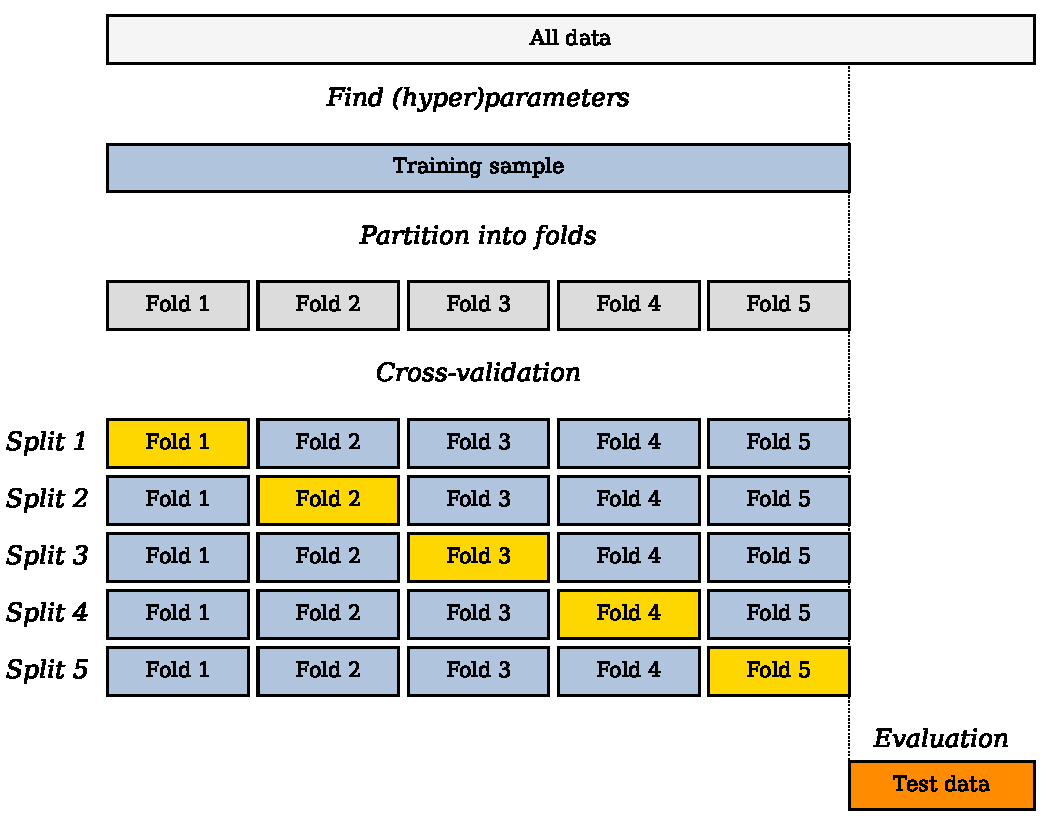
\includegraphics{images/cv_split.pdf}
\end{adjustbox}
\caption{CV split}
\end{figure}

    In this unit we will skip the final step of assessing generalisability
on the test data set. Consequently, when running cross-validation, we
will only use training/validation data sets and we will use the terms
``validation'' and ``test'' interchangeably.

The \texttt{scikit-learn}
\href{https://scikit-learn.org/stable/modules/cross_validation.html}{documentation}
contains a wealth of additional information on cross-validation. Another
method to perform hyperparameter tuning is
\href{https://scikit-learn.org/stable/modules/grid_search.html}{grid
search} which we won't cover in this unit.

    \hypertarget{example-tuning-of-the-polynomial-degree}{%
\vspace{1em}\subsubsection{Example: Tuning of the polynomial
degree}\label{example-tuning-of-the-polynomial-degree}}

To illustrate the concept, we demonstrate the procedure outlined above
by tuning the polynomial degree for the example covered in the previous
section by minimising the root mean squared error (RMSE).

We recreate the data set in the same way as before, using
\texttt{LivingArea} and \texttt{LotArea} as explanatory variables.

    \begin{tcolorbox}[breakable, size=fbox, boxrule=1pt, pad at break*=1mm,colback=cellbackground, colframe=cellborder]
\prompt{In}{incolor}{27}{\boxspacing}
\begin{Verbatim}[commandchars=\\\{\}]
\PY{k+kn}{import} \PY{n+nn}{pandas} \PY{k}{as} \PY{n+nn}{pd}

\PY{n}{df} \PY{o}{=} \PY{n}{pd}\PY{o}{.}\PY{n}{read\PYZus{}csv}\PY{p}{(}\PY{l+s+sa}{f}\PY{l+s+s1}{\PYZsq{}}\PY{l+s+si}{\PYZob{}}\PY{n}{DATA\PYZus{}PATH}\PY{l+s+si}{\PYZcb{}}\PY{l+s+s1}{/ames\PYZus{}houses.csv}\PY{l+s+s1}{\PYZsq{}}\PY{p}{)}

\PY{n}{features} \PY{o}{=} \PY{p}{[}\PY{l+s+s1}{\PYZsq{}}\PY{l+s+s1}{LivingArea}\PY{l+s+s1}{\PYZsq{}}\PY{p}{,} \PY{l+s+s1}{\PYZsq{}}\PY{l+s+s1}{LotArea}\PY{l+s+s1}{\PYZsq{}}\PY{p}{]}
\PY{n}{target} \PY{o}{=} \PY{l+s+s1}{\PYZsq{}}\PY{l+s+s1}{SalePrice}\PY{l+s+s1}{\PYZsq{}}

\PY{n}{y} \PY{o}{=} \PY{n}{df}\PY{p}{[}\PY{n}{target}\PY{p}{]}\PY{o}{.}\PY{n}{to\PYZus{}numpy}\PY{p}{(}\PY{p}{)}
\PY{n}{X} \PY{o}{=} \PY{n}{df}\PY{p}{[}\PY{n}{features}\PY{p}{]}\PY{o}{.}\PY{n}{to\PYZus{}numpy}\PY{p}{(}\PY{p}{)}
\end{Verbatim}
\end{tcolorbox}

    We now iterate over the candidate polynomial degrees \(d = 0,\dots,4\)
and apply \(k\)-fold cross-validation with 10 folds. There is no need to
manually split the sample into training and validation/test sub-sets.
Instead, we use the
\href{https://scikit-learn.org/stable/modules/generated/sklearn.model_selection.KFold.html\#sklearn.model_selection.KFold}{\texttt{KFold}}
class to automatically create the splits for us. Once we have created an
instance with the desired number of folds, \eg
\texttt{KFold(n\_splits=10)}, we can call the \texttt{split()} method
which iterates trough all possible combinations of training and test
data sets and returns the array indices for each.

    \begin{tcolorbox}[breakable, size=fbox, boxrule=1pt, pad at break*=1mm,colback=cellbackground, colframe=cellborder]
\prompt{In}{incolor}{28}{\boxspacing}
\begin{Verbatim}[commandchars=\\\{\}]
\PY{k+kn}{from} \PY{n+nn}{sklearn}\PY{n+nn}{.}\PY{n+nn}{pipeline} \PY{k+kn}{import} \PY{n}{Pipeline}
\PY{k+kn}{from} \PY{n+nn}{sklearn}\PY{n+nn}{.}\PY{n+nn}{preprocessing} \PY{k+kn}{import} \PY{n}{PolynomialFeatures}
\PY{k+kn}{from} \PY{n+nn}{sklearn}\PY{n+nn}{.}\PY{n+nn}{linear\PYZus{}model} \PY{k+kn}{import} \PY{n}{LinearRegression}
\PY{k+kn}{from} \PY{n+nn}{sklearn}\PY{n+nn}{.}\PY{n+nn}{model\PYZus{}selection} \PY{k+kn}{import} \PY{n}{KFold}
\PY{k+kn}{from} \PY{n+nn}{sklearn}\PY{n+nn}{.}\PY{n+nn}{metrics} \PY{k+kn}{import} \PY{n}{mean\PYZus{}squared\PYZus{}error}

\PY{n}{degrees} \PY{o}{=} \PY{n}{np}\PY{o}{.}\PY{n}{arange}\PY{p}{(}\PY{l+m+mi}{5}\PY{p}{)}

\PY{n}{rmse\PYZus{}mean} \PY{o}{=} \PY{p}{[}\PY{p}{]}

\PY{k}{for} \PY{n}{d} \PY{o+ow}{in} \PY{n}{degrees}\PY{p}{:}

    \PY{c+c1}{\PYZsh{} Create pipeline to transform and fit the model. Pipeline depends}
    \PY{c+c1}{\PYZsh{} on polynomial degree!}
    \PY{n}{pipe} \PY{o}{=} \PY{n}{Pipeline}\PY{p}{(}\PY{n}{steps}\PY{o}{=}\PY{p}{[}
        \PY{p}{(}\PY{l+s+s1}{\PYZsq{}}\PY{l+s+s1}{poly}\PY{l+s+s1}{\PYZsq{}}\PY{p}{,} \PY{n}{PolynomialFeatures}\PY{p}{(}\PY{n}{degree}\PY{o}{=}\PY{n}{d}\PY{p}{,} \PY{n}{include\PYZus{}bias}\PY{o}{=}\PY{k+kc}{True}\PY{p}{)}\PY{p}{)}\PY{p}{,}
        \PY{p}{(}\PY{l+s+s1}{\PYZsq{}}\PY{l+s+s1}{lr}\PY{l+s+s1}{\PYZsq{}}\PY{p}{,} \PY{n}{LinearRegression}\PY{p}{(}\PY{n}{fit\PYZus{}intercept}\PY{o}{=}\PY{k+kc}{False}\PY{p}{)}\PY{p}{)}
    \PY{p}{]}\PY{p}{)}

    \PY{n}{rmse\PYZus{}fold} \PY{o}{=} \PY{p}{[}\PY{p}{]}

    \PY{c+c1}{\PYZsh{} Create 10 folds}
    \PY{n}{folds} \PY{o}{=} \PY{n}{KFold}\PY{p}{(}\PY{n}{n\PYZus{}splits}\PY{o}{=}\PY{l+m+mi}{10}\PY{p}{)}

    \PY{c+c1}{\PYZsh{} Iterate through all combinations of training/test data}
    \PY{k}{for} \PY{n}{itrain}\PY{p}{,} \PY{n}{itest} \PY{o+ow}{in} \PY{n}{folds}\PY{o}{.}\PY{n}{split}\PY{p}{(}\PY{n}{X}\PY{p}{,} \PY{n}{y}\PY{p}{)}\PY{p}{:}

        \PY{c+c1}{\PYZsh{} Extract training data for this split}
        \PY{n}{X\PYZus{}train} \PY{o}{=} \PY{n}{X}\PY{p}{[}\PY{n}{itrain}\PY{p}{]}
        \PY{n}{y\PYZus{}train} \PY{o}{=} \PY{n}{y}\PY{p}{[}\PY{n}{itrain}\PY{p}{]}

        \PY{c+c1}{\PYZsh{} Extract test (or validation) data for this split}
        \PY{n}{X\PYZus{}test} \PY{o}{=} \PY{n}{X}\PY{p}{[}\PY{n}{itest}\PY{p}{]}
        \PY{n}{y\PYZus{}test} \PY{o}{=} \PY{n}{y}\PY{p}{[}\PY{n}{itest}\PY{p}{]}

        \PY{c+c1}{\PYZsh{} Fit model on training data for given degree}
        \PY{n}{pipe}\PY{o}{.}\PY{n}{fit}\PY{p}{(}\PY{n}{X\PYZus{}train}\PY{p}{,} \PY{n}{y\PYZus{}train}\PY{p}{)}

        \PY{c+c1}{\PYZsh{} Predict response on test data}
        \PY{n}{y\PYZus{}test\PYZus{}hat} \PY{o}{=} \PY{n}{pipe}\PY{o}{.}\PY{n}{predict}\PY{p}{(}\PY{n}{X\PYZus{}test}\PY{p}{)}

        \PY{c+c1}{\PYZsh{} Compute RMSE as model fit measure: function returns RMSE }
        \PY{c+c1}{\PYZsh{} if squared=False is passed!}
        \PY{n}{rmse} \PY{o}{=} \PY{n}{mean\PYZus{}squared\PYZus{}error}\PY{p}{(}\PY{n}{y\PYZus{}test}\PY{p}{,} \PY{n}{y\PYZus{}test\PYZus{}hat}\PY{p}{,} \PY{n}{squared}\PY{o}{=}\PY{k+kc}{False}\PY{p}{)}

        \PY{c+c1}{\PYZsh{} Store RMSE for current split}
        \PY{n}{rmse\PYZus{}fold}\PY{o}{.}\PY{n}{append}\PY{p}{(}\PY{n}{rmse}\PY{p}{)}

    \PY{c+c1}{\PYZsh{} Store average MSE for current polynomial degree}
    \PY{n}{rmse\PYZus{}mean}\PY{o}{.}\PY{n}{append}\PY{p}{(}\PY{n}{np}\PY{o}{.}\PY{n}{mean}\PY{p}{(}\PY{n}{rmse\PYZus{}fold}\PY{p}{)}\PY{p}{)}
    
\PY{c+c1}{\PYZsh{} Convert to NumPy array}
\PY{n}{rmse\PYZus{}mean} \PY{o}{=} \PY{n}{np}\PY{o}{.}\PY{n}{array}\PY{p}{(}\PY{n}{rmse\PYZus{}mean}\PY{p}{)}

\PY{c+c1}{\PYZsh{} Print average RMSE for all polynomial degrees}
\PY{n}{rmse\PYZus{}mean}
\end{Verbatim}
\end{tcolorbox}

            \begin{tcolorbox}[breakable, size=fbox, boxrule=.5pt, pad at break*=1mm, opacityfill=0]
\prompt{Out}{outcolor}{28}{\boxspacing}
\begin{Verbatim}[commandchars=\\\{\}]
array([ 79020.25214052,  55268.49840787,  55228.58262438,  55885.05422781,
       437077.00283378])
\end{Verbatim}
\end{tcolorbox}
        
    This code returns an array of 5 averaged RMSEs, one for each
\(d = 0, \dots, 4\). We can now find the optimal \(d\) by picking the
one which has the lowest mean squared error in the test samples using
the
\href{https://numpy.org/doc/stable/reference/generated/numpy.argmin.html}{\texttt{argmin()}}
function which returns the \emph{index} of the smallest array element.

    \begin{tcolorbox}[breakable, size=fbox, boxrule=1pt, pad at break*=1mm,colback=cellbackground, colframe=cellborder]
\prompt{In}{incolor}{29}{\boxspacing}
\begin{Verbatim}[commandchars=\\\{\}]
\PY{c+c1}{\PYZsh{} Find index of polynomial degree with smallest RMSE}
\PY{n}{imin} \PY{o}{=} \PY{n}{np}\PY{o}{.}\PY{n}{argmin}\PY{p}{(}\PY{n}{rmse\PYZus{}mean}\PY{p}{)}

\PY{c+c1}{\PYZsh{} RMSE\PYZhy{}minimising degree}
\PY{n}{dmin} \PY{o}{=} \PY{n}{degrees}\PY{p}{[}\PY{n}{imin}\PY{p}{]}

\PY{n+nb}{print}\PY{p}{(}\PY{l+s+sa}{f}\PY{l+s+s1}{\PYZsq{}}\PY{l+s+s1}{Polynomial degree with minimum RMSE: }\PY{l+s+si}{\PYZob{}}\PY{n}{dmin}\PY{l+s+si}{\PYZcb{}}\PY{l+s+s1}{\PYZsq{}}\PY{p}{)}
\end{Verbatim}
\end{tcolorbox}

    \begin{Verbatim}[commandchars=\\\{\}]
Polynomial degree with minimum RMSE: 2
    \end{Verbatim}

    Finally, it is often instructive to visualise how the RMSE evolves as a
function of the hyperparameter we want to tune.

    \begin{tcolorbox}[breakable, size=fbox, boxrule=1pt, pad at break*=1mm,colback=cellbackground, colframe=cellborder]
\prompt{In}{incolor}{30}{\boxspacing}
\begin{Verbatim}[commandchars=\\\{\}]
\PY{n}{plt}\PY{o}{.}\PY{n}{plot}\PY{p}{(}\PY{n}{degrees}\PY{p}{,} \PY{n}{rmse\PYZus{}mean}\PY{p}{,} \PY{n}{marker}\PY{o}{=}\PY{l+s+s1}{\PYZsq{}}\PY{l+s+s1}{o}\PY{l+s+s1}{\PYZsq{}}\PY{p}{,} \PY{n}{ms}\PY{o}{=}\PY{l+m+mi}{3}\PY{p}{)}
\PY{n}{plt}\PY{o}{.}\PY{n}{xlabel}\PY{p}{(}\PY{l+s+s1}{\PYZsq{}}\PY{l+s+s1}{Polynomial degree}\PY{l+s+s1}{\PYZsq{}}\PY{p}{)}
\PY{n}{plt}\PY{o}{.}\PY{n}{ylabel}\PY{p}{(}\PY{l+s+s1}{\PYZsq{}}\PY{l+s+s1}{Cross\PYZhy{}validated RMSE}\PY{l+s+s1}{\PYZsq{}}\PY{p}{)}
\PY{n}{plt}\PY{o}{.}\PY{n}{scatter}\PY{p}{(}\PY{n}{degrees}\PY{p}{[}\PY{n}{imin}\PY{p}{]}\PY{p}{,} \PY{n}{rmse\PYZus{}mean}\PY{p}{[}\PY{n}{imin}\PY{p}{]}\PY{p}{,} \PY{n}{s}\PY{o}{=}\PY{l+m+mi}{15}\PY{p}{,} \PY{n}{c}\PY{o}{=}\PY{l+s+s1}{\PYZsq{}}\PY{l+s+s1}{black}\PY{l+s+s1}{\PYZsq{}}\PY{p}{,} \PY{n}{zorder}\PY{o}{=}\PY{l+m+mi}{100}\PY{p}{)}
\PY{n}{plt}\PY{o}{.}\PY{n}{xticks}\PY{p}{(}\PY{n}{degrees}\PY{p}{)}
\PY{n}{plt}\PY{o}{.}\PY{n}{axvline}\PY{p}{(}\PY{n}{imin}\PY{p}{,} \PY{n}{ls}\PY{o}{=}\PY{l+s+s1}{\PYZsq{}}\PY{l+s+s1}{:}\PY{l+s+s1}{\PYZsq{}}\PY{p}{,} \PY{n}{lw}\PY{o}{=}\PY{l+m+mf}{0.75}\PY{p}{,} \PY{n}{c}\PY{o}{=}\PY{l+s+s1}{\PYZsq{}}\PY{l+s+s1}{black}\PY{l+s+s1}{\PYZsq{}}\PY{p}{)}
\end{Verbatim}
\end{tcolorbox}

            \begin{tcolorbox}[breakable, size=fbox, boxrule=.5pt, pad at break*=1mm, opacityfill=0]
\prompt{Out}{outcolor}{30}{\boxspacing}
\begin{Verbatim}[commandchars=\\\{\}]
<matplotlib.lines.Line2D at 0x7fca84770070>
\end{Verbatim}
\end{tcolorbox}
        
    \begin{center}
    \adjustimage{max size={0.9\linewidth}{0.9\paperheight}}{unit10_files/unit10_69_1.pdf}
    \end{center}
    
    Here we see that for \(d=0\) (the intercept-only model), the model
underfits the data leading to a high prediction error. However, higher
\(d\)'s do not always translate into a better fit. For \(d = 4\), the
model vastly overfits the data, resulting in poor performance in the
test sample and a very large RMSE.

    \hypertarget{automating-cross-validation}{%
\subsubsection*{Automating
cross-validation}\label{automating-cross-validation}}

The code implemented above to run cross-validation was needlessly
complex even though we leveraged the \texttt{KFold} class to do the
sample splitting for us. Fortunately, \texttt{scikit-learn} provides us
with even more convenience functions that further simplify this process.
For example, if we want to perform tuning based on a single score (such
as the root mean squared error), we can instead use
\href{https://scikit-learn.org/stable/modules/generated/sklearn.model_selection.cross_val_score.html}{\texttt{cross\_val\_score()}}.
This function requires us to specify an estimator (or a pipeline), the
number of folds to use for cross-validation (\texttt{cv=10}) and the
metric to evaluate. For example, if we want to compute the RMSE, we
would pass the argument
\texttt{scoring=\textquotesingle{}neg\_root\_mean\_squared\_error\textquotesingle{}}.
Note that the function returns the \emph{negative} RMSE which we need to
correct manually.

See the
\href{https://scikit-learn.org/stable/modules/model_evaluation.html\#scoring-parameter}{documentation}
for a complete list of valid metrics that can be passed as
\texttt{scoring} arguments. Alternatively, \texttt{scikit-learn} lists
available metrics by running

\begin{Shaded}
\begin{Highlighting}[]
\ImportTok{import}\NormalTok{ sklearn.metrics}
\NormalTok{sklearn.metrics.get\_scorer\_names()}
\end{Highlighting}
\end{Shaded}

The following code re-implements the k-fold cross-validation from
earlier using \texttt{cross\_val\_score()}:

    \begin{tcolorbox}[breakable, size=fbox, boxrule=1pt, pad at break*=1mm,colback=cellbackground, colframe=cellborder]
\prompt{In}{incolor}{31}{\boxspacing}
\begin{Verbatim}[commandchars=\\\{\}]
\PY{k+kn}{from} \PY{n+nn}{sklearn}\PY{n+nn}{.}\PY{n+nn}{model\PYZus{}selection} \PY{k+kn}{import} \PY{n}{cross\PYZus{}val\PYZus{}score}

\PY{n}{degrees} \PY{o}{=} \PY{n}{np}\PY{o}{.}\PY{n}{arange}\PY{p}{(}\PY{l+m+mi}{5}\PY{p}{)}

\PY{n}{rmse\PYZus{}mean} \PY{o}{=} \PY{p}{[}\PY{p}{]}
\PY{n}{rmse\PYZus{}std} \PY{o}{=} \PY{p}{[}\PY{p}{]}

\PY{k}{for} \PY{n}{d} \PY{o+ow}{in} \PY{n}{degrees}\PY{p}{:}

    \PY{n}{pipe} \PY{o}{=} \PY{n}{Pipeline}\PY{p}{(}\PY{n}{steps}\PY{o}{=}\PY{p}{[}
        \PY{p}{(}\PY{l+s+s1}{\PYZsq{}}\PY{l+s+s1}{poly}\PY{l+s+s1}{\PYZsq{}}\PY{p}{,} \PY{n}{PolynomialFeatures}\PY{p}{(}\PY{n}{degree}\PY{o}{=}\PY{n}{d}\PY{p}{,} \PY{n}{include\PYZus{}bias}\PY{o}{=}\PY{k+kc}{True}\PY{p}{)}\PY{p}{)}\PY{p}{,}
        \PY{p}{(}\PY{l+s+s1}{\PYZsq{}}\PY{l+s+s1}{lr}\PY{l+s+s1}{\PYZsq{}}\PY{p}{,} \PY{n}{LinearRegression}\PY{p}{(}\PY{n}{fit\PYZus{}intercept}\PY{o}{=}\PY{k+kc}{False}\PY{p}{)}\PY{p}{)}
    \PY{p}{]}\PY{p}{)}

    \PY{n}{score} \PY{o}{=} \PY{n}{cross\PYZus{}val\PYZus{}score}\PY{p}{(}
        \PY{n}{pipe}\PY{p}{,} 
        \PY{n}{X}\PY{p}{,} \PY{n}{y}\PY{p}{,} 
        \PY{n}{scoring}\PY{o}{=}\PY{l+s+s1}{\PYZsq{}}\PY{l+s+s1}{neg\PYZus{}root\PYZus{}mean\PYZus{}squared\PYZus{}error}\PY{l+s+s1}{\PYZsq{}}\PY{p}{,} 
        \PY{n}{cv}\PY{o}{=}\PY{l+m+mi}{10}
    \PY{p}{)}

    \PY{c+c1}{\PYZsh{} Function returns NEGATIVE RMSE, correct this here!}
    \PY{n}{rmse\PYZus{}mean}\PY{o}{.}\PY{n}{append}\PY{p}{(}\PY{n}{np}\PY{o}{.}\PY{n}{mean}\PY{p}{(}\PY{o}{\PYZhy{}}\PY{n}{score}\PY{p}{)}\PY{p}{)}
    
\PY{c+c1}{\PYZsh{} Convert to NumPy array}
\PY{n}{rmse\PYZus{}mean} \PY{o}{=} \PY{n}{np}\PY{o}{.}\PY{n}{array}\PY{p}{(}\PY{n}{rmse\PYZus{}mean}\PY{p}{)}

\PY{c+c1}{\PYZsh{} Print average RMSE for all polynomial degrees}
\PY{n}{rmse\PYZus{}mean}
\end{Verbatim}
\end{tcolorbox}

            \begin{tcolorbox}[breakable, size=fbox, boxrule=.5pt, pad at break*=1mm, opacityfill=0]
\prompt{Out}{outcolor}{31}{\boxspacing}
\begin{Verbatim}[commandchars=\\\{\}]
array([ 79020.25214052,  55268.49840787,  55228.58262438,  55885.05422781,
       437077.00283378])
\end{Verbatim}
\end{tcolorbox}
        
    The RMSE-minimising degree is of course the same as before:

    \begin{tcolorbox}[breakable, size=fbox, boxrule=1pt, pad at break*=1mm,colback=cellbackground, colframe=cellborder]
\prompt{In}{incolor}{32}{\boxspacing}
\begin{Verbatim}[commandchars=\\\{\}]
\PY{n}{imin} \PY{o}{=} \PY{n}{np}\PY{o}{.}\PY{n}{argmin}\PY{p}{(}\PY{n}{rmse\PYZus{}mean}\PY{p}{)}
\PY{n}{dmin} \PY{o}{=} \PY{n}{degrees}\PY{p}{[}\PY{n}{imin}\PY{p}{]}

\PY{n+nb}{print}\PY{p}{(}\PY{l+s+sa}{f}\PY{l+s+s1}{\PYZsq{}}\PY{l+s+s1}{Polynomial degree with min. RMSE: }\PY{l+s+si}{\PYZob{}}\PY{n}{dmin}\PY{l+s+si}{\PYZcb{}}\PY{l+s+s1}{\PYZsq{}}\PY{p}{)}
\end{Verbatim}
\end{tcolorbox}

    \begin{Verbatim}[commandchars=\\\{\}]
Polynomial degree with min. RMSE: 2
    \end{Verbatim}


\hypertarget{linear-models-with-regularisation-ridge-regression}{%
\subsection{Linear models with regularisation: Ridge
regression}\label{linear-models-with-regularisation-ridge-regression}}

The linear models we encountered so far are part of the standard
econometrics toolbox. In this section, we look at extensions that make
these models more useful for machine learning applications.

The first model we study is Ridge regression, which estimates a linear
model but adds a penalty term to the loss function which is now given by
\[
L(\mu, \bm\beta) = 
    \underbrace{\sum_{i=1}^N \Bigl(
    y_i - \mu - \mathbf{x}_i'\bm\beta\Bigr)^2}_{\text{Sum of squared errors}}
    + 
    \underbrace{\alpha \sum_{k=1}^K\beta_k^2}_{\text{L2 penalty}}
\] Compared to ordinary least squares (OLS) we discussed initially, the
penalty term increases the loss function if the estimated coefficients
\(\bm\beta\) are large. This term is called an L2 penalty because
it corresponds to the (squared) L2 vector norm. In many textbooks, you
will see the penalty term written as \(\alpha \|\bm\beta\|_2^2\)
which is equivalent to the formula used above.

For any \(\alpha > 0\), the loss function is increasing in the
(absolute) coefficient values, thus the minimum \(L\) might be one where
the elements of \(\bm\beta\) are smaller than what they would have
been with OLS. We therefore say that that Ridge regression applies
\emph{regularisation} or \emph{shrinkage}. Note, however, that the
intercept which we now denote by \(\mu\) is not included in the penalty
term, and thus no regularisation is applied to it.

Clearly, the regularisation strength depends on the value of \(\alpha\).
For tiny (or zero) \(\alpha\), the estimated
\(\widehat{\bm\beta}\) will be close (or identical) to OLS, while
for large \(\alpha\) the estimated coefficients will be compressed
towards zero. In this setting, \(\alpha\) is a hyperparameter and we can
accordingly use cross-validation to find an ``optimal'' value.

Why would we ever want to use Ridge regression given that OLS is the
best linear unbiased estimator? It turns out that regularisation can
help in scenarios where we have a large number of (potentially
multicollinear) regressors in which case OLS is prone to overfitting.

    \hypertarget{example-polynomial-approximation}{%
\vspace{1em}\subsubsection{Example: Polynomial
approximation}\label{example-polynomial-approximation}}

We illustrate such problems and the benefits of Ridge regression using a
highly stylised example. Imagine we want to approximate a non-linear
function using a high-order polynomial, a setting which is notoriously
susceptible to overfitting (also see the optional exercises for more
illustrations). Assume that our model is given by \[
\begin{aligned}
y_i &= \cos\left( \frac{3}{2}\pi x_i \right) + \epsilon_i \\
    \epsilon &\stackrel{\text{iid}}{\sim} N(0, 0.25)
\end{aligned}
\] where \(\epsilon_i\) as an additive, normally-distributed measurement
error term with mean \(0\) and variance \(\frac{1}{4}\).

The true values of \(y\) (without measurement error) are computed using
the function \texttt{compute\_true\_y()} which returns \(y\) for a given
\(x\).

    \begin{tcolorbox}[breakable, size=fbox, boxrule=1pt, pad at break*=1mm,colback=cellbackground, colframe=cellborder]
\prompt{In}{incolor}{33}{\boxspacing}
\begin{Verbatim}[commandchars=\\\{\}]
\PY{k+kn}{import} \PY{n+nn}{numpy} \PY{k}{as} \PY{n+nn}{np}

\PY{c+c1}{\PYZsh{} True function (w/o errors)}
\PY{k}{def} \PY{n+nf}{compute\PYZus{}true\PYZus{}y}\PY{p}{(}\PY{n}{x}\PY{p}{)}\PY{p}{:}
    \PY{k}{return} \PY{n}{np}\PY{o}{.}\PY{n}{cos}\PY{p}{(}\PY{l+m+mf}{1.5} \PY{o}{*} \PY{n}{np}\PY{o}{.}\PY{n}{pi} \PY{o}{*} \PY{n}{x}\PY{p}{)}
\end{Verbatim}
\end{tcolorbox}

    The following code creates a demo sample with \(N=100\) observations.

    \begin{tcolorbox}[breakable, size=fbox, boxrule=1pt, pad at break*=1mm,colback=cellbackground, colframe=cellborder]
\prompt{In}{incolor}{34}{\boxspacing}
\begin{Verbatim}[commandchars=\\\{\}]
\PY{k+kn}{from} \PY{n+nn}{numpy}\PY{n+nn}{.}\PY{n+nn}{random} \PY{k+kn}{import} \PY{n}{default\PYZus{}rng}

\PY{c+c1}{\PYZsh{} Initialise random number generator}
\PY{n}{rng} \PY{o}{=} \PY{n}{default\PYZus{}rng}\PY{p}{(}\PY{l+m+mi}{1234}\PY{p}{)}

\PY{c+c1}{\PYZsh{} Sample size}
\PY{n}{N} \PY{o}{=} \PY{l+m+mi}{100}

\PY{c+c1}{\PYZsh{} Randomly draw explanatory variable x uniformly distributed on [0, 1]}
\PY{n}{x} \PY{o}{=} \PY{n}{rng}\PY{o}{.}\PY{n}{random}\PY{p}{(}\PY{n}{size}\PY{o}{=}\PY{n}{N}\PY{p}{)}

\PY{c+c1}{\PYZsh{} Draw errors from normal distribution}
\PY{n}{epsilon} \PY{o}{=} \PY{n}{rng}\PY{o}{.}\PY{n}{normal}\PY{p}{(}\PY{n}{scale}\PY{o}{=}\PY{l+m+mf}{0.5}\PY{p}{,} \PY{n}{size}\PY{o}{=}\PY{n}{N}\PY{p}{)}

\PY{c+c1}{\PYZsh{} Compute y, add measurement error}
\PY{n}{y} \PY{o}{=} \PY{n}{compute\PYZus{}true\PYZus{}y}\PY{p}{(}\PY{n}{x}\PY{p}{)} \PY{o}{+} \PY{n}{epsilon}
\end{Verbatim}
\end{tcolorbox}

    The next graph visualises the true relationship and the sample points
\((x_i, y_i)\).

    \begin{tcolorbox}[breakable, size=fbox, boxrule=1pt, pad at break*=1mm,colback=cellbackground, colframe=cellborder]
\prompt{In}{incolor}{35}{\boxspacing}
\begin{Verbatim}[commandchars=\\\{\}]
\PY{k+kn}{import} \PY{n+nn}{matplotlib}\PY{n+nn}{.}\PY{n+nn}{pyplot} \PY{k}{as} \PY{n+nn}{plt}

\PY{c+c1}{\PYZsh{} Sample scatter plot}
\PY{n}{plt}\PY{o}{.}\PY{n}{scatter}\PY{p}{(}\PY{n}{x}\PY{p}{,} \PY{n}{y}\PY{p}{,} \PY{n}{s}\PY{o}{=}\PY{l+m+mi}{20}\PY{p}{,} \PY{n}{color}\PY{o}{=}\PY{l+s+s1}{\PYZsq{}}\PY{l+s+s1}{none}\PY{l+s+s1}{\PYZsq{}}\PY{p}{,} \PY{n}{edgecolor}\PY{o}{=}\PY{l+s+s1}{\PYZsq{}}\PY{l+s+s1}{steelblue}\PY{l+s+s1}{\PYZsq{}}\PY{p}{,} 
    \PY{n}{lw}\PY{o}{=}\PY{l+m+mf}{0.75}\PY{p}{,} \PY{n}{label}\PY{o}{=}\PY{l+s+s1}{\PYZsq{}}\PY{l+s+s1}{Sample}\PY{l+s+s1}{\PYZsq{}}\PY{p}{)}

\PY{c+c1}{\PYZsh{} Plot true relationship}
\PY{n}{xvalues} \PY{o}{=} \PY{n}{np}\PY{o}{.}\PY{n}{linspace}\PY{p}{(}\PY{l+m+mf}{0.0}\PY{p}{,} \PY{l+m+mf}{1.0}\PY{p}{,} \PY{l+m+mi}{101}\PY{p}{)}
\PY{n}{plt}\PY{o}{.}\PY{n}{plot}\PY{p}{(}\PY{n}{xvalues}\PY{p}{,} \PY{n}{compute\PYZus{}true\PYZus{}y}\PY{p}{(}\PY{n}{xvalues}\PY{p}{)}\PY{p}{,} \PY{n}{color}\PY{o}{=}\PY{l+s+s1}{\PYZsq{}}\PY{l+s+s1}{black}\PY{l+s+s1}{\PYZsq{}}\PY{p}{,} \PY{n}{lw}\PY{o}{=}\PY{l+m+mf}{1.0}\PY{p}{,} 
    \PY{n}{label}\PY{o}{=}\PY{l+s+s1}{\PYZsq{}}\PY{l+s+s1}{True function}\PY{l+s+s1}{\PYZsq{}}\PY{p}{)}

\PY{n}{plt}\PY{o}{.}\PY{n}{xlabel}\PY{p}{(}\PY{l+s+s1}{\PYZsq{}}\PY{l+s+s1}{\PYZdl{}x\PYZdl{}}\PY{l+s+s1}{\PYZsq{}}\PY{p}{)}
\PY{n}{plt}\PY{o}{.}\PY{n}{ylabel}\PY{p}{(}\PY{l+s+s1}{\PYZsq{}}\PY{l+s+s1}{\PYZdl{}y\PYZdl{}}\PY{l+s+s1}{\PYZsq{}}\PY{p}{)}
\end{Verbatim}
\end{tcolorbox}

            \begin{tcolorbox}[breakable, size=fbox, boxrule=.5pt, pad at break*=1mm, opacityfill=0]
\prompt{Out}{outcolor}{35}{\boxspacing}
\begin{Verbatim}[commandchars=\\\{\}]
Text(0, 0.5, '\$y\$')
\end{Verbatim}
\end{tcolorbox}
        
    \begin{center}
    \adjustimage{max size={0.9\linewidth}{0.9\paperheight}}{unit10_files/unit10_81_1.pdf}
    \end{center}
    
    \hypertarget{estimating-the-ridge-and-linear-regression-models}{%
\subsubsection*{Estimating the Ridge and linear regression
models}\label{estimating-the-ridge-and-linear-regression-models}}

We now estimate a polynomial approximation where we assume that \(y\) is
a degree-\(K\) polynomial in \(x\), \ie \[
y_i \approx \mu + \beta_1 x_i + \beta_2 x_i^2 + \cdots + \beta_K x_i^K 
\] For this example, we choose an unconventionally high \(K=15\) since
we anticipate that this leads to problems with OLS.

A few more steps are required before we can run the Ridge regression:

\begin{itemize}
\tightlist
\item
  We need to create the polynomial in \(x\) which we do with the
  \href{https://scikit-learn.org/stable/modules/generated/sklearn.preprocessing.PolynomialFeatures.html}{\texttt{PolynomialFeatures}}
  transformation we already encountered.
\item
  Moreover, regularisation methods can be susceptible to scaling issues,
  so we need to demean and normalise all input variables, \ie we make
  sure that each feature has mean \(0\) and a variance of \(1\). We can
  automate this step using the
  \href{https://scikit-learn.org/stable/modules/generated/sklearn.preprocessing.StandardScaler.html}{\texttt{StandardScaler}}
  transformation.
\item
  Finally, the estimation step is performed by the
  \href{https://scikit-learn.org/stable/modules/generated/sklearn.linear_model.Ridge.html}{\texttt{Ridge}}
  class.
\item
  We build a
  \href{https://scikit-learn.org/stable/modules/generated/sklearn.pipeline.Pipeline.html}{\texttt{Pipeline}}
  that combines these transformation together with the estimation step.
  We use the function
  \href{https://scikit-learn.org/stable/modules/generated/sklearn.pipeline.make_pipeline.html}{\texttt{make\_pipeline()}}
  to simplify this step.
\end{itemize}

To run the Ridge regression, we moreover need to specify the
regularisation strength \(\alpha\) which we set to \(\alpha = 3\) for
illustration.

    \begin{tcolorbox}[breakable, size=fbox, boxrule=1pt, pad at break*=1mm,colback=cellbackground, colframe=cellborder]
\prompt{In}{incolor}{36}{\boxspacing}
\begin{Verbatim}[commandchars=\\\{\}]
\PY{k+kn}{from} \PY{n+nn}{sklearn}\PY{n+nn}{.}\PY{n+nn}{linear\PYZus{}model} \PY{k+kn}{import} \PY{n}{Ridge}
\PY{k+kn}{from} \PY{n+nn}{sklearn}\PY{n+nn}{.}\PY{n+nn}{preprocessing} \PY{k+kn}{import} \PY{n}{PolynomialFeatures}\PY{p}{,} \PY{n}{StandardScaler}
\PY{k+kn}{from} \PY{n+nn}{sklearn}\PY{n+nn}{.}\PY{n+nn}{pipeline} \PY{k+kn}{import} \PY{n}{make\PYZus{}pipeline}

\PY{c+c1}{\PYZsh{} Polynomial degree}
\PY{n}{degree} \PY{o}{=} \PY{l+m+mi}{15}

\PY{c+c1}{\PYZsh{} Build pipeline of transformations and Ridge estimation.}
\PY{c+c1}{\PYZsh{} We create the polynomial transformation w/o the intercept so we }
\PY{c+c1}{\PYZsh{} need to include an intercept in the fitting step.}
\PY{n}{pipe\PYZus{}ridge} \PY{o}{=} \PY{n}{make\PYZus{}pipeline}\PY{p}{(}
    \PY{n}{PolynomialFeatures}\PY{p}{(}
        \PY{n}{degree}\PY{o}{=}\PY{n}{degree}\PY{p}{,} 
        \PY{n}{include\PYZus{}bias}\PY{o}{=}\PY{k+kc}{False}
    \PY{p}{)}\PY{p}{,}
    \PY{n}{StandardScaler}\PY{p}{(}\PY{p}{)}\PY{p}{,}                           \PY{c+c1}{\PYZsh{} standardise features}
    \PY{n}{Ridge}\PY{p}{(}\PY{n}{alpha}\PY{o}{=}\PY{l+m+mf}{3.0}\PY{p}{,} \PY{n}{fit\PYZus{}intercept}\PY{o}{=}\PY{k+kc}{True}\PY{p}{)}        \PY{c+c1}{\PYZsh{} Fit Ridge regression}
\PY{p}{)}

\PY{c+c1}{\PYZsh{} Make sure X is a matrix}
\PY{n}{X} \PY{o}{=} \PY{n}{x}\PY{p}{[}\PY{p}{:}\PY{p}{,} \PY{k+kc}{None}\PY{p}{]}

\PY{c+c1}{\PYZsh{} Fit model}
\PY{n}{pipe\PYZus{}ridge}\PY{o}{.}\PY{n}{fit}\PY{p}{(}\PY{n}{X}\PY{p}{,} \PY{n}{y}\PY{p}{)}
\end{Verbatim}
\end{tcolorbox}

            \begin{tcolorbox}[breakable, size=fbox, boxrule=.5pt, pad at break*=1mm, opacityfill=0]
\prompt{Out}{outcolor}{36}{\boxspacing}
\begin{Verbatim}[commandchars=\\\{\}]
Pipeline(steps=[('polynomialfeatures',
                 PolynomialFeatures(degree=15, include\_bias=False)),
                ('standardscaler', StandardScaler()),
                ('ridge', Ridge(alpha=3.0))])
\end{Verbatim}
\end{tcolorbox}
        
    It is instructive to estimate the same model using linear regression and
compare the results:

    \begin{tcolorbox}[breakable, size=fbox, boxrule=1pt, pad at break*=1mm,colback=cellbackground, colframe=cellborder]
\prompt{In}{incolor}{37}{\boxspacing}
\begin{Verbatim}[commandchars=\\\{\}]
\PY{k+kn}{from} \PY{n+nn}{sklearn}\PY{n+nn}{.}\PY{n+nn}{linear\PYZus{}model} \PY{k+kn}{import} \PY{n}{LinearRegression}

\PY{c+c1}{\PYZsh{} Create pipeline for linear model (linear regression does not require}
\PY{c+c1}{\PYZsh{} standardisation!)}
\PY{n}{pipe\PYZus{}lr} \PY{o}{=} \PY{n}{make\PYZus{}pipeline}\PY{p}{(}
    \PY{n}{PolynomialFeatures}\PY{p}{(}
        \PY{n}{degree}\PY{o}{=}\PY{n}{degree}\PY{p}{,} 
        \PY{n}{include\PYZus{}bias}\PY{o}{=}\PY{k+kc}{False}
    \PY{p}{)}\PY{p}{,}
    \PY{n}{LinearRegression}\PY{p}{(}\PY{n}{fit\PYZus{}intercept}\PY{o}{=}\PY{k+kc}{True}\PY{p}{)}
\PY{p}{)}

\PY{c+c1}{\PYZsh{} Make sure X is a matrix}
\PY{n}{X} \PY{o}{=} \PY{n}{x}\PY{p}{[}\PY{p}{:}\PY{p}{,} \PY{k+kc}{None}\PY{p}{]}

\PY{c+c1}{\PYZsh{} Fit model}
\PY{n}{pipe\PYZus{}lr}\PY{o}{.}\PY{n}{fit}\PY{p}{(}\PY{n}{X}\PY{p}{,} \PY{n}{y}\PY{p}{)}
\end{Verbatim}
\end{tcolorbox}

            \begin{tcolorbox}[breakable, size=fbox, boxrule=.5pt, pad at break*=1mm, opacityfill=0]
\prompt{Out}{outcolor}{37}{\boxspacing}
\begin{Verbatim}[commandchars=\\\{\}]
Pipeline(steps=[('polynomialfeatures',
                 PolynomialFeatures(degree=15, include\_bias=False)),
                ('linearregression', LinearRegression())])
\end{Verbatim}
\end{tcolorbox}
        
    To illustrate the difference for this artificial example, we add the
model predictions from the Ridge and linear regressions to the sample
scatter plot we created earlier.

    \begin{tcolorbox}[breakable, size=fbox, boxrule=1pt, pad at break*=1mm,colback=cellbackground, colframe=cellborder]
\prompt{In}{incolor}{38}{\boxspacing}
\begin{Verbatim}[commandchars=\\\{\}]
\PY{k+kn}{import} \PY{n+nn}{matplotlib}\PY{n+nn}{.}\PY{n+nn}{pyplot} \PY{k}{as} \PY{n+nn}{plt}

\PY{n}{fig}\PY{p}{,} \PY{n}{ax} \PY{o}{=} \PY{n}{plt}\PY{o}{.}\PY{n}{subplots}\PY{p}{(}\PY{l+m+mi}{1}\PY{p}{,} \PY{l+m+mi}{1}\PY{p}{,} \PY{n}{figsize}\PY{o}{=}\PY{p}{(}\PY{l+m+mi}{6}\PY{p}{,} \PY{l+m+mi}{4}\PY{p}{)}\PY{p}{)}

\PY{c+c1}{\PYZsh{} Grid on which to evaluate true model and predictions}
\PY{n}{xvalues} \PY{o}{=} \PY{n}{np}\PY{o}{.}\PY{n}{linspace}\PY{p}{(}\PY{n}{np}\PY{o}{.}\PY{n}{amin}\PY{p}{(}\PY{n}{x}\PY{p}{)}\PY{p}{,} \PY{n}{np}\PY{o}{.}\PY{n}{amax}\PY{p}{(}\PY{n}{x}\PY{p}{)}\PY{p}{,} \PY{l+m+mi}{500}\PY{p}{)}

\PY{c+c1}{\PYZsh{} Sample points scatter plot}
\PY{n}{ax}\PY{o}{.}\PY{n}{scatter}\PY{p}{(}\PY{n}{x}\PY{p}{,} \PY{n}{y}\PY{p}{,} \PY{n}{s}\PY{o}{=}\PY{l+m+mi}{20}\PY{p}{,} \PY{n}{color}\PY{o}{=}\PY{l+s+s1}{\PYZsq{}}\PY{l+s+s1}{none}\PY{l+s+s1}{\PYZsq{}}\PY{p}{,} \PY{n}{edgecolor}\PY{o}{=}\PY{l+s+s1}{\PYZsq{}}\PY{l+s+s1}{steelblue}\PY{l+s+s1}{\PYZsq{}}\PY{p}{,} 
    \PY{n}{lw}\PY{o}{=}\PY{l+m+mf}{0.75}\PY{p}{,} \PY{n}{alpha}\PY{o}{=}\PY{l+m+mf}{0.7}\PY{p}{,} \PY{n}{label}\PY{o}{=}\PY{l+s+s1}{\PYZsq{}}\PY{l+s+s1}{Sample}\PY{l+s+s1}{\PYZsq{}}\PY{p}{)}

\PY{c+c1}{\PYZsh{} True model}
\PY{n}{ax}\PY{o}{.}\PY{n}{plot}\PY{p}{(}\PY{n}{xvalues}\PY{p}{,} \PY{n}{compute\PYZus{}true\PYZus{}y}\PY{p}{(}\PY{n}{xvalues}\PY{p}{)}\PY{p}{,} \PY{n}{color}\PY{o}{=}\PY{l+s+s1}{\PYZsq{}}\PY{l+s+s1}{black}\PY{l+s+s1}{\PYZsq{}}\PY{p}{,} \PY{n}{lw}\PY{o}{=}\PY{l+m+mf}{1.0}\PY{p}{,} \PY{n}{alpha}\PY{o}{=}\PY{l+m+mf}{0.9}\PY{p}{,} 
    \PY{n}{label}\PY{o}{=}\PY{l+s+s1}{\PYZsq{}}\PY{l+s+s1}{True function}\PY{l+s+s1}{\PYZsq{}}\PY{p}{)}

\PY{c+c1}{\PYZsh{} LR prediction}
\PY{n}{ax}\PY{o}{.}\PY{n}{plot}\PY{p}{(}\PY{n}{xvalues}\PY{p}{,} \PY{n}{pipe\PYZus{}lr}\PY{o}{.}\PY{n}{predict}\PY{p}{(}\PY{n}{xvalues}\PY{p}{[}\PY{p}{:}\PY{p}{,} \PY{k+kc}{None}\PY{p}{]}\PY{p}{)}\PY{p}{,} \PY{n}{color}\PY{o}{=}\PY{l+s+s1}{\PYZsq{}}\PY{l+s+s1}{purple}\PY{l+s+s1}{\PYZsq{}}\PY{p}{,} 
    \PY{n}{alpha}\PY{o}{=}\PY{l+m+mf}{0.7}\PY{p}{,} \PY{n}{label}\PY{o}{=}\PY{l+s+s1}{\PYZsq{}}\PY{l+s+s1}{Linear regression}\PY{l+s+s1}{\PYZsq{}}\PY{p}{)}

\PY{c+c1}{\PYZsh{} Ridge prediction}
\PY{n}{ax}\PY{o}{.}\PY{n}{plot}\PY{p}{(}\PY{n}{xvalues}\PY{p}{,} \PY{n}{pipe\PYZus{}ridge}\PY{o}{.}\PY{n}{predict}\PY{p}{(}\PY{n}{xvalues}\PY{p}{[}\PY{p}{:}\PY{p}{,} \PY{k+kc}{None}\PY{p}{]}\PY{p}{)}\PY{p}{,} 
    \PY{n}{color}\PY{o}{=}\PY{l+s+s1}{\PYZsq{}}\PY{l+s+s1}{darkorange}\PY{l+s+s1}{\PYZsq{}}\PY{p}{,} \PY{n}{lw}\PY{o}{=}\PY{l+m+mf}{2.0}\PY{p}{,} 
    \PY{n}{label}\PY{o}{=}\PY{l+s+s1}{\PYZsq{}}\PY{l+s+s1}{Ridge}\PY{l+s+s1}{\PYZsq{}}
\PY{p}{)}
\PY{n}{ax}\PY{o}{.}\PY{n}{legend}\PY{p}{(}\PY{p}{)}
\PY{n}{ax}\PY{o}{.}\PY{n}{set\PYZus{}xlabel}\PY{p}{(}\PY{l+s+s1}{\PYZsq{}}\PY{l+s+s1}{\PYZdl{}x\PYZdl{}}\PY{l+s+s1}{\PYZsq{}}\PY{p}{)}
\PY{n}{ax}\PY{o}{.}\PY{n}{set\PYZus{}ylabel}\PY{p}{(}\PY{l+s+s1}{\PYZsq{}}\PY{l+s+s1}{\PYZdl{}y\PYZdl{}, \PYZdl{}}\PY{l+s+s1}{\PYZbs{}}\PY{l+s+s1}{widehat}\PY{l+s+si}{\PYZob{}y\PYZcb{}}\PY{l+s+s1}{\PYZdl{}}\PY{l+s+s1}{\PYZsq{}}\PY{p}{)}
\end{Verbatim}
\end{tcolorbox}

            \begin{tcolorbox}[breakable, size=fbox, boxrule=.5pt, pad at break*=1mm, opacityfill=0]
\prompt{Out}{outcolor}{38}{\boxspacing}
\begin{Verbatim}[commandchars=\\\{\}]
Text(0, 0.5, '\$y\$, \$\textbackslash{}\textbackslash{}widehat\{y\}\$')
\end{Verbatim}
\end{tcolorbox}
        
    \begin{center}
    \adjustimage{max size={0.9\linewidth}{0.9\paperheight}}{unit10_files/unit10_87_1.pdf}
    \end{center}
    
    As the graph shows, the OLS model vastly overfits the data which is what
we would expect in this settings. Conversely, the prediction of the
Ridge regression is reasonably close to the true function and much
better behaved despite the high polynomial degree used here.

To gain some intuition for what is going on, it is instructive to plot
the estimated Ridge coefficients for a whole range of \(\alpha\) values
which we do in the code below. Note that we choose the grid of
\(\alpha\) to be uniformly spaced in logs since we want to zoom in on
what happens when \(\alpha\) is small. This is accomplished by using
\href{https://numpy.org/doc/stable/reference/generated/numpy.logspace.html}{\texttt{np.logspace()}}
instead of \texttt{np.linspace()}.

    \begin{tcolorbox}[breakable, size=fbox, boxrule=1pt, pad at break*=1mm,colback=cellbackground, colframe=cellborder]
\prompt{In}{incolor}{39}{\boxspacing}
\begin{Verbatim}[commandchars=\\\{\}]
\PY{c+c1}{\PYZsh{} Create grid of alphas spaced uniformly in logs}
\PY{n}{alphas} \PY{o}{=} \PY{n}{np}\PY{o}{.}\PY{n}{logspace}\PY{p}{(}\PY{n}{start}\PY{o}{=}\PY{n}{np}\PY{o}{.}\PY{n}{log10}\PY{p}{(}\PY{l+m+mf}{5.0e\PYZhy{}3}\PY{p}{)}\PY{p}{,} \PY{n}{stop}\PY{o}{=}\PY{n}{np}\PY{o}{.}\PY{n}{log10}\PY{p}{(}\PY{l+m+mf}{1000.0}\PY{p}{)}\PY{p}{,} \PY{n}{num}\PY{o}{=}\PY{l+m+mi}{100}\PY{p}{)}

\PY{c+c1}{\PYZsh{} Re\PYZhy{}create pipeline w/o Ridge estimator, estimation step differs for each alpha}
\PY{n}{transform} \PY{o}{=} \PY{n}{make\PYZus{}pipeline}\PY{p}{(}
    \PY{n}{PolynomialFeatures}\PY{p}{(}
        \PY{n}{degree}\PY{o}{=}\PY{n}{degree}\PY{p}{,} 
        \PY{n}{include\PYZus{}bias}\PY{o}{=}\PY{k+kc}{False}
    \PY{p}{)}\PY{p}{,}
    \PY{n}{StandardScaler}\PY{p}{(}\PY{p}{)}
\PY{p}{)}

\PY{c+c1}{\PYZsh{} Create polynomial features}
\PY{n}{Xtrans} \PY{o}{=} \PY{n}{transform}\PY{o}{.}\PY{n}{fit\PYZus{}transform}\PY{p}{(}\PY{n}{x}\PY{p}{[}\PY{p}{:}\PY{p}{,} \PY{k+kc}{None}\PY{p}{]}\PY{p}{)}

\PY{c+c1}{\PYZsh{} Array to store coefficients for all alphas}
\PY{n}{coefs} \PY{o}{=} \PY{n}{np}\PY{o}{.}\PY{n}{empty}\PY{p}{(}\PY{p}{(}\PY{n+nb}{len}\PY{p}{(}\PY{n}{alphas}\PY{p}{)}\PY{p}{,} \PY{n}{Xtrans}\PY{o}{.}\PY{n}{shape}\PY{p}{[}\PY{l+m+mi}{1}\PY{p}{]}\PY{p}{)}\PY{p}{)}

\PY{c+c1}{\PYZsh{} Estimate Ridge for each alpha, store fitted coefficients}
\PY{k}{for} \PY{n}{i}\PY{p}{,} \PY{n}{alpha} \PY{o+ow}{in} \PY{n+nb}{enumerate}\PY{p}{(}\PY{n}{alphas}\PY{p}{)}\PY{p}{:}
    \PY{n}{ridge} \PY{o}{=} \PY{n}{Ridge}\PY{p}{(}\PY{n}{alpha}\PY{o}{=}\PY{n}{alpha}\PY{p}{,} \PY{n}{fit\PYZus{}intercept}\PY{o}{=}\PY{k+kc}{True}\PY{p}{)}
    
    \PY{c+c1}{\PYZsh{} Fit model for given alpha}
    \PY{n}{ridge}\PY{o}{.}\PY{n}{fit}\PY{p}{(}\PY{n}{Xtrans}\PY{p}{,} \PY{n}{y}\PY{p}{)}

    \PY{n}{coefs}\PY{p}{[}\PY{n}{i}\PY{p}{]} \PY{o}{=} \PY{n}{ridge}\PY{o}{.}\PY{n}{coef\PYZus{}}
\end{Verbatim}
\end{tcolorbox}

    The following plot shows each coefficient (one color corresponds to one
coefficients) for different values of \(\alpha\) on the \(x\)-axis. Note
that the \(x\)-axis is plotted on a \(\log_{10}\) scale which allows us
to zoom in on smaller values of \(\alpha\).

    \begin{tcolorbox}[breakable, size=fbox, boxrule=1pt, pad at break*=1mm,colback=cellbackground, colframe=cellborder]
\prompt{In}{incolor}{40}{\boxspacing}
\begin{Verbatim}[commandchars=\\\{\}]
\PY{n}{plt}\PY{o}{.}\PY{n}{figure}\PY{p}{(}\PY{n}{figsize}\PY{o}{=}\PY{p}{(}\PY{l+m+mi}{6}\PY{p}{,}\PY{l+m+mi}{4}\PY{p}{)}\PY{p}{)}
\PY{n}{plt}\PY{o}{.}\PY{n}{plot}\PY{p}{(}\PY{n}{alphas}\PY{p}{,} \PY{n}{coefs}\PY{p}{,} \PY{n}{lw}\PY{o}{=}\PY{l+m+mf}{1.0}\PY{p}{)}
\PY{n}{plt}\PY{o}{.}\PY{n}{xscale}\PY{p}{(}\PY{l+s+s1}{\PYZsq{}}\PY{l+s+s1}{log}\PY{l+s+s1}{\PYZsq{}}\PY{p}{,} \PY{n}{base}\PY{o}{=}\PY{l+m+mi}{10}\PY{p}{)}
\PY{n}{plt}\PY{o}{.}\PY{n}{axhline}\PY{p}{(}\PY{l+m+mf}{0.0}\PY{p}{,} \PY{n}{ls}\PY{o}{=}\PY{l+s+s1}{\PYZsq{}}\PY{l+s+s1}{\PYZhy{}\PYZhy{}}\PY{l+s+s1}{\PYZsq{}}\PY{p}{,} \PY{n}{lw}\PY{o}{=}\PY{l+m+mf}{0.75}\PY{p}{,} \PY{n}{c}\PY{o}{=}\PY{l+s+s1}{\PYZsq{}}\PY{l+s+s1}{black}\PY{l+s+s1}{\PYZsq{}}\PY{p}{)}
\PY{n}{plt}\PY{o}{.}\PY{n}{xlabel}\PY{p}{(}\PY{l+s+sa}{r}\PY{l+s+s1}{\PYZsq{}}\PY{l+s+s1}{Regularisation strength \PYZdl{}}\PY{l+s+s1}{\PYZbs{}}\PY{l+s+s1}{alpha\PYZdl{} (log scale)}\PY{l+s+s1}{\PYZsq{}}\PY{p}{)}
\PY{n}{plt}\PY{o}{.}\PY{n}{ylabel}\PY{p}{(}\PY{l+s+s1}{\PYZsq{}}\PY{l+s+s1}{Coefficient value}\PY{l+s+s1}{\PYZsq{}}\PY{p}{)}
\end{Verbatim}
\end{tcolorbox}

            \begin{tcolorbox}[breakable, size=fbox, boxrule=.5pt, pad at break*=1mm, opacityfill=0]
\prompt{Out}{outcolor}{40}{\boxspacing}
\begin{Verbatim}[commandchars=\\\{\}]
Text(0, 0.5, 'Coefficient value')
\end{Verbatim}
\end{tcolorbox}
        
    \begin{center}
    \adjustimage{max size={0.9\linewidth}{0.9\paperheight}}{unit10_files/unit10_91_1.pdf}
    \end{center}
    
    For small \(\alpha\) (on the left) the estimated coefficients are close
to the (standardised) OLS coefficients, but their values shrink towards
zero as \(\alpha\) increases. For a very large \(\alpha = 10^3\) the
estimated coefficients are basically zero since the penalty dominates
the sum of squared errors in the loss function.

    \hypertarget{tuning-the-regularisation-parameter-via-cross-validation}{%
\subsubsection{Tuning the regularisation parameter via
cross-validation}\label{tuning-the-regularisation-parameter-via-cross-validation}}

In the previous example, we picked an arbitrary regularisation strength
\(\alpha\) when fitting the Ridge regression. In applied work, we would
want to tune \(\alpha\) (which is a hyperparameter) using
cross-validation instead. To this end, we could use the generic
cross-validation functionality we studied earlier in this unit since
that one works for all types of estimators. However,
\texttt{scikit-learn} implements a cross-validation class specifically
for Ridge regression called
\href{https://scikit-learn.org/stable/modules/generated/sklearn.linear_model.RidgeCV.html}{\texttt{RidgeCV}}
which we use in the code below to find an optimal \(\alpha\).

    \begin{tcolorbox}[breakable, size=fbox, boxrule=1pt, pad at break*=1mm,colback=cellbackground, colframe=cellborder]
\prompt{In}{incolor}{41}{\boxspacing}
\begin{Verbatim}[commandchars=\\\{\}]
\PY{k+kn}{from} \PY{n+nn}{sklearn}\PY{n+nn}{.}\PY{n+nn}{linear\PYZus{}model} \PY{k+kn}{import} \PY{n}{RidgeCV}

\PY{c+c1}{\PYZsh{} RidgeCV does not support pipelines, so we need to transform x before}
\PY{c+c1}{\PYZsh{} cross\PYZhy{}validation.}
\PY{n}{transform} \PY{o}{=} \PY{n}{make\PYZus{}pipeline}\PY{p}{(}
    \PY{n}{PolynomialFeatures}\PY{p}{(}
        \PY{n}{degree}\PY{o}{=}\PY{n}{degree}\PY{p}{,} 
        \PY{n}{include\PYZus{}bias}\PY{o}{=}\PY{k+kc}{False}
    \PY{p}{)}\PY{p}{,}
    \PY{n}{StandardScaler}\PY{p}{(}\PY{p}{)}
\PY{p}{)}

\PY{c+c1}{\PYZsh{} Create standardised polynomial features}
\PY{n}{Xtrans} \PY{o}{=} \PY{n}{transform}\PY{o}{.}\PY{n}{fit\PYZus{}transform}\PY{p}{(}\PY{n}{x}\PY{p}{[}\PY{p}{:}\PY{p}{,} \PY{k+kc}{None}\PY{p}{]}\PY{p}{)}

\PY{c+c1}{\PYZsh{} Set of candidate alphas on [1.0e\PYZhy{}5, 5] to cross\PYZhy{}validate. }
\PY{c+c1}{\PYZsh{} Spaced uniformly in logs to get denser grid for small alphas.}
\PY{n}{alphas} \PY{o}{=} \PY{n}{np}\PY{o}{.}\PY{n}{logspace}\PY{p}{(}\PY{n}{start}\PY{o}{=}\PY{n}{np}\PY{o}{.}\PY{n}{log10}\PY{p}{(}\PY{l+m+mf}{1.0e\PYZhy{}5}\PY{p}{)}\PY{p}{,} \PY{n}{stop}\PY{o}{=}\PY{n}{np}\PY{o}{.}\PY{n}{log10}\PY{p}{(}\PY{l+m+mi}{5}\PY{p}{)}\PY{p}{,} \PY{n}{num}\PY{o}{=}\PY{l+m+mi}{100}\PY{p}{)}

\PY{c+c1}{\PYZsh{} Create and run Ridge cross\PYZhy{}validation}
\PY{n}{rcv} \PY{o}{=} \PY{n}{RidgeCV}\PY{p}{(}\PY{n}{alphas}\PY{o}{=}\PY{n}{alphas}\PY{p}{,} \PY{n}{store\PYZus{}cv\PYZus{}values}\PY{o}{=}\PY{k+kc}{True}\PY{p}{)}\PY{o}{.}\PY{n}{fit}\PY{p}{(}\PY{n}{Xtrans}\PY{p}{,} \PY{n}{y}\PY{p}{)}
\end{Verbatim}
\end{tcolorbox}

    By default, RidgeCV uses the (negative) mean squared error (MSE) to find
the best \(\alpha\) which we can then recover from the \texttt{alpha\_}
attribute.

    \begin{tcolorbox}[breakable, size=fbox, boxrule=1pt, pad at break*=1mm,colback=cellbackground, colframe=cellborder]
\prompt{In}{incolor}{42}{\boxspacing}
\begin{Verbatim}[commandchars=\\\{\}]
\PY{c+c1}{\PYZsh{} Recover best alpha that minimizes MSE}
\PY{n}{alpha\PYZus{}best} \PY{o}{=} \PY{n}{rcv}\PY{o}{.}\PY{n}{alpha\PYZus{}}

\PY{c+c1}{\PYZsh{} Best MSE is stored as negative score!}
\PY{n}{MSE\PYZus{}best} \PY{o}{=} \PY{o}{\PYZhy{}} \PY{n}{rcv}\PY{o}{.}\PY{n}{best\PYZus{}score\PYZus{}}

\PY{n+nb}{print}\PY{p}{(}\PY{l+s+sa}{f}\PY{l+s+s1}{\PYZsq{}}\PY{l+s+s1}{Best alpha: }\PY{l+s+si}{\PYZob{}}\PY{n}{alpha\PYZus{}best}\PY{l+s+si}{:}\PY{l+s+s1}{.3g}\PY{l+s+si}{\PYZcb{}}\PY{l+s+s1}{ (MSE: }\PY{l+s+si}{\PYZob{}}\PY{n}{MSE\PYZus{}best}\PY{l+s+si}{:}\PY{l+s+s1}{.3g}\PY{l+s+si}{\PYZcb{}}\PY{l+s+s1}{)}\PY{l+s+s1}{\PYZsq{}}\PY{p}{)}
\end{Verbatim}
\end{tcolorbox}

    \begin{Verbatim}[commandchars=\\\{\}]
Best alpha: 0.6 (MSE: 0.267)
    \end{Verbatim}

    Because we fitted \texttt{RidgeCV} with the argument
\texttt{store\_cv\_values=True}, the fitted object stores the MSE for
each CV split in the attribute \texttt{cv\_values\_} which we can use to
plot the MSE as a function of \(\alpha\).

    \begin{tcolorbox}[breakable, size=fbox, boxrule=1pt, pad at break*=1mm,colback=cellbackground, colframe=cellborder]
\prompt{In}{incolor}{43}{\boxspacing}
\begin{Verbatim}[commandchars=\\\{\}]
\PY{k+kn}{import} \PY{n+nn}{matplotlib}\PY{n+nn}{.}\PY{n+nn}{pyplot} \PY{k}{as} \PY{n+nn}{plt}

\PY{c+c1}{\PYZsh{} Compute average MSE for each alpha value across all folds}
\PY{n}{mse\PYZus{}mean} \PY{o}{=} \PY{n}{np}\PY{o}{.}\PY{n}{mean}\PY{p}{(}\PY{n}{rcv}\PY{o}{.}\PY{n}{cv\PYZus{}values\PYZus{}}\PY{p}{,} \PY{n}{axis}\PY{o}{=}\PY{l+m+mi}{0}\PY{p}{)}

\PY{c+c1}{\PYZsh{} Index of MSE\PYZhy{}minimising alpha}
\PY{n}{imin} \PY{o}{=} \PY{n}{np}\PY{o}{.}\PY{n}{argmin}\PY{p}{(}\PY{n}{mse\PYZus{}mean}\PY{p}{)}

\PY{c+c1}{\PYZsh{} Plot MSE against alphas, highlight minimum MSE}
\PY{n}{plt}\PY{o}{.}\PY{n}{plot}\PY{p}{(}\PY{n}{alphas}\PY{p}{,} \PY{n}{mse\PYZus{}mean}\PY{p}{)}
\PY{n}{plt}\PY{o}{.}\PY{n}{xlabel}\PY{p}{(}\PY{l+s+sa}{r}\PY{l+s+s1}{\PYZsq{}}\PY{l+s+s1}{Regularisation strength \PYZdl{}}\PY{l+s+s1}{\PYZbs{}}\PY{l+s+s1}{alpha\PYZdl{} (log scale)}\PY{l+s+s1}{\PYZsq{}}\PY{p}{)}
\PY{n}{plt}\PY{o}{.}\PY{n}{ylabel}\PY{p}{(}\PY{l+s+s1}{\PYZsq{}}\PY{l+s+s1}{Cross\PYZhy{}validated MSE}\PY{l+s+s1}{\PYZsq{}}\PY{p}{)}
\PY{n}{plt}\PY{o}{.}\PY{n}{scatter}\PY{p}{(}\PY{n}{alphas}\PY{p}{[}\PY{n}{imin}\PY{p}{]}\PY{p}{,} \PY{n}{mse\PYZus{}mean}\PY{p}{[}\PY{n}{imin}\PY{p}{]}\PY{p}{,} \PY{n}{s}\PY{o}{=}\PY{l+m+mi}{15}\PY{p}{,} \PY{n}{c}\PY{o}{=}\PY{l+s+s1}{\PYZsq{}}\PY{l+s+s1}{black}\PY{l+s+s1}{\PYZsq{}}\PY{p}{,} \PY{n}{zorder}\PY{o}{=}\PY{l+m+mi}{100}\PY{p}{)}
\PY{n}{plt}\PY{o}{.}\PY{n}{axvline}\PY{p}{(}\PY{n}{alphas}\PY{p}{[}\PY{n}{imin}\PY{p}{]}\PY{p}{,} \PY{n}{ls}\PY{o}{=}\PY{l+s+s1}{\PYZsq{}}\PY{l+s+s1}{:}\PY{l+s+s1}{\PYZsq{}}\PY{p}{,} \PY{n}{lw}\PY{o}{=}\PY{l+m+mf}{0.75}\PY{p}{,} \PY{n}{c}\PY{o}{=}\PY{l+s+s1}{\PYZsq{}}\PY{l+s+s1}{black}\PY{l+s+s1}{\PYZsq{}}\PY{p}{)}
\PY{n}{plt}\PY{o}{.}\PY{n}{xscale}\PY{p}{(}\PY{l+s+s1}{\PYZsq{}}\PY{l+s+s1}{log}\PY{l+s+s1}{\PYZsq{}}\PY{p}{)}
\end{Verbatim}
\end{tcolorbox}

    \begin{center}
    \adjustimage{max size={0.9\linewidth}{0.9\paperheight}}{unit10_files/unit10_98_0.pdf}
    \end{center}
    
    Now that we have identified the optimal \(\alpha\), we can re-fit the
Ridge regression and plot the prediction from this model. Note that this
is not strictly necessary as the return value of \texttt{RidgeCV} can be
used to do prediction based on coefficients estimated for the best
\(\alpha\), but because \texttt{RidgeCV} does not support pipelines,
we'd have to apply any transformations manually before doing so.

    \begin{tcolorbox}[breakable, size=fbox, boxrule=1pt, pad at break*=1mm,colback=cellbackground, colframe=cellborder]
\prompt{In}{incolor}{44}{\boxspacing}
\begin{Verbatim}[commandchars=\\\{\}]
\PY{c+c1}{\PYZsh{} Create pipeline with Ridge estimator using optimal alpha}
\PY{n}{pipe\PYZus{}ridge} \PY{o}{=} \PY{n}{make\PYZus{}pipeline}\PY{p}{(}
    \PY{n}{PolynomialFeatures}\PY{p}{(}
        \PY{n}{degree}\PY{o}{=}\PY{n}{degree}\PY{p}{,} 
        \PY{n}{include\PYZus{}bias}\PY{o}{=}\PY{k+kc}{False}
    \PY{p}{)}\PY{p}{,}
    \PY{n}{StandardScaler}\PY{p}{(}\PY{p}{)}\PY{p}{,}
    \PY{n}{Ridge}\PY{p}{(}\PY{n}{alpha}\PY{o}{=}\PY{n}{alpha\PYZus{}best}\PY{p}{,} \PY{n}{fit\PYZus{}intercept}\PY{o}{=}\PY{k+kc}{True}\PY{p}{)}
\PY{p}{)}

\PY{c+c1}{\PYZsh{} Fit Ridge regression with optimal alpha}
\PY{n}{pipe\PYZus{}ridge}\PY{o}{.}\PY{n}{fit}\PY{p}{(}\PY{n}{x}\PY{p}{[}\PY{p}{:}\PY{p}{,} \PY{k+kc}{None}\PY{p}{]}\PY{p}{,} \PY{n}{y}\PY{p}{)}
\end{Verbatim}
\end{tcolorbox}

            \begin{tcolorbox}[breakable, size=fbox, boxrule=.5pt, pad at break*=1mm, opacityfill=0]
\prompt{Out}{outcolor}{44}{\boxspacing}
\begin{Verbatim}[commandchars=\\\{\}]
Pipeline(steps=[('polynomialfeatures',
                 PolynomialFeatures(degree=15, include\_bias=False)),
                ('standardscaler', StandardScaler()),
                ('ridge', Ridge(alpha=0.599686603363296))])
\end{Verbatim}
\end{tcolorbox}
        
    \begin{tcolorbox}[breakable, size=fbox, boxrule=1pt, pad at break*=1mm,colback=cellbackground, colframe=cellborder]
\prompt{In}{incolor}{45}{\boxspacing}
\begin{Verbatim}[commandchars=\\\{\}]
\PY{c+c1}{\PYZsh{} Plot sample scatter, true model and Ridge prediction using optimal alpha}
\PY{n}{fig}\PY{p}{,} \PY{n}{ax} \PY{o}{=} \PY{n}{plt}\PY{o}{.}\PY{n}{subplots}\PY{p}{(}\PY{l+m+mi}{1}\PY{p}{,} \PY{l+m+mi}{1}\PY{p}{,} \PY{n}{figsize}\PY{o}{=}\PY{p}{(}\PY{l+m+mi}{6}\PY{p}{,} \PY{l+m+mi}{4}\PY{p}{)}\PY{p}{)}

\PY{c+c1}{\PYZsh{} Sample scatter plot}
\PY{n}{ax}\PY{o}{.}\PY{n}{scatter}\PY{p}{(}\PY{n}{x}\PY{p}{,} \PY{n}{y}\PY{p}{,} \PY{n}{s}\PY{o}{=}\PY{l+m+mi}{20}\PY{p}{,} \PY{n}{color}\PY{o}{=}\PY{l+s+s1}{\PYZsq{}}\PY{l+s+s1}{none}\PY{l+s+s1}{\PYZsq{}}\PY{p}{,} \PY{n}{edgecolor}\PY{o}{=}\PY{l+s+s1}{\PYZsq{}}\PY{l+s+s1}{steelblue}\PY{l+s+s1}{\PYZsq{}}\PY{p}{,} 
    \PY{n}{lw}\PY{o}{=}\PY{l+m+mf}{0.75}\PY{p}{,} \PY{n}{alpha}\PY{o}{=}\PY{l+m+mf}{0.7}\PY{p}{,} \PY{n}{label}\PY{o}{=}\PY{l+s+s1}{\PYZsq{}}\PY{l+s+s1}{Sample}\PY{l+s+s1}{\PYZsq{}}\PY{p}{)}

\PY{n}{xvalues} \PY{o}{=} \PY{n}{np}\PY{o}{.}\PY{n}{linspace}\PY{p}{(}\PY{n}{np}\PY{o}{.}\PY{n}{amin}\PY{p}{(}\PY{n}{x}\PY{p}{)}\PY{p}{,} \PY{n}{np}\PY{o}{.}\PY{n}{amax}\PY{p}{(}\PY{n}{x}\PY{p}{)}\PY{p}{,} \PY{l+m+mi}{100}\PY{p}{)}
\PY{c+c1}{\PYZsh{} Plot true relationship}
\PY{n}{ax}\PY{o}{.}\PY{n}{plot}\PY{p}{(}\PY{n}{xvalues}\PY{p}{,} \PY{n}{compute\PYZus{}true\PYZus{}y}\PY{p}{(}\PY{n}{xvalues}\PY{p}{)}\PY{p}{,} \PY{n}{color}\PY{o}{=}\PY{l+s+s1}{\PYZsq{}}\PY{l+s+s1}{black}\PY{l+s+s1}{\PYZsq{}}\PY{p}{,} \PY{n}{lw}\PY{o}{=}\PY{l+m+mf}{1.0}\PY{p}{,} \PY{n}{alpha}\PY{o}{=}\PY{l+m+mf}{0.9}\PY{p}{,} 
    \PY{n}{label}\PY{o}{=}\PY{l+s+s1}{\PYZsq{}}\PY{l+s+s1}{True function}\PY{l+s+s1}{\PYZsq{}}\PY{p}{)}

\PY{c+c1}{\PYZsh{} Plot model prediction}
\PY{n}{ax}\PY{o}{.}\PY{n}{plot}\PY{p}{(}\PY{n}{xvalues}\PY{p}{,} \PY{n}{pipe\PYZus{}ridge}\PY{o}{.}\PY{n}{predict}\PY{p}{(}\PY{n}{xvalues}\PY{p}{[}\PY{p}{:}\PY{p}{,} \PY{k+kc}{None}\PY{p}{]}\PY{p}{)}\PY{p}{,} \PY{n}{c}\PY{o}{=}\PY{l+s+s1}{\PYZsq{}}\PY{l+s+s1}{darkorange}\PY{l+s+s1}{\PYZsq{}}\PY{p}{,}
    \PY{n}{lw}\PY{o}{=}\PY{l+m+mf}{2.0}\PY{p}{,} \PY{n}{label}\PY{o}{=}\PY{l+s+sa}{r}\PY{l+s+s1}{\PYZsq{}}\PY{l+s+s1}{Ridge (optimal \PYZdl{}}\PY{l+s+s1}{\PYZbs{}}\PY{l+s+s1}{alpha\PYZdl{})}\PY{l+s+s1}{\PYZsq{}}\PY{p}{)}
    
\PY{n}{ax}\PY{o}{.}\PY{n}{legend}\PY{p}{(}\PY{p}{)}
\PY{n}{ax}\PY{o}{.}\PY{n}{set\PYZus{}xlabel}\PY{p}{(}\PY{l+s+s1}{\PYZsq{}}\PY{l+s+s1}{\PYZdl{}x\PYZdl{}}\PY{l+s+s1}{\PYZsq{}}\PY{p}{)}
\PY{n}{ax}\PY{o}{.}\PY{n}{set\PYZus{}ylabel}\PY{p}{(}\PY{l+s+s1}{\PYZsq{}}\PY{l+s+s1}{\PYZdl{}y\PYZdl{}}\PY{l+s+s1}{\PYZsq{}}\PY{p}{)}
\end{Verbatim}
\end{tcolorbox}

            \begin{tcolorbox}[breakable, size=fbox, boxrule=.5pt, pad at break*=1mm, opacityfill=0]
\prompt{Out}{outcolor}{45}{\boxspacing}
\begin{Verbatim}[commandchars=\\\{\}]
Text(0, 0.5, '\$y\$')
\end{Verbatim}
\end{tcolorbox}
        
    \begin{center}
    \adjustimage{max size={0.9\linewidth}{0.9\paperheight}}{unit10_files/unit10_101_1.pdf}
    \end{center}
    

\hypertarget{linear-models-with-regularisation-lasso}{%
\subsection{Linear models with regularisation:
Lasso}\label{linear-models-with-regularisation-lasso}}

Another widely used estimator with shrinkage is LASSO (least absolute
shrinkage and selection operator) which adds an L1 penalty term to the
objective function: \[
L(\mu, \bm\beta) = 
    \underbrace{\sum_{i=1}^N \Bigl(
    y_i - \mu - \mathbf{x}_i'\bm\beta\Bigr)^2}_{\text{Sum of squared errors}}
    + 
    \underbrace{\alpha \sum_{k=1}^K |\beta_k|}_{\text{L1 penalty}}
\] As with the Ridge regression, this additional term penalises large
coefficient values. This term is called an L1 penalty because it
corresponds to the L1 vector norm which can equivalently be written as
\(\alpha \|\bm\beta\|_1\).

While the objective looks very similar to Ridge regression, using the L1
instead of the L2 norm can produce much more parsimonious models because
many coefficients end up being exactly zero and the corresponding
features are thus eliminated from the model. We will see this in the
example below.

    \hypertarget{example-polynomial-approximation}{%
\vspace{1em}\subsubsection{Example: Polynomial
approximation}\label{example-polynomial-approximation}}

We apply Lasso to the same random sample as in the section on Ridge
which allows us to compare the two methods. The following code recreates
that data, making the same functional form and distributional
assumptions as in the previous section.

    \begin{tcolorbox}[breakable, size=fbox, boxrule=1pt, pad at break*=1mm,colback=cellbackground, colframe=cellborder]
\prompt{In}{incolor}{46}{\boxspacing}
\begin{Verbatim}[commandchars=\\\{\}]
\PY{k+kn}{import} \PY{n+nn}{numpy} \PY{k}{as} \PY{n+nn}{np}

\PY{c+c1}{\PYZsh{} True function (w/o errors)}
\PY{k}{def} \PY{n+nf}{compute\PYZus{}true\PYZus{}y}\PY{p}{(}\PY{n}{x}\PY{p}{)}\PY{p}{:}
    \PY{k}{return} \PY{n}{np}\PY{o}{.}\PY{n}{cos}\PY{p}{(}\PY{l+m+mf}{1.5} \PY{o}{*} \PY{n}{np}\PY{o}{.}\PY{n}{pi} \PY{o}{*} \PY{n}{x}\PY{p}{)}
\end{Verbatim}
\end{tcolorbox}

    \begin{tcolorbox}[breakable, size=fbox, boxrule=1pt, pad at break*=1mm,colback=cellbackground, colframe=cellborder]
\prompt{In}{incolor}{47}{\boxspacing}
\begin{Verbatim}[commandchars=\\\{\}]
\PY{k+kn}{from} \PY{n+nn}{numpy}\PY{n+nn}{.}\PY{n+nn}{random} \PY{k+kn}{import} \PY{n}{default\PYZus{}rng}

\PY{c+c1}{\PYZsh{} Initialise random number generator}
\PY{n}{rng} \PY{o}{=} \PY{n}{default\PYZus{}rng}\PY{p}{(}\PY{l+m+mi}{1234}\PY{p}{)}

\PY{c+c1}{\PYZsh{} Sample size}
\PY{n}{N} \PY{o}{=} \PY{l+m+mi}{100}

\PY{c+c1}{\PYZsh{} Randomly draw explanatory variable x uniformly distributed on [0, 1]}
\PY{n}{x} \PY{o}{=} \PY{n}{rng}\PY{o}{.}\PY{n}{random}\PY{p}{(}\PY{n}{size}\PY{o}{=}\PY{n}{N}\PY{p}{)}

\PY{c+c1}{\PYZsh{} Draw errors from normal distribution}
\PY{n}{epsilon} \PY{o}{=} \PY{n}{rng}\PY{o}{.}\PY{n}{normal}\PY{p}{(}\PY{n}{scale}\PY{o}{=}\PY{l+m+mf}{0.5}\PY{p}{,} \PY{n}{size}\PY{o}{=}\PY{n}{N}\PY{p}{)}

\PY{c+c1}{\PYZsh{} Compute y, add measurement error}
\PY{n}{y} \PY{o}{=} \PY{n}{compute\PYZus{}true\PYZus{}y}\PY{p}{(}\PY{n}{x}\PY{p}{)} \PY{o}{+} \PY{n}{epsilon}
\end{Verbatim}
\end{tcolorbox}

    \hypertarget{estimating-the-lasso-and-linear-regression-models}{%
\subsubsection*{Estimating the Lasso and linear regression
models}\label{estimating-the-lasso-and-linear-regression-models}}

As with Ridge, we need to standardise the explanatory variables before
fitting Lasso. The code below repeats these steps, but we now use
\href{https://scikit-learn.org/stable/modules/generated/sklearn.linear_model.Lasso.html}{\texttt{Lasso}}
to perform the model estimation. For now, we set the regularisation
strength to \(\alpha = 0.015\) and will use cross-validation to find the
optimal value later.

Note that for Lasso it might be necessary to increase the number of
iterations by increasing the \texttt{max\_iter} parameter (from the
default of 1,000).

    \begin{tcolorbox}[breakable, size=fbox, boxrule=1pt, pad at break*=1mm,colback=cellbackground, colframe=cellborder]
\prompt{In}{incolor}{48}{\boxspacing}
\begin{Verbatim}[commandchars=\\\{\}]
\PY{k+kn}{from} \PY{n+nn}{sklearn}\PY{n+nn}{.}\PY{n+nn}{linear\PYZus{}model} \PY{k+kn}{import} \PY{n}{Lasso}
\PY{k+kn}{from} \PY{n+nn}{sklearn}\PY{n+nn}{.}\PY{n+nn}{preprocessing} \PY{k+kn}{import} \PY{n}{PolynomialFeatures}\PY{p}{,} \PY{n}{StandardScaler}
\PY{k+kn}{from} \PY{n+nn}{sklearn}\PY{n+nn}{.}\PY{n+nn}{pipeline} \PY{k+kn}{import} \PY{n}{make\PYZus{}pipeline}

\PY{c+c1}{\PYZsh{} Polynomial degree}
\PY{n}{degree} \PY{o}{=} \PY{l+m+mi}{15}

\PY{c+c1}{\PYZsh{} Build pipeline of transformations and Lasso estimation.}
\PY{c+c1}{\PYZsh{} We create the polynomial transformation w/o the intercept so we }
\PY{c+c1}{\PYZsh{} need to include an intercept in the fitting step.}
\PY{n}{pipe\PYZus{}lasso} \PY{o}{=} \PY{n}{make\PYZus{}pipeline}\PY{p}{(}
    \PY{n}{PolynomialFeatures}\PY{p}{(}
        \PY{n}{degree}\PY{o}{=}\PY{n}{degree}\PY{p}{,} 
        \PY{n}{include\PYZus{}bias}\PY{o}{=}\PY{k+kc}{False}
    \PY{p}{)}\PY{p}{,}
    \PY{n}{StandardScaler}\PY{p}{(}\PY{p}{)}\PY{p}{,}
    \PY{n}{Lasso}\PY{p}{(}\PY{n}{alpha}\PY{o}{=}\PY{l+m+mf}{0.015}\PY{p}{,} \PY{n}{fit\PYZus{}intercept}\PY{o}{=}\PY{k+kc}{True}\PY{p}{,} \PY{n}{max\PYZus{}iter}\PY{o}{=}\PY{l+m+mi}{10000}\PY{p}{)}
\PY{p}{)}

\PY{c+c1}{\PYZsh{} Make sure X is a matrix}
\PY{n}{X} \PY{o}{=} \PY{n}{x}\PY{p}{[}\PY{p}{:}\PY{p}{,} \PY{k+kc}{None}\PY{p}{]}

\PY{n}{pipe\PYZus{}lasso}\PY{o}{.}\PY{n}{fit}\PY{p}{(}\PY{n}{X}\PY{p}{,} \PY{n}{y}\PY{p}{)}
\end{Verbatim}
\end{tcolorbox}

            \begin{tcolorbox}[breakable, size=fbox, boxrule=.5pt, pad at break*=1mm, opacityfill=0]
\prompt{Out}{outcolor}{48}{\boxspacing}
\begin{Verbatim}[commandchars=\\\{\}]
Pipeline(steps=[('polynomialfeatures',
                 PolynomialFeatures(degree=15, include\_bias=False)),
                ('standardscaler', StandardScaler()),
                ('lasso', Lasso(alpha=0.015, max\_iter=10000))])
\end{Verbatim}
\end{tcolorbox}
        
    For completeness, let's also recreate the linear regression estimation
and plot the model predictions alongside the Lasso.

    \begin{tcolorbox}[breakable, size=fbox, boxrule=1pt, pad at break*=1mm,colback=cellbackground, colframe=cellborder]
\prompt{In}{incolor}{49}{\boxspacing}
\begin{Verbatim}[commandchars=\\\{\}]
\PY{k+kn}{from} \PY{n+nn}{sklearn}\PY{n+nn}{.}\PY{n+nn}{linear\PYZus{}model} \PY{k+kn}{import} \PY{n}{LinearRegression}

\PY{c+c1}{\PYZsh{} Create pipeline for linear model (linear regression does not require}
\PY{c+c1}{\PYZsh{} standardisation!)}
\PY{n}{pipe\PYZus{}lr} \PY{o}{=} \PY{n}{make\PYZus{}pipeline}\PY{p}{(}
    \PY{n}{PolynomialFeatures}\PY{p}{(}
        \PY{n}{degree}\PY{o}{=}\PY{n}{degree}\PY{p}{,} 
        \PY{n}{include\PYZus{}bias}\PY{o}{=}\PY{k+kc}{False}
    \PY{p}{)}\PY{p}{,}
    \PY{n}{LinearRegression}\PY{p}{(}\PY{n}{fit\PYZus{}intercept}\PY{o}{=}\PY{k+kc}{True}\PY{p}{)}
\PY{p}{)}

\PY{c+c1}{\PYZsh{} Make sure X is a matrix}
\PY{n}{X} \PY{o}{=} \PY{n}{x}\PY{p}{[}\PY{p}{:}\PY{p}{,} \PY{k+kc}{None}\PY{p}{]}

\PY{n}{pipe\PYZus{}lr}\PY{o}{.}\PY{n}{fit}\PY{p}{(}\PY{n}{X}\PY{p}{,} \PY{n}{y}\PY{p}{)}
\end{Verbatim}
\end{tcolorbox}

            \begin{tcolorbox}[breakable, size=fbox, boxrule=.5pt, pad at break*=1mm, opacityfill=0]
\prompt{Out}{outcolor}{49}{\boxspacing}
\begin{Verbatim}[commandchars=\\\{\}]
Pipeline(steps=[('polynomialfeatures',
                 PolynomialFeatures(degree=15, include\_bias=False)),
                ('linearregression', LinearRegression())])
\end{Verbatim}
\end{tcolorbox}
        
    The following code plots the sample data, the true functional
relationship, and the predictions from the linear regression and Lasso
models.

    \begin{tcolorbox}[breakable, size=fbox, boxrule=1pt, pad at break*=1mm,colback=cellbackground, colframe=cellborder]
\prompt{In}{incolor}{50}{\boxspacing}
\begin{Verbatim}[commandchars=\\\{\}]
\PY{k+kn}{import} \PY{n+nn}{matplotlib}\PY{n+nn}{.}\PY{n+nn}{pyplot} \PY{k}{as} \PY{n+nn}{plt}

\PY{n}{fig}\PY{p}{,} \PY{n}{ax} \PY{o}{=} \PY{n}{plt}\PY{o}{.}\PY{n}{subplots}\PY{p}{(}\PY{l+m+mi}{1}\PY{p}{,} \PY{l+m+mi}{1}\PY{p}{,} \PY{n}{figsize}\PY{o}{=}\PY{p}{(}\PY{l+m+mi}{6}\PY{p}{,} \PY{l+m+mi}{4}\PY{p}{)}\PY{p}{)}

\PY{c+c1}{\PYZsh{} Sample points scatter plot}
\PY{n}{ax}\PY{o}{.}\PY{n}{scatter}\PY{p}{(}\PY{n}{x}\PY{p}{,} \PY{n}{y}\PY{p}{,} \PY{n}{s}\PY{o}{=}\PY{l+m+mi}{20}\PY{p}{,} \PY{n}{color}\PY{o}{=}\PY{l+s+s1}{\PYZsq{}}\PY{l+s+s1}{none}\PY{l+s+s1}{\PYZsq{}}\PY{p}{,} \PY{n}{edgecolor}\PY{o}{=}\PY{l+s+s1}{\PYZsq{}}\PY{l+s+s1}{steelblue}\PY{l+s+s1}{\PYZsq{}}\PY{p}{,} 
    \PY{n}{lw}\PY{o}{=}\PY{l+m+mf}{0.75}\PY{p}{,} \PY{n}{alpha}\PY{o}{=}\PY{l+m+mf}{0.7}\PY{p}{,} \PY{n}{label}\PY{o}{=}\PY{l+s+s1}{\PYZsq{}}\PY{l+s+s1}{Sample}\PY{l+s+s1}{\PYZsq{}}\PY{p}{)}

\PY{c+c1}{\PYZsh{} Grid on which to evaluate true model and predictions}
\PY{n}{xvalues} \PY{o}{=} \PY{n}{np}\PY{o}{.}\PY{n}{linspace}\PY{p}{(}\PY{n}{np}\PY{o}{.}\PY{n}{amin}\PY{p}{(}\PY{n}{x}\PY{p}{)}\PY{p}{,} \PY{n}{np}\PY{o}{.}\PY{n}{amax}\PY{p}{(}\PY{n}{x}\PY{p}{)}\PY{p}{,} \PY{l+m+mi}{500}\PY{p}{)}

\PY{c+c1}{\PYZsh{} True model}
\PY{n}{ax}\PY{o}{.}\PY{n}{plot}\PY{p}{(}\PY{n}{xvalues}\PY{p}{,} \PY{n}{compute\PYZus{}true\PYZus{}y}\PY{p}{(}\PY{n}{xvalues}\PY{p}{)}\PY{p}{,} 
    \PY{n}{color}\PY{o}{=}\PY{l+s+s1}{\PYZsq{}}\PY{l+s+s1}{black}\PY{l+s+s1}{\PYZsq{}}\PY{p}{,} \PY{n}{lw}\PY{o}{=}\PY{l+m+mf}{1.0}\PY{p}{,} \PY{n}{alpha}\PY{o}{=}\PY{l+m+mf}{0.9}\PY{p}{,} 
    \PY{n}{label}\PY{o}{=}\PY{l+s+s1}{\PYZsq{}}\PY{l+s+s1}{True function}\PY{l+s+s1}{\PYZsq{}}
\PY{p}{)}

\PY{c+c1}{\PYZsh{} Linear regression prediction}
\PY{n}{ax}\PY{o}{.}\PY{n}{plot}\PY{p}{(}\PY{n}{xvalues}\PY{p}{,} \PY{n}{pipe\PYZus{}lr}\PY{o}{.}\PY{n}{predict}\PY{p}{(}\PY{n}{xvalues}\PY{p}{[}\PY{p}{:}\PY{p}{,} \PY{k+kc}{None}\PY{p}{]}\PY{p}{)}\PY{p}{,} 
    \PY{n}{color}\PY{o}{=}\PY{l+s+s1}{\PYZsq{}}\PY{l+s+s1}{purple}\PY{l+s+s1}{\PYZsq{}}\PY{p}{,} \PY{n}{alpha}\PY{o}{=}\PY{l+m+mf}{0.7}\PY{p}{,} 
    \PY{n}{label}\PY{o}{=}\PY{l+s+s1}{\PYZsq{}}\PY{l+s+s1}{Linear regression}\PY{l+s+s1}{\PYZsq{}}
\PY{p}{)}

\PY{c+c1}{\PYZsh{} Lasso prediction}
\PY{n}{ax}\PY{o}{.}\PY{n}{plot}\PY{p}{(}\PY{n}{xvalues}\PY{p}{,} \PY{n}{pipe\PYZus{}lasso}\PY{o}{.}\PY{n}{predict}\PY{p}{(}\PY{n}{xvalues}\PY{p}{[}\PY{p}{:}\PY{p}{,} \PY{k+kc}{None}\PY{p}{]}\PY{p}{)}\PY{p}{,} 
    \PY{n}{color}\PY{o}{=}\PY{l+s+s1}{\PYZsq{}}\PY{l+s+s1}{darkorange}\PY{l+s+s1}{\PYZsq{}}\PY{p}{,} \PY{n}{lw}\PY{o}{=}\PY{l+m+mf}{2.0}\PY{p}{,} 
    \PY{n}{label}\PY{o}{=}\PY{l+s+s1}{\PYZsq{}}\PY{l+s+s1}{Lasso}\PY{l+s+s1}{\PYZsq{}}
\PY{p}{)}

\PY{n}{ax}\PY{o}{.}\PY{n}{legend}\PY{p}{(}\PY{p}{)}
\PY{n}{ax}\PY{o}{.}\PY{n}{set\PYZus{}xlabel}\PY{p}{(}\PY{l+s+s1}{\PYZsq{}}\PY{l+s+s1}{\PYZdl{}x\PYZdl{}}\PY{l+s+s1}{\PYZsq{}}\PY{p}{)}
\PY{n}{ax}\PY{o}{.}\PY{n}{set\PYZus{}ylabel}\PY{p}{(}\PY{l+s+s1}{\PYZsq{}}\PY{l+s+s1}{\PYZdl{}y\PYZdl{}, \PYZdl{}}\PY{l+s+s1}{\PYZbs{}}\PY{l+s+s1}{widehat}\PY{l+s+si}{\PYZob{}y\PYZcb{}}\PY{l+s+s1}{\PYZdl{}}\PY{l+s+s1}{\PYZsq{}}\PY{p}{)}
\end{Verbatim}
\end{tcolorbox}

            \begin{tcolorbox}[breakable, size=fbox, boxrule=.5pt, pad at break*=1mm, opacityfill=0]
\prompt{Out}{outcolor}{50}{\boxspacing}
\begin{Verbatim}[commandchars=\\\{\}]
Text(0, 0.5, '\$y\$, \$\textbackslash{}\textbackslash{}widehat\{y\}\$')
\end{Verbatim}
\end{tcolorbox}
        
    \begin{center}
    \adjustimage{max size={0.9\linewidth}{0.9\paperheight}}{unit10_files/unit10_111_1.pdf}
    \end{center}
    
    You might be wondering why we chose \(\alpha = 0.015\) whereas we
initially used \(\alpha = 3\) for the Ridge regression. The reason is
that the \texttt{scikit-learn} implementation of Lasso uses a slightly
different loss function than the one given above, namely \[
L(\mu, \bm\beta) =  \frac{1}{2N}\sum_{i=1}^N \Bigl(
    y_i - \mu - \mathbf{x}_i'\bm\beta\Bigr)^2
    + 
    \alpha \|\bm\beta\|_1
\] which scales the sum of squared errors term by a factor of of
\((2N)^{-1}\). This makes no difference for the optimisation, but
changes the interpretation of the regularisation strength \(\alpha\)
compared to Ridge regression. For our sample size of \(N=100\), an
\(\alpha_{Ridge}\) used for the \texttt{Ridge} estimator approximately
corresponds to \(\alpha_{Lasso} = \frac{\alpha_{Ridge}}{200}\) when
plugged into \texttt{Lasso}.

    We next fit the model for different values of \(\alpha\) on the interval
\([5 \times 10^{-3}, 1]\) where we again space the \(\alpha\) uniformly
in logs.

    \begin{tcolorbox}[breakable, size=fbox, boxrule=1pt, pad at break*=1mm,colback=cellbackground, colframe=cellborder]
\prompt{In}{incolor}{51}{\boxspacing}
\begin{Verbatim}[commandchars=\\\{\}]
\PY{c+c1}{\PYZsh{} Create grid of alphas spaced uniformly in logs}
\PY{n}{alphas} \PY{o}{=} \PY{n}{np}\PY{o}{.}\PY{n}{logspace}\PY{p}{(}\PY{n}{start}\PY{o}{=}\PY{n}{np}\PY{o}{.}\PY{n}{log10}\PY{p}{(}\PY{l+m+mf}{5.0e\PYZhy{}3}\PY{p}{)}\PY{p}{,} \PY{n}{stop}\PY{o}{=}\PY{n}{np}\PY{o}{.}\PY{n}{log10}\PY{p}{(}\PY{l+m+mf}{1.0}\PY{p}{)}\PY{p}{,} \PY{n}{num}\PY{o}{=}\PY{l+m+mi}{100}\PY{p}{)}

\PY{c+c1}{\PYZsh{} Re\PYZhy{}create pipeline w/o Lasso estimator, estimation step differs for each alpha}
\PY{n}{transform} \PY{o}{=} \PY{n}{make\PYZus{}pipeline}\PY{p}{(}
    \PY{n}{PolynomialFeatures}\PY{p}{(}
        \PY{n}{degree}\PY{o}{=}\PY{n}{degree}\PY{p}{,} 
        \PY{n}{include\PYZus{}bias}\PY{o}{=}\PY{k+kc}{False}
    \PY{p}{)}\PY{p}{,}
    \PY{n}{StandardScaler}\PY{p}{(}\PY{p}{)}
\PY{p}{)}

\PY{c+c1}{\PYZsh{} Create polynomial features}
\PY{n}{Xtrans} \PY{o}{=} \PY{n}{transform}\PY{o}{.}\PY{n}{fit\PYZus{}transform}\PY{p}{(}\PY{n}{x}\PY{p}{[}\PY{p}{:}\PY{p}{,} \PY{k+kc}{None}\PY{p}{]}\PY{p}{)}

\PY{c+c1}{\PYZsh{} Array to store coefficients for all alphas}
\PY{n}{coefs} \PY{o}{=} \PY{n}{np}\PY{o}{.}\PY{n}{empty}\PY{p}{(}\PY{p}{(}\PY{n+nb}{len}\PY{p}{(}\PY{n}{alphas}\PY{p}{)}\PY{p}{,} \PY{n}{Xtrans}\PY{o}{.}\PY{n}{shape}\PY{p}{[}\PY{l+m+mi}{1}\PY{p}{]}\PY{p}{)}\PY{p}{)}

\PY{c+c1}{\PYZsh{} Estimate Lasso for each alpha, store fitted coefficients}
\PY{k}{for} \PY{n}{i}\PY{p}{,} \PY{n}{alpha} \PY{o+ow}{in} \PY{n+nb}{enumerate}\PY{p}{(}\PY{n}{alphas}\PY{p}{)}\PY{p}{:}
    \PY{n}{lasso} \PY{o}{=} \PY{n}{Lasso}\PY{p}{(}\PY{n}{alpha}\PY{o}{=}\PY{n}{alpha}\PY{p}{,} 
        \PY{n}{fit\PYZus{}intercept}\PY{o}{=}\PY{k+kc}{True}\PY{p}{,} 
        \PY{n}{max\PYZus{}iter}\PY{o}{=}\PY{l+m+mi}{10000}
    \PY{p}{)}
    
    \PY{c+c1}{\PYZsh{} Fit model for given alpha}
    \PY{n}{lasso}\PY{o}{.}\PY{n}{fit}\PY{p}{(}\PY{n}{Xtrans}\PY{p}{,} \PY{n}{y}\PY{p}{)}

    \PY{n}{coefs}\PY{p}{[}\PY{n}{i}\PY{p}{]} \PY{o}{=} \PY{n}{lasso}\PY{o}{.}\PY{n}{coef\PYZus{}}
\end{Verbatim}
\end{tcolorbox}

    Plotting the fitted coefficients against \(\alpha\) on a log scale looks
as follows:

    \begin{tcolorbox}[breakable, size=fbox, boxrule=1pt, pad at break*=1mm,colback=cellbackground, colframe=cellborder]
\prompt{In}{incolor}{52}{\boxspacing}
\begin{Verbatim}[commandchars=\\\{\}]
\PY{n}{plt}\PY{o}{.}\PY{n}{figure}\PY{p}{(}\PY{n}{figsize}\PY{o}{=}\PY{p}{(}\PY{l+m+mi}{6}\PY{p}{,} \PY{l+m+mi}{4}\PY{p}{)}\PY{p}{)}
\PY{n}{plt}\PY{o}{.}\PY{n}{plot}\PY{p}{(}\PY{n}{alphas}\PY{p}{,} \PY{n}{coefs}\PY{p}{,} \PY{n}{lw}\PY{o}{=}\PY{l+m+mf}{1.0}\PY{p}{)}
\PY{n}{plt}\PY{o}{.}\PY{n}{xscale}\PY{p}{(}\PY{l+s+s1}{\PYZsq{}}\PY{l+s+s1}{log}\PY{l+s+s1}{\PYZsq{}}\PY{p}{,} \PY{n}{base}\PY{o}{=}\PY{l+m+mi}{10}\PY{p}{)}
\PY{n}{plt}\PY{o}{.}\PY{n}{axhline}\PY{p}{(}\PY{l+m+mf}{0.0}\PY{p}{,} \PY{n}{ls}\PY{o}{=}\PY{l+s+s1}{\PYZsq{}}\PY{l+s+s1}{\PYZhy{}\PYZhy{}}\PY{l+s+s1}{\PYZsq{}}\PY{p}{,} \PY{n}{lw}\PY{o}{=}\PY{l+m+mf}{0.75}\PY{p}{,} \PY{n}{c}\PY{o}{=}\PY{l+s+s1}{\PYZsq{}}\PY{l+s+s1}{black}\PY{l+s+s1}{\PYZsq{}}\PY{p}{)}
\PY{n}{plt}\PY{o}{.}\PY{n}{xlabel}\PY{p}{(}\PY{l+s+sa}{r}\PY{l+s+s1}{\PYZsq{}}\PY{l+s+s1}{Regularisation strength \PYZdl{}}\PY{l+s+s1}{\PYZbs{}}\PY{l+s+s1}{alpha\PYZdl{} (log scale)}\PY{l+s+s1}{\PYZsq{}}\PY{p}{)}
\PY{n}{plt}\PY{o}{.}\PY{n}{ylabel}\PY{p}{(}\PY{l+s+s1}{\PYZsq{}}\PY{l+s+s1}{Coefficient value}\PY{l+s+s1}{\PYZsq{}}\PY{p}{)}
\end{Verbatim}
\end{tcolorbox}

            \begin{tcolorbox}[breakable, size=fbox, boxrule=.5pt, pad at break*=1mm, opacityfill=0]
\prompt{Out}{outcolor}{52}{\boxspacing}
\begin{Verbatim}[commandchars=\\\{\}]
Text(0, 0.5, 'Coefficient value')
\end{Verbatim}
\end{tcolorbox}
        
    \begin{center}
    \adjustimage{max size={0.9\linewidth}{0.9\paperheight}}{unit10_files/unit10_116_1.pdf}
    \end{center}
    
    The graph shows that the coefficient estimates are quite different than
what we obtained from the Ridge estimator. In fact, most of them are
exactly zero for most values of \(\alpha\). We highlight this result in
the graph below which plots the number of non-zero coefficients against
\(\alpha\).

    \begin{tcolorbox}[breakable, size=fbox, boxrule=1pt, pad at break*=1mm,colback=cellbackground, colframe=cellborder]
\prompt{In}{incolor}{53}{\boxspacing}
\begin{Verbatim}[commandchars=\\\{\}]
\PY{c+c1}{\PYZsh{} Number of non\PYZhy{}zero coefficients for each alpha. }
\PY{n}{nonzero} \PY{o}{=} \PY{n}{np}\PY{o}{.}\PY{n}{sum}\PY{p}{(}\PY{n}{np}\PY{o}{.}\PY{n}{abs}\PY{p}{(}\PY{n}{coefs}\PY{p}{)} \PY{o}{\PYZgt{}} \PY{l+m+mf}{1.0e\PYZhy{}6}\PY{p}{,} \PY{n}{axis}\PY{o}{=}\PY{l+m+mi}{1}\PY{p}{)}\PY{o}{.}\PY{n}{astype}\PY{p}{(}\PY{n+nb}{int}\PY{p}{)}

\PY{n}{plt}\PY{o}{.}\PY{n}{plot}\PY{p}{(}\PY{n}{alphas}\PY{p}{,} \PY{n}{nonzero}\PY{p}{,} \PY{n}{lw}\PY{o}{=}\PY{l+m+mf}{1.5}\PY{p}{,} \PY{n}{c}\PY{o}{=}\PY{l+s+s1}{\PYZsq{}}\PY{l+s+s1}{steelblue}\PY{l+s+s1}{\PYZsq{}}\PY{p}{)}
\PY{n}{plt}\PY{o}{.}\PY{n}{xscale}\PY{p}{(}\PY{l+s+s1}{\PYZsq{}}\PY{l+s+s1}{log}\PY{l+s+s1}{\PYZsq{}}\PY{p}{,} \PY{n}{base}\PY{o}{=}\PY{l+m+mi}{10}\PY{p}{)}
\PY{n}{plt}\PY{o}{.}\PY{n}{yticks}\PY{p}{(}\PY{n}{np}\PY{o}{.}\PY{n}{arange}\PY{p}{(}\PY{l+m+mi}{0}\PY{p}{,} \PY{n}{np}\PY{o}{.}\PY{n}{amax}\PY{p}{(}\PY{n}{nonzero}\PY{p}{)} \PY{o}{+} \PY{l+m+mi}{1}\PY{p}{)}\PY{p}{)}
\PY{n}{plt}\PY{o}{.}\PY{n}{xlabel}\PY{p}{(}\PY{l+s+sa}{r}\PY{l+s+s1}{\PYZsq{}}\PY{l+s+s1}{Regularisation strength \PYZdl{}}\PY{l+s+s1}{\PYZbs{}}\PY{l+s+s1}{alpha\PYZdl{} (log scale)}\PY{l+s+s1}{\PYZsq{}}\PY{p}{)}
\PY{n}{plt}\PY{o}{.}\PY{n}{ylabel}\PY{p}{(}\PY{l+s+s1}{\PYZsq{}}\PY{l+s+s1}{Number of non\PYZhy{}zero coefficients}\PY{l+s+s1}{\PYZsq{}}\PY{p}{)}
\end{Verbatim}
\end{tcolorbox}

            \begin{tcolorbox}[breakable, size=fbox, boxrule=.5pt, pad at break*=1mm, opacityfill=0]
\prompt{Out}{outcolor}{53}{\boxspacing}
\begin{Verbatim}[commandchars=\\\{\}]
Text(0, 0.5, 'Number of non-zero coefficients')
\end{Verbatim}
\end{tcolorbox}
        
    \begin{center}
    \adjustimage{max size={0.9\linewidth}{0.9\paperheight}}{unit10_files/unit10_118_1.pdf}
    \end{center}
    
    Clearly, in this case the model estimated by Lasso is substantially less
complex than the linear regression or even Ridge regression. For most
values of \(\alpha\), only 2-3 features out of the original 15 are
retained in the model!

    \hypertarget{tuning-the-regularisation-parameter-via-cross-validation}{%
\subsubsection{Tuning the regularisation parameter via
cross-validation}\label{tuning-the-regularisation-parameter-via-cross-validation}}

In the previous example, we picked an arbitrary regularisation strength
\(\alpha\) when fitting the Lasso. In this section, we again find an
optimal \(\alpha\) using cross-validation. Just like in the case of
Ridge regression, \texttt{scikit-learn} implements a cross-validation
class specifically for Lasso called
\href{https://scikit-learn.org/stable/modules/generated/sklearn.linear_model.LassoCV.html}{\texttt{LassoCV}}
which we use in the code below to find an optimal \(\alpha\).

\texttt{LassoCV} optionally accepts a grid of candidate \(\alpha\) just
like \texttt{RidgeCV}, but the default way to run cross-validation is to
specify the fraction \(\epsilon = \frac{\alpha_{min}}{\alpha_{max}}\)
(default: \(10^{-3}\)) and the grid size (default: 100).
\texttt{LassoCV} then automatically determines an appropriate grid which
is stored in the \texttt{alphas\_} attribute once fitting is complete.
Moreover, we use the \texttt{cv=...} argument to set the desired number
of CV folds (default: 5).

    \begin{tcolorbox}[breakable, size=fbox, boxrule=1pt, pad at break*=1mm,colback=cellbackground, colframe=cellborder]
\prompt{In}{incolor}{54}{\boxspacing}
\begin{Verbatim}[commandchars=\\\{\}]
\PY{k+kn}{from} \PY{n+nn}{sklearn}\PY{n+nn}{.}\PY{n+nn}{linear\PYZus{}model} \PY{k+kn}{import} \PY{n}{LassoCV}

\PY{c+c1}{\PYZsh{} LassoCV does not support pipelines, so we need to transform x before}
\PY{c+c1}{\PYZsh{} cross\PYZhy{}validation.}
\PY{n}{transform} \PY{o}{=} \PY{n}{make\PYZus{}pipeline}\PY{p}{(}
    \PY{n}{PolynomialFeatures}\PY{p}{(}
        \PY{n}{degree}\PY{o}{=}\PY{n}{degree}\PY{p}{,} 
        \PY{n}{include\PYZus{}bias}\PY{o}{=}\PY{k+kc}{False}
    \PY{p}{)}\PY{p}{,}
    \PY{n}{StandardScaler}\PY{p}{(}\PY{p}{)}
\PY{p}{)}

\PY{c+c1}{\PYZsh{} Create standardised polynomial features}
\PY{n}{Xtrans} \PY{o}{=} \PY{n}{transform}\PY{o}{.}\PY{n}{fit\PYZus{}transform}\PY{p}{(}\PY{n}{x}\PY{p}{[}\PY{p}{:}\PY{p}{,} \PY{k+kc}{None}\PY{p}{]}\PY{p}{)}

\PY{c+c1}{\PYZsh{} Create and run Lasso cross\PYZhy{}validation, use defaults for eps and n\PYZus{}alphas}
\PY{n}{lcv} \PY{o}{=} \PY{n}{LassoCV}\PY{p}{(}\PY{n}{max\PYZus{}iter}\PY{o}{=}\PY{l+m+mi}{100000}\PY{p}{,} \PY{n}{cv}\PY{o}{=}\PY{l+m+mi}{10}\PY{p}{)}\PY{o}{.}\PY{n}{fit}\PY{p}{(}\PY{n}{Xtrans}\PY{p}{,} \PY{n}{y}\PY{p}{)}
\end{Verbatim}
\end{tcolorbox}

    After fitting, we can recover the best alpha from the \texttt{alpha\_}
attribute and the MSE for each \(\alpha\) on the grid and each CV fold
from the \texttt{mse\_path\_} attribute.

    \begin{tcolorbox}[breakable, size=fbox, boxrule=1pt, pad at break*=1mm,colback=cellbackground, colframe=cellborder]
\prompt{In}{incolor}{55}{\boxspacing}
\begin{Verbatim}[commandchars=\\\{\}]
\PY{c+c1}{\PYZsh{} Recover best alpha that minimizes MSE}
\PY{n}{alpha\PYZus{}best} \PY{o}{=} \PY{n}{lcv}\PY{o}{.}\PY{n}{alpha\PYZus{}}

\PY{c+c1}{\PYZsh{} MSE for each alpha, averaged over folds}
\PY{n}{mse\PYZus{}mean} \PY{o}{=} \PY{n}{np}\PY{o}{.}\PY{n}{mean}\PY{p}{(}\PY{n}{lcv}\PY{o}{.}\PY{n}{mse\PYZus{}path\PYZus{}}\PY{p}{,} \PY{n}{axis}\PY{o}{=}\PY{l+m+mi}{1}\PY{p}{)}

\PY{c+c1}{\PYZsh{} Index of min. MSE}
\PY{n}{imin} \PY{o}{=} \PY{n}{np}\PY{o}{.}\PY{n}{argmin}\PY{p}{(}\PY{n}{mse\PYZus{}mean}\PY{p}{)}

\PY{n}{mse\PYZus{}best} \PY{o}{=} \PY{n}{mse\PYZus{}mean}\PY{p}{[}\PY{n}{imin}\PY{p}{]}

\PY{n+nb}{print}\PY{p}{(}\PY{l+s+sa}{f}\PY{l+s+s1}{\PYZsq{}}\PY{l+s+s1}{Best alpha: }\PY{l+s+si}{\PYZob{}}\PY{n}{alpha\PYZus{}best}\PY{l+s+si}{:}\PY{l+s+s1}{.4g}\PY{l+s+si}{\PYZcb{}}\PY{l+s+s1}{ (MSE: }\PY{l+s+si}{\PYZob{}}\PY{n}{mse\PYZus{}best}\PY{l+s+si}{:}\PY{l+s+s1}{.3g}\PY{l+s+si}{\PYZcb{}}\PY{l+s+s1}{)}\PY{l+s+s1}{\PYZsq{}}\PY{p}{)}
\end{Verbatim}
\end{tcolorbox}

    \begin{Verbatim}[commandchars=\\\{\}]
Best alpha: 0.001251 (MSE: 0.263)
    \end{Verbatim}

    The next plot visualises the average MSE over the entire range of
candidate \(\alpha\) values.

    \begin{tcolorbox}[breakable, size=fbox, boxrule=1pt, pad at break*=1mm,colback=cellbackground, colframe=cellborder]
\prompt{In}{incolor}{56}{\boxspacing}
\begin{Verbatim}[commandchars=\\\{\}]
\PY{k+kn}{import} \PY{n+nn}{matplotlib}\PY{n+nn}{.}\PY{n+nn}{pyplot} \PY{k}{as} \PY{n+nn}{plt}

\PY{c+c1}{\PYZsh{} Recover grid of alphas used for CV}
\PY{n}{alphas} \PY{o}{=} \PY{n}{lcv}\PY{o}{.}\PY{n}{alphas\PYZus{}}

\PY{c+c1}{\PYZsh{} Plot MSE against alphas, highlight minimum MSE}
\PY{n}{plt}\PY{o}{.}\PY{n}{plot}\PY{p}{(}\PY{n}{alphas}\PY{p}{,} \PY{n}{mse\PYZus{}mean}\PY{p}{)}
\PY{n}{plt}\PY{o}{.}\PY{n}{xlabel}\PY{p}{(}\PY{l+s+sa}{r}\PY{l+s+s1}{\PYZsq{}}\PY{l+s+s1}{Regularisation strength \PYZdl{}}\PY{l+s+s1}{\PYZbs{}}\PY{l+s+s1}{alpha\PYZdl{} (log scale)}\PY{l+s+s1}{\PYZsq{}}\PY{p}{)}
\PY{n}{plt}\PY{o}{.}\PY{n}{ylabel}\PY{p}{(}\PY{l+s+s1}{\PYZsq{}}\PY{l+s+s1}{Cross\PYZhy{}validated MSE}\PY{l+s+s1}{\PYZsq{}}\PY{p}{)}
\PY{n}{plt}\PY{o}{.}\PY{n}{scatter}\PY{p}{(}\PY{n}{alphas}\PY{p}{[}\PY{n}{imin}\PY{p}{]}\PY{p}{,} \PY{n}{mse\PYZus{}mean}\PY{p}{[}\PY{n}{imin}\PY{p}{]}\PY{p}{,} \PY{n}{s}\PY{o}{=}\PY{l+m+mi}{15}\PY{p}{,} \PY{n}{c}\PY{o}{=}\PY{l+s+s1}{\PYZsq{}}\PY{l+s+s1}{black}\PY{l+s+s1}{\PYZsq{}}\PY{p}{,} \PY{n}{zorder}\PY{o}{=}\PY{l+m+mi}{100}\PY{p}{)}
\PY{n}{plt}\PY{o}{.}\PY{n}{axvline}\PY{p}{(}\PY{n}{alphas}\PY{p}{[}\PY{n}{imin}\PY{p}{]}\PY{p}{,} \PY{n}{ls}\PY{o}{=}\PY{l+s+s1}{\PYZsq{}}\PY{l+s+s1}{:}\PY{l+s+s1}{\PYZsq{}}\PY{p}{,} \PY{n}{lw}\PY{o}{=}\PY{l+m+mf}{0.75}\PY{p}{,} \PY{n}{c}\PY{o}{=}\PY{l+s+s1}{\PYZsq{}}\PY{l+s+s1}{black}\PY{l+s+s1}{\PYZsq{}}\PY{p}{)}
\PY{n}{plt}\PY{o}{.}\PY{n}{xscale}\PY{p}{(}\PY{l+s+s1}{\PYZsq{}}\PY{l+s+s1}{log}\PY{l+s+s1}{\PYZsq{}}\PY{p}{)}
\end{Verbatim}
\end{tcolorbox}

    \begin{center}
    \adjustimage{max size={0.9\linewidth}{0.9\paperheight}}{unit10_files/unit10_125_0.pdf}
    \end{center}
    
    Now that we have identified the optimal \(\alpha\), we can re-fit the
Lasso and plot the prediction from this model.

    \begin{tcolorbox}[breakable, size=fbox, boxrule=1pt, pad at break*=1mm,colback=cellbackground, colframe=cellborder]
\prompt{In}{incolor}{57}{\boxspacing}
\begin{Verbatim}[commandchars=\\\{\}]
\PY{c+c1}{\PYZsh{} Create pipeline with Lasso using optimal alpha}
\PY{n}{pipe\PYZus{}lasso} \PY{o}{=} \PY{n}{make\PYZus{}pipeline}\PY{p}{(}
    \PY{n}{PolynomialFeatures}\PY{p}{(}
        \PY{n}{degree}\PY{o}{=}\PY{n}{degree}\PY{p}{,} 
        \PY{n}{include\PYZus{}bias}\PY{o}{=}\PY{k+kc}{False}
    \PY{p}{)}\PY{p}{,}
    \PY{n}{StandardScaler}\PY{p}{(}\PY{p}{)}\PY{p}{,}
    \PY{n}{Lasso}\PY{p}{(}\PY{n}{alpha}\PY{o}{=}\PY{n}{alpha\PYZus{}best}\PY{p}{,} \PY{n}{fit\PYZus{}intercept}\PY{o}{=}\PY{k+kc}{True}\PY{p}{,} \PY{n}{max\PYZus{}iter}\PY{o}{=}\PY{l+m+mi}{100000}\PY{p}{)}
\PY{p}{)}

\PY{n}{pipe\PYZus{}lasso}\PY{o}{.}\PY{n}{fit}\PY{p}{(}\PY{n}{x}\PY{p}{[}\PY{p}{:}\PY{p}{,} \PY{k+kc}{None}\PY{p}{]}\PY{p}{,} \PY{n}{y}\PY{p}{)}
\end{Verbatim}
\end{tcolorbox}

            \begin{tcolorbox}[breakable, size=fbox, boxrule=.5pt, pad at break*=1mm, opacityfill=0]
\prompt{Out}{outcolor}{57}{\boxspacing}
\begin{Verbatim}[commandchars=\\\{\}]
Pipeline(steps=[('polynomialfeatures',
                 PolynomialFeatures(degree=15, include\_bias=False)),
                ('standardscaler', StandardScaler()),
                ('lasso', Lasso(alpha=0.001250626984419745, max\_iter=100000))])
\end{Verbatim}
\end{tcolorbox}
        
    Finally, we visually compare the true model to the Lasso prediction
using the optimal value of \(\alpha\).

    \begin{tcolorbox}[breakable, size=fbox, boxrule=1pt, pad at break*=1mm,colback=cellbackground, colframe=cellborder]
\prompt{In}{incolor}{58}{\boxspacing}
\begin{Verbatim}[commandchars=\\\{\}]
\PY{c+c1}{\PYZsh{} Plot sample scatter, true model and Lasso prediction using optimal alpha}
\PY{n}{fig}\PY{p}{,} \PY{n}{ax} \PY{o}{=} \PY{n}{plt}\PY{o}{.}\PY{n}{subplots}\PY{p}{(}\PY{l+m+mi}{1}\PY{p}{,} \PY{l+m+mi}{1}\PY{p}{,} \PY{n}{figsize}\PY{o}{=}\PY{p}{(}\PY{l+m+mi}{6}\PY{p}{,} \PY{l+m+mi}{4}\PY{p}{)}\PY{p}{)}

\PY{n}{ax}\PY{o}{.}\PY{n}{scatter}\PY{p}{(}\PY{n}{x}\PY{p}{,} \PY{n}{y}\PY{p}{,} \PY{n}{s}\PY{o}{=}\PY{l+m+mi}{20}\PY{p}{,} \PY{n}{color}\PY{o}{=}\PY{l+s+s1}{\PYZsq{}}\PY{l+s+s1}{none}\PY{l+s+s1}{\PYZsq{}}\PY{p}{,} \PY{n}{edgecolor}\PY{o}{=}\PY{l+s+s1}{\PYZsq{}}\PY{l+s+s1}{steelblue}\PY{l+s+s1}{\PYZsq{}}\PY{p}{,} 
    \PY{n}{lw}\PY{o}{=}\PY{l+m+mf}{0.75}\PY{p}{,} \PY{n}{alpha}\PY{o}{=}\PY{l+m+mf}{0.7}\PY{p}{,} \PY{n}{label}\PY{o}{=}\PY{l+s+s1}{\PYZsq{}}\PY{l+s+s1}{Sample}\PY{l+s+s1}{\PYZsq{}}\PY{p}{)}

\PY{c+c1}{\PYZsh{} Grid on which to evaluate true model and predictions}
\PY{n}{xvalues} \PY{o}{=} \PY{n}{np}\PY{o}{.}\PY{n}{linspace}\PY{p}{(}\PY{n}{np}\PY{o}{.}\PY{n}{amin}\PY{p}{(}\PY{n}{x}\PY{p}{)}\PY{p}{,} \PY{n}{np}\PY{o}{.}\PY{n}{amax}\PY{p}{(}\PY{n}{x}\PY{p}{)}\PY{p}{,} \PY{l+m+mi}{100}\PY{p}{)}

\PY{c+c1}{\PYZsh{} Plot true relationship}
\PY{n}{ax}\PY{o}{.}\PY{n}{plot}\PY{p}{(}\PY{n}{xvalues}\PY{p}{,} \PY{n}{compute\PYZus{}true\PYZus{}y}\PY{p}{(}\PY{n}{xvalues}\PY{p}{)}\PY{p}{,} \PY{n}{color}\PY{o}{=}\PY{l+s+s1}{\PYZsq{}}\PY{l+s+s1}{black}\PY{l+s+s1}{\PYZsq{}}\PY{p}{,} \PY{n}{lw}\PY{o}{=}\PY{l+m+mf}{1.0}\PY{p}{,} \PY{n}{alpha}\PY{o}{=}\PY{l+m+mf}{0.9}\PY{p}{,} 
    \PY{n}{label}\PY{o}{=}\PY{l+s+s1}{\PYZsq{}}\PY{l+s+s1}{True function}\PY{l+s+s1}{\PYZsq{}}\PY{p}{)}

\PY{c+c1}{\PYZsh{} Plot prediction from optimal Lasso model}
\PY{n}{ax}\PY{o}{.}\PY{n}{plot}\PY{p}{(}\PY{n}{xvalues}\PY{p}{,} \PY{n}{pipe\PYZus{}ridge}\PY{o}{.}\PY{n}{predict}\PY{p}{(}\PY{n}{xvalues}\PY{p}{[}\PY{p}{:}\PY{p}{,} \PY{k+kc}{None}\PY{p}{]}\PY{p}{)}\PY{p}{,} \PY{n}{c}\PY{o}{=}\PY{l+s+s1}{\PYZsq{}}\PY{l+s+s1}{darkorange}\PY{l+s+s1}{\PYZsq{}}\PY{p}{,}
    \PY{n}{lw}\PY{o}{=}\PY{l+m+mf}{2.0}\PY{p}{,} \PY{n}{label}\PY{o}{=}\PY{l+s+sa}{r}\PY{l+s+s1}{\PYZsq{}}\PY{l+s+s1}{Lasso (optimal \PYZdl{}}\PY{l+s+s1}{\PYZbs{}}\PY{l+s+s1}{alpha\PYZdl{})}\PY{l+s+s1}{\PYZsq{}}\PY{p}{)}
    
\PY{n}{ax}\PY{o}{.}\PY{n}{legend}\PY{p}{(}\PY{p}{)}
\PY{n}{ax}\PY{o}{.}\PY{n}{set\PYZus{}xlabel}\PY{p}{(}\PY{l+s+s1}{\PYZsq{}}\PY{l+s+s1}{\PYZdl{}x\PYZdl{}}\PY{l+s+s1}{\PYZsq{}}\PY{p}{)}
\PY{n}{ax}\PY{o}{.}\PY{n}{set\PYZus{}ylabel}\PY{p}{(}\PY{l+s+s1}{\PYZsq{}}\PY{l+s+s1}{\PYZdl{}y\PYZdl{}}\PY{l+s+s1}{\PYZsq{}}\PY{p}{)}
\end{Verbatim}
\end{tcolorbox}

            \begin{tcolorbox}[breakable, size=fbox, boxrule=.5pt, pad at break*=1mm, opacityfill=0]
\prompt{Out}{outcolor}{58}{\boxspacing}
\begin{Verbatim}[commandchars=\\\{\}]
Text(0, 0.5, '\$y\$')
\end{Verbatim}
\end{tcolorbox}
        
    \begin{center}
    \adjustimage{max size={0.9\linewidth}{0.9\paperheight}}{unit10_files/unit10_129_1.pdf}
    \end{center}
    

\hypertarget{dealing-with-categorical-data-optional}{%
\subsection{Dealing with categorical data
(optional)}\label{dealing-with-categorical-data-optional}}

So far in this unit, we only dealt with continuous data, \ie data that
can take on (almost any) real value. However, many data sets contain
categorical variables which take on a finite number of admissible values
or even binary variables (often called dummy or indicator variables)
which can be either 0 or 1. Dealing with such data in
\texttt{scikit-learn} is less straightforward than in most other
software packages, so in this section we illustrate how to work with
categorical variables.

To do this, we again load the Ames house data which contains several
categorical and binary variables.

    \begin{tcolorbox}[breakable, size=fbox, boxrule=1pt, pad at break*=1mm,colback=cellbackground, colframe=cellborder]
\prompt{In}{incolor}{59}{\boxspacing}
\begin{Verbatim}[commandchars=\\\{\}]
\PY{k+kn}{import} \PY{n+nn}{pandas} \PY{k}{as} \PY{n+nn}{pd}

\PY{n}{df} \PY{o}{=} \PY{n}{pd}\PY{o}{.}\PY{n}{read\PYZus{}csv}\PY{p}{(}\PY{l+s+sa}{f}\PY{l+s+s1}{\PYZsq{}}\PY{l+s+si}{\PYZob{}}\PY{n}{DATA\PYZus{}PATH}\PY{l+s+si}{\PYZcb{}}\PY{l+s+s1}{/ames\PYZus{}houses.csv}\PY{l+s+s1}{\PYZsq{}}\PY{p}{)}
\end{Verbatim}
\end{tcolorbox}

    For example, consider the \texttt{BuildingType} variable, which (in this
simplified version of the data) takes on three values, `Single-family',
`Townhouse' and `Two-family' and has on top a few missing observations.
We use the
\href{https://pandas.pydata.org/docs/reference/api/pandas.DataFrame.value_counts.html}{\texttt{value\_counts()}}
method to tabulate the number of observations falling into each
category. The argument \texttt{dropna=False} also includes the number of
missing values in the tabulation.

    \begin{tcolorbox}[breakable, size=fbox, boxrule=1pt, pad at break*=1mm,colback=cellbackground, colframe=cellborder]
\prompt{In}{incolor}{60}{\boxspacing}
\begin{Verbatim}[commandchars=\\\{\}]
\PY{n}{df}\PY{p}{[}\PY{l+s+s1}{\PYZsq{}}\PY{l+s+s1}{BuildingType}\PY{l+s+s1}{\PYZsq{}}\PY{p}{]}\PY{o}{.}\PY{n}{value\PYZus{}counts}\PY{p}{(}\PY{n}{dropna}\PY{o}{=}\PY{k+kc}{False}\PY{p}{)}\PY{o}{.}\PY{n}{sort\PYZus{}index}\PY{p}{(}\PY{p}{)}
\end{Verbatim}
\end{tcolorbox}

            \begin{tcolorbox}[breakable, size=fbox, boxrule=.5pt, pad at break*=1mm, opacityfill=0]
\prompt{Out}{outcolor}{60}{\boxspacing}
\begin{Verbatim}[commandchars=\\\{\}]
Single-family    1220
Townhouse         114
Two-family         52
NaN                74
Name: BuildingType, dtype: int64
\end{Verbatim}
\end{tcolorbox}
        
    There are several ways to deal with such data (see the official
\href{https://scikit-learn.org/stable/modules/preprocessing.html\#encoding-categorical-features}{documentation}
for details). First, since the data are stored as strings, we could use
\href{https://scikit-learn.org/stable/modules/generated/sklearn.preprocessing.OrdinalEncoder.html}{\texttt{OrdinalEncoder}}
to map these strings to integers.

    \begin{tcolorbox}[breakable, size=fbox, boxrule=1pt, pad at break*=1mm,colback=cellbackground, colframe=cellborder]
\prompt{In}{incolor}{61}{\boxspacing}
\begin{Verbatim}[commandchars=\\\{\}]
\PY{k+kn}{from} \PY{n+nn}{sklearn}\PY{n+nn}{.}\PY{n+nn}{preprocessing} \PY{k+kn}{import} \PY{n}{OrdinalEncoder}

\PY{c+c1}{\PYZsh{} Drop rows with NA}
\PY{n}{df} \PY{o}{=} \PY{n}{df}\PY{o}{.}\PY{n}{dropna}\PY{p}{(}\PY{n}{subset}\PY{o}{=}\PY{l+s+s1}{\PYZsq{}}\PY{l+s+s1}{BuildingType}\PY{l+s+s1}{\PYZsq{}}\PY{p}{)}

\PY{n}{enc} \PY{o}{=} \PY{n}{OrdinalEncoder}\PY{p}{(}\PY{p}{)}

\PY{c+c1}{\PYZsh{} Transform string variable into integers}
\PY{n}{bldg\PYZus{}int} \PY{o}{=} \PY{n}{enc}\PY{o}{.}\PY{n}{fit\PYZus{}transform}\PY{p}{(}\PY{n}{df}\PY{p}{[}\PY{p}{[}\PY{l+s+s1}{\PYZsq{}}\PY{l+s+s1}{BuildingType}\PY{l+s+s1}{\PYZsq{}}\PY{p}{]}\PY{p}{]}\PY{o}{.}\PY{n}{to\PYZus{}numpy}\PY{p}{(}\PY{p}{)}\PY{p}{)}

\PY{c+c1}{\PYZsh{} Print unique values and histogram}
\PY{n+nb}{print}\PY{p}{(}\PY{l+s+sa}{f}\PY{l+s+s1}{\PYZsq{}}\PY{l+s+s1}{Unique values: }\PY{l+s+si}{\PYZob{}}\PY{n}{np}\PY{o}{.}\PY{n}{unique}\PY{p}{(}\PY{n}{bldg\PYZus{}int}\PY{p}{)}\PY{l+s+si}{\PYZcb{}}\PY{l+s+s1}{\PYZsq{}}\PY{p}{)}
\PY{n+nb}{print}\PY{p}{(}\PY{l+s+sa}{f}\PY{l+s+s1}{\PYZsq{}}\PY{l+s+s1}{Histogram: }\PY{l+s+si}{\PYZob{}}\PY{n}{np}\PY{o}{.}\PY{n}{bincount}\PY{p}{(}\PY{n}{bldg\PYZus{}int}\PY{o}{.}\PY{n}{astype}\PY{p}{(}\PY{n+nb}{int}\PY{p}{)}\PY{o}{.}\PY{n}{flatten}\PY{p}{(}\PY{p}{)}\PY{p}{)}\PY{l+s+si}{\PYZcb{}}\PY{l+s+s1}{\PYZsq{}}\PY{p}{)}
\end{Verbatim}
\end{tcolorbox}

    \begin{Verbatim}[commandchars=\\\{\}]
Unique values: [0. 1. 2.]
Histogram: [1220  114   52]
    \end{Verbatim}

    This, however, is still not particularly useful if we want to use these
categories as explanatory variables in a \texttt{LinearRegression}
because \texttt{scikit-learn} will simply treat them as a continuous
variable that happens to take on the values 0, 1 or 2. There is nothing
to enforce the categorical nature of this data.

An alternative encoding strategy is to create a binary dummy variable
for each possible value of a categorical variable. This is achieved
using the
\href{https://scikit-learn.org/stable/modules/generated/sklearn.preprocessing.OneHotEncoder.html}{OneHotEncoder}
transformation as illustrated by the following code:

    \begin{tcolorbox}[breakable, size=fbox, boxrule=1pt, pad at break*=1mm,colback=cellbackground, colframe=cellborder]
\prompt{In}{incolor}{62}{\boxspacing}
\begin{Verbatim}[commandchars=\\\{\}]
\PY{k+kn}{from} \PY{n+nn}{sklearn}\PY{n+nn}{.}\PY{n+nn}{preprocessing} \PY{k+kn}{import} \PY{n}{OneHotEncoder}

\PY{c+c1}{\PYZsh{} Drop rows with NA}
\PY{n}{df} \PY{o}{=} \PY{n}{df}\PY{o}{.}\PY{n}{dropna}\PY{p}{(}\PY{n}{subset}\PY{o}{=}\PY{l+s+s1}{\PYZsq{}}\PY{l+s+s1}{BuildingType}\PY{l+s+s1}{\PYZsq{}}\PY{p}{)}

\PY{c+c1}{\PYZsh{} List of unique categories}
\PY{n}{bldg\PYZus{}uniq} \PY{o}{=} \PY{n+nb}{list}\PY{p}{(}\PY{n}{np}\PY{o}{.}\PY{n}{sort}\PY{p}{(}\PY{n}{df}\PY{p}{[}\PY{l+s+s1}{\PYZsq{}}\PY{l+s+s1}{BuildingType}\PY{l+s+s1}{\PYZsq{}}\PY{p}{]}\PY{o}{.}\PY{n}{unique}\PY{p}{(}\PY{p}{)}\PY{p}{)}\PY{p}{)}

\PY{c+c1}{\PYZsh{} Create dummy variable encoder}
\PY{n}{enc} \PY{o}{=} \PY{n}{OneHotEncoder}\PY{p}{(}\PY{n}{categories}\PY{o}{=}\PY{p}{[}\PY{n}{bldg\PYZus{}uniq}\PY{p}{]}\PY{p}{,} \PY{n}{sparse\PYZus{}output}\PY{o}{=}\PY{k+kc}{False}\PY{p}{)}

\PY{c+c1}{\PYZsh{} Convert string variable into binary indicator variables}
\PY{n}{bldg\PYZus{}dummies} \PY{o}{=} \PY{n}{enc}\PY{o}{.}\PY{n}{fit\PYZus{}transform}\PY{p}{(}\PY{n}{df}\PY{p}{[}\PY{p}{[}\PY{l+s+s1}{\PYZsq{}}\PY{l+s+s1}{BuildingType}\PY{l+s+s1}{\PYZsq{}}\PY{p}{]}\PY{p}{]}\PY{o}{.}\PY{n}{to\PYZus{}numpy}\PY{p}{(}\PY{p}{)}\PY{p}{)}
\end{Verbatim}
\end{tcolorbox}

    When creating a \texttt{OneHotEncoder}, we can optionally pass the list
of possible values using the \texttt{categories=...} argument. By
default, this transformation returns a sparse matrix since each row will
have exactly one element that is 1 while the remaining elements are 0.
Using a sparse matrix saves memory but makes interacting with the
resulting array more cumbersome. For small data sets, there is no need
to use sparse matrices.

The transformed data now looks as follows:

    \begin{tcolorbox}[breakable, size=fbox, boxrule=1pt, pad at break*=1mm,colback=cellbackground, colframe=cellborder]
\prompt{In}{incolor}{63}{\boxspacing}
\begin{Verbatim}[commandchars=\\\{\}]
\PY{c+c1}{\PYZsh{} Print first 5 rows}
\PY{n}{bldg\PYZus{}dummies}\PY{p}{[}\PY{p}{:}\PY{l+m+mi}{5}\PY{p}{]}
\end{Verbatim}
\end{tcolorbox}

            \begin{tcolorbox}[breakable, size=fbox, boxrule=.5pt, pad at break*=1mm, opacityfill=0]
\prompt{Out}{outcolor}{63}{\boxspacing}
\begin{Verbatim}[commandchars=\\\{\}]
array([[1., 0., 0.],
       [1., 0., 0.],
       [1., 0., 0.],
       [1., 0., 0.],
       [1., 0., 0.]])
\end{Verbatim}
\end{tcolorbox}
        
    In this particular example, the first five observations fall into the
first category, hence the first column contains ones while the remaining
elements are zero.

We can sum the number of ones in each column to verify that the
frequency of each category remains the same:

    \begin{tcolorbox}[breakable, size=fbox, boxrule=1pt, pad at break*=1mm,colback=cellbackground, colframe=cellborder]
\prompt{In}{incolor}{64}{\boxspacing}
\begin{Verbatim}[commandchars=\\\{\}]
\PY{n}{bldg\PYZus{}dummies}\PY{o}{.}\PY{n}{sum}\PY{p}{(}\PY{n}{axis}\PY{o}{=}\PY{l+m+mi}{0}\PY{p}{)}
\end{Verbatim}
\end{tcolorbox}

            \begin{tcolorbox}[breakable, size=fbox, boxrule=.5pt, pad at break*=1mm, opacityfill=0]
\prompt{Out}{outcolor}{64}{\boxspacing}
\begin{Verbatim}[commandchars=\\\{\}]
array([1220.,  114.,   52.])
\end{Verbatim}
\end{tcolorbox}
        
    The category labels taken from the original data are stored in the
\texttt{categories\_} attribute:

    \begin{tcolorbox}[breakable, size=fbox, boxrule=1pt, pad at break*=1mm,colback=cellbackground, colframe=cellborder]
\prompt{In}{incolor}{65}{\boxspacing}
\begin{Verbatim}[commandchars=\\\{\}]
\PY{n}{enc}\PY{o}{.}\PY{n}{categories\PYZus{}}\PY{p}{[}\PY{l+m+mi}{0}\PY{p}{]}
\end{Verbatim}
\end{tcolorbox}

            \begin{tcolorbox}[breakable, size=fbox, boxrule=.5pt, pad at break*=1mm, opacityfill=0]
\prompt{Out}{outcolor}{65}{\boxspacing}
\begin{Verbatim}[commandchars=\\\{\}]
array(['Single-family', 'Townhouse', 'Two-family'], dtype=object)
\end{Verbatim}
\end{tcolorbox}
        
    Now that we have converted the categories into a dummy matrix, we can
append it to the continuous explanatory variables and fit the linear
model as usual:

    \begin{tcolorbox}[breakable, size=fbox, boxrule=1pt, pad at break*=1mm,colback=cellbackground, colframe=cellborder]
\prompt{In}{incolor}{66}{\boxspacing}
\begin{Verbatim}[commandchars=\\\{\}]
\PY{k+kn}{from} \PY{n+nn}{sklearn}\PY{n+nn}{.}\PY{n+nn}{linear\PYZus{}model} \PY{k+kn}{import} \PY{n}{LinearRegression}
\PY{k+kn}{import} \PY{n+nn}{pandas} \PY{k}{as} \PY{n+nn}{pd}

\PY{c+c1}{\PYZsh{} Name of dependent variable}
\PY{n}{target} \PY{o}{=} \PY{l+s+s1}{\PYZsq{}}\PY{l+s+s1}{SalePrice}\PY{l+s+s1}{\PYZsq{}}
\PY{c+c1}{\PYZsh{} Continuous explanatory variables to include}
\PY{n}{continuous} \PY{o}{=} \PY{p}{[}\PY{l+s+s1}{\PYZsq{}}\PY{l+s+s1}{LivingArea}\PY{l+s+s1}{\PYZsq{}}\PY{p}{,} \PY{l+s+s1}{\PYZsq{}}\PY{l+s+s1}{LotArea}\PY{l+s+s1}{\PYZsq{}}\PY{p}{]}

\PY{n}{y} \PY{o}{=} \PY{n}{df}\PY{p}{[}\PY{n}{target}\PY{p}{]}\PY{o}{.}\PY{n}{to\PYZus{}numpy}\PY{p}{(}\PY{p}{)}
\PY{c+c1}{\PYZsh{} Feature matrix with dummies appended}
\PY{n}{X} \PY{o}{=} \PY{n}{np}\PY{o}{.}\PY{n}{hstack}\PY{p}{(}\PY{p}{(}\PY{n}{df}\PY{p}{[}\PY{n}{continuous}\PY{p}{]}\PY{o}{.}\PY{n}{to\PYZus{}numpy}\PY{p}{(}\PY{p}{)}\PY{p}{,} \PY{n}{bldg\PYZus{}dummies}\PY{p}{)}\PY{p}{)}

\PY{c+c1}{\PYZsh{} Create and fit linear model}
\PY{n}{lr} \PY{o}{=} \PY{n}{LinearRegression}\PY{p}{(}\PY{n}{fit\PYZus{}intercept}\PY{o}{=}\PY{k+kc}{False}\PY{p}{)}
\PY{n}{lr}\PY{o}{.}\PY{n}{fit}\PY{p}{(}\PY{n}{X}\PY{p}{,} \PY{n}{y}\PY{p}{)}

\PY{c+c1}{\PYZsh{} Create DataFrame containing estimated coefficients}
\PY{n}{labels} \PY{o}{=} \PY{n}{continuous} \PY{o}{+} \PY{p}{[}\PY{l+s+sa}{f}\PY{l+s+s1}{\PYZsq{}}\PY{l+s+s1}{BuildingType: }\PY{l+s+si}{\PYZob{}}\PY{n}{s}\PY{l+s+si}{\PYZcb{}}\PY{l+s+s1}{\PYZsq{}} \PY{k}{for} \PY{n}{s} \PY{o+ow}{in} \PY{n}{enc}\PY{o}{.}\PY{n}{categories\PYZus{}}\PY{p}{[}\PY{l+m+mi}{0}\PY{p}{]}\PY{p}{]}

\PY{n}{coefs} \PY{o}{=} \PY{n}{pd}\PY{o}{.}\PY{n}{DataFrame}\PY{p}{(}\PY{n}{lr}\PY{o}{.}\PY{n}{coef\PYZus{}}\PY{p}{,} \PY{n}{index}\PY{o}{=}\PY{n}{labels}\PY{p}{,} \PY{n}{columns}\PY{o}{=}\PY{p}{[}\PY{l+s+s1}{\PYZsq{}}\PY{l+s+s1}{Coef}\PY{l+s+s1}{\PYZsq{}}\PY{p}{]}\PY{p}{)}
\PY{n}{coefs}
\end{Verbatim}
\end{tcolorbox}

            \begin{tcolorbox}[breakable, size=fbox, boxrule=.5pt, pad at break*=1mm, opacityfill=0]
\prompt{Out}{outcolor}{66}{\boxspacing}
\begin{Verbatim}[commandchars=\\\{\}]
                                     Coef
LivingArea                    1152.605777
LotArea                          8.385689
BuildingType: Single-family  12173.902329
BuildingType: Townhouse      37735.490189
BuildingType: Two-family    -41842.492374
\end{Verbatim}
\end{tcolorbox}
        
    Finally, you should be aware that \texttt{pandas} provides the function
\href{https://pandas.pydata.org/docs/reference/api/pandas.get_dummies.html}{\texttt{get\_dummies()}}
which accomplishes something very similar to \texttt{OneHotEnconder} but
may not work as well with the \texttt{scikit-learn} API.

    \begin{tcolorbox}[breakable, size=fbox, boxrule=1pt, pad at break*=1mm,colback=cellbackground, colframe=cellborder]
\prompt{In}{incolor}{67}{\boxspacing}
\begin{Verbatim}[commandchars=\\\{\}]
\PY{n}{pd}\PY{o}{.}\PY{n}{get\PYZus{}dummies}\PY{p}{(}\PY{n}{df}\PY{p}{[}\PY{l+s+s1}{\PYZsq{}}\PY{l+s+s1}{BuildingType}\PY{l+s+s1}{\PYZsq{}}\PY{p}{]}\PY{p}{)}\PY{o}{.}\PY{n}{head}\PY{p}{(}\PY{l+m+mi}{5}\PY{p}{)}
\end{Verbatim}
\end{tcolorbox}

            \begin{tcolorbox}[breakable, size=fbox, boxrule=.5pt, pad at break*=1mm, opacityfill=0]
\prompt{Out}{outcolor}{67}{\boxspacing}
\begin{Verbatim}[commandchars=\\\{\}]
   Single-family  Townhouse  Two-family
0              1          0           0
1              1          0           0
2              1          0           0
3              1          0           0
4              1          0           0
\end{Verbatim}
\end{tcolorbox}
        

\hypertarget{optional-exercises}{%
\subsection{Optional exercises}\label{optional-exercises}}

    \hypertarget{exercise-1-interactions-of-explanatory-variables}{%
\subsubsection*{Exercise 1: Interactions of explanatory
variables}\label{exercise-1-interactions-of-explanatory-variables}}

In applied work, we frequently encounter interactions of variables,
\ie an explanatory variable is formed as the product of two other
variables. For example, if our data contains the variables \(x\) and
\(z\), we might add \(x \cdot z\) as an independent variable to the
model.

To illustrate, consider the following linear model which contains the
interaction terms \(d \cdot x\), \(d \cdot z\) and \(x \cdot z\): \[
y_i = \alpha + \beta_1 d_i + \beta_2 x_i + \beta_3 z_i + \beta_4 d_i x_i + \beta_5 d_i z_i + \beta_6 x_i z_i  + \epsilon_i
\] where \(y\) is a function of \((d,x,z)\) but is only observed with an
additive error term \(\epsilon_i\). Assume that these variables are
mutually independent and distributed as follows:

\begin{itemize}
\tightlist
\item
  \(d_i\) is a dummy variable that is \(1\) with a probability of 60\%
  and zero otherwise;
\item
  \(x_i\) is uniformly distributed on the interval \([0, 1]\);
\item
  \(z_i\) is normally distributed with mean \(1\) and variance \(4\);
  and
\item
  The error term \(\epsilon_i\) is normally distributed with mean \(0\)
  and variance \(0.3^2\).
\end{itemize}

Create an artificial data set of size \(N = 200\) and compute \(y\)
assuming for the following model parameters:

    \begin{tcolorbox}[breakable, size=fbox, boxrule=1pt, pad at break*=1mm,colback=cellbackground, colframe=cellborder]
\prompt{In}{incolor}{68}{\boxspacing}
\begin{Verbatim}[commandchars=\\\{\}]
\PY{c+c1}{\PYZsh{} Intercept}
\PY{n}{alpha} \PY{o}{=} \PY{l+m+mf}{0.1}

\PY{c+c1}{\PYZsh{} array containing beta\PYZus{}1, beta\PYZus{}2, ..., beta\PYZus{}6}
\PY{n}{betas} \PY{o}{=} \PY{n}{np}\PY{o}{.}\PY{n}{array}\PY{p}{(}\PY{p}{[}\PY{l+m+mf}{0.5}\PY{p}{,} \PY{l+m+mf}{1.5}\PY{p}{,} \PY{l+m+mf}{2.0}\PY{p}{,} \PY{o}{\PYZhy{}}\PY{l+m+mf}{0.5}\PY{p}{,} \PY{o}{\PYZhy{}}\PY{l+m+mf}{0.75}\PY{p}{,} \PY{o}{\PYZhy{}}\PY{l+m+mf}{0.1}\PY{p}{]}\PY{p}{)}
\end{Verbatim}
\end{tcolorbox}

    Perform the following tasks:

\begin{enumerate}
\def\labelenumi{\arabic{enumi}.}
\item
  Split the sample into a training data set that comprises the first 150
  observations and use the remainder as the test sample.
\item
  Create the matrix of features
  \(\mathbf{X} = [d, x, z, d\cdot x, d\cdot z, x\cdot z]\). Use the
  \href{https://scikit-learn.org/stable/modules/generated/sklearn.preprocessing.PolynomialFeatures.html}{\texttt{PolynomialFeatures}}
  pre-processor to create the last three interaction terms.

  \emph{Hint:} You can use
  \texttt{PolynomialFeatures(degree=(2,\ 2),\ interaction\_only=True)}
  which creates interaction terms where the sum of exponents sums to 2.
\item
  Fit the model as a
  \href{https://scikit-learn.org/stable/modules/generated/sklearn.linear_model.LinearRegression.html}{\texttt{LinearRegression}}.
  Compute the predicted values on the test sample and plot the
  prediction error against the test sample values of \(y\).
\item
  Create a figure with two panels and plot the model predictions for
  \(d=0\) and the left and \(d=1\) on the right. Each panel should
  display the predictions for a grid of 101 values for \(x\) uniformly
  spaced on \([0, 1]\) on the \(x\)-axis. Plot three different lines,
  one for \(z\) evaluated at the 25th, 50th and 75th percentile of the
  sample distribution. Contrast the predictions with the true values of
  \(y\).
\end{enumerate}

    \hypertarget{exercise-2-polynomial-under--and-overfitting}{%
\subsubsection*{Exercise 2: Polynomial under- and
overfitting}\label{exercise-2-polynomial-under--and-overfitting}}

Consider the following non-linear model, \[
y_i = \cos\left(\frac{3}{2} \pi x_i \right) + \epsilon_i
\] where \(y_i\) is a trigonometric function of \(x_i\) but is measured
with an additive error \(\epsilon_i\). In this exercise, we are going to
approximate \(y_i\) using polynomials in \(x_i\) of varying degrees:

\begin{enumerate}
\def\labelenumi{\arabic{enumi}.}
\tightlist
\item
  Create a sample of size \(N=50\) where the \(x_i\) are randomly drawn
  from a uniform distribution on the interval \([0, 1]\) and
  \(\epsilon_i \stackrel{\text{iid}}{\sim} N(0, 0.2^2)\). Then generate
  \(y_i\) according to the equation given above.
\item
  Create a scatter plot of the sample \((x_i, y_i)\) and add a line
  depicting the true non-linear relationship (without measurement
  error).
\item
  Use the
  \href{https://scikit-learn.org/stable/modules/generated/sklearn.preprocessing.PolynomialFeatures.html}{\texttt{PolynomialFeatures}}
  transformation and
  \href{https://scikit-learn.org/stable/modules/generated/sklearn.linear_model.LinearRegression.html}{\texttt{LinearRegression}}
  to approximate \(y\) as a polynomial in \(x\). Fit this model using
  the polynomial degrees \(d \in \{0, 1, 2, 3, 6, 10\}\).
\item
  Create a figure with 6 panels, one for each polynomial degree. Each
  panel should show the sample scatter plot, the true function
  \(y = f(x)\) and the polynomial approximation of a given degree.
\item
  How does the quality of the approximation change as you increase
  \(d\)? Do higher-order polynomials always perform better?
\end{enumerate}

\emph{Hint:} When creating polynomials with
\texttt{PolynomialFeatures(...,\ include\_bias=True)}, you need to fit
the model without an additional intercept as the intercept is already
included in the polynomial.

\emph{Hint:} The cosine function and the constant \(\pi\) are
implemented as \texttt{np.cos()} and \texttt{np.pi} in NumPy.

    \hypertarget{exercise-3-polynomial-fitting-with-scikit-learn-pipelines}{%
\subsubsection*{Exercise 3: Polynomial fitting with scikit-learn
pipelines}\label{exercise-3-polynomial-fitting-with-scikit-learn-pipelines}}

In this exercise, we explore how to simplify fitting models to
polynomials using a feature of \texttt{scikit-learn} called pipelines.
These allow us to fuse several transformations and an estimation step
into a single model.

Continuing with the setup from the previous exercise, we now focus on
the model with polynomial degree \(d=5\). Use either
\href{https://scikit-learn.org/stable/modules/generated/sklearn.pipeline.make_pipeline.html}{\texttt{make\_pipeline()}}
or the
\href{https://scikit-learn.org/stable/modules/generated/sklearn.pipeline.Pipeline.html}{\texttt{Pipeline}}
class to create a model that combines the
\href{https://scikit-learn.org/stable/modules/generated/sklearn.preprocessing.PolynomialFeatures.html}{\texttt{PolynomialFeatures}}
transformation and the fitting of a linear model in a single step.

Fit the model using this pipeline. Plot the sample, the true
relationship and the predicted value for \(d=5\) on a grid of 101
\(x\)-values that are uniformly spaced on \([0, 1]\).

    \hypertarget{exercise-4-optimal-polynomial-degree-with-cross-validation}{%
\subsubsection*{Exercise 4: Optimal polynomial degree with
cross-validation}\label{exercise-4-optimal-polynomial-degree-with-cross-validation}}

In the previous exercises, we fitted polynomials of varying degrees but
did not make any systematic attempt to assess the model fit and choose
the preferred polynomial degree (which in this setting is a so-called
\emph{hyperparameter}). In this exercise, we explore how
cross-validation can be used to tune a hyperparameter in a systematic
way.

Consider the following model where \(y\) is a non-linear trigonometric
function of \(x\) and includes an additive error term \(\epsilon\), \[
y_i = \sin\bigl(2 \pi (x_i + 0.1) \bigr) + \epsilon_i
\] and \(x\) and \(\epsilon\) are assumed to be independent.

Proceed as follows:

\begin{enumerate}
\def\labelenumi{\arabic{enumi}.}
\item
  Create a sample of \(N=100\) observations. Draw the \(x_i\) from the
  standard uniform distribution on \([0, 1]\) and let
  \(\epsilon \stackrel{\text{iid}}{\sim} N(0, 0.25)\). Compute \(y_i\)
  according to the equation above.

  \emph{Hint:} The sine function and the constant \(\pi\) are
  implemented as \texttt{np.sin()} and \texttt{np.pi} in NumPy.
\item
  Create a sample scatter plot of \((x_i, y_i)\) and add a line showing
  the true relationship between \(x\) and \(y\) (without measurement
  error).
\item
  Program a function
  \texttt{compute\_splits\_mse(d,\ x,\ y,\ n\_splits)} which takes as
  arguments the polynomial degree \(d\), the sample observations
  \((x, y)\) and the number of splits \texttt{n\_splits} and returns the
  mean squared error (MSE) for the test sample for each of the splits.
  Thus the function should return an array of \texttt{n\_split} MSEs.

  For this exercise, ignore the three-way split into
  training/validation/test samples illustrated in the lecture and only
  focus on the training/test samples within each split.

  \emph{Hint:} You do not need to assign training/test samples manually.
  Use the
  \href{https://scikit-learn.org/stable/modules/generated/sklearn.model_selection.KFold.html}{\texttt{KFold}}
  class and call its \texttt{split()} method to do the work for you!

  \emph{Hint:} To compute the MSE for each test sample, you can use
  \href{https://scikit-learn.org/stable/modules/generated/sklearn.metrics.mean_squared_error.html}{\texttt{mean\_squared\_error()}}.
\item
  Using the function you just wrote, compute the MSEs for polynomial
  degrees \(d = 0,\dots,15\) using \texttt{n\_split=10} splits. For each
  \(d\), compute the average MSE (averaging over 10 splits) and its
  standard deviation, and use these to create a plot of average MSE on
  the \(y\)-axis against \(d\) on the \(x\)-axis.
\item
  Which degree \(d\) results in the lowest average MSE? Explain the
  intuition behind your findings.
\item
  Add the fitted line using the optimal \(d\) into the scatter plot you
  created earlier to visualise your results.
\end{enumerate}

    \hypertarget{exercise-5-automating-cross-validation-with-scikit-learn}{%
\subsubsection*{Exercise 5: Automating cross-validation with
scikit-learn}\label{exercise-5-automating-cross-validation-with-scikit-learn}}

In the previous exercise, we performed fitting and cross-validation
mostly manually. This exercise explores how most of these steps can be
automated using the \texttt{scikit-learn} API.

Using the same setup (functional form for \(y\), sample size and
distributional assumptions for \(x\) and \(\epsilon\)) as in the
previous exercise, perform the following tasks:

\begin{enumerate}
\def\labelenumi{\arabic{enumi}.}
\item
  For each polynomial degree \(d = 0,\dots,15\), define a
  \href{https://scikit-learn.org/stable/modules/generated/sklearn.pipeline.Pipeline.html}{\texttt{Pipeline}}
  that transforms \(x\) into a polynomial and fits a linear model.

  \emph{Hint:} To do this, you can either create an instance of
  \texttt{Pipeline} or use the convenience function
  \href{https://scikit-learn.org/stable/modules/generated/sklearn.pipeline.make_pipeline.html}{\texttt{make\_pipeline()}}.
\item
  For each \(d\), perform the sample split and computation of MSEs using
  the function
  \href{https://scikit-learn.org/stable/modules/generated/sklearn.model_selection.cross_val_score.html}{\texttt{cross\_val\_score()}},
  which takes as arguments the pipeline you just created, the sample,
  the metric used to compute the store (\texttt{scoring=...}) and the
  number of folds (\texttt{cv=10}).

  \emph{Hint:} To compute the MSE, you need to specify
  \texttt{scoring=\textquotesingle{}neg\_mean\_squared\_error\textquotesingle{}}.
  Note that this returns the \emph{negative} MSE, so you need to correct
  for this manually.
\item
  Perform the remaining tasks as in the previous exercise, \ie compute
  the mean MSE for each \(d\), find the \(d\) that gives the lowest
  average MSE and plot the average MSE against \(d\).
\end{enumerate}

    \hypertarget{exercise-6-optimising-hyperparameters-with-validation-curves}{%
\subsubsection*{Exercise 6: Optimising hyperparameters with validation
curves}\label{exercise-6-optimising-hyperparameters-with-validation-curves}}

This exercise asks you implemented an even faster way to find the
optimal polynomial degree \(d\) discussed in the previous exercises.

Using the same setup (functional form for \(y\), sample size and
distributional assumptions for \(x\) and \(\epsilon\)) as in the
previous exercise, perform the following tasks:

\begin{enumerate}
\def\labelenumi{\arabic{enumi}.}
\item
  As before, create a
  \href{https://scikit-learn.org/stable/modules/generated/sklearn.pipeline.Pipeline.html}{\texttt{Pipeline}}
  that performs the polynomial transformation and the fitting of the
  linear model. You can use any value for
  \texttt{PolynomialFeatures(degree=...)}.
\item
  Use the convenience function
  \href{https://scikit-learn.org/stable/modules/generated/sklearn.model_selection.validation_curve.html}{\texttt{validation\_curve()}}
  to compute the MSE for \emph{each} \(d = 0,\dots,15\) and all
  cross-validation splits in a single call.

  To do this, the argument \texttt{param\_name} specifies which
  parameter needs to be varied, and \texttt{param\_range} determines the
  set of parameter values that are evaluated.

  Since our estimator is a pipeline, the parameter name needs to be
  specified as
  \texttt{\textquotesingle{}STEP\_\_ARGUMENT\textquotesingle{}} where
  \texttt{STEP} is the name of the step in the pipeline we defined (see
  \href{https://scikit-learn.org/stable/modules/generated/sklearn.pipeline.Pipeline.html}{\texttt{Pipeline}}
  for details), and \texttt{ARGUMENT} determines the argument name to be
  varied when re-creating the pipeline, which in our case is
  \texttt{degree}.

  \emph{Hint:} For pipelines created using
  \href{https://scikit-learn.org/stable/modules/generated/sklearn.pipeline.make_pipeline.html}{\texttt{make\_pipeline()}},
  the name of each step in the pipeline is the class name converted to
  lower case, \ie for \texttt{PolynomialFeatures} the step name is
  \texttt{polynomialfeatures}.
\item
  Perform the remaining tasks as in the previous exercise, \ie compute
  the mean MSE for each \(d\), find the \(d\) that gives the lowest
  average MSE and plot the average MSE against \(d\).
\end{enumerate}

The \texttt{scikit-learn}
\href{https://scikit-learn.org/stable/modules/learning_curve.html}{documentation}
provides additional information on validation curves which you might
want to consult.


\hypertarget{solutions}{%
\subsection{Solutions}\label{solutions}}

    \hypertarget{exercise-1-interactions-of-explanatory-variables}{%
\subsubsection*{Exercise 1: Interactions of explanatory
variables}\label{exercise-1-interactions-of-explanatory-variables}}

    \hypertarget{creating-the-data-set}{%
\subsubsection*{Creating the data set}\label{creating-the-data-set}}

    \begin{tcolorbox}[breakable, size=fbox, boxrule=1pt, pad at break*=1mm,colback=cellbackground, colframe=cellborder]
\prompt{In}{incolor}{69}{\boxspacing}
\begin{Verbatim}[commandchars=\\\{\}]
\PY{k+kn}{import} \PY{n+nn}{numpy} \PY{k}{as} \PY{n+nn}{np}
\PY{k+kn}{import} \PY{n+nn}{pandas} \PY{k}{as} \PY{n+nn}{pd}
\PY{k+kn}{from} \PY{n+nn}{numpy}\PY{n+nn}{.}\PY{n+nn}{random} \PY{k+kn}{import} \PY{n}{default\PYZus{}rng}

\PY{n}{rng} \PY{o}{=} \PY{n}{default\PYZus{}rng}\PY{p}{(}\PY{l+m+mi}{1234}\PY{p}{)}

\PY{n}{N} \PY{o}{=} \PY{l+m+mi}{200}

\PY{c+c1}{\PYZsh{} Intercept}
\PY{n}{alpha} \PY{o}{=} \PY{l+m+mf}{0.1}

\PY{c+c1}{\PYZsh{} array containing beta\PYZus{}1, beta\PYZus{}2, ..., beta\PYZus{}6}
\PY{n}{betas} \PY{o}{=} \PY{n}{np}\PY{o}{.}\PY{n}{array}\PY{p}{(}\PY{p}{[}\PY{l+m+mf}{0.5}\PY{p}{,} \PY{l+m+mf}{1.5}\PY{p}{,} \PY{l+m+mf}{2.0}\PY{p}{,} \PY{o}{\PYZhy{}}\PY{l+m+mf}{0.5}\PY{p}{,} \PY{o}{\PYZhy{}}\PY{l+m+mf}{0.75}\PY{p}{,} \PY{o}{\PYZhy{}}\PY{l+m+mf}{0.1}\PY{p}{]}\PY{p}{)}

\PY{n}{d} \PY{o}{=} \PY{n}{rng}\PY{o}{.}\PY{n}{binomial}\PY{p}{(}\PY{n}{n}\PY{o}{=}\PY{l+m+mi}{1}\PY{p}{,} \PY{n}{p}\PY{o}{=}\PY{l+m+mf}{0.6}\PY{p}{,} \PY{n}{size}\PY{o}{=}\PY{n}{N}\PY{p}{)}
\PY{n}{x} \PY{o}{=} \PY{n}{rng}\PY{o}{.}\PY{n}{uniform}\PY{p}{(}\PY{l+m+mf}{0.0}\PY{p}{,} \PY{l+m+mf}{1.0}\PY{p}{,} \PY{n}{size}\PY{o}{=}\PY{n}{N}\PY{p}{)}
\PY{n}{z} \PY{o}{=} \PY{n}{rng}\PY{o}{.}\PY{n}{normal}\PY{p}{(}\PY{n}{loc}\PY{o}{=}\PY{l+m+mf}{1.0}\PY{p}{,} \PY{n}{scale}\PY{o}{=}\PY{l+m+mf}{2.0}\PY{p}{,} \PY{n}{size}\PY{o}{=}\PY{n}{N}\PY{p}{)}
\PY{n}{error} \PY{o}{=} \PY{n}{rng}\PY{o}{.}\PY{n}{normal}\PY{p}{(}\PY{n}{loc}\PY{o}{=}\PY{l+m+mf}{0.0}\PY{p}{,} \PY{n}{scale}\PY{o}{=}\PY{l+m+mf}{0.3}\PY{p}{,} \PY{n}{size}\PY{o}{=}\PY{n}{N}\PY{p}{)}

\PY{k}{def} \PY{n+nf}{compute\PYZus{}y}\PY{p}{(}\PY{n}{d}\PY{p}{,} \PY{n}{x}\PY{p}{,} \PY{n}{z}\PY{p}{)}\PY{p}{:}
    \PY{k}{return} \PY{n}{alpha} \PY{o}{+} \PY{n}{betas}\PY{p}{[}\PY{l+m+mi}{0}\PY{p}{]}\PY{o}{*}\PY{n}{d} \PY{o}{+} \PY{n}{betas}\PY{p}{[}\PY{l+m+mi}{1}\PY{p}{]}\PY{o}{*}\PY{n}{x} \PY{o}{+} \PY{n}{betas}\PY{p}{[}\PY{l+m+mi}{2}\PY{p}{]}\PY{o}{*}\PY{n}{z} \PY{o}{+} \PY{n}{betas}\PY{p}{[}\PY{l+m+mi}{3}\PY{p}{]}\PY{o}{*}\PY{n}{d}\PY{o}{*}\PY{n}{x} \PYZbs{}
        \PY{o}{+} \PY{n}{betas}\PY{p}{[}\PY{l+m+mi}{4}\PY{p}{]}\PY{o}{*}\PY{n}{d}\PY{o}{*}\PY{n}{z} \PY{o}{+} \PY{n}{betas}\PY{p}{[}\PY{l+m+mi}{5}\PY{p}{]}\PY{o}{*}\PY{n}{x}\PY{o}{*}\PY{n}{z}

\PY{n}{y} \PY{o}{=} \PY{n}{compute\PYZus{}y}\PY{p}{(}\PY{n}{d}\PY{p}{,} \PY{n}{x}\PY{p}{,} \PY{n}{z}\PY{p}{)} \PY{o}{+} \PY{n}{error}
\end{Verbatim}
\end{tcolorbox}

    The easiest way to visualise the data set is to convert it to a
\texttt{DataFrame} and print the first few rows.

    \begin{tcolorbox}[breakable, size=fbox, boxrule=1pt, pad at break*=1mm,colback=cellbackground, colframe=cellborder]
\prompt{In}{incolor}{70}{\boxspacing}
\begin{Verbatim}[commandchars=\\\{\}]
\PY{n}{df} \PY{o}{=} \PY{n}{pd}\PY{o}{.}\PY{n}{DataFrame}\PY{p}{(}\PY{p}{\PYZob{}}\PY{l+s+s1}{\PYZsq{}}\PY{l+s+s1}{y}\PY{l+s+s1}{\PYZsq{}}\PY{p}{:} \PY{n}{y}\PY{p}{,} \PY{l+s+s1}{\PYZsq{}}\PY{l+s+s1}{d}\PY{l+s+s1}{\PYZsq{}}\PY{p}{:} \PY{n}{d}\PY{p}{,} \PY{l+s+s1}{\PYZsq{}}\PY{l+s+s1}{x}\PY{l+s+s1}{\PYZsq{}}\PY{p}{:} \PY{n}{x}\PY{p}{,} \PY{l+s+s1}{\PYZsq{}}\PY{l+s+s1}{z}\PY{l+s+s1}{\PYZsq{}}\PY{p}{:} \PY{n}{z}\PY{p}{\PYZcb{}}\PY{p}{)}
\PY{n}{df}\PY{o}{.}\PY{n}{head}\PY{p}{(}\PY{l+m+mi}{5}\PY{p}{)}
\end{Verbatim}
\end{tcolorbox}

            \begin{tcolorbox}[breakable, size=fbox, boxrule=.5pt, pad at break*=1mm, opacityfill=0]
\prompt{Out}{outcolor}{70}{\boxspacing}
\begin{Verbatim}[commandchars=\\\{\}]
          y  d         x         z
0  2.611021  0  0.747273  1.030816
1  2.820446  1  0.002071  1.695387
2  5.234120  0  0.809356  2.074067
3  2.525688  1  0.806809  0.901620
4 -0.065962  1  0.054533 -0.594632
\end{Verbatim}
\end{tcolorbox}
        
    \hypertarget{creating-interactions}{%
\subsubsection*{Creating interactions}\label{creating-interactions}}

The \texttt{PolynomialFeatures} transformer creates multivariate
polynomials from a feature matrix \(\mathbf{X}\) of a given degree. For
example, if we have two variables \(x\) and \(z\) and set
\texttt{degree=2}, it would return a matrix with the columns
\([x, x^2, z, z^2, x \cdot z]\). The quadratic terms are not part of our
model, so we pass \texttt{interactions\_only=True} to keep only the
interaction terms.

    \begin{tcolorbox}[breakable, size=fbox, boxrule=1pt, pad at break*=1mm,colback=cellbackground, colframe=cellborder]
\prompt{In}{incolor}{71}{\boxspacing}
\begin{Verbatim}[commandchars=\\\{\}]
\PY{k+kn}{from} \PY{n+nn}{sklearn}\PY{n+nn}{.}\PY{n+nn}{preprocessing} \PY{k+kn}{import} \PY{n}{PolynomialFeatures}
\PY{k+kn}{from} \PY{n+nn}{sklearn}\PY{n+nn}{.}\PY{n+nn}{model\PYZus{}selection} \PY{k+kn}{import} \PY{n}{train\PYZus{}test\PYZus{}split}

\PY{n}{X} \PY{o}{=} \PY{n}{df}\PY{p}{[}\PY{p}{[}\PY{l+s+s1}{\PYZsq{}}\PY{l+s+s1}{d}\PY{l+s+s1}{\PYZsq{}}\PY{p}{,} \PY{l+s+s1}{\PYZsq{}}\PY{l+s+s1}{x}\PY{l+s+s1}{\PYZsq{}}\PY{p}{,} \PY{l+s+s1}{\PYZsq{}}\PY{l+s+s1}{z}\PY{l+s+s1}{\PYZsq{}}\PY{p}{]}\PY{p}{]}\PY{o}{.}\PY{n}{to\PYZus{}numpy}\PY{p}{(}\PY{p}{)}

\PY{c+c1}{\PYZsh{} Number of obs. in training dataset}
\PY{n}{N\PYZus{}train} \PY{o}{=} \PY{l+m+mi}{150}

\PY{c+c1}{\PYZsh{} Split into training / test data}
\PY{n}{X\PYZus{}train}\PY{p}{,} \PY{n}{X\PYZus{}test} \PY{o}{=} \PY{n}{X}\PY{p}{[}\PY{p}{:}\PY{n}{N\PYZus{}train}\PY{p}{]}\PY{p}{,} \PY{n}{X}\PY{p}{[}\PY{n}{N\PYZus{}train}\PY{p}{:}\PY{p}{]}
\PY{n}{y\PYZus{}train}\PY{p}{,} \PY{n}{y\PYZus{}test} \PY{o}{=} \PY{n}{y}\PY{p}{[}\PY{p}{:}\PY{n}{N\PYZus{}train}\PY{p}{]}\PY{p}{,} \PY{n}{y}\PY{p}{[}\PY{n}{N\PYZus{}train}\PY{p}{:}\PY{p}{]}

\PY{n}{poly} \PY{o}{=} \PY{n}{PolynomialFeatures}\PY{p}{(}\PY{n}{degree}\PY{o}{=}\PY{p}{(}\PY{l+m+mi}{2}\PY{p}{,} \PY{l+m+mi}{2}\PY{p}{)}\PY{p}{,} \PY{n}{include\PYZus{}bias}\PY{o}{=}\PY{k+kc}{False}\PY{p}{,} \PY{n}{interaction\PYZus{}only}\PY{o}{=}\PY{k+kc}{True}\PY{p}{)}
\PY{n}{X\PYZus{}train\PYZus{}interactions} \PY{o}{=} \PY{n}{poly}\PY{o}{.}\PY{n}{fit\PYZus{}transform}\PY{p}{(}\PY{n}{X\PYZus{}train}\PY{p}{)}
\end{Verbatim}
\end{tcolorbox}

    It is convenient to use a \texttt{DataFrame} to print a few observations
of the interaction terms that were created.

    \begin{tcolorbox}[breakable, size=fbox, boxrule=1pt, pad at break*=1mm,colback=cellbackground, colframe=cellborder]
\prompt{In}{incolor}{72}{\boxspacing}
\begin{Verbatim}[commandchars=\\\{\}]
\PY{n}{pd}\PY{o}{.}\PY{n}{DataFrame}\PY{p}{(}\PY{n}{X\PYZus{}train\PYZus{}interactions}\PY{p}{,} \PY{n}{columns}\PY{o}{=}\PY{p}{[}\PY{l+s+s1}{\PYZsq{}}\PY{l+s+s1}{d*x}\PY{l+s+s1}{\PYZsq{}}\PY{p}{,} \PY{l+s+s1}{\PYZsq{}}\PY{l+s+s1}{d*z}\PY{l+s+s1}{\PYZsq{}}\PY{p}{,} \PY{l+s+s1}{\PYZsq{}}\PY{l+s+s1}{x*z}\PY{l+s+s1}{\PYZsq{}}\PY{p}{]}\PY{p}{)}\PY{o}{.}\PY{n}{head}\PY{p}{(}\PY{l+m+mi}{5}\PY{p}{)}
\end{Verbatim}
\end{tcolorbox}

            \begin{tcolorbox}[breakable, size=fbox, boxrule=.5pt, pad at break*=1mm, opacityfill=0]
\prompt{Out}{outcolor}{72}{\boxspacing}
\begin{Verbatim}[commandchars=\\\{\}]
        d*x       d*z       x*z
0  0.000000  0.000000  0.770301
1  0.002071  1.695387  0.003511
2  0.000000  0.000000  1.678660
3  0.806809  0.901620  0.727435
4  0.054533 -0.594632 -0.032427
\end{Verbatim}
\end{tcolorbox}
        
    The complete feature matrix \(\mathbf{X}\) of course contains both the
original non-interacted variables as well as the interactions, so we
stack the two matrices horizontally.

    \begin{tcolorbox}[breakable, size=fbox, boxrule=1pt, pad at break*=1mm,colback=cellbackground, colframe=cellborder]
\prompt{In}{incolor}{73}{\boxspacing}
\begin{Verbatim}[commandchars=\\\{\}]
\PY{n}{X\PYZus{}train\PYZus{}all} \PY{o}{=} \PY{n}{np}\PY{o}{.}\PY{n}{hstack}\PY{p}{(}\PY{p}{(}\PY{n}{X\PYZus{}train}\PY{p}{,} \PY{n}{X\PYZus{}train\PYZus{}interactions}\PY{p}{)}\PY{p}{)}
\PY{n}{X\PYZus{}test\PYZus{}all} \PY{o}{=} \PY{n}{np}\PY{o}{.}\PY{n}{hstack}\PY{p}{(}\PY{p}{(}\PY{n}{X\PYZus{}test}\PY{p}{,} \PY{n}{poly}\PY{o}{.}\PY{n}{transform}\PY{p}{(}\PY{n}{X\PYZus{}test}\PY{p}{)}\PY{p}{)}\PY{p}{)}
\end{Verbatim}
\end{tcolorbox}

    \hypertarget{fitting-a-linear-regression-model}{%
\subsubsection*{Fitting a linear regression
model}\label{fitting-a-linear-regression-model}}

We fit the model in the usual way and use \texttt{predict()} to obtain
the predicted values \(\widehat{y}_i\) for the test data set.

    \begin{tcolorbox}[breakable, size=fbox, boxrule=1pt, pad at break*=1mm,colback=cellbackground, colframe=cellborder]
\prompt{In}{incolor}{74}{\boxspacing}
\begin{Verbatim}[commandchars=\\\{\}]
\PY{k+kn}{from} \PY{n+nn}{sklearn}\PY{n+nn}{.}\PY{n+nn}{linear\PYZus{}model} \PY{k+kn}{import} \PY{n}{LinearRegression}

\PY{n}{lr} \PY{o}{=} \PY{n}{LinearRegression}\PY{p}{(}\PY{n}{fit\PYZus{}intercept}\PY{o}{=}\PY{k+kc}{False}\PY{p}{)}
\PY{n}{lr}\PY{o}{.}\PY{n}{fit}\PY{p}{(}\PY{n}{X\PYZus{}train\PYZus{}all}\PY{p}{,} \PY{n}{y\PYZus{}train}\PY{p}{)}

\PY{c+c1}{\PYZsh{} Predict response variable on test sample}
\PY{n}{y\PYZus{}test\PYZus{}hat} \PY{o}{=} \PY{n}{lr}\PY{o}{.}\PY{n}{predict}\PY{p}{(}\PY{n}{X\PYZus{}test\PYZus{}all}\PY{p}{)}
\PY{n}{error} \PY{o}{=} \PY{n}{y\PYZus{}test} \PY{o}{\PYZhy{}} \PY{n}{y\PYZus{}test\PYZus{}hat}
\end{Verbatim}
\end{tcolorbox}

    \begin{tcolorbox}[breakable, size=fbox, boxrule=1pt, pad at break*=1mm,colback=cellbackground, colframe=cellborder]
\prompt{In}{incolor}{75}{\boxspacing}
\begin{Verbatim}[commandchars=\\\{\}]
\PY{k+kn}{import} \PY{n+nn}{matplotlib}\PY{n+nn}{.}\PY{n+nn}{pyplot} \PY{k}{as} \PY{n+nn}{plt}

\PY{c+c1}{\PYZsh{} Plot prediction errors against response variable on test sample}
\PY{n}{plt}\PY{o}{.}\PY{n}{scatter}\PY{p}{(}\PY{n}{y\PYZus{}test}\PY{p}{,} \PY{n}{error}\PY{p}{,} \PY{n}{lw}\PY{o}{=}\PY{l+m+mf}{0.75}\PY{p}{,} \PY{n}{color}\PY{o}{=}\PY{l+s+s1}{\PYZsq{}}\PY{l+s+s1}{none}\PY{l+s+s1}{\PYZsq{}}\PY{p}{,} \PY{n}{edgecolor}\PY{o}{=}\PY{l+s+s1}{\PYZsq{}}\PY{l+s+s1}{red}\PY{l+s+s1}{\PYZsq{}}\PY{p}{,} \PY{n}{s}\PY{o}{=}\PY{l+m+mi}{20}\PY{p}{)}
\PY{n}{plt}\PY{o}{.}\PY{n}{axhline}\PY{p}{(}\PY{l+m+mf}{0.0}\PY{p}{,} \PY{n}{lw}\PY{o}{=}\PY{l+m+mf}{0.5}\PY{p}{,} \PY{n}{ls}\PY{o}{=}\PY{l+s+s1}{\PYZsq{}}\PY{l+s+s1}{\PYZhy{}\PYZhy{}}\PY{l+s+s1}{\PYZsq{}}\PY{p}{,} \PY{n}{c}\PY{o}{=}\PY{l+s+s1}{\PYZsq{}}\PY{l+s+s1}{black}\PY{l+s+s1}{\PYZsq{}}\PY{p}{)}
\PY{n}{plt}\PY{o}{.}\PY{n}{xlabel}\PY{p}{(}\PY{l+s+s1}{\PYZsq{}}\PY{l+s+s1}{\PYZdl{}y\PYZus{}}\PY{l+s+si}{\PYZob{}test\PYZcb{}}\PY{l+s+s1}{\PYZdl{}}\PY{l+s+s1}{\PYZsq{}}\PY{p}{)}
\PY{n}{plt}\PY{o}{.}\PY{n}{ylabel}\PY{p}{(}\PY{l+s+s1}{\PYZsq{}}\PY{l+s+s1}{Prediction error}\PY{l+s+s1}{\PYZsq{}}\PY{p}{)}
\end{Verbatim}
\end{tcolorbox}

            \begin{tcolorbox}[breakable, size=fbox, boxrule=.5pt, pad at break*=1mm, opacityfill=0]
\prompt{Out}{outcolor}{75}{\boxspacing}
\begin{Verbatim}[commandchars=\\\{\}]
Text(0, 0.5, 'Prediction error')
\end{Verbatim}
\end{tcolorbox}
        
    \begin{center}
    \adjustimage{max size={0.9\linewidth}{0.9\paperheight}}{unit10_files/unit10_171_1.pdf}
    \end{center}
    
    \hypertarget{alternative-way-to-construct-interactions}{%
\subsubsection*{Alternative way to construct
interactions}\label{alternative-way-to-construct-interactions}}

Using the preprocessing and pipeline features of \texttt{scikit-learn},
we can also construct the feature matrix in a more elegant way using a
\href{https://scikit-learn.org/stable/modules/generated/sklearn.pipeline.FeatureUnion.html}{\texttt{FeatureUnion}}
together with a
\href{https://scikit-learn.org/stable/modules/generated/sklearn.preprocessing.FunctionTransformer.html}{\texttt{FunctionTransformer}}.

The \texttt{FunctionTransformer} is initialized using the identity
function \texttt{lambda\ x:\ x} and hence just returns the argument. The
second component of the \texttt{FeatureUnion} is the
\texttt{PolynomialFeatures} transformer which creates the interaction
term in the same way as before.

    \begin{tcolorbox}[breakable, size=fbox, boxrule=1pt, pad at break*=1mm,colback=cellbackground, colframe=cellborder]
\prompt{In}{incolor}{76}{\boxspacing}
\begin{Verbatim}[commandchars=\\\{\}]
\PY{k+kn}{from} \PY{n+nn}{sklearn}\PY{n+nn}{.}\PY{n+nn}{pipeline} \PY{k+kn}{import} \PY{n}{FeatureUnion}
\PY{k+kn}{from} \PY{n+nn}{sklearn}\PY{n+nn}{.}\PY{n+nn}{preprocessing} \PY{k+kn}{import} \PY{n}{FunctionTransformer}

\PY{c+c1}{\PYZsh{} Create complete feature matrix comprising both the original variables [d,x,z]}
\PY{c+c1}{\PYZsh{} as well as their interactions}
\PY{n}{transform\PYZus{}x} \PY{o}{=} \PY{n}{FeatureUnion}\PY{p}{(}\PY{p}{[}
    \PY{p}{(}\PY{l+s+s1}{\PYZsq{}}\PY{l+s+s1}{orig}\PY{l+s+s1}{\PYZsq{}}\PY{p}{,} \PY{n}{FunctionTransformer}\PY{p}{(}\PY{k}{lambda} \PY{n}{x}\PY{p}{:} \PY{n}{x}\PY{p}{)}\PY{p}{)}\PY{p}{,}  
    \PY{p}{(}\PY{l+s+s1}{\PYZsq{}}\PY{l+s+s1}{interact}\PY{l+s+s1}{\PYZsq{}}\PY{p}{,} 
        \PY{n}{PolynomialFeatures}\PY{p}{(}
            \PY{n}{degree}\PY{o}{=}\PY{p}{(}\PY{l+m+mi}{2}\PY{p}{,} \PY{l+m+mi}{2}\PY{p}{)}\PY{p}{,} 
            \PY{n}{include\PYZus{}bias}\PY{o}{=}\PY{k+kc}{False}\PY{p}{,} 
            \PY{n}{interaction\PYZus{}only}\PY{o}{=}\PY{k+kc}{True}
        \PY{p}{)}
    \PY{p}{)}
\PY{p}{]}\PY{p}{)}

\PY{c+c1}{\PYZsh{} Verify that these are identical to the manually constructed feature matrix}
\PY{n}{x2} \PY{o}{=} \PY{n}{transform\PYZus{}x}\PY{o}{.}\PY{n}{fit\PYZus{}transform}\PY{p}{(}\PY{n}{X\PYZus{}train}\PY{p}{)}
\PY{n}{np}\PY{o}{.}\PY{n}{all}\PY{p}{(}\PY{n}{x2} \PY{o}{==} \PY{n}{X\PYZus{}train\PYZus{}all}\PY{p}{)}
\end{Verbatim}
\end{tcolorbox}

            \begin{tcolorbox}[breakable, size=fbox, boxrule=.5pt, pad at break*=1mm, opacityfill=0]
\prompt{Out}{outcolor}{76}{\boxspacing}
\begin{Verbatim}[commandchars=\\\{\}]
True
\end{Verbatim}
\end{tcolorbox}
        
    We can now combine this transformer with the \texttt{LinearRegression}
into a pipeline to get an object which directly fits the linear model
for \(y\).

    \begin{tcolorbox}[breakable, size=fbox, boxrule=1pt, pad at break*=1mm,colback=cellbackground, colframe=cellborder]
\prompt{In}{incolor}{77}{\boxspacing}
\begin{Verbatim}[commandchars=\\\{\}]
\PY{k+kn}{from} \PY{n+nn}{sklearn}\PY{n+nn}{.}\PY{n+nn}{pipeline} \PY{k+kn}{import} \PY{n}{make\PYZus{}pipeline}

\PY{c+c1}{\PYZsh{} Create pipeline from X transformer and linear regression model}
\PY{n}{model} \PY{o}{=} \PY{n}{make\PYZus{}pipeline}\PY{p}{(}
    \PY{n}{transform\PYZus{}x}\PY{p}{,}
    \PY{n}{LinearRegression}\PY{p}{(}\PY{n}{fit\PYZus{}intercept}\PY{o}{=}\PY{k+kc}{False}\PY{p}{)}
\PY{p}{)}

\PY{n}{model}\PY{o}{.}\PY{n}{fit}\PY{p}{(}\PY{n}{X\PYZus{}train}\PY{p}{,} \PY{n}{y\PYZus{}train}\PY{p}{)}

\PY{c+c1}{\PYZsh{} Predict response variable on test sample}
\PY{n}{y\PYZus{}test\PYZus{}hat} \PY{o}{=} \PY{n}{model}\PY{o}{.}\PY{n}{predict}\PY{p}{(}\PY{n}{X\PYZus{}test}\PY{p}{)}
\PY{n}{error} \PY{o}{=} \PY{n}{y\PYZus{}test} \PY{o}{\PYZhy{}} \PY{n}{y\PYZus{}test\PYZus{}hat}

\PY{c+c1}{\PYZsh{} Plot prediction errors against response variable on test sample}
\PY{n}{plt}\PY{o}{.}\PY{n}{scatter}\PY{p}{(}\PY{n}{y\PYZus{}test}\PY{p}{,} \PY{n}{error}\PY{p}{,} \PY{n}{lw}\PY{o}{=}\PY{l+m+mf}{0.75}\PY{p}{,} \PY{n}{color}\PY{o}{=}\PY{l+s+s1}{\PYZsq{}}\PY{l+s+s1}{none}\PY{l+s+s1}{\PYZsq{}}\PY{p}{,} \PY{n}{edgecolor}\PY{o}{=}\PY{l+s+s1}{\PYZsq{}}\PY{l+s+s1}{red}\PY{l+s+s1}{\PYZsq{}}\PY{p}{,} \PY{n}{s}\PY{o}{=}\PY{l+m+mi}{20}\PY{p}{)}
\PY{n}{plt}\PY{o}{.}\PY{n}{axhline}\PY{p}{(}\PY{l+m+mf}{0.0}\PY{p}{,} \PY{n}{lw}\PY{o}{=}\PY{l+m+mf}{0.5}\PY{p}{,} \PY{n}{ls}\PY{o}{=}\PY{l+s+s1}{\PYZsq{}}\PY{l+s+s1}{\PYZhy{}\PYZhy{}}\PY{l+s+s1}{\PYZsq{}}\PY{p}{,} \PY{n}{c}\PY{o}{=}\PY{l+s+s1}{\PYZsq{}}\PY{l+s+s1}{black}\PY{l+s+s1}{\PYZsq{}}\PY{p}{)}
\PY{n}{plt}\PY{o}{.}\PY{n}{xlabel}\PY{p}{(}\PY{l+s+s1}{\PYZsq{}}\PY{l+s+s1}{\PYZdl{}y\PYZus{}}\PY{l+s+si}{\PYZob{}test\PYZcb{}}\PY{l+s+s1}{\PYZdl{}}\PY{l+s+s1}{\PYZsq{}}\PY{p}{)}
\PY{n}{plt}\PY{o}{.}\PY{n}{ylabel}\PY{p}{(}\PY{l+s+s1}{\PYZsq{}}\PY{l+s+s1}{Prediction error}\PY{l+s+s1}{\PYZsq{}}\PY{p}{)}
\end{Verbatim}
\end{tcolorbox}

            \begin{tcolorbox}[breakable, size=fbox, boxrule=.5pt, pad at break*=1mm, opacityfill=0]
\prompt{Out}{outcolor}{77}{\boxspacing}
\begin{Verbatim}[commandchars=\\\{\}]
Text(0, 0.5, 'Prediction error')
\end{Verbatim}
\end{tcolorbox}
        
    \begin{center}
    \adjustimage{max size={0.9\linewidth}{0.9\paperheight}}{unit10_files/unit10_175_1.pdf}
    \end{center}
    
    \hypertarget{plotting-predicted-vs.-true-values}{%
\subsubsection*{Plotting predicted vs.~true
values}\label{plotting-predicted-vs.-true-values}}

To compute the predicted values on a grid, we first need to create the
3-dimensional feature space. One easy way to do this is to create the
1-dimensional grids for each dimension and then form the Cartesian
product using
\texttt{pandas.merge(...,\ how=\textquotesingle{}cross\textquotesingle{})}
which creates the cross-product of two \texttt{DataFrame} objects.

    \begin{tcolorbox}[breakable, size=fbox, boxrule=1pt, pad at break*=1mm,colback=cellbackground, colframe=cellborder]
\prompt{In}{incolor}{78}{\boxspacing}
\begin{Verbatim}[commandchars=\\\{\}]
\PY{n}{dgrid} \PY{o}{=} \PY{n}{np}\PY{o}{.}\PY{n}{array}\PY{p}{(}\PY{p}{[}\PY{l+m+mi}{0}\PY{p}{,} \PY{l+m+mi}{1}\PY{p}{]}\PY{p}{)}
\PY{n}{xgrid} \PY{o}{=} \PY{n}{np}\PY{o}{.}\PY{n}{linspace}\PY{p}{(}\PY{l+m+mf}{0.0}\PY{p}{,} \PY{l+m+mf}{1.0}\PY{p}{,} \PY{l+m+mi}{101}\PY{p}{)}
\PY{c+c1}{\PYZsh{} Obtain grid for z as 25, 50, 75 percentiles of data}
\PY{n}{zgrid} \PY{o}{=} \PY{n}{np}\PY{o}{.}\PY{n}{percentile}\PY{p}{(}\PY{n}{z}\PY{p}{,} \PY{n}{q}\PY{o}{=}\PY{p}{[}\PY{l+m+mf}{25.0}\PY{p}{,} \PY{l+m+mf}{50.0}\PY{p}{,} \PY{l+m+mf}{75.0}\PY{p}{]}\PY{p}{)}

\PY{n}{df\PYZus{}pred} \PY{o}{=} \PY{n}{pd}\PY{o}{.}\PY{n}{DataFrame}\PY{p}{(}\PY{p}{\PYZob{}}\PY{l+s+s1}{\PYZsq{}}\PY{l+s+s1}{d}\PY{l+s+s1}{\PYZsq{}}\PY{p}{:} \PY{n}{dgrid}\PY{p}{\PYZcb{}}\PY{p}{)}
\PY{n}{df\PYZus{}pred} \PY{o}{=} \PY{n}{df\PYZus{}pred}\PY{o}{.}\PY{n}{merge}\PY{p}{(}\PY{n}{pd}\PY{o}{.}\PY{n}{DataFrame}\PY{p}{(}\PY{p}{\PYZob{}}\PY{l+s+s1}{\PYZsq{}}\PY{l+s+s1}{x}\PY{l+s+s1}{\PYZsq{}}\PY{p}{:} \PY{n}{xgrid}\PY{p}{\PYZcb{}}\PY{p}{)}\PY{p}{,} \PY{n}{how}\PY{o}{=}\PY{l+s+s1}{\PYZsq{}}\PY{l+s+s1}{cross}\PY{l+s+s1}{\PYZsq{}}\PY{p}{)}
\PY{n}{df\PYZus{}pred} \PY{o}{=} \PY{n}{df\PYZus{}pred}\PY{o}{.}\PY{n}{merge}\PY{p}{(}\PY{n}{pd}\PY{o}{.}\PY{n}{DataFrame}\PY{p}{(}\PY{p}{\PYZob{}}\PY{l+s+s1}{\PYZsq{}}\PY{l+s+s1}{z}\PY{l+s+s1}{\PYZsq{}}\PY{p}{:} \PY{n}{zgrid}\PY{p}{\PYZcb{}}\PY{p}{)}\PY{p}{,} \PY{n}{how}\PY{o}{=}\PY{l+s+s1}{\PYZsq{}}\PY{l+s+s1}{cross}\PY{l+s+s1}{\PYZsq{}}\PY{p}{)}

\PY{n}{df\PYZus{}pred}\PY{o}{.}\PY{n}{head}\PY{p}{(}\PY{l+m+mi}{6}\PY{p}{)}
\end{Verbatim}
\end{tcolorbox}

            \begin{tcolorbox}[breakable, size=fbox, boxrule=.5pt, pad at break*=1mm, opacityfill=0]
\prompt{Out}{outcolor}{78}{\boxspacing}
\begin{Verbatim}[commandchars=\\\{\}]
   d     x         z
0  0  0.00 -0.183693
1  0  0.00  0.980220
2  0  0.00  2.546668
3  0  0.01 -0.183693
4  0  0.01  0.980220
5  0  0.01  2.546668
\end{Verbatim}
\end{tcolorbox}
        
    We plot the predictions for \(d=0\) on the left and the ones for \(d=1\)
on the right. Each plot contains three lines, one for each value of
\(z\). The model predictions are plotted using solid lines while the
true values are dashed.

    \begin{tcolorbox}[breakable, size=fbox, boxrule=1pt, pad at break*=1mm,colback=cellbackground, colframe=cellborder]
\prompt{In}{incolor}{79}{\boxspacing}
\begin{Verbatim}[commandchars=\\\{\}]
\PY{n}{fig}\PY{p}{,} \PY{n}{axes} \PY{o}{=} \PY{n}{plt}\PY{o}{.}\PY{n}{subplots}\PY{p}{(}\PY{l+m+mi}{1}\PY{p}{,} \PY{l+m+mi}{2}\PY{p}{,} \PY{n}{figsize}\PY{o}{=}\PY{p}{(}\PY{l+m+mi}{6}\PY{p}{,} \PY{l+m+mf}{2.75}\PY{p}{)}\PY{p}{,} \PY{n}{sharex}\PY{o}{=}\PY{k+kc}{True}\PY{p}{,} \PY{n}{sharey}\PY{o}{=}\PY{k+kc}{True}\PY{p}{,}
    \PY{n}{constrained\PYZus{}layout}\PY{o}{=}\PY{k+kc}{True}\PY{p}{)}

\PY{n}{colors} \PY{o}{=} \PY{p}{[}\PY{l+s+s1}{\PYZsq{}}\PY{l+s+s1}{steelblue}\PY{l+s+s1}{\PYZsq{}}\PY{p}{,} \PY{l+s+s1}{\PYZsq{}}\PY{l+s+s1}{darkorange}\PY{l+s+s1}{\PYZsq{}}\PY{p}{,} \PY{l+s+s1}{\PYZsq{}}\PY{l+s+s1}{dimgrey}\PY{l+s+s1}{\PYZsq{}}\PY{p}{]}

\PY{k}{for} \PY{n}{i}\PY{p}{,} \PY{n}{d} \PY{o+ow}{in} \PY{n+nb}{enumerate}\PY{p}{(}\PY{n}{dgrid}\PY{p}{)}\PY{p}{:}
    \PY{n}{ax} \PY{o}{=} \PY{n}{axes}\PY{p}{[}\PY{n}{i}\PY{p}{]}

    \PY{n}{df\PYZus{}pred\PYZus{}d} \PY{o}{=} \PY{n}{df\PYZus{}pred}\PY{p}{[}\PY{n}{df\PYZus{}pred}\PY{p}{[}\PY{l+s+s1}{\PYZsq{}}\PY{l+s+s1}{d}\PY{l+s+s1}{\PYZsq{}}\PY{p}{]} \PY{o}{==} \PY{n}{d}\PY{p}{]}
    \PY{n}{X\PYZus{}pred} \PY{o}{=} \PY{n}{df\PYZus{}pred\PYZus{}d}\PY{o}{.}\PY{n}{to\PYZus{}numpy}\PY{p}{(}\PY{p}{)}
    \PY{n}{y\PYZus{}pred} \PY{o}{=} \PY{n}{model}\PY{o}{.}\PY{n}{predict}\PY{p}{(}\PY{n}{X\PYZus{}pred}\PY{p}{)}
    \PY{n}{y\PYZus{}true} \PY{o}{=} \PY{n}{compute\PYZus{}y}\PY{p}{(}\PY{n}{d}\PY{p}{,} \PY{n}{df\PYZus{}pred\PYZus{}d}\PY{p}{[}\PY{l+s+s1}{\PYZsq{}}\PY{l+s+s1}{x}\PY{l+s+s1}{\PYZsq{}}\PY{p}{]}\PY{o}{.}\PY{n}{to\PYZus{}numpy}\PY{p}{(}\PY{p}{)}\PY{p}{,} \PY{n}{df\PYZus{}pred\PYZus{}d}\PY{p}{[}\PY{l+s+s1}{\PYZsq{}}\PY{l+s+s1}{z}\PY{l+s+s1}{\PYZsq{}}\PY{p}{]}\PY{o}{.}\PY{n}{to\PYZus{}numpy}\PY{p}{(}\PY{p}{)}\PY{p}{)}

    \PY{n}{y\PYZus{}pred} \PY{o}{=} \PY{n}{y\PYZus{}pred}\PY{o}{.}\PY{n}{reshape}\PY{p}{(}\PY{p}{(}\PY{n+nb}{len}\PY{p}{(}\PY{n}{xgrid}\PY{p}{)}\PY{p}{,} \PY{n+nb}{len}\PY{p}{(}\PY{n}{zgrid}\PY{p}{)}\PY{p}{)}\PY{p}{)}
    \PY{n}{y\PYZus{}true} \PY{o}{=} \PY{n}{y\PYZus{}true}\PY{o}{.}\PY{n}{reshape}\PY{p}{(}\PY{n}{y\PYZus{}pred}\PY{o}{.}\PY{n}{shape}\PY{p}{)}

    \PY{k}{for} \PY{n}{j}\PY{p}{,} \PY{n}{zj} \PY{o+ow}{in} \PY{n+nb}{enumerate}\PY{p}{(}\PY{n}{zgrid}\PY{p}{)}\PY{p}{:}
        \PY{n}{ax}\PY{o}{.}\PY{n}{plot}\PY{p}{(}\PY{n}{xgrid}\PY{p}{,} \PY{n}{y\PYZus{}pred}\PY{p}{[}\PY{p}{:}\PY{p}{,} \PY{n}{j}\PY{p}{]}\PY{p}{,} \PY{n}{c}\PY{o}{=}\PY{n}{colors}\PY{p}{[}\PY{n}{j}\PY{p}{]}\PY{p}{,} \PY{n}{label}\PY{o}{=}\PY{l+s+sa}{f}\PY{l+s+s1}{\PYZsq{}}\PY{l+s+s1}{\PYZdl{}z = }\PY{l+s+si}{\PYZob{}}\PY{n}{zj}\PY{l+s+si}{:}\PY{l+s+s1}{.2f}\PY{l+s+si}{\PYZcb{}}\PY{l+s+s1}{\PYZdl{}}\PY{l+s+s1}{\PYZsq{}}\PY{p}{,} \PY{n}{alpha}\PY{o}{=}\PY{l+m+mf}{0.8}\PY{p}{)}
        \PY{n}{ax}\PY{o}{.}\PY{n}{plot}\PY{p}{(}\PY{n}{xgrid}\PY{p}{,} \PY{n}{y\PYZus{}true}\PY{p}{[}\PY{p}{:}\PY{p}{,} \PY{n}{j}\PY{p}{]}\PY{p}{,} \PY{n}{c}\PY{o}{=}\PY{n}{colors}\PY{p}{[}\PY{n}{j}\PY{p}{]}\PY{p}{,} \PY{n}{ls}\PY{o}{=}\PY{l+s+s1}{\PYZsq{}}\PY{l+s+s1}{\PYZhy{}\PYZhy{}}\PY{l+s+s1}{\PYZsq{}}\PY{p}{)}
    
    \PY{n}{ax}\PY{o}{.}\PY{n}{set\PYZus{}xlabel}\PY{p}{(}\PY{l+s+s1}{\PYZsq{}}\PY{l+s+s1}{x}\PY{l+s+s1}{\PYZsq{}}\PY{p}{)}
    \PY{n}{ax}\PY{o}{.}\PY{n}{text}\PY{p}{(}\PY{l+m+mf}{0.95}\PY{p}{,} \PY{l+m+mf}{0.05}\PY{p}{,} \PY{l+s+sa}{f}\PY{l+s+s1}{\PYZsq{}}\PY{l+s+s1}{d=}\PY{l+s+si}{\PYZob{}}\PY{n}{d}\PY{l+s+si}{\PYZcb{}}\PY{l+s+s1}{\PYZsq{}}\PY{p}{,} \PY{n}{transform}\PY{o}{=}\PY{n}{ax}\PY{o}{.}\PY{n}{transAxes}\PY{p}{,} \PY{n}{va}\PY{o}{=}\PY{l+s+s1}{\PYZsq{}}\PY{l+s+s1}{bottom}\PY{l+s+s1}{\PYZsq{}}\PY{p}{,} \PY{n}{ha}\PY{o}{=}\PY{l+s+s1}{\PYZsq{}}\PY{l+s+s1}{right}\PY{l+s+s1}{\PYZsq{}}\PY{p}{)}

\PY{c+c1}{\PYZsh{} Add legend to right panel}
\PY{n}{axes}\PY{p}{[}\PY{l+m+mi}{1}\PY{p}{]}\PY{o}{.}\PY{n}{legend}\PY{p}{(}\PY{p}{)}

\PY{c+c1}{\PYZsh{} Add y\PYZhy{}labels only to left panel}
\PY{n}{axes}\PY{p}{[}\PY{l+m+mi}{0}\PY{p}{]}\PY{o}{.}\PY{n}{set\PYZus{}ylabel}\PY{p}{(}\PY{l+s+sa}{r}\PY{l+s+s1}{\PYZsq{}}\PY{l+s+s1}{\PYZdl{}}\PY{l+s+s1}{\PYZbs{}}\PY{l+s+s1}{widehat}\PY{l+s+si}{\PYZob{}y\PYZcb{}}\PY{l+s+s1}{\PYZdl{}}\PY{l+s+s1}{\PYZsq{}}\PY{p}{)}
\end{Verbatim}
\end{tcolorbox}

            \begin{tcolorbox}[breakable, size=fbox, boxrule=.5pt, pad at break*=1mm, opacityfill=0]
\prompt{Out}{outcolor}{79}{\boxspacing}
\begin{Verbatim}[commandchars=\\\{\}]
Text(0, 0.5, '\$\textbackslash{}\textbackslash{}widehat\{y\}\$')
\end{Verbatim}
\end{tcolorbox}
        
    \begin{center}
    \adjustimage{max size={0.9\linewidth}{0.9\paperheight}}{unit10_files/unit10_179_1.pdf}
    \end{center}
    
    \hypertarget{exercise-2-polynomial-under--and-overfitting}{%
\subsubsection*{Exercise 2: Polynomial under- and
overfitting}\label{exercise-2-polynomial-under--and-overfitting}}

\hypertarget{creating-and-plotting-the-sample}{%
\subsubsection*{Creating and plotting the
sample}\label{creating-and-plotting-the-sample}}

We randomly draw values for \(x_i\) and \(\epsilon_i\) for each
observation. We define a function \texttt{fcn(x)} which returns the true
value for \(y\) without measurement error.

    \begin{tcolorbox}[breakable, size=fbox, boxrule=1pt, pad at break*=1mm,colback=cellbackground, colframe=cellborder]
\prompt{In}{incolor}{80}{\boxspacing}
\begin{Verbatim}[commandchars=\\\{\}]
\PY{k+kn}{import} \PY{n+nn}{numpy} \PY{k}{as} \PY{n+nn}{np}

\PY{c+c1}{\PYZsh{} True function (w/o errors)}
\PY{k}{def} \PY{n+nf}{fcn}\PY{p}{(}\PY{n}{x}\PY{p}{)}\PY{p}{:}
    \PY{k}{return} \PY{n}{np}\PY{o}{.}\PY{n}{cos}\PY{p}{(}\PY{l+m+mf}{1.5} \PY{o}{*} \PY{n}{np}\PY{o}{.}\PY{n}{pi} \PY{o}{*} \PY{n}{x}\PY{p}{)}
\end{Verbatim}
\end{tcolorbox}

    \begin{tcolorbox}[breakable, size=fbox, boxrule=1pt, pad at break*=1mm,colback=cellbackground, colframe=cellborder]
\prompt{In}{incolor}{81}{\boxspacing}
\begin{Verbatim}[commandchars=\\\{\}]
\PY{k+kn}{from} \PY{n+nn}{numpy}\PY{n+nn}{.}\PY{n+nn}{random} \PY{k+kn}{import} \PY{n}{default\PYZus{}rng}

\PY{c+c1}{\PYZsh{} Initialise random number generator}
\PY{n}{rng} \PY{o}{=} \PY{n}{default\PYZus{}rng}\PY{p}{(}\PY{l+m+mi}{123}\PY{p}{)}

\PY{c+c1}{\PYZsh{} Sample size}
\PY{n}{N} \PY{o}{=} \PY{l+m+mi}{50}

\PY{c+c1}{\PYZsh{} Randomly draw explanatory variable x}
\PY{n}{x} \PY{o}{=} \PY{n}{rng}\PY{o}{.}\PY{n}{random}\PY{p}{(}\PY{n}{size}\PY{o}{=}\PY{n}{N}\PY{p}{)}
\PY{n}{epsilon} \PY{o}{=} \PY{n}{rng}\PY{o}{.}\PY{n}{normal}\PY{p}{(}\PY{n}{scale}\PY{o}{=}\PY{l+m+mf}{0.2}\PY{p}{,} \PY{n}{size}\PY{o}{=}\PY{n}{N}\PY{p}{)}
\PY{n}{y} \PY{o}{=} \PY{n}{fcn}\PY{p}{(}\PY{n}{x}\PY{p}{)} \PY{o}{+} \PY{n}{epsilon}
\end{Verbatim}
\end{tcolorbox}

    \begin{tcolorbox}[breakable, size=fbox, boxrule=1pt, pad at break*=1mm,colback=cellbackground, colframe=cellborder]
\prompt{In}{incolor}{82}{\boxspacing}
\begin{Verbatim}[commandchars=\\\{\}]
\PY{k+kn}{import} \PY{n+nn}{matplotlib}\PY{n+nn}{.}\PY{n+nn}{pyplot} \PY{k}{as} \PY{n+nn}{plt}


\PY{n}{xvalues} \PY{o}{=} \PY{n}{np}\PY{o}{.}\PY{n}{linspace}\PY{p}{(}\PY{l+m+mf}{0.0}\PY{p}{,} \PY{l+m+mf}{1.0}\PY{p}{,} \PY{l+m+mi}{101}\PY{p}{)}
\PY{n}{plt}\PY{o}{.}\PY{n}{plot}\PY{p}{(}\PY{n}{xvalues}\PY{p}{,} \PY{n}{fcn}\PY{p}{(}\PY{n}{xvalues}\PY{p}{)}\PY{p}{,} \PY{n}{color}\PY{o}{=}\PY{l+s+s1}{\PYZsq{}}\PY{l+s+s1}{black}\PY{l+s+s1}{\PYZsq{}}\PY{p}{,} \PY{n}{lw}\PY{o}{=}\PY{l+m+mf}{1.0}\PY{p}{,} \PY{n}{label}\PY{o}{=}\PY{l+s+s1}{\PYZsq{}}\PY{l+s+s1}{True function}\PY{l+s+s1}{\PYZsq{}}\PY{p}{)}

\PY{n}{plt}\PY{o}{.}\PY{n}{scatter}\PY{p}{(}\PY{n}{x}\PY{p}{,} \PY{n}{y}\PY{p}{,} \PY{n}{s}\PY{o}{=}\PY{l+m+mi}{20}\PY{p}{,} \PY{n}{color}\PY{o}{=}\PY{l+s+s1}{\PYZsq{}}\PY{l+s+s1}{none}\PY{l+s+s1}{\PYZsq{}}\PY{p}{,} \PY{n}{edgecolor}\PY{o}{=}\PY{l+s+s1}{\PYZsq{}}\PY{l+s+s1}{steelblue}\PY{l+s+s1}{\PYZsq{}}\PY{p}{,} 
    \PY{n}{lw}\PY{o}{=}\PY{l+m+mf}{0.75}\PY{p}{,} \PY{n}{label}\PY{o}{=}\PY{l+s+s1}{\PYZsq{}}\PY{l+s+s1}{Sample}\PY{l+s+s1}{\PYZsq{}}\PY{p}{)}

\PY{n}{plt}\PY{o}{.}\PY{n}{xlabel}\PY{p}{(}\PY{l+s+s1}{\PYZsq{}}\PY{l+s+s1}{\PYZdl{}x\PYZdl{}}\PY{l+s+s1}{\PYZsq{}}\PY{p}{)}
\PY{n}{plt}\PY{o}{.}\PY{n}{ylabel}\PY{p}{(}\PY{l+s+s1}{\PYZsq{}}\PY{l+s+s1}{\PYZdl{}y\PYZdl{}}\PY{l+s+s1}{\PYZsq{}}\PY{p}{)}
\end{Verbatim}
\end{tcolorbox}

            \begin{tcolorbox}[breakable, size=fbox, boxrule=.5pt, pad at break*=1mm, opacityfill=0]
\prompt{Out}{outcolor}{82}{\boxspacing}
\begin{Verbatim}[commandchars=\\\{\}]
Text(0, 0.5, '\$y\$')
\end{Verbatim}
\end{tcolorbox}
        
    \begin{center}
    \adjustimage{max size={0.9\linewidth}{0.9\paperheight}}{unit10_files/unit10_183_1.pdf}
    \end{center}
    
    \hypertarget{polynomial-approximations}{%
\subsubsection*{Polynomial approximations}\label{polynomial-approximations}}

To plot the predicted values for each value of the polynomial degree
\(d\), we create a 2-by-3 figure and iterate over the axes objects. For
each panel and corresponding \(d\), we create a transformation as
\texttt{PolynomialFeatures(degree=d,\ include\_bias=True)} and use it to
create a polynomial in \(x\).

    \begin{tcolorbox}[breakable, size=fbox, boxrule=1pt, pad at break*=1mm,colback=cellbackground, colframe=cellborder]
\prompt{In}{incolor}{83}{\boxspacing}
\begin{Verbatim}[commandchars=\\\{\}]
\PY{k+kn}{from} \PY{n+nn}{sklearn}\PY{n+nn}{.}\PY{n+nn}{preprocessing} \PY{k+kn}{import} \PY{n}{PolynomialFeatures}
\PY{k+kn}{from} \PY{n+nn}{sklearn}\PY{n+nn}{.}\PY{n+nn}{linear\PYZus{}model} \PY{k+kn}{import} \PY{n}{LinearRegression}

\PY{n}{degrees} \PY{o}{=} \PY{n}{np}\PY{o}{.}\PY{n}{array}\PY{p}{(}\PY{p}{[}\PY{l+m+mi}{0}\PY{p}{,} \PY{l+m+mi}{1}\PY{p}{,} \PY{l+m+mi}{2}\PY{p}{,} \PY{l+m+mi}{3}\PY{p}{,} \PY{l+m+mi}{6}\PY{p}{,} \PY{l+m+mi}{10}\PY{p}{]}\PY{p}{)}

\PY{n}{ncol} \PY{o}{=} \PY{l+m+mi}{3}
\PY{n}{nrow} \PY{o}{=} \PY{n+nb}{int}\PY{p}{(}\PY{n}{np}\PY{o}{.}\PY{n}{ceil}\PY{p}{(}\PY{n+nb}{len}\PY{p}{(}\PY{n}{degrees}\PY{p}{)} \PY{o}{/} \PY{n}{ncol}\PY{p}{)}\PY{p}{)}

\PY{n}{fig}\PY{p}{,} \PY{n}{axes} \PY{o}{=} \PY{n}{plt}\PY{o}{.}\PY{n}{subplots}\PY{p}{(}\PY{n}{nrow}\PY{p}{,} \PY{n}{ncol}\PY{p}{,} \PY{n}{figsize}\PY{o}{=}\PY{p}{(}\PY{l+m+mi}{9}\PY{p}{,} \PY{l+m+mi}{5}\PY{p}{)}\PY{p}{,} 
    \PY{n}{sharex}\PY{o}{=}\PY{k+kc}{True}\PY{p}{,} \PY{n}{sharey}\PY{o}{=}\PY{k+kc}{True}\PY{p}{,}
    \PY{n}{constrained\PYZus{}layout}\PY{o}{=}\PY{k+kc}{True}
\PY{p}{)}

\PY{n}{axes} \PY{o}{=} \PY{n}{axes}\PY{o}{.}\PY{n}{flatten}\PY{p}{(}\PY{p}{)}

\PY{k}{for} \PY{n}{i}\PY{p}{,} \PY{n}{ax} \PY{o+ow}{in} \PY{n+nb}{enumerate}\PY{p}{(}\PY{n}{axes}\PY{p}{)}\PY{p}{:}
    \PY{n}{d} \PY{o}{=} \PY{n}{degrees}\PY{p}{[}\PY{n}{i}\PY{p}{]}
    \PY{n}{poly} \PY{o}{=} \PY{n}{PolynomialFeatures}\PY{p}{(}\PY{n}{degree}\PY{o}{=}\PY{n}{d}\PY{p}{,} \PY{n}{include\PYZus{}bias}\PY{o}{=}\PY{k+kc}{True}\PY{p}{)}
    \PY{n}{poly}\PY{o}{.}\PY{n}{fit}\PY{p}{(}\PY{n}{x}\PY{p}{[}\PY{p}{:}\PY{p}{,} \PY{k+kc}{None}\PY{p}{]}\PY{p}{)}
    \PY{n}{Xpoly} \PY{o}{=} \PY{n}{poly}\PY{o}{.}\PY{n}{transform}\PY{p}{(}\PY{n}{x}\PY{p}{[}\PY{p}{:}\PY{p}{,} \PY{k+kc}{None}\PY{p}{]}\PY{p}{)}
    
    \PY{n}{lr} \PY{o}{=} \PY{n}{LinearRegression}\PY{p}{(}\PY{n}{fit\PYZus{}intercept}\PY{o}{=}\PY{k+kc}{False}\PY{p}{)}
    \PY{n}{lr}\PY{o}{.}\PY{n}{fit}\PY{p}{(}\PY{n}{Xpoly}\PY{p}{,} \PY{n}{y}\PY{p}{)}

    \PY{n}{y\PYZus{}hat} \PY{o}{=} \PY{n}{lr}\PY{o}{.}\PY{n}{predict}\PY{p}{(}\PY{n}{poly}\PY{o}{.}\PY{n}{transform}\PY{p}{(}\PY{n}{xvalues}\PY{p}{[}\PY{p}{:}\PY{p}{,} \PY{k+kc}{None}\PY{p}{]}\PY{p}{)}\PY{p}{)}
    \PY{n}{ax}\PY{o}{.}\PY{n}{plot}\PY{p}{(}\PY{n}{xvalues}\PY{p}{,} \PY{n}{y\PYZus{}hat}\PY{p}{,} \PY{n}{lw}\PY{o}{=}\PY{l+m+mf}{1.25}\PY{p}{,} \PY{n}{c}\PY{o}{=}\PY{l+s+s1}{\PYZsq{}}\PY{l+s+s1}{darkorange}\PY{l+s+s1}{\PYZsq{}}\PY{p}{,} \PY{n}{label}\PY{o}{=}\PY{l+s+sa}{f}\PY{l+s+s1}{\PYZsq{}}\PY{l+s+s1}{Degree }\PY{l+s+si}{\PYZob{}}\PY{n}{d}\PY{l+s+si}{\PYZcb{}}\PY{l+s+s1}{\PYZsq{}}\PY{p}{)}
    \PY{n}{ax}\PY{o}{.}\PY{n}{plot}\PY{p}{(}\PY{n}{xvalues}\PY{p}{,} \PY{n}{fcn}\PY{p}{(}\PY{n}{xvalues}\PY{p}{)}\PY{p}{,} \PY{n}{color}\PY{o}{=}\PY{l+s+s1}{\PYZsq{}}\PY{l+s+s1}{black}\PY{l+s+s1}{\PYZsq{}}\PY{p}{,} \PY{n}{lw}\PY{o}{=}\PY{l+m+mf}{1.0}\PY{p}{)}
    \PY{n}{ax}\PY{o}{.}\PY{n}{scatter}\PY{p}{(}\PY{n}{x}\PY{p}{,} \PY{n}{y}\PY{p}{,} \PY{n}{s}\PY{o}{=}\PY{l+m+mi}{20}\PY{p}{,} \PY{n}{color}\PY{o}{=}\PY{l+s+s1}{\PYZsq{}}\PY{l+s+s1}{none}\PY{l+s+s1}{\PYZsq{}}\PY{p}{,} \PY{n}{edgecolor}\PY{o}{=}\PY{l+s+s1}{\PYZsq{}}\PY{l+s+s1}{steelblue}\PY{l+s+s1}{\PYZsq{}}\PY{p}{,} \PY{n}{lw}\PY{o}{=}\PY{l+m+mf}{0.75}\PY{p}{)}
    \PY{n}{ax}\PY{o}{.}\PY{n}{set\PYZus{}ylim}\PY{p}{(}\PY{p}{(}\PY{o}{\PYZhy{}}\PY{l+m+mf}{1.5}\PY{p}{,} \PY{l+m+mf}{1.5}\PY{p}{)}\PY{p}{)}
    \PY{n}{ax}\PY{o}{.}\PY{n}{legend}\PY{p}{(}\PY{p}{)}
\end{Verbatim}
\end{tcolorbox}

    \begin{center}
    \adjustimage{max size={0.9\linewidth}{0.9\paperheight}}{unit10_files/unit10_185_0.pdf}
    \end{center}
    
    As the figure shows, a degree-0 polynomial is just a constant, while a
polynomial of degree 1 is linear in \(x\). Neither fits the true
relationship very well (``underfitting''), but the fit initially
improves as we increase \(d\). For high \(d\), on the other hand, the
polynomial becomes too flexible and responds strongly to local ``noise''
introduced by measurement error (``overfitting'').

    \hypertarget{exercise-3-polynomial-fitting-with-scikit-learn-pipelines}{%
\subsubsection*{Exercise 3: Polynomial fitting with scikit-learn
pipelines}\label{exercise-3-polynomial-fitting-with-scikit-learn-pipelines}}

We create the sample in the same way as in exercise 2.

    \begin{tcolorbox}[breakable, size=fbox, boxrule=1pt, pad at break*=1mm,colback=cellbackground, colframe=cellborder]
\prompt{In}{incolor}{84}{\boxspacing}
\begin{Verbatim}[commandchars=\\\{\}]
\PY{k+kn}{import} \PY{n+nn}{numpy} \PY{k}{as} \PY{n+nn}{np}

\PY{c+c1}{\PYZsh{} True function (w/o errors)}
\PY{k}{def} \PY{n+nf}{fcn}\PY{p}{(}\PY{n}{x}\PY{p}{)}\PY{p}{:}
    \PY{k}{return} \PY{n}{np}\PY{o}{.}\PY{n}{cos}\PY{p}{(}\PY{l+m+mf}{1.5} \PY{o}{*} \PY{n}{np}\PY{o}{.}\PY{n}{pi} \PY{o}{*} \PY{n}{x}\PY{p}{)}
\end{Verbatim}
\end{tcolorbox}

    \begin{tcolorbox}[breakable, size=fbox, boxrule=1pt, pad at break*=1mm,colback=cellbackground, colframe=cellborder]
\prompt{In}{incolor}{85}{\boxspacing}
\begin{Verbatim}[commandchars=\\\{\}]
\PY{k+kn}{from} \PY{n+nn}{numpy}\PY{n+nn}{.}\PY{n+nn}{random} \PY{k+kn}{import} \PY{n}{default\PYZus{}rng}

\PY{c+c1}{\PYZsh{} Initialise random number generator}
\PY{n}{rng} \PY{o}{=} \PY{n}{default\PYZus{}rng}\PY{p}{(}\PY{l+m+mi}{123}\PY{p}{)}

\PY{c+c1}{\PYZsh{} Sample size}
\PY{n}{N} \PY{o}{=} \PY{l+m+mi}{100}

\PY{c+c1}{\PYZsh{} Randomly draw explanatory variable x}
\PY{n}{x} \PY{o}{=} \PY{n}{np}\PY{o}{.}\PY{n}{sort}\PY{p}{(}\PY{n}{rng}\PY{o}{.}\PY{n}{random}\PY{p}{(}\PY{n}{size}\PY{o}{=}\PY{n}{N}\PY{p}{)}\PY{p}{)}
\PY{n}{epsilon} \PY{o}{=} \PY{n}{rng}\PY{o}{.}\PY{n}{normal}\PY{p}{(}\PY{n}{scale}\PY{o}{=}\PY{l+m+mf}{0.2}\PY{p}{,} \PY{n}{size}\PY{o}{=}\PY{n}{N}\PY{p}{)}
\PY{n}{y} \PY{o}{=} \PY{n}{fcn}\PY{p}{(}\PY{n}{x}\PY{p}{)} \PY{o}{+} \PY{n}{epsilon}
\end{Verbatim}
\end{tcolorbox}

    To transform \(x\) and fit the linear model in a single step, we create
a pipepline using \texttt{make\_pipeline()} as follows:

    \begin{tcolorbox}[breakable, size=fbox, boxrule=1pt, pad at break*=1mm,colback=cellbackground, colframe=cellborder]
\prompt{In}{incolor}{86}{\boxspacing}
\begin{Verbatim}[commandchars=\\\{\}]
\PY{k+kn}{from} \PY{n+nn}{sklearn}\PY{n+nn}{.}\PY{n+nn}{preprocessing} \PY{k+kn}{import} \PY{n}{PolynomialFeatures}
\PY{k+kn}{from} \PY{n+nn}{sklearn}\PY{n+nn}{.}\PY{n+nn}{pipeline} \PY{k+kn}{import} \PY{n}{make\PYZus{}pipeline}
\PY{k+kn}{from} \PY{n+nn}{sklearn}\PY{n+nn}{.}\PY{n+nn}{linear\PYZus{}model} \PY{k+kn}{import} \PY{n}{LinearRegression}

\PY{n}{degree} \PY{o}{=} \PY{l+m+mi}{5}

\PY{c+c1}{\PYZsh{} Create PipeLine object that consist of a polynomial transformation and}
\PY{c+c1}{\PYZsh{} a linear regression model}
\PY{n}{pipe\PYZus{}lr} \PY{o}{=} \PY{n}{make\PYZus{}pipeline}\PY{p}{(}
    \PY{n}{PolynomialFeatures}\PY{p}{(}
        \PY{n}{degree}\PY{o}{=}\PY{n}{degree}\PY{p}{,} 
        \PY{n}{include\PYZus{}bias}\PY{o}{=}\PY{k+kc}{False}
    \PY{p}{)}\PY{p}{,}
    \PY{n}{LinearRegression}\PY{p}{(}\PY{n}{fit\PYZus{}intercept}\PY{o}{=}\PY{k+kc}{True}\PY{p}{)}
\PY{p}{)}
\end{Verbatim}
\end{tcolorbox}

    In Jupyter notebooks, printing the pipeline object produces a nice
graphical representation that can be unfolded to see any parameters for
each step of the pipeline (this will not be visible in the PDF version
of this notebook).

    \begin{tcolorbox}[breakable, size=fbox, boxrule=1pt, pad at break*=1mm,colback=cellbackground, colframe=cellborder]
\prompt{In}{incolor}{87}{\boxspacing}
\begin{Verbatim}[commandchars=\\\{\}]
\PY{c+c1}{\PYZsh{} Show graphical representation of pipeline (only in Jupyter notebook)}
\PY{n}{pipe\PYZus{}lr}
\end{Verbatim}
\end{tcolorbox}

            \begin{tcolorbox}[breakable, size=fbox, boxrule=.5pt, pad at break*=1mm, opacityfill=0]
\prompt{Out}{outcolor}{87}{\boxspacing}
\begin{Verbatim}[commandchars=\\\{\}]
Pipeline(steps=[('polynomialfeatures',
                 PolynomialFeatures(degree=5, include\_bias=False)),
                ('linearregression', LinearRegression())])
\end{Verbatim}
\end{tcolorbox}
        
    The input data can be transformed and the model fit in a single step by
calling the \texttt{fit()} method of the pipeline object.

    \begin{tcolorbox}[breakable, size=fbox, boxrule=1pt, pad at break*=1mm,colback=cellbackground, colframe=cellborder]
\prompt{In}{incolor}{88}{\boxspacing}
\begin{Verbatim}[commandchars=\\\{\}]
\PY{c+c1}{\PYZsh{} Use pipeline to fit model}
\PY{n}{pipe\PYZus{}lr}\PY{o}{.}\PY{n}{fit}\PY{p}{(}\PY{n}{x}\PY{p}{[}\PY{p}{:}\PY{p}{,} \PY{k+kc}{None}\PY{p}{]}\PY{p}{,} \PY{n}{y}\PY{p}{)}

\PY{c+c1}{\PYZsh{} Compute predicted values on uniform grid}
\PY{n}{xvalues} \PY{o}{=} \PY{n}{np}\PY{o}{.}\PY{n}{linspace}\PY{p}{(}\PY{l+m+mf}{0.0}\PY{p}{,} \PY{l+m+mf}{1.0}\PY{p}{,} \PY{l+m+mi}{101}\PY{p}{)}
\PY{n}{y\PYZus{}hat} \PY{o}{=} \PY{n}{pipe\PYZus{}lr}\PY{o}{.}\PY{n}{predict}\PY{p}{(}\PY{n}{xvalues}\PY{p}{[}\PY{p}{:}\PY{p}{,} \PY{k+kc}{None}\PY{p}{]}\PY{p}{)}

\PY{c+c1}{\PYZsh{} Plot predicted values}
\PY{n}{plt}\PY{o}{.}\PY{n}{plot}\PY{p}{(}\PY{n}{xvalues}\PY{p}{,} \PY{n}{y\PYZus{}hat}\PY{p}{,} \PY{n}{lw}\PY{o}{=}\PY{l+m+mf}{1.25}\PY{p}{,} \PY{n}{c}\PY{o}{=}\PY{l+s+s1}{\PYZsq{}}\PY{l+s+s1}{darkorange}\PY{l+s+s1}{\PYZsq{}}\PY{p}{,} \PY{n}{label}\PY{o}{=}\PY{l+s+sa}{f}\PY{l+s+s1}{\PYZsq{}}\PY{l+s+s1}{Degree }\PY{l+s+si}{\PYZob{}}\PY{n}{degree}\PY{l+s+si}{\PYZcb{}}\PY{l+s+s1}{\PYZsq{}}\PY{p}{)}
\PY{c+c1}{\PYZsh{} Plot true function}
\PY{n}{plt}\PY{o}{.}\PY{n}{plot}\PY{p}{(}\PY{n}{xvalues}\PY{p}{,} \PY{n}{fcn}\PY{p}{(}\PY{n}{xvalues}\PY{p}{)}\PY{p}{,} \PY{n}{color}\PY{o}{=}\PY{l+s+s1}{\PYZsq{}}\PY{l+s+s1}{black}\PY{l+s+s1}{\PYZsq{}}\PY{p}{,} \PY{n}{lw}\PY{o}{=}\PY{l+m+mf}{1.0}\PY{p}{)}
\PY{c+c1}{\PYZsh{} Plot sample data}
\PY{n}{plt}\PY{o}{.}\PY{n}{scatter}\PY{p}{(}\PY{n}{x}\PY{p}{,} \PY{n}{y}\PY{p}{,} \PY{n}{s}\PY{o}{=}\PY{l+m+mi}{20}\PY{p}{,} \PY{n}{color}\PY{o}{=}\PY{l+s+s1}{\PYZsq{}}\PY{l+s+s1}{none}\PY{l+s+s1}{\PYZsq{}}\PY{p}{,} \PY{n}{edgecolor}\PY{o}{=}\PY{l+s+s1}{\PYZsq{}}\PY{l+s+s1}{steelblue}\PY{l+s+s1}{\PYZsq{}}\PY{p}{,} \PY{n}{lw}\PY{o}{=}\PY{l+m+mf}{0.75}\PY{p}{)}
\PY{n}{plt}\PY{o}{.}\PY{n}{ylim}\PY{p}{(}\PY{p}{(}\PY{o}{\PYZhy{}}\PY{l+m+mf}{1.5}\PY{p}{,} \PY{l+m+mf}{1.5}\PY{p}{)}\PY{p}{)}
\PY{n}{plt}\PY{o}{.}\PY{n}{ylabel}\PY{p}{(}\PY{l+s+s1}{\PYZsq{}}\PY{l+s+s1}{\PYZdl{}y\PYZdl{}}\PY{l+s+s1}{\PYZsq{}}\PY{p}{)}
\PY{n}{plt}\PY{o}{.}\PY{n}{xlabel}\PY{p}{(}\PY{l+s+s1}{\PYZsq{}}\PY{l+s+s1}{\PYZdl{}x\PYZdl{}}\PY{l+s+s1}{\PYZsq{}}\PY{p}{)}
\PY{n}{plt}\PY{o}{.}\PY{n}{legend}\PY{p}{(}\PY{p}{)}
\end{Verbatim}
\end{tcolorbox}

            \begin{tcolorbox}[breakable, size=fbox, boxrule=.5pt, pad at break*=1mm, opacityfill=0]
\prompt{Out}{outcolor}{88}{\boxspacing}
\begin{Verbatim}[commandchars=\\\{\}]
<matplotlib.legend.Legend at 0x7fca6641b3d0>
\end{Verbatim}
\end{tcolorbox}
        
    \begin{center}
    \adjustimage{max size={0.9\linewidth}{0.9\paperheight}}{unit10_files/unit10_195_1.pdf}
    \end{center}
    
    \hypertarget{exercise-4-optimal-polynomial-degree-with-cross-validation}{%
\subsubsection*{Exercise 4: Optimal polynomial degree with
cross-validation}\label{exercise-4-optimal-polynomial-degree-with-cross-validation}}

\hypertarget{creating-and-plotting-the-sample}{%
\subsubsection*{Creating and plotting the
sample}\label{creating-and-plotting-the-sample}}

    \begin{tcolorbox}[breakable, size=fbox, boxrule=1pt, pad at break*=1mm,colback=cellbackground, colframe=cellborder]
\prompt{In}{incolor}{89}{\boxspacing}
\begin{Verbatim}[commandchars=\\\{\}]
\PY{k+kn}{import} \PY{n+nn}{numpy} \PY{k}{as} \PY{n+nn}{np}

\PY{c+c1}{\PYZsh{} True function (w/o errors)}
\PY{k}{def} \PY{n+nf}{fcn}\PY{p}{(}\PY{n}{x}\PY{p}{)}\PY{p}{:}
    \PY{k}{return} \PY{n}{np}\PY{o}{.}\PY{n}{sin}\PY{p}{(}\PY{l+m+mf}{2.0} \PY{o}{*} \PY{n}{np}\PY{o}{.}\PY{n}{pi} \PY{o}{*} \PY{p}{(}\PY{n}{x} \PY{o}{+} \PY{l+m+mf}{0.1}\PY{p}{)}\PY{p}{)}
\end{Verbatim}
\end{tcolorbox}

    \begin{tcolorbox}[breakable, size=fbox, boxrule=1pt, pad at break*=1mm,colback=cellbackground, colframe=cellborder]
\prompt{In}{incolor}{90}{\boxspacing}
\begin{Verbatim}[commandchars=\\\{\}]
\PY{k+kn}{from} \PY{n+nn}{numpy}\PY{n+nn}{.}\PY{n+nn}{random} \PY{k+kn}{import} \PY{n}{default\PYZus{}rng}

\PY{c+c1}{\PYZsh{} Initialise random number generator}
\PY{n}{rng} \PY{o}{=} \PY{n}{default\PYZus{}rng}\PY{p}{(}\PY{l+m+mi}{123}\PY{p}{)}

\PY{c+c1}{\PYZsh{} Sample size}
\PY{n}{N} \PY{o}{=} \PY{l+m+mi}{100}

\PY{c+c1}{\PYZsh{} Randomly draw explanatory variable x}
\PY{n}{x} \PY{o}{=} \PY{n}{rng}\PY{o}{.}\PY{n}{random}\PY{p}{(}\PY{n}{size}\PY{o}{=}\PY{n}{N}\PY{p}{)}
\PY{n}{epsilon} \PY{o}{=} \PY{n}{rng}\PY{o}{.}\PY{n}{normal}\PY{p}{(}\PY{n}{scale}\PY{o}{=}\PY{l+m+mf}{0.5}\PY{p}{,} \PY{n}{size}\PY{o}{=}\PY{n}{N}\PY{p}{)}
\PY{n}{y} \PY{o}{=} \PY{n}{fcn}\PY{p}{(}\PY{n}{x}\PY{p}{)} \PY{o}{+} \PY{n}{epsilon}
\end{Verbatim}
\end{tcolorbox}

    \begin{tcolorbox}[breakable, size=fbox, boxrule=1pt, pad at break*=1mm,colback=cellbackground, colframe=cellborder]
\prompt{In}{incolor}{91}{\boxspacing}
\begin{Verbatim}[commandchars=\\\{\}]
\PY{k+kn}{import} \PY{n+nn}{matplotlib}\PY{n+nn}{.}\PY{n+nn}{pyplot} \PY{k}{as} \PY{n+nn}{plt}

\PY{n}{xvalues} \PY{o}{=} \PY{n}{np}\PY{o}{.}\PY{n}{linspace}\PY{p}{(}\PY{l+m+mf}{0.0}\PY{p}{,} \PY{l+m+mf}{1.0}\PY{p}{,} \PY{l+m+mi}{101}\PY{p}{)}
\PY{n}{plt}\PY{o}{.}\PY{n}{plot}\PY{p}{(}\PY{n}{xvalues}\PY{p}{,} \PY{n}{fcn}\PY{p}{(}\PY{n}{xvalues}\PY{p}{)}\PY{p}{,} \PY{n}{color}\PY{o}{=}\PY{l+s+s1}{\PYZsq{}}\PY{l+s+s1}{black}\PY{l+s+s1}{\PYZsq{}}\PY{p}{,} \PY{n}{lw}\PY{o}{=}\PY{l+m+mf}{1.0}\PY{p}{,} \PY{n}{label}\PY{o}{=}\PY{l+s+s1}{\PYZsq{}}\PY{l+s+s1}{True function}\PY{l+s+s1}{\PYZsq{}}\PY{p}{)}

\PY{n}{plt}\PY{o}{.}\PY{n}{scatter}\PY{p}{(}\PY{n}{x}\PY{p}{,} \PY{n}{y}\PY{p}{,} \PY{n}{s}\PY{o}{=}\PY{l+m+mi}{20}\PY{p}{,} \PY{n}{color}\PY{o}{=}\PY{l+s+s1}{\PYZsq{}}\PY{l+s+s1}{none}\PY{l+s+s1}{\PYZsq{}}\PY{p}{,} \PY{n}{edgecolor}\PY{o}{=}\PY{l+s+s1}{\PYZsq{}}\PY{l+s+s1}{steelblue}\PY{l+s+s1}{\PYZsq{}}\PY{p}{,} 
    \PY{n}{lw}\PY{o}{=}\PY{l+m+mf}{0.75}\PY{p}{,} \PY{n}{label}\PY{o}{=}\PY{l+s+s1}{\PYZsq{}}\PY{l+s+s1}{Sample}\PY{l+s+s1}{\PYZsq{}}
\PY{p}{)}

\PY{n}{plt}\PY{o}{.}\PY{n}{xlabel}\PY{p}{(}\PY{l+s+s1}{\PYZsq{}}\PY{l+s+s1}{\PYZdl{}x\PYZdl{}}\PY{l+s+s1}{\PYZsq{}}\PY{p}{)}
\PY{n}{plt}\PY{o}{.}\PY{n}{ylabel}\PY{p}{(}\PY{l+s+s1}{\PYZsq{}}\PY{l+s+s1}{\PYZdl{}y\PYZdl{}}\PY{l+s+s1}{\PYZsq{}}\PY{p}{)}
\end{Verbatim}
\end{tcolorbox}

            \begin{tcolorbox}[breakable, size=fbox, boxrule=.5pt, pad at break*=1mm, opacityfill=0]
\prompt{Out}{outcolor}{91}{\boxspacing}
\begin{Verbatim}[commandchars=\\\{\}]
Text(0, 0.5, '\$y\$')
\end{Verbatim}
\end{tcolorbox}
        
    \begin{center}
    \adjustimage{max size={0.9\linewidth}{0.9\paperheight}}{unit10_files/unit10_199_1.pdf}
    \end{center}
    
    \hypertarget{function-to-perform-fitting-and-mse-computation}{%
\subsubsection*{Function to perform fitting and MSE
computation}\label{function-to-perform-fitting-and-mse-computation}}

The following implementation uses two distinct functions:

\begin{enumerate}
\def\labelenumi{\arabic{enumi}.}
\tightlist
\item
  \texttt{fit\_poly()} takes a polynomial degree \texttt{d} and the
  sample data, creates the polynomial and fits a linear model.
\item
  \texttt{compute\_splits\_mse()} splits the sample into
  \texttt{n\_splits} folds, fits the model on the training subset of
  each split and computes the MSE on the test (or validation) sample.
\end{enumerate}

    \begin{tcolorbox}[breakable, size=fbox, boxrule=1pt, pad at break*=1mm,colback=cellbackground, colframe=cellborder]
\prompt{In}{incolor}{92}{\boxspacing}
\begin{Verbatim}[commandchars=\\\{\}]
\PY{k+kn}{from} \PY{n+nn}{sklearn}\PY{n+nn}{.}\PY{n+nn}{preprocessing} \PY{k+kn}{import} \PY{n}{PolynomialFeatures}
\PY{k+kn}{from} \PY{n+nn}{sklearn}\PY{n+nn}{.}\PY{n+nn}{linear\PYZus{}model} \PY{k+kn}{import} \PY{n}{LinearRegression}

\PY{c+c1}{\PYZsh{} Function to perform polynomial transformation and model fitting.}
\PY{c+c1}{\PYZsh{} Alternatively, we could use a Pipeline (see next exercise)}
\PY{k}{def} \PY{n+nf}{fit\PYZus{}poly}\PY{p}{(}\PY{n}{d}\PY{p}{,} \PY{n}{X}\PY{p}{,} \PY{n}{y}\PY{p}{)}\PY{p}{:}
    \PY{n}{poly} \PY{o}{=} \PY{n}{PolynomialFeatures}\PY{p}{(}\PY{n}{degree}\PY{o}{=}\PY{n}{d}\PY{p}{,} \PY{n}{include\PYZus{}bias}\PY{o}{=}\PY{k+kc}{True}\PY{p}{)}
    \PY{n}{poly}\PY{o}{.}\PY{n}{fit}\PY{p}{(}\PY{n}{X}\PY{p}{)}
    \PY{n}{Xpoly} \PY{o}{=} \PY{n}{poly}\PY{o}{.}\PY{n}{transform}\PY{p}{(}\PY{n}{X}\PY{p}{)}
    \PY{n}{lr} \PY{o}{=} \PY{n}{LinearRegression}\PY{p}{(}\PY{n}{fit\PYZus{}intercept}\PY{o}{=}\PY{k+kc}{False}\PY{p}{)}
    \PY{n}{lr}\PY{o}{.}\PY{n}{fit}\PY{p}{(}\PY{n}{Xpoly}\PY{p}{,} \PY{n}{y}\PY{p}{)}

    \PY{c+c1}{\PYZsh{} Return poly transformer (required for prediction) and fitted model}
    \PY{k}{return} \PY{n}{poly}\PY{p}{,} \PY{n}{lr}
\end{Verbatim}
\end{tcolorbox}

    \begin{tcolorbox}[breakable, size=fbox, boxrule=1pt, pad at break*=1mm,colback=cellbackground, colframe=cellborder]
\prompt{In}{incolor}{93}{\boxspacing}
\begin{Verbatim}[commandchars=\\\{\}]
\PY{k+kn}{from} \PY{n+nn}{sklearn}\PY{n+nn}{.}\PY{n+nn}{model\PYZus{}selection} \PY{k+kn}{import} \PY{n}{KFold}
\PY{k+kn}{from} \PY{n+nn}{sklearn}\PY{n+nn}{.}\PY{n+nn}{metrics} \PY{k+kn}{import} \PY{n}{mean\PYZus{}squared\PYZus{}error}

\PY{c+c1}{\PYZsh{} Function to compute MSE for given number of splits}
\PY{k}{def} \PY{n+nf}{compute\PYZus{}splits\PYZus{}mse}\PY{p}{(}\PY{n}{d}\PY{p}{,} \PY{n}{x}\PY{p}{,} \PY{n}{y}\PY{p}{,} \PY{n}{n\PYZus{}splits}\PY{o}{=}\PY{l+m+mi}{10}\PY{p}{)}\PY{p}{:}

    \PY{c+c1}{\PYZsh{} Split sample into train/test blocks for k\PYZhy{}fold validation}
    \PY{n}{kf} \PY{o}{=} \PY{n}{KFold}\PY{p}{(}\PY{n}{n\PYZus{}splits}\PY{o}{=}\PY{n}{n\PYZus{}splits}\PY{p}{)}

    \PY{c+c1}{\PYZsh{} list to store MSE for each CV split}
    \PY{n}{mse\PYZus{}splits} \PY{o}{=} \PY{p}{[}\PY{p}{]}

    \PY{c+c1}{\PYZsh{} Manually iterate over folds (train/test combinations)}
    \PY{k}{for} \PY{n}{itrain}\PY{p}{,} \PY{n}{itest} \PY{o+ow}{in} \PY{n}{kf}\PY{o}{.}\PY{n}{split}\PY{p}{(}\PY{n}{x}\PY{p}{)}\PY{p}{:}
        \PY{n}{x\PYZus{}train} \PY{o}{=} \PY{n}{x}\PY{p}{[}\PY{n}{itrain}\PY{p}{]}
        \PY{n}{x\PYZus{}test} \PY{o}{=} \PY{n}{x}\PY{p}{[}\PY{n}{itest}\PY{p}{]}

        \PY{n}{y\PYZus{}train} \PY{o}{=} \PY{n}{y}\PY{p}{[}\PY{n}{itrain}\PY{p}{]}
        \PY{n}{y\PYZus{}test} \PY{o}{=} \PY{n}{y}\PY{p}{[}\PY{n}{itest}\PY{p}{]}

        \PY{n}{poly}\PY{p}{,} \PY{n}{lr} \PY{o}{=} \PY{n}{fit\PYZus{}poly}\PY{p}{(}\PY{n}{d}\PY{p}{,} \PY{n}{x\PYZus{}train}\PY{p}{[}\PY{p}{:}\PY{p}{,} \PY{k+kc}{None}\PY{p}{]}\PY{p}{,} \PY{n}{y\PYZus{}train}\PY{p}{)}

        \PY{n}{Xpoly\PYZus{}test} \PY{o}{=} \PY{n}{poly}\PY{o}{.}\PY{n}{transform}\PY{p}{(}\PY{n}{x\PYZus{}test}\PY{p}{[}\PY{p}{:}\PY{p}{,} \PY{k+kc}{None}\PY{p}{]}\PY{p}{)}
        \PY{n}{y\PYZus{}test\PYZus{}hat} \PY{o}{=} \PY{n}{lr}\PY{o}{.}\PY{n}{predict}\PY{p}{(}\PY{n}{Xpoly\PYZus{}test}\PY{p}{)}

        \PY{n}{mse} \PY{o}{=} \PY{n}{mean\PYZus{}squared\PYZus{}error}\PY{p}{(}\PY{n}{y\PYZus{}test}\PY{p}{,} \PY{n}{y\PYZus{}test\PYZus{}hat}\PY{p}{)}

        \PY{n}{mse\PYZus{}splits}\PY{o}{.}\PY{n}{append}\PY{p}{(}\PY{n}{mse}\PY{p}{)}

    \PY{c+c1}{\PYZsh{} Convert to array}
    \PY{n}{mse\PYZus{}splits} \PY{o}{=} \PY{n}{np}\PY{o}{.}\PY{n}{array}\PY{p}{(}\PY{n}{mse\PYZus{}splits}\PY{p}{)}

    \PY{k}{return} \PY{n}{mse\PYZus{}splits}
\end{Verbatim}
\end{tcolorbox}

    We can test this function for a degree-0 polynomial (\ie a constant
function) on our sample data. The functions returns 10 different MSE
values, one for the test sample of each split.

    \begin{tcolorbox}[breakable, size=fbox, boxrule=1pt, pad at break*=1mm,colback=cellbackground, colframe=cellborder]
\prompt{In}{incolor}{94}{\boxspacing}
\begin{Verbatim}[commandchars=\\\{\}]
\PY{n}{compute\PYZus{}splits\PYZus{}mse}\PY{p}{(}\PY{l+m+mi}{0}\PY{p}{,} \PY{n}{x}\PY{p}{,} \PY{n}{y}\PY{p}{,} \PY{n}{n\PYZus{}splits}\PY{o}{=}\PY{l+m+mi}{10}\PY{p}{)}
\end{Verbatim}
\end{tcolorbox}

            \begin{tcolorbox}[breakable, size=fbox, boxrule=.5pt, pad at break*=1mm, opacityfill=0]
\prompt{Out}{outcolor}{94}{\boxspacing}
\begin{Verbatim}[commandchars=\\\{\}]
array([1.05594738, 1.19357336, 0.68425812, 0.21465842, 0.64290297,
       0.89604156, 0.44140114, 0.51936866, 0.83432109, 0.59097661])
\end{Verbatim}
\end{tcolorbox}
        
    \hypertarget{computing-the-mse-for-each-hyperparameter}{%
\subsubsection*{Computing the MSE for each
hyperparameter}\label{computing-the-mse-for-each-hyperparameter}}

We now use the functions we defined to evaluate the MSEs for each
polynomial degree \texttt{d}. For each \texttt{d},
\texttt{compute\_splits\_mse()} returns 10 values, so we compute the
average MSE and its standard deviation.

    \begin{tcolorbox}[breakable, size=fbox, boxrule=1pt, pad at break*=1mm,colback=cellbackground, colframe=cellborder]
\prompt{In}{incolor}{95}{\boxspacing}
\begin{Verbatim}[commandchars=\\\{\}]
\PY{n}{degrees} \PY{o}{=} \PY{n}{np}\PY{o}{.}\PY{n}{arange}\PY{p}{(}\PY{l+m+mi}{16}\PY{p}{)}

\PY{n}{mse\PYZus{}mean} \PY{o}{=} \PY{p}{[}\PY{p}{]}
\PY{n}{mse\PYZus{}std} \PY{o}{=} \PY{p}{[}\PY{p}{]}

\PY{k}{for} \PY{n}{d} \PY{o+ow}{in} \PY{n}{degrees}\PY{p}{:}

    \PY{n}{mse\PYZus{}splits} \PY{o}{=} \PY{n}{compute\PYZus{}splits\PYZus{}mse}\PY{p}{(}\PY{n}{d}\PY{p}{,} \PY{n}{x}\PY{p}{,} \PY{n}{y}\PY{p}{,} \PY{n}{n\PYZus{}splits}\PY{o}{=}\PY{l+m+mi}{10}\PY{p}{)}

    \PY{n}{mse\PYZus{}mean}\PY{o}{.}\PY{n}{append}\PY{p}{(}\PY{n}{np}\PY{o}{.}\PY{n}{mean}\PY{p}{(}\PY{n}{mse\PYZus{}splits}\PY{p}{)}\PY{p}{)}
    \PY{n}{mse\PYZus{}std}\PY{o}{.}\PY{n}{append}\PY{p}{(}\PY{n}{np}\PY{o}{.}\PY{n}{std}\PY{p}{(}\PY{n}{mse\PYZus{}splits}\PY{p}{)}\PY{p}{)}

\PY{c+c1}{\PYZsh{} Convert to NumPy arrays}
\PY{n}{mse\PYZus{}mean} \PY{o}{=} \PY{n}{np}\PY{o}{.}\PY{n}{array}\PY{p}{(}\PY{n}{mse\PYZus{}mean}\PY{p}{)}
\PY{n}{mse\PYZus{}std} \PY{o}{=} \PY{n}{np}\PY{o}{.}\PY{n}{array}\PY{p}{(}\PY{n}{mse\PYZus{}std}\PY{p}{)}

\PY{c+c1}{\PYZsh{} Print MSEs for each degree}
\PY{n}{mse\PYZus{}mean}
\end{Verbatim}
\end{tcolorbox}

            \begin{tcolorbox}[breakable, size=fbox, boxrule=.5pt, pad at break*=1mm, opacityfill=0]
\prompt{Out}{outcolor}{95}{\boxspacing}
\begin{Verbatim}[commandchars=\\\{\}]
array([0.70734493, 0.42671672, 0.33501395, 0.23900256, 0.21559544,
       0.22029082, 0.22568436, 0.22577954, 0.22433218, 0.23387504,
       0.23689982, 0.24623706, 0.25145758, 0.26281712, 0.27462137,
       0.29084427])
\end{Verbatim}
\end{tcolorbox}
        
    \hypertarget{finding-the-optimal-parameter}{%
\subsubsection*{Finding the optimal
parameter}\label{finding-the-optimal-parameter}}

We use
\href{https://numpy.org/doc/stable/reference/generated/numpy.argmin.html}{\texttt{np.argmin()}}
to find the \emph{index} of the smallest average MSE.

    \begin{tcolorbox}[breakable, size=fbox, boxrule=1pt, pad at break*=1mm,colback=cellbackground, colframe=cellborder]
\prompt{In}{incolor}{96}{\boxspacing}
\begin{Verbatim}[commandchars=\\\{\}]
\PY{c+c1}{\PYZsh{} Polynomial degree that minimises MSE}
\PY{n}{imin} \PY{o}{=} \PY{n}{np}\PY{o}{.}\PY{n}{argmin}\PY{p}{(}\PY{n}{mse\PYZus{}mean}\PY{p}{)}
\PY{n}{dmin} \PY{o}{=} \PY{n}{degrees}\PY{p}{[}\PY{n}{imin}\PY{p}{]}

\PY{n+nb}{print}\PY{p}{(}\PY{l+s+sa}{f}\PY{l+s+s1}{\PYZsq{}}\PY{l+s+s1}{Polynomial degree with min. MSE: }\PY{l+s+si}{\PYZob{}}\PY{n}{dmin}\PY{l+s+si}{\PYZcb{}}\PY{l+s+s1}{\PYZsq{}}\PY{p}{)}
\end{Verbatim}
\end{tcolorbox}

    \begin{Verbatim}[commandchars=\\\{\}]
Polynomial degree with min. MSE: 4
    \end{Verbatim}

    The results can be visualised by plotting the average MSE by polynomial
degree. As the graph shows, the minimum is obtained at \(d = 4\).
Intuitively, for low \(d\) the model underfits the data, whereas
overfitting occurs for high values of \(d\).

    \begin{tcolorbox}[breakable, size=fbox, boxrule=1pt, pad at break*=1mm,colback=cellbackground, colframe=cellborder]
\prompt{In}{incolor}{97}{\boxspacing}
\begin{Verbatim}[commandchars=\\\{\}]
\PY{n}{plt}\PY{o}{.}\PY{n}{plot}\PY{p}{(}\PY{n}{degrees}\PY{p}{,} \PY{n}{mse\PYZus{}mean}\PY{p}{,} \PY{n}{marker}\PY{o}{=}\PY{l+s+s1}{\PYZsq{}}\PY{l+s+s1}{o}\PY{l+s+s1}{\PYZsq{}}\PY{p}{,} \PY{n}{ms}\PY{o}{=}\PY{l+m+mi}{3}\PY{p}{)}

\PY{c+c1}{\PYZsh{} Plot \PYZdq{}confidence interval\PYZdq{}}
\PY{n}{plt}\PY{o}{.}\PY{n}{fill\PYZus{}between}\PY{p}{(}\PY{n}{degrees}\PY{p}{,} \PY{n}{mse\PYZus{}mean}\PY{o}{\PYZhy{}}\PY{l+m+mf}{2.0}\PY{o}{*}\PY{n}{mse\PYZus{}std}\PY{p}{,} \PY{n}{mse\PYZus{}mean}\PY{o}{+}\PY{l+m+mf}{2.0}\PY{o}{*}\PY{n}{mse\PYZus{}std}\PY{p}{,} 
    \PY{n}{lw}\PY{o}{=}\PY{l+m+mf}{0.25}\PY{p}{,} \PY{n}{color}\PY{o}{=}\PY{l+s+s1}{\PYZsq{}}\PY{l+s+s1}{steelblue}\PY{l+s+s1}{\PYZsq{}}\PY{p}{,} \PY{n}{alpha}\PY{o}{=}\PY{l+m+mf}{0.2}\PY{p}{,} \PY{n}{zorder}\PY{o}{=}\PY{o}{\PYZhy{}}\PY{l+m+mi}{1}\PY{p}{)}

\PY{n}{plt}\PY{o}{.}\PY{n}{xlabel}\PY{p}{(}\PY{l+s+s1}{\PYZsq{}}\PY{l+s+s1}{Polynomial degree}\PY{l+s+s1}{\PYZsq{}}\PY{p}{)}
\PY{n}{plt}\PY{o}{.}\PY{n}{ylabel}\PY{p}{(}\PY{l+s+s1}{\PYZsq{}}\PY{l+s+s1}{Cross\PYZhy{}validated MSE}\PY{l+s+s1}{\PYZsq{}}\PY{p}{)}
\PY{n}{plt}\PY{o}{.}\PY{n}{scatter}\PY{p}{(}\PY{n}{degrees}\PY{p}{[}\PY{n}{imin}\PY{p}{]}\PY{p}{,} \PY{n}{mse\PYZus{}mean}\PY{p}{[}\PY{n}{imin}\PY{p}{]}\PY{p}{,} \PY{n}{s}\PY{o}{=}\PY{l+m+mi}{15}\PY{p}{,} \PY{n}{c}\PY{o}{=}\PY{l+s+s1}{\PYZsq{}}\PY{l+s+s1}{black}\PY{l+s+s1}{\PYZsq{}}\PY{p}{,} \PY{n}{zorder}\PY{o}{=}\PY{l+m+mi}{100}\PY{p}{)}
\PY{n}{plt}\PY{o}{.}\PY{n}{xticks}\PY{p}{(}\PY{n}{degrees}\PY{p}{)}
\PY{n}{plt}\PY{o}{.}\PY{n}{axvline}\PY{p}{(}\PY{n}{imin}\PY{p}{,} \PY{n}{ls}\PY{o}{=}\PY{l+s+s1}{\PYZsq{}}\PY{l+s+s1}{:}\PY{l+s+s1}{\PYZsq{}}\PY{p}{,} \PY{n}{lw}\PY{o}{=}\PY{l+m+mf}{0.75}\PY{p}{,} \PY{n}{c}\PY{o}{=}\PY{l+s+s1}{\PYZsq{}}\PY{l+s+s1}{black}\PY{l+s+s1}{\PYZsq{}}\PY{p}{)}
\end{Verbatim}
\end{tcolorbox}

            \begin{tcolorbox}[breakable, size=fbox, boxrule=.5pt, pad at break*=1mm, opacityfill=0]
\prompt{Out}{outcolor}{97}{\boxspacing}
\begin{Verbatim}[commandchars=\\\{\}]
<matplotlib.lines.Line2D at 0x7fca664b8670>
\end{Verbatim}
\end{tcolorbox}
        
    \begin{center}
    \adjustimage{max size={0.9\linewidth}{0.9\paperheight}}{unit10_files/unit10_210_1.pdf}
    \end{center}
    
    \hypertarget{plotting-the-fitted-model}{%
\subsubsection*{Plotting the fitted model}\label{plotting-the-fitted-model}}

We use the function \texttt{fit\_poly()} to re-fit the model at the
optimal \(d\) and we plot the predicted values on a uniformly spaced
grid of \(x\)-values.

    \begin{tcolorbox}[breakable, size=fbox, boxrule=1pt, pad at break*=1mm,colback=cellbackground, colframe=cellborder]
\prompt{In}{incolor}{98}{\boxspacing}
\begin{Verbatim}[commandchars=\\\{\}]
\PY{n}{poly}\PY{p}{,} \PY{n}{lr} \PY{o}{=} \PY{n}{fit\PYZus{}poly}\PY{p}{(}\PY{n}{dmin}\PY{p}{,} \PY{n}{x}\PY{p}{[}\PY{p}{:}\PY{p}{,} \PY{k+kc}{None}\PY{p}{]}\PY{p}{,} \PY{n}{y}\PY{p}{)}

\PY{n}{xvalues} \PY{o}{=} \PY{n}{np}\PY{o}{.}\PY{n}{linspace}\PY{p}{(}\PY{l+m+mf}{0.0}\PY{p}{,} \PY{l+m+mf}{1.0}\PY{p}{,} \PY{l+m+mi}{101}\PY{p}{)}
\PY{n}{y\PYZus{}hat} \PY{o}{=} \PY{n}{lr}\PY{o}{.}\PY{n}{predict}\PY{p}{(}\PY{n}{poly}\PY{o}{.}\PY{n}{transform}\PY{p}{(}\PY{n}{xvalues}\PY{p}{[}\PY{p}{:}\PY{p}{,} \PY{k+kc}{None}\PY{p}{]}\PY{p}{)}\PY{p}{)}

\PY{n}{xvalues} \PY{o}{=} \PY{n}{np}\PY{o}{.}\PY{n}{linspace}\PY{p}{(}\PY{l+m+mf}{0.0}\PY{p}{,} \PY{l+m+mf}{1.0}\PY{p}{,} \PY{l+m+mi}{101}\PY{p}{)}
\PY{n}{plt}\PY{o}{.}\PY{n}{plot}\PY{p}{(}\PY{n}{xvalues}\PY{p}{,} \PY{n}{fcn}\PY{p}{(}\PY{n}{xvalues}\PY{p}{)}\PY{p}{,} \PY{n}{color}\PY{o}{=}\PY{l+s+s1}{\PYZsq{}}\PY{l+s+s1}{black}\PY{l+s+s1}{\PYZsq{}}\PY{p}{,} \PY{n}{lw}\PY{o}{=}\PY{l+m+mf}{1.0}\PY{p}{,} 
    \PY{n}{label}\PY{o}{=}\PY{l+s+s1}{\PYZsq{}}\PY{l+s+s1}{True function}\PY{l+s+s1}{\PYZsq{}}\PY{p}{)}
    
\PY{n}{plt}\PY{o}{.}\PY{n}{plot}\PY{p}{(}\PY{n}{xvalues}\PY{p}{,} \PY{n}{y\PYZus{}hat}\PY{p}{,} \PY{n}{color}\PY{o}{=}\PY{l+s+s1}{\PYZsq{}}\PY{l+s+s1}{darkorange}\PY{l+s+s1}{\PYZsq{}}\PY{p}{,} \PY{n}{lw}\PY{o}{=}\PY{l+m+mf}{1.25}\PY{p}{,} 
    \PY{n}{zorder}\PY{o}{=}\PY{l+m+mi}{10}\PY{p}{,} \PY{n}{label}\PY{o}{=}\PY{l+s+s1}{\PYZsq{}}\PY{l+s+s1}{Best fit}\PY{l+s+s1}{\PYZsq{}}\PY{p}{)}

\PY{n}{plt}\PY{o}{.}\PY{n}{scatter}\PY{p}{(}\PY{n}{x}\PY{p}{,} \PY{n}{y}\PY{p}{,} \PY{n}{s}\PY{o}{=}\PY{l+m+mi}{20}\PY{p}{,} \PY{n}{color}\PY{o}{=}\PY{l+s+s1}{\PYZsq{}}\PY{l+s+s1}{none}\PY{l+s+s1}{\PYZsq{}}\PY{p}{,} \PY{n}{edgecolor}\PY{o}{=}\PY{l+s+s1}{\PYZsq{}}\PY{l+s+s1}{steelblue}\PY{l+s+s1}{\PYZsq{}}\PY{p}{,} \PY{n}{lw}\PY{o}{=}\PY{l+m+mf}{0.75}\PY{p}{,} 
    \PY{n}{alpha}\PY{o}{=}\PY{l+m+mf}{0.8}\PY{p}{,} \PY{n}{label}\PY{o}{=}\PY{l+s+s1}{\PYZsq{}}\PY{l+s+s1}{Sample}\PY{l+s+s1}{\PYZsq{}}\PY{p}{)}

\PY{n}{plt}\PY{o}{.}\PY{n}{xlabel}\PY{p}{(}\PY{l+s+s1}{\PYZsq{}}\PY{l+s+s1}{\PYZdl{}x\PYZdl{}}\PY{l+s+s1}{\PYZsq{}}\PY{p}{)}
\PY{n}{plt}\PY{o}{.}\PY{n}{ylabel}\PY{p}{(}\PY{l+s+s1}{\PYZsq{}}\PY{l+s+s1}{\PYZdl{}y\PYZdl{}}\PY{l+s+s1}{\PYZsq{}}\PY{p}{)}
\PY{n}{plt}\PY{o}{.}\PY{n}{ylim}\PY{p}{(}\PY{o}{\PYZhy{}}\PY{l+m+mf}{1.5}\PY{p}{,} \PY{l+m+mf}{2.0}\PY{p}{)}
\PY{n}{plt}\PY{o}{.}\PY{n}{legend}\PY{p}{(}\PY{n}{loc}\PY{o}{=}\PY{l+s+s1}{\PYZsq{}}\PY{l+s+s1}{upper right}\PY{l+s+s1}{\PYZsq{}}\PY{p}{)}
\end{Verbatim}
\end{tcolorbox}

            \begin{tcolorbox}[breakable, size=fbox, boxrule=.5pt, pad at break*=1mm, opacityfill=0]
\prompt{Out}{outcolor}{98}{\boxspacing}
\begin{Verbatim}[commandchars=\\\{\}]
<matplotlib.legend.Legend at 0x7fca663c6440>
\end{Verbatim}
\end{tcolorbox}
        
    \begin{center}
    \adjustimage{max size={0.9\linewidth}{0.9\paperheight}}{unit10_files/unit10_212_1.pdf}
    \end{center}
    
    \hypertarget{exercise-5-automating-cross-validation-with-scikit-learn}{%
\subsubsection*{Exercise 5: Automating cross-validation with
scikit-learn}\label{exercise-5-automating-cross-validation-with-scikit-learn}}

\hypertarget{creating-the-sample}{%
\subsubsection*{Creating the sample}\label{creating-the-sample}}

We create the sample exactly as in the previous exercise.

    \begin{tcolorbox}[breakable, size=fbox, boxrule=1pt, pad at break*=1mm,colback=cellbackground, colframe=cellborder]
\prompt{In}{incolor}{99}{\boxspacing}
\begin{Verbatim}[commandchars=\\\{\}]
\PY{k+kn}{import} \PY{n+nn}{numpy} \PY{k}{as} \PY{n+nn}{np}

\PY{c+c1}{\PYZsh{} True function (w/o errors)}
\PY{k}{def} \PY{n+nf}{fcn}\PY{p}{(}\PY{n}{x}\PY{p}{)}\PY{p}{:}
    \PY{k}{return} \PY{n}{np}\PY{o}{.}\PY{n}{sin}\PY{p}{(}\PY{l+m+mf}{2.0} \PY{o}{*} \PY{n}{np}\PY{o}{.}\PY{n}{pi} \PY{o}{*} \PY{p}{(}\PY{n}{x} \PY{o}{+} \PY{l+m+mf}{0.1}\PY{p}{)}\PY{p}{)}
\end{Verbatim}
\end{tcolorbox}

    \begin{tcolorbox}[breakable, size=fbox, boxrule=1pt, pad at break*=1mm,colback=cellbackground, colframe=cellborder]
\prompt{In}{incolor}{100}{\boxspacing}
\begin{Verbatim}[commandchars=\\\{\}]
\PY{k+kn}{from} \PY{n+nn}{numpy}\PY{n+nn}{.}\PY{n+nn}{random} \PY{k+kn}{import} \PY{n}{default\PYZus{}rng}

\PY{c+c1}{\PYZsh{} Initialise random number generator}
\PY{n}{rng} \PY{o}{=} \PY{n}{default\PYZus{}rng}\PY{p}{(}\PY{l+m+mi}{123}\PY{p}{)}

\PY{c+c1}{\PYZsh{} Sample size}
\PY{n}{N} \PY{o}{=} \PY{l+m+mi}{100}

\PY{c+c1}{\PYZsh{} Randomly draw explanatory variable x}
\PY{n}{x} \PY{o}{=} \PY{n}{rng}\PY{o}{.}\PY{n}{random}\PY{p}{(}\PY{n}{size}\PY{o}{=}\PY{n}{N}\PY{p}{)}
\PY{n}{epsilon} \PY{o}{=} \PY{n}{rng}\PY{o}{.}\PY{n}{normal}\PY{p}{(}\PY{n}{scale}\PY{o}{=}\PY{l+m+mf}{0.5}\PY{p}{,} \PY{n}{size}\PY{o}{=}\PY{n}{N}\PY{p}{)}
\PY{n}{y} \PY{o}{=} \PY{n}{fcn}\PY{p}{(}\PY{n}{x}\PY{p}{)} \PY{o}{+} \PY{n}{epsilon}
\end{Verbatim}
\end{tcolorbox}

    \hypertarget{computing-the-mse-for-each-hyperparameter}{%
\subsubsection*{Computing the MSE for each
hyperparameter}\label{computing-the-mse-for-each-hyperparameter}}

For each \(d\), we create a pipeline. Note that step one of the
pipeline, polynomial transformation, depends on \(d\) so we need to
recreate the pipeline in each iteration of the loop!

We then use
\href{https://scikit-learn.org/stable/modules/generated/sklearn.model_selection.cross_val_score.html}{\texttt{cross\_val\_score()}}
to compute the MSEs for each split. This replaces the function we
implemented in the previous exercise with much shorter code.

    \begin{tcolorbox}[breakable, size=fbox, boxrule=1pt, pad at break*=1mm,colback=cellbackground, colframe=cellborder]
\prompt{In}{incolor}{101}{\boxspacing}
\begin{Verbatim}[commandchars=\\\{\}]
\PY{k+kn}{from} \PY{n+nn}{sklearn}\PY{n+nn}{.}\PY{n+nn}{model\PYZus{}selection} \PY{k+kn}{import} \PY{n}{cross\PYZus{}val\PYZus{}score}
\PY{k+kn}{from} \PY{n+nn}{sklearn}\PY{n+nn}{.}\PY{n+nn}{pipeline} \PY{k+kn}{import} \PY{n}{make\PYZus{}pipeline}
\PY{k+kn}{from} \PY{n+nn}{sklearn}\PY{n+nn}{.}\PY{n+nn}{preprocessing} \PY{k+kn}{import} \PY{n}{PolynomialFeatures}
\PY{k+kn}{from} \PY{n+nn}{sklearn}\PY{n+nn}{.}\PY{n+nn}{linear\PYZus{}model} \PY{k+kn}{import} \PY{n}{LinearRegression}

\PY{n}{degrees} \PY{o}{=} \PY{n}{np}\PY{o}{.}\PY{n}{arange}\PY{p}{(}\PY{l+m+mi}{16}\PY{p}{)}

\PY{n}{mse\PYZus{}mean} \PY{o}{=} \PY{p}{[}\PY{p}{]}
\PY{n}{mse\PYZus{}std} \PY{o}{=} \PY{p}{[}\PY{p}{]}

\PY{k}{for} \PY{n}{d} \PY{o+ow}{in} \PY{n}{degrees}\PY{p}{:}

    \PY{n}{pipe} \PY{o}{=} \PY{n}{make\PYZus{}pipeline}\PY{p}{(}
        \PY{n}{PolynomialFeatures}\PY{p}{(}
            \PY{n}{degree}\PY{o}{=}\PY{n}{d}\PY{p}{,} 
            \PY{n}{include\PYZus{}bias}\PY{o}{=}\PY{k+kc}{True}
        \PY{p}{)}\PY{p}{,}
        \PY{n}{LinearRegression}\PY{p}{(}\PY{n}{fit\PYZus{}intercept}\PY{o}{=}\PY{k+kc}{False}\PY{p}{)}
    \PY{p}{)}

    \PY{n}{scores} \PY{o}{=} \PY{n}{cross\PYZus{}val\PYZus{}score}\PY{p}{(}
        \PY{n}{pipe}\PY{p}{,} 
        \PY{n}{x}\PY{p}{[}\PY{p}{:}\PY{p}{,} \PY{k+kc}{None}\PY{p}{]}\PY{p}{,} \PY{n}{y}\PY{p}{,} 
        \PY{n}{scoring}\PY{o}{=}\PY{l+s+s1}{\PYZsq{}}\PY{l+s+s1}{neg\PYZus{}mean\PYZus{}squared\PYZus{}error}\PY{l+s+s1}{\PYZsq{}}\PY{p}{,} 
        \PY{n}{cv}\PY{o}{=}\PY{l+m+mi}{10}
    \PY{p}{)}

    \PY{c+c1}{\PYZsh{} Stores contain NEGATIVE MSE}
    \PY{n}{mse\PYZus{}mean}\PY{o}{.}\PY{n}{append}\PY{p}{(}\PY{n}{np}\PY{o}{.}\PY{n}{mean}\PY{p}{(}\PY{o}{\PYZhy{}}\PY{n}{scores}\PY{p}{)}\PY{p}{)}
    \PY{n}{mse\PYZus{}std}\PY{o}{.}\PY{n}{append}\PY{p}{(}\PY{n}{np}\PY{o}{.}\PY{n}{std}\PY{p}{(}\PY{o}{\PYZhy{}}\PY{n}{scores}\PY{p}{)}\PY{p}{)}


\PY{c+c1}{\PYZsh{} Convert to NumPy arrays}
\PY{n}{mse\PYZus{}mean} \PY{o}{=} \PY{n}{np}\PY{o}{.}\PY{n}{array}\PY{p}{(}\PY{n}{mse\PYZus{}mean}\PY{p}{)}
\PY{n}{mse\PYZus{}std} \PY{o}{=} \PY{n}{np}\PY{o}{.}\PY{n}{array}\PY{p}{(}\PY{n}{mse\PYZus{}std}\PY{p}{)}

\PY{c+c1}{\PYZsh{} Print avg MSEs for each degree}
\PY{n}{mse\PYZus{}mean}
\end{Verbatim}
\end{tcolorbox}

            \begin{tcolorbox}[breakable, size=fbox, boxrule=.5pt, pad at break*=1mm, opacityfill=0]
\prompt{Out}{outcolor}{101}{\boxspacing}
\begin{Verbatim}[commandchars=\\\{\}]
array([0.70734493, 0.42671672, 0.33501395, 0.23900256, 0.21559544,
       0.22029082, 0.22568436, 0.22577954, 0.22433218, 0.23387504,
       0.23689982, 0.24623706, 0.25145758, 0.26281712, 0.27462137,
       0.29084427])
\end{Verbatim}
\end{tcolorbox}
        
    The remained of the exercise proceeds in the same way as before.
Assuringly, we also find the same results.

    \begin{tcolorbox}[breakable, size=fbox, boxrule=1pt, pad at break*=1mm,colback=cellbackground, colframe=cellborder]
\prompt{In}{incolor}{102}{\boxspacing}
\begin{Verbatim}[commandchars=\\\{\}]
\PY{n}{imin} \PY{o}{=} \PY{n}{np}\PY{o}{.}\PY{n}{argmin}\PY{p}{(}\PY{n}{mse\PYZus{}mean}\PY{p}{)}
\PY{n}{dmin} \PY{o}{=} \PY{n}{degrees}\PY{p}{[}\PY{n}{imin}\PY{p}{]}

\PY{n+nb}{print}\PY{p}{(}\PY{l+s+sa}{f}\PY{l+s+s1}{\PYZsq{}}\PY{l+s+s1}{Polynomial degree with min. MSE: }\PY{l+s+si}{\PYZob{}}\PY{n}{dmin}\PY{l+s+si}{\PYZcb{}}\PY{l+s+s1}{\PYZsq{}}\PY{p}{)}
\end{Verbatim}
\end{tcolorbox}

    \begin{Verbatim}[commandchars=\\\{\}]
Polynomial degree with min. MSE: 4
    \end{Verbatim}

    \begin{tcolorbox}[breakable, size=fbox, boxrule=1pt, pad at break*=1mm,colback=cellbackground, colframe=cellborder]
\prompt{In}{incolor}{103}{\boxspacing}
\begin{Verbatim}[commandchars=\\\{\}]
\PY{n}{plt}\PY{o}{.}\PY{n}{plot}\PY{p}{(}\PY{n}{degrees}\PY{p}{,} \PY{n}{mse\PYZus{}mean}\PY{p}{,} \PY{n}{marker}\PY{o}{=}\PY{l+s+s1}{\PYZsq{}}\PY{l+s+s1}{o}\PY{l+s+s1}{\PYZsq{}}\PY{p}{,} \PY{n}{ms}\PY{o}{=}\PY{l+m+mi}{3}\PY{p}{)}

\PY{n}{plt}\PY{o}{.}\PY{n}{fill\PYZus{}between}\PY{p}{(}\PY{n}{degrees}\PY{p}{,} \PY{n}{mse\PYZus{}mean}\PY{o}{\PYZhy{}}\PY{l+m+mf}{2.0}\PY{o}{*}\PY{n}{mse\PYZus{}std}\PY{p}{,} \PY{n}{mse\PYZus{}mean}\PY{o}{+}\PY{l+m+mf}{2.0}\PY{o}{*}\PY{n}{mse\PYZus{}std}\PY{p}{,} 
    \PY{n}{lw}\PY{o}{=}\PY{l+m+mf}{0.25}\PY{p}{,} \PY{n}{color}\PY{o}{=}\PY{l+s+s1}{\PYZsq{}}\PY{l+s+s1}{steelblue}\PY{l+s+s1}{\PYZsq{}}\PY{p}{,} \PY{n}{alpha}\PY{o}{=}\PY{l+m+mf}{0.2}\PY{p}{,} \PY{n}{zorder}\PY{o}{=}\PY{o}{\PYZhy{}}\PY{l+m+mi}{1}\PY{p}{)}

\PY{n}{plt}\PY{o}{.}\PY{n}{xlabel}\PY{p}{(}\PY{l+s+s1}{\PYZsq{}}\PY{l+s+s1}{Polynomial degree}\PY{l+s+s1}{\PYZsq{}}\PY{p}{)}
\PY{n}{plt}\PY{o}{.}\PY{n}{ylabel}\PY{p}{(}\PY{l+s+s1}{\PYZsq{}}\PY{l+s+s1}{Cross\PYZhy{}validated MSE}\PY{l+s+s1}{\PYZsq{}}\PY{p}{)}
\PY{n}{plt}\PY{o}{.}\PY{n}{scatter}\PY{p}{(}\PY{n}{degrees}\PY{p}{[}\PY{n}{imin}\PY{p}{]}\PY{p}{,} \PY{n}{mse\PYZus{}mean}\PY{p}{[}\PY{n}{imin}\PY{p}{]}\PY{p}{,} \PY{n}{s}\PY{o}{=}\PY{l+m+mi}{15}\PY{p}{,} \PY{n}{c}\PY{o}{=}\PY{l+s+s1}{\PYZsq{}}\PY{l+s+s1}{black}\PY{l+s+s1}{\PYZsq{}}\PY{p}{,} \PY{n}{zorder}\PY{o}{=}\PY{l+m+mi}{100}\PY{p}{)}
\PY{n}{plt}\PY{o}{.}\PY{n}{xticks}\PY{p}{(}\PY{n}{degrees}\PY{p}{)}
\PY{n}{plt}\PY{o}{.}\PY{n}{axvline}\PY{p}{(}\PY{n}{imin}\PY{p}{,} \PY{n}{ls}\PY{o}{=}\PY{l+s+s1}{\PYZsq{}}\PY{l+s+s1}{:}\PY{l+s+s1}{\PYZsq{}}\PY{p}{,} \PY{n}{lw}\PY{o}{=}\PY{l+m+mf}{0.75}\PY{p}{,} \PY{n}{c}\PY{o}{=}\PY{l+s+s1}{\PYZsq{}}\PY{l+s+s1}{black}\PY{l+s+s1}{\PYZsq{}}\PY{p}{)}
\end{Verbatim}
\end{tcolorbox}

            \begin{tcolorbox}[breakable, size=fbox, boxrule=.5pt, pad at break*=1mm, opacityfill=0]
\prompt{Out}{outcolor}{103}{\boxspacing}
\begin{Verbatim}[commandchars=\\\{\}]
<matplotlib.lines.Line2D at 0x7fca662af700>
\end{Verbatim}
\end{tcolorbox}
        
    \begin{center}
    \adjustimage{max size={0.9\linewidth}{0.9\paperheight}}{unit10_files/unit10_220_1.pdf}
    \end{center}
    
    \hypertarget{exercise-6-optimising-hyperparameters-with-validation-curves}{%
\subsubsection*{Exercise 6: Optimising hyperparameters with validation
curves}\label{exercise-6-optimising-hyperparameters-with-validation-curves}}

\hypertarget{creating-the-sample}{%
\subsubsection*{Creating the sample}\label{creating-the-sample}}

We create the sample in the same way we did in exercises 4 and 5.

    \begin{tcolorbox}[breakable, size=fbox, boxrule=1pt, pad at break*=1mm,colback=cellbackground, colframe=cellborder]
\prompt{In}{incolor}{104}{\boxspacing}
\begin{Verbatim}[commandchars=\\\{\}]
\PY{k+kn}{import} \PY{n+nn}{numpy} \PY{k}{as} \PY{n+nn}{np}

\PY{c+c1}{\PYZsh{} True function (w/o errors)}
\PY{k}{def} \PY{n+nf}{fcn}\PY{p}{(}\PY{n}{x}\PY{p}{)}\PY{p}{:}
    \PY{k}{return} \PY{n}{np}\PY{o}{.}\PY{n}{sin}\PY{p}{(}\PY{l+m+mf}{2.0} \PY{o}{*} \PY{n}{np}\PY{o}{.}\PY{n}{pi} \PY{o}{*} \PY{p}{(}\PY{n}{x} \PY{o}{+} \PY{l+m+mf}{0.1}\PY{p}{)}\PY{p}{)}
\end{Verbatim}
\end{tcolorbox}

    \begin{tcolorbox}[breakable, size=fbox, boxrule=1pt, pad at break*=1mm,colback=cellbackground, colframe=cellborder]
\prompt{In}{incolor}{105}{\boxspacing}
\begin{Verbatim}[commandchars=\\\{\}]
\PY{k+kn}{from} \PY{n+nn}{numpy}\PY{n+nn}{.}\PY{n+nn}{random} \PY{k+kn}{import} \PY{n}{default\PYZus{}rng}

\PY{c+c1}{\PYZsh{} Initialise random number generator}
\PY{n}{rng} \PY{o}{=} \PY{n}{default\PYZus{}rng}\PY{p}{(}\PY{l+m+mi}{123}\PY{p}{)}

\PY{c+c1}{\PYZsh{} Sample size}
\PY{n}{N} \PY{o}{=} \PY{l+m+mi}{100}

\PY{c+c1}{\PYZsh{} Randomly draw explanatory variable x}
\PY{n}{x} \PY{o}{=} \PY{n}{rng}\PY{o}{.}\PY{n}{random}\PY{p}{(}\PY{n}{size}\PY{o}{=}\PY{n}{N}\PY{p}{)}
\PY{n}{epsilon} \PY{o}{=} \PY{n}{rng}\PY{o}{.}\PY{n}{normal}\PY{p}{(}\PY{n}{scale}\PY{o}{=}\PY{l+m+mf}{0.5}\PY{p}{,} \PY{n}{size}\PY{o}{=}\PY{n}{N}\PY{p}{)}
\PY{n}{y} \PY{o}{=} \PY{n}{fcn}\PY{p}{(}\PY{n}{x}\PY{p}{)} \PY{o}{+} \PY{n}{epsilon}
\end{Verbatim}
\end{tcolorbox}

    \hypertarget{computing-the-mse-for-each-hyperparameter}{%
\subsubsection*{Computing the MSE for each
hyperparameter}\label{computing-the-mse-for-each-hyperparameter}}

To use
\href{https://scikit-learn.org/stable/modules/generated/sklearn.model_selection.validation_curve.html}{\texttt{validation\_curve()}},
we need to correctly specify the \texttt{param\_name} argument. In our
case this is given by
\texttt{\textquotesingle{}polynomialfeatures\_\_degree\textquotesingle{}}
since we are asking the function to vary the argument \texttt{degree} of
the pipeline step called \texttt{polynomialfeatures}. Note that the
\texttt{\_\_} serves as a delimiter between the pipeline step name and
the argument name.

    \begin{tcolorbox}[breakable, size=fbox, boxrule=1pt, pad at break*=1mm,colback=cellbackground, colframe=cellborder]
\prompt{In}{incolor}{106}{\boxspacing}
\begin{Verbatim}[commandchars=\\\{\}]
\PY{k+kn}{from} \PY{n+nn}{sklearn}\PY{n+nn}{.}\PY{n+nn}{model\PYZus{}selection} \PY{k+kn}{import} \PY{n}{validation\PYZus{}curve}

\PY{c+c1}{\PYZsh{} Set of polynomial degrees to cross\PYZhy{}validate}
\PY{n}{degrees} \PY{o}{=} \PY{n}{np}\PY{o}{.}\PY{n}{arange}\PY{p}{(}\PY{l+m+mi}{16}\PY{p}{)}

\PY{c+c1}{\PYZsh{} Create pipeline. The degree value does not matter at this point, will be}
\PY{c+c1}{\PYZsh{} automatically updated.}
\PY{n}{pipe} \PY{o}{=} \PY{n}{make\PYZus{}pipeline}\PY{p}{(}
    \PY{n}{PolynomialFeatures}\PY{p}{(}
        \PY{n}{degree}\PY{o}{=}\PY{l+m+mi}{0}\PY{p}{,} 
        \PY{n}{include\PYZus{}bias}\PY{o}{=}\PY{k+kc}{True}
    \PY{p}{)}\PY{p}{,}
    \PY{n}{LinearRegression}\PY{p}{(}\PY{n}{fit\PYZus{}intercept}\PY{o}{=}\PY{k+kc}{False}\PY{p}{)}
\PY{p}{)}

\PY{c+c1}{\PYZsh{} Compute the MSEs for each degree and each split, returning arrays of }
\PY{c+c1}{\PYZsh{} size 15 x 10.}
\PY{n}{train\PYZus{}scores}\PY{p}{,} \PY{n}{test\PYZus{}scores} \PY{o}{=} \PY{n}{validation\PYZus{}curve}\PY{p}{(}
    \PY{n}{estimator}\PY{o}{=}\PY{n}{pipe}\PY{p}{,}
    \PY{n}{X}\PY{o}{=}\PY{n}{x}\PY{p}{[}\PY{p}{:}\PY{p}{,} \PY{k+kc}{None}\PY{p}{]}\PY{p}{,} \PY{n}{y}\PY{o}{=}\PY{n}{y}\PY{p}{,}
    \PY{n}{param\PYZus{}name}\PY{o}{=}\PY{l+s+s1}{\PYZsq{}}\PY{l+s+s1}{polynomialfeatures\PYZus{}\PYZus{}degree}\PY{l+s+s1}{\PYZsq{}}\PY{p}{,}
    \PY{n}{param\PYZus{}range}\PY{o}{=}\PY{n}{degrees}\PY{p}{,}
    \PY{n}{scoring}\PY{o}{=}\PY{l+s+s1}{\PYZsq{}}\PY{l+s+s1}{neg\PYZus{}mean\PYZus{}squared\PYZus{}error}\PY{l+s+s1}{\PYZsq{}}\PY{p}{,} 
    \PY{n}{cv}\PY{o}{=}\PY{l+m+mi}{10}
\PY{p}{)}

\PY{c+c1}{\PYZsh{} Compute mean and std for each degree (scored returned by function are }
\PY{c+c1}{\PYZsh{} NEGATIVE MSEs)}
\PY{n}{mse\PYZus{}mean} \PY{o}{=} \PY{n}{np}\PY{o}{.}\PY{n}{mean}\PY{p}{(}\PY{o}{\PYZhy{}}\PY{n}{test\PYZus{}scores}\PY{p}{,} \PY{n}{axis}\PY{o}{=}\PY{l+m+mi}{1}\PY{p}{)}
\PY{n}{mse\PYZus{}std} \PY{o}{=} \PY{n}{np}\PY{o}{.}\PY{n}{std}\PY{p}{(}\PY{o}{\PYZhy{}}\PY{n}{test\PYZus{}scores}\PY{p}{,} \PY{n}{axis}\PY{o}{=}\PY{l+m+mi}{1}\PY{p}{)}
\end{Verbatim}
\end{tcolorbox}

    The remainder of this exercise proceeds as before.

    \begin{tcolorbox}[breakable, size=fbox, boxrule=1pt, pad at break*=1mm,colback=cellbackground, colframe=cellborder]
\prompt{In}{incolor}{107}{\boxspacing}
\begin{Verbatim}[commandchars=\\\{\}]
\PY{n}{imin} \PY{o}{=} \PY{n}{np}\PY{o}{.}\PY{n}{argmin}\PY{p}{(}\PY{n}{mse\PYZus{}mean}\PY{p}{)}
\PY{n}{dmin} \PY{o}{=} \PY{n}{degrees}\PY{p}{[}\PY{n}{imin}\PY{p}{]}

\PY{n+nb}{print}\PY{p}{(}\PY{l+s+sa}{f}\PY{l+s+s1}{\PYZsq{}}\PY{l+s+s1}{Polynomial degree with min. MSE: }\PY{l+s+si}{\PYZob{}}\PY{n}{dmin}\PY{l+s+si}{\PYZcb{}}\PY{l+s+s1}{\PYZsq{}}\PY{p}{)}
\end{Verbatim}
\end{tcolorbox}

    \begin{Verbatim}[commandchars=\\\{\}]
Polynomial degree with min. MSE: 4
    \end{Verbatim}

    \begin{tcolorbox}[breakable, size=fbox, boxrule=1pt, pad at break*=1mm,colback=cellbackground, colframe=cellborder]
\prompt{In}{incolor}{108}{\boxspacing}
\begin{Verbatim}[commandchars=\\\{\}]
\PY{n}{plt}\PY{o}{.}\PY{n}{plot}\PY{p}{(}\PY{n}{degrees}\PY{p}{,} \PY{n}{mse\PYZus{}mean}\PY{p}{,} \PY{n}{marker}\PY{o}{=}\PY{l+s+s1}{\PYZsq{}}\PY{l+s+s1}{o}\PY{l+s+s1}{\PYZsq{}}\PY{p}{,} \PY{n}{ms}\PY{o}{=}\PY{l+m+mi}{3}\PY{p}{)}

\PY{n}{plt}\PY{o}{.}\PY{n}{fill\PYZus{}between}\PY{p}{(}\PY{n}{degrees}\PY{p}{,} \PY{n}{mse\PYZus{}mean}\PY{o}{\PYZhy{}}\PY{l+m+mf}{2.0}\PY{o}{*}\PY{n}{mse\PYZus{}std}\PY{p}{,} \PY{n}{mse\PYZus{}mean}\PY{o}{+}\PY{l+m+mf}{2.0}\PY{o}{*}\PY{n}{mse\PYZus{}std}\PY{p}{,} 
    \PY{n}{lw}\PY{o}{=}\PY{l+m+mf}{0.25}\PY{p}{,} \PY{n}{color}\PY{o}{=}\PY{l+s+s1}{\PYZsq{}}\PY{l+s+s1}{steelblue}\PY{l+s+s1}{\PYZsq{}}\PY{p}{,} \PY{n}{alpha}\PY{o}{=}\PY{l+m+mf}{0.2}\PY{p}{,} \PY{n}{zorder}\PY{o}{=}\PY{o}{\PYZhy{}}\PY{l+m+mi}{1}\PY{p}{)}

\PY{n}{plt}\PY{o}{.}\PY{n}{xlabel}\PY{p}{(}\PY{l+s+s1}{\PYZsq{}}\PY{l+s+s1}{Polynomial degree}\PY{l+s+s1}{\PYZsq{}}\PY{p}{)}
\PY{n}{plt}\PY{o}{.}\PY{n}{ylabel}\PY{p}{(}\PY{l+s+s1}{\PYZsq{}}\PY{l+s+s1}{Cross\PYZhy{}validated MSE}\PY{l+s+s1}{\PYZsq{}}\PY{p}{)}
\PY{n}{plt}\PY{o}{.}\PY{n}{scatter}\PY{p}{(}\PY{n}{degrees}\PY{p}{[}\PY{n}{imin}\PY{p}{]}\PY{p}{,} \PY{n}{mse\PYZus{}mean}\PY{p}{[}\PY{n}{imin}\PY{p}{]}\PY{p}{,} \PY{n}{s}\PY{o}{=}\PY{l+m+mi}{15}\PY{p}{,} \PY{n}{c}\PY{o}{=}\PY{l+s+s1}{\PYZsq{}}\PY{l+s+s1}{black}\PY{l+s+s1}{\PYZsq{}}\PY{p}{,} \PY{n}{zorder}\PY{o}{=}\PY{l+m+mi}{100}\PY{p}{)}
\PY{n}{plt}\PY{o}{.}\PY{n}{xticks}\PY{p}{(}\PY{n}{degrees}\PY{p}{)}
\PY{n}{plt}\PY{o}{.}\PY{n}{axvline}\PY{p}{(}\PY{n}{imin}\PY{p}{,} \PY{n}{ls}\PY{o}{=}\PY{l+s+s1}{\PYZsq{}}\PY{l+s+s1}{:}\PY{l+s+s1}{\PYZsq{}}\PY{p}{,} \PY{n}{lw}\PY{o}{=}\PY{l+m+mf}{0.75}\PY{p}{,} \PY{n}{c}\PY{o}{=}\PY{l+s+s1}{\PYZsq{}}\PY{l+s+s1}{black}\PY{l+s+s1}{\PYZsq{}}\PY{p}{)}
\end{Verbatim}
\end{tcolorbox}

            \begin{tcolorbox}[breakable, size=fbox, boxrule=.5pt, pad at break*=1mm, opacityfill=0]
\prompt{Out}{outcolor}{108}{\boxspacing}
\begin{Verbatim}[commandchars=\\\{\}]
<matplotlib.lines.Line2D at 0x7fca66113d30>
\end{Verbatim}
\end{tcolorbox}
        
    \begin{center}
    \adjustimage{max size={0.9\linewidth}{0.9\paperheight}}{unit10_files/unit10_228_1.pdf}
    \end{center}
    

    % Add a bibliography block to the postdoc
    
    
    
\end{document}
